%%%%%%%%%%%%%%%%%%%%%%%%%%%%%%%%%%%%%%%%%
%DIF LATEXDIFF DIFFERENCE FILE
%DIF DEL ../PhD-thesis-original/main.tex   Mon Jan 27 19:24:11 2020
%DIF ADD main.tex                          Mon Jan 27 19:14:17 2020
% Masters/Doctoral Thesis
% LaTeX Template
% Version 2.5 (27/8/17)
%
% This template was downloaded from:
% http://www.LaTeXTemplates.com
%
% Version 2.x major modifications by:
% Vel (vel@latextemplates.com)
%
% This template is based on a template by:
% Steve Gunn (http://users.ecs.soton.ac.uk/srg/softwaretools/document/templates/)
% Sunil Patel (http://www.sunilpatel.co.uk/thesis-template/)
%
% Template license:
% CC BY-NC-SA 3.0 (http://creativecommons.org/licenses/by-nc-sa/3.0/)
%
%%%%%%%%%%%%%%%%%%%%%%%%%%%%%%%%%%%%%%%%%

%----------------------------------------------------------------------------------------
%	PACKAGES AND OTHER DOCUMENT CONFIGURATIONS
%----------------------------------------------------------------------------------------

\documentclass[
11pt, % The default document font size, options: 10pt, 11pt, 12pt
%oneside, % Two side (alternating margins) for binding by default, uncomment to switch to one side
english, % ngerman for German
singlespacing, % Single line spacing, alternatives: onehalfspacing or doublespacing
%draft, % Uncomment to enable draft mode (no pictures, no links, overfull hboxes indicated)
%nolistspacing, % If the document is onehalfspacing or doublespacing, uncomment this to set spacing in lists to single
%liststotoc, % Uncomment to add the list of figures/tables/etc to the table of contents
%toctotoc, % Uncomment to add the main table of contents to the table of contents
%parskip, % Uncomment to add space between paragraphs
%nohyperref, % Uncomment to not load the hyperref package
headsepline, % Uncomment to get a line under the header
%chapterinoneline, % Uncomment to place the chapter title next to the number on one line
%consistentlayout, % Uncomment to change the layout of the declaration, abstract and acknowledgements pages to match the default layout,
]{MastersDoctoralThesis} % The class file specifying the document structure

\usepackage[utf8]{inputenc} % Required for inputting international characters
\usepackage[T1]{fontenc} % Output font encoding for international characters
\usepackage{textcomp}

\usepackage{mathpazo} % Use the Palatino font by default

\usepackage[%
    backend=biber,style=authoryear-icomp,sorting=nyt,maxbibnames=100,%
    bibencoding=utf8,natbib,uniquelist=false,uniquename=false,maxcitenames=2,ibidtracker=false]{biblatex} % Use the bibtex backend with the authoryear citation style (which resembles APA)

\addbibresource{mybib.bib} % The filename of the bibliography

\usepackage[autostyle=true]{csquotes} % Required to generate language-dependent quotes in the bibliography

%----------------------------------------------------------------------------------------
%	MARGIN SETTINGS
%----------------------------------------------------------------------------------------

\geometry{
	paper=a4paper, % Change to letterpaper for US letter
	inner=2.5cm, % Inner margin
	outer=3.8cm, % Outer margin
	bindingoffset=.5cm, % Binding offset
	top=1.5cm, % Top margin
	bottom=1.5cm, % Bottom margin
	marginparwidth=2.5cm,
	%showframe, % Uncomment to show how the type block is set on the page
}

%----------------------------------------------------------------------------------------
%	THESIS INFORMATION
%----------------------------------------------------------------------------------------

\thesistitle{Software and Numerical Tools for Paleoclimate Analysis} % Your thesis title, this is used in the title and abstract, print it elsewhere with \ttitle
\supervisor{Dr. Basil A. S. Davis} % Your supervisor's name, this is used in the title page, print it elsewhere with \supname
\examiner{Prof. Dr. Grégoire Mariéthoz~(\textit{director}), Basil A. S. Davis~(\textit{co-director}),\\Prof. Dr. John Robert Tipton~(\textit{examiner}), Prof. Dr. Christoph Cornelius Raible~(\textit{examiner})} % Your examiner's name, this is not currently used anywhere in the template, print it elsewhere with \examname
\degree{Doctor of Science} % Your degree name, this is used in the title page and abstract, print it elsewhere with \degreename
\author{Philipp S. \textsc{Sommer}} % Your name, this is used in the title page and abstract, print it elsewhere with \authorname
\addresses{Université de Lausanne, Bâtiment Géopolis, 1015 Lausanne} % Your address, this is not currently used anywhere in the template, print it elsewhere with \addressname

\subject{Climate Science} % Your subject area, this is not currently used anywhere in the template, print it elsewhere with \subjectname
\keywords{} % Keywords for your thesis, this is not currently used anywhere in the template, print it elsewhere with \keywordnames
\university{\href{https://www.unil.ch}{Université de Lausanne}} % Your university's name and URL, this is used in the title page and abstract, print it elsewhere with \univname
\department{\href{https://www.unil.ch/idyst/}{Institute of Earth Surface Dynamics (IDYST)}} % Your department's name and URL, this is used in the title page and abstract, print it elsewhere with \deptname
\group{\href{https://wp.unil.ch/davisgroup/}{Davis Group}} % Your research group's name and URL, this is used in the title page, print it elsewhere with \groupname
\faculty{\href{https://www.unil.ch/gse}{Faculty of Geosciences and Environment (FGSE)}} % Your faculty's name and URL, this is used in the title page and abstract, print it elsewhere with \facname

\AtBeginDocument{
\hypersetup{pdftitle=\ttitle} % Set the PDF's title to your title
\hypersetup{pdfauthor=\authorname} % Set the PDF's author to your name
\hypersetup{pdfkeywords=\keywordnames} % Set the PDF's keywords to your keywords
\hypersetup{linkcolor=.}
}

%----------------------------------------------------------------------------------------
%	CUSTOM LATEX PACKAGES
%----------------------------------------------------------------------------------------
\usepackage{tikz}
\usepackage{appendix}
\usepackage{amsmath}
\usepackage{algorithmic}
\usepackage{algorithm}
\usepackage{hyperref}
\usepackage{fancyvrb}
\usepackage[acronym,toc,nomain,savenumberlist,counter=chapter]{glossaries}
\usepackage[colorinlistoftodos,textsize=tiny,disable]{todonotes}
\usepackage{titlesec, titletoc}  % necessary for putting bars and labels under the part in toc
\usepackage{multirow}
\usepackage{longtable}
\usepackage{afterpage}


\makeatletter
\def\PY@reset{\let\PY@it=\relax \let\PY@bf=\relax%
    \let\PY@ul=\relax \let\PY@tc=\relax%
    \let\PY@bc=\relax \let\PY@ff=\relax}
\def\PY@tok#1{\csname PY@tok@#1\endcsname}
\def\PY@toks#1+{\ifx\relax#1\empty\else%
    \PY@tok{#1}\expandafter\PY@toks\fi}
\def\PY@do#1{\PY@bc{\PY@tc{\PY@ul{%
    \PY@it{\PY@bf{\PY@ff{#1}}}}}}}
\def\PY#1#2{\PY@reset\PY@toks#1+\relax+\PY@do{#2}}

\expandafter\def\csname PY@tok@w\endcsname{\def\PY@tc##1{\textcolor[rgb]{0.73,0.73,0.73}{##1}}}
\expandafter\def\csname PY@tok@c\endcsname{\let\PY@it=\textit\def\PY@tc##1{\textcolor[rgb]{0.25,0.50,0.50}{##1}}}
\expandafter\def\csname PY@tok@cp\endcsname{\def\PY@tc##1{\textcolor[rgb]{0.74,0.48,0.00}{##1}}}
\expandafter\def\csname PY@tok@k\endcsname{\let\PY@bf=\textbf\def\PY@tc##1{\textcolor[rgb]{0.00,0.50,0.00}{##1}}}
\expandafter\def\csname PY@tok@kp\endcsname{\def\PY@tc##1{\textcolor[rgb]{0.00,0.50,0.00}{##1}}}
\expandafter\def\csname PY@tok@kt\endcsname{\def\PY@tc##1{\textcolor[rgb]{0.69,0.00,0.25}{##1}}}
\expandafter\def\csname PY@tok@o\endcsname{\def\PY@tc##1{\textcolor[rgb]{0.40,0.40,0.40}{##1}}}
\expandafter\def\csname PY@tok@ow\endcsname{\let\PY@bf=\textbf\def\PY@tc##1{\textcolor[rgb]{0.67,0.13,1.00}{##1}}}
\expandafter\def\csname PY@tok@nb\endcsname{\def\PY@tc##1{\textcolor[rgb]{0.00,0.50,0.00}{##1}}}
\expandafter\def\csname PY@tok@nf\endcsname{\def\PY@tc##1{\textcolor[rgb]{0.00,0.00,1.00}{##1}}}
\expandafter\def\csname PY@tok@nc\endcsname{\let\PY@bf=\textbf\def\PY@tc##1{\textcolor[rgb]{0.00,0.00,1.00}{##1}}}
\expandafter\def\csname PY@tok@nn\endcsname{\let\PY@bf=\textbf\def\PY@tc##1{\textcolor[rgb]{0.00,0.00,1.00}{##1}}}
\expandafter\def\csname PY@tok@ne\endcsname{\let\PY@bf=\textbf\def\PY@tc##1{\textcolor[rgb]{0.82,0.25,0.23}{##1}}}
\expandafter\def\csname PY@tok@nv\endcsname{\def\PY@tc##1{\textcolor[rgb]{0.10,0.09,0.49}{##1}}}
\expandafter\def\csname PY@tok@no\endcsname{\def\PY@tc##1{\textcolor[rgb]{0.53,0.00,0.00}{##1}}}
\expandafter\def\csname PY@tok@nl\endcsname{\def\PY@tc##1{\textcolor[rgb]{0.63,0.63,0.00}{##1}}}
\expandafter\def\csname PY@tok@ni\endcsname{\let\PY@bf=\textbf\def\PY@tc##1{\textcolor[rgb]{0.60,0.60,0.60}{##1}}}
\expandafter\def\csname PY@tok@na\endcsname{\def\PY@tc##1{\textcolor[rgb]{0.49,0.56,0.16}{##1}}}
\expandafter\def\csname PY@tok@nt\endcsname{\let\PY@bf=\textbf\def\PY@tc##1{\textcolor[rgb]{0.00,0.50,0.00}{##1}}}
\expandafter\def\csname PY@tok@nd\endcsname{\def\PY@tc##1{\textcolor[rgb]{0.67,0.13,1.00}{##1}}}
\expandafter\def\csname PY@tok@s\endcsname{\def\PY@tc##1{\textcolor[rgb]{0.73,0.13,0.13}{##1}}}
\expandafter\def\csname PY@tok@sd\endcsname{\let\PY@it=\textit\def\PY@tc##1{\textcolor[rgb]{0.73,0.13,0.13}{##1}}}
\expandafter\def\csname PY@tok@si\endcsname{\let\PY@bf=\textbf\def\PY@tc##1{\textcolor[rgb]{0.73,0.40,0.53}{##1}}}
\expandafter\def\csname PY@tok@se\endcsname{\let\PY@bf=\textbf\def\PY@tc##1{\textcolor[rgb]{0.73,0.40,0.13}{##1}}}
\expandafter\def\csname PY@tok@sr\endcsname{\def\PY@tc##1{\textcolor[rgb]{0.73,0.40,0.53}{##1}}}
\expandafter\def\csname PY@tok@ss\endcsname{\def\PY@tc##1{\textcolor[rgb]{0.10,0.09,0.49}{##1}}}
\expandafter\def\csname PY@tok@sx\endcsname{\def\PY@tc##1{\textcolor[rgb]{0.00,0.50,0.00}{##1}}}
\expandafter\def\csname PY@tok@m\endcsname{\def\PY@tc##1{\textcolor[rgb]{0.40,0.40,0.40}{##1}}}
\expandafter\def\csname PY@tok@gh\endcsname{\let\PY@bf=\textbf\def\PY@tc##1{\textcolor[rgb]{0.00,0.00,0.50}{##1}}}
\expandafter\def\csname PY@tok@gu\endcsname{\let\PY@bf=\textbf\def\PY@tc##1{\textcolor[rgb]{0.50,0.00,0.50}{##1}}}
\expandafter\def\csname PY@tok@gd\endcsname{\def\PY@tc##1{\textcolor[rgb]{0.63,0.00,0.00}{##1}}}
\expandafter\def\csname PY@tok@gi\endcsname{\def\PY@tc##1{\textcolor[rgb]{0.00,0.63,0.00}{##1}}}
\expandafter\def\csname PY@tok@gr\endcsname{\def\PY@tc##1{\textcolor[rgb]{1.00,0.00,0.00}{##1}}}
\expandafter\def\csname PY@tok@ge\endcsname{\let\PY@it=\textit}
\expandafter\def\csname PY@tok@gs\endcsname{\let\PY@bf=\textbf}
\expandafter\def\csname PY@tok@gp\endcsname{\let\PY@bf=\textbf\def\PY@tc##1{\textcolor[rgb]{0.00,0.00,0.50}{##1}}}
\expandafter\def\csname PY@tok@go\endcsname{\def\PY@tc##1{\textcolor[rgb]{0.53,0.53,0.53}{##1}}}
\expandafter\def\csname PY@tok@gt\endcsname{\def\PY@tc##1{\textcolor[rgb]{0.00,0.27,0.87}{##1}}}
\expandafter\def\csname PY@tok@err\endcsname{\def\PY@bc##1{\setlength{\fboxsep}{0pt}\fcolorbox[rgb]{1.00,0.00,0.00}{1,1,1}{\strut ##1}}}
\expandafter\def\csname PY@tok@kc\endcsname{\let\PY@bf=\textbf\def\PY@tc##1{\textcolor[rgb]{0.00,0.50,0.00}{##1}}}
\expandafter\def\csname PY@tok@kd\endcsname{\let\PY@bf=\textbf\def\PY@tc##1{\textcolor[rgb]{0.00,0.50,0.00}{##1}}}
\expandafter\def\csname PY@tok@kn\endcsname{\let\PY@bf=\textbf\def\PY@tc##1{\textcolor[rgb]{0.00,0.50,0.00}{##1}}}
\expandafter\def\csname PY@tok@kr\endcsname{\let\PY@bf=\textbf\def\PY@tc##1{\textcolor[rgb]{0.00,0.50,0.00}{##1}}}
\expandafter\def\csname PY@tok@bp\endcsname{\def\PY@tc##1{\textcolor[rgb]{0.00,0.50,0.00}{##1}}}
\expandafter\def\csname PY@tok@fm\endcsname{\def\PY@tc##1{\textcolor[rgb]{0.00,0.00,1.00}{##1}}}
\expandafter\def\csname PY@tok@vc\endcsname{\def\PY@tc##1{\textcolor[rgb]{0.10,0.09,0.49}{##1}}}
\expandafter\def\csname PY@tok@vg\endcsname{\def\PY@tc##1{\textcolor[rgb]{0.10,0.09,0.49}{##1}}}
\expandafter\def\csname PY@tok@vi\endcsname{\def\PY@tc##1{\textcolor[rgb]{0.10,0.09,0.49}{##1}}}
\expandafter\def\csname PY@tok@vm\endcsname{\def\PY@tc##1{\textcolor[rgb]{0.10,0.09,0.49}{##1}}}
\expandafter\def\csname PY@tok@sa\endcsname{\def\PY@tc##1{\textcolor[rgb]{0.73,0.13,0.13}{##1}}}
\expandafter\def\csname PY@tok@sb\endcsname{\def\PY@tc##1{\textcolor[rgb]{0.73,0.13,0.13}{##1}}}
\expandafter\def\csname PY@tok@sc\endcsname{\def\PY@tc##1{\textcolor[rgb]{0.73,0.13,0.13}{##1}}}
\expandafter\def\csname PY@tok@dl\endcsname{\def\PY@tc##1{\textcolor[rgb]{0.73,0.13,0.13}{##1}}}
\expandafter\def\csname PY@tok@s2\endcsname{\def\PY@tc##1{\textcolor[rgb]{0.73,0.13,0.13}{##1}}}
\expandafter\def\csname PY@tok@sh\endcsname{\def\PY@tc##1{\textcolor[rgb]{0.73,0.13,0.13}{##1}}}
\expandafter\def\csname PY@tok@s1\endcsname{\def\PY@tc##1{\textcolor[rgb]{0.73,0.13,0.13}{##1}}}
\expandafter\def\csname PY@tok@mb\endcsname{\def\PY@tc##1{\textcolor[rgb]{0.40,0.40,0.40}{##1}}}
\expandafter\def\csname PY@tok@mf\endcsname{\def\PY@tc##1{\textcolor[rgb]{0.40,0.40,0.40}{##1}}}
\expandafter\def\csname PY@tok@mh\endcsname{\def\PY@tc##1{\textcolor[rgb]{0.40,0.40,0.40}{##1}}}
\expandafter\def\csname PY@tok@mi\endcsname{\def\PY@tc##1{\textcolor[rgb]{0.40,0.40,0.40}{##1}}}
\expandafter\def\csname PY@tok@il\endcsname{\def\PY@tc##1{\textcolor[rgb]{0.40,0.40,0.40}{##1}}}
\expandafter\def\csname PY@tok@mo\endcsname{\def\PY@tc##1{\textcolor[rgb]{0.40,0.40,0.40}{##1}}}
\expandafter\def\csname PY@tok@ch\endcsname{\let\PY@it=\textit\def\PY@tc##1{\textcolor[rgb]{0.25,0.50,0.50}{##1}}}
\expandafter\def\csname PY@tok@cm\endcsname{\let\PY@it=\textit\def\PY@tc##1{\textcolor[rgb]{0.25,0.50,0.50}{##1}}}
\expandafter\def\csname PY@tok@cpf\endcsname{\let\PY@it=\textit\def\PY@tc##1{\textcolor[rgb]{0.25,0.50,0.50}{##1}}}
\expandafter\def\csname PY@tok@c1\endcsname{\let\PY@it=\textit\def\PY@tc##1{\textcolor[rgb]{0.25,0.50,0.50}{##1}}}
\expandafter\def\csname PY@tok@cs\endcsname{\let\PY@it=\textit\def\PY@tc##1{\textcolor[rgb]{0.25,0.50,0.50}{##1}}}

\def\PYZbs{\char`\\}
\def\PYZus{\char`\_}
\def\PYZob{\char`\{}
\def\PYZcb{\char`\}}
\def\PYZca{\char`\^}
\def\PYZam{\char`\&}
\def\PYZlt{\char`\<}
\def\PYZgt{\char`\>}
\def\PYZsh{\char`\#}
\def\PYZpc{\char`\%}
\def\PYZdl{\char`\$}
\def\PYZhy{\char`\-}
\def\PYZsq{\char`\'}
\def\PYZdq{\char`\"}
\def\PYZti{\char`\~}
% for compatibility with earlier versions
\def\PYZat{@}
\def\PYZlb{[}
\def\PYZrb{]}
\makeatother


%----------------------------------------------------------------------------------------
%	CUSTOM LATEX COMMANDS
%----------------------------------------------------------------------------------------

\newcommand\Chapter[3][false]{
	\ifthenelse{\equal{#1}{false}} {%
		\chapter[#2: {\itshape#3}]{#2\\[2ex]\Large\itshape#3}
	}{%
		\chapter[#1]{#2\\[2ex]\Large\itshape#3}
	}
}
\newcommand\tophline{\hline\noalign{\vspace{1mm}}}
\newcommand\middlehline{\noalign{\vspace{1mm}}\hline\noalign{\vspace{1mm}}}
\newcommand\bottomhline{\noalign{\vspace{1mm}}\hline}
\newcommand\hhline{\noalign{\vspace{1mm}}\hline\noalign{\vspace{1mm}}}
\DeclareRobustCommand*\unit[1]%
{\ensuremath{%
		{\thinmuskip3mu\relax
			\def\mu{\text{\textmu}}\def~{\,}%
			\ifx\f@series\testbx\mathbf{#1}\else\mathrm{#1}\fi}}}

\newcounter{addrefcounter}

\newcommand{\addref}[1][]{\stepcounter{addrefcounter}\todo[color=red!40]{\theaddrefcounter: Add reference. #1}}
\newcommand{\rewrite}[1]{\todo[color=green!40, size=\normalsize, inline]{#1}}

\newcommand{\bibforkey}[1]{%
	\defbibcheck{key#1}{
		\iffieldequalstr{entrykey}{#1}
		{}
		{\skipentry}}%
	\printbibliography[heading=none,check=key#1]%
}

% put bars and labels under the part in toc
\titlelabel{\thetitle\quad}

\titlecontents{part}%
[0pt]{\bfseries\large\protect\addvspace{4ex}}
{}{\partname~}
{\hfill\contentspage}%
[\addvspace{0.3ex}\titlerule\addvspace{1.5ex}]%

\makeatletter
\def\convertto#1#2{\strip@pt\dimexpr #2*65536/\number\dimexpr 1#1}
\makeatother

%----------------------------------------------------------------------------------------
%	ABBREVIATIONS
%----------------------------------------------------------------------------------------

\makenoidxglossaries

\newacronym{esm}{ESM}{Earth System Model}
\newacronym{gcm}{GCM}{General Circulation Model}
\newacronym{nao}{NAO}{North Atlantic Oscillation}
\newacronym{pmip}{PMIP}{Paleoclimate Modelling Intercomparison Project}
\newacronym{cmip}{CMIP}{Coupled Model Intercomparison Project}
\newacronym{ipcc}{IPCC}{Intergovernmental Panel on Climate Change}
\newacronym{epd}{EPD}{European Pollen Database}
\newacronym{napd}{NAPD}{North American Pollen Database}
\newacronym{empd}{EMPD}{Eurasian Modern Pollen Database}
\newacronym{noaa}{NOAA}{National Oceanic and Atmospheric Administration}
\newacronym{ncdc}{NCDC}{National Climatic Data Center}
\newacronym{mpi-esm}{MPI-ESM-LR}{Max-Planck-Insitute Earth System Model at low resolution}
\newacronym{htm}{HTM}{Holocene Thermal Maximum}
\newacronym{lig}{LIG}{Last Interglacial}
\newacronym{lgm}{LGM}{Last Glacial Maximum}
\newacronym{cdo}{CDO}{Climate Data Operator}
\newacronym{nco}{NCO}{netCDF Operator}
\newacronym{foss}{FOSS}{Free and Open-Source Software}
\newacronym{ci}{CI}{Continuous Integration}
\newacronym{api}{API}{Application programming interface}
\newacronym{gui}{GUI}{graphical user interface}
\newacronym[longplural={Earth System Models of Intermediate Complexity}]{emic}{EMIC}{Earth System Model of Intermediate Complexity}
\newacronym{jja}{JJA}{summer (June, July and August)}
\newacronym{djf}{DJF}{winter (December, January and February)}
\newacronym{mat}{MAT}{modern analogue technique}
\newacronym{gam}{GAM}{Generalized Additive Model}
\newacronym{mcmc}{MCMC}{Markov chain Monte Carlo}
\newacronym{lapd}{LAPD}{Latin American Pollen Database}
\newacronym{apd}{APD}{African Pollen Database}
%DIF PREAMBLE EXTENSION ADDED BY LATEXDIFF
%DIF UNDERLINE PREAMBLE %DIF PREAMBLE
\RequirePackage[normalem]{ulem} %DIF PREAMBLE
\RequirePackage{color}\definecolor{RED}{rgb}{1,0,0}\definecolor{BLUE}{rgb}{0,0,1} %DIF PREAMBLE
\providecommand{\DIFaddtex}[1]{{\protect\color{blue}\uwave{#1}}} %DIF PREAMBLE
\providecommand{\DIFdeltex}[1]{{\protect\color{red}\sout{#1}}}                      %DIF PREAMBLE
%DIF ZLABEL PREAMBLE %DIF PREAMBLE
% To show only pages with changes (pdf) (external program pdftk needs to be installed) %DIF PREAMBLE
% (uses zref for reference to absolute page numbers) %DIF PREAMBLE
% pdflatex diff.tex %DIF PREAMBLE
% pdflatex diff.tex %DIF PREAMBLE
%pdftk diff.pdf cat \ %DIF PREAMBLE
%`perl -lne 'if (m/\\zref\@newlabel{DIFchgb(\d*)}{.*\\abspage{(\d*)}}/ ) { $start{$1}=$2; print $2 } \ %DIF PREAMBLE
%  if (m/\\zref\@newlabel{DIFchge(\d*)}{.*\\abspage{(\d*)}}/) { \ %DIF PREAMBLE
%      if (defined($start{$1})) { \ %DIF PREAMBLE
%         for ($j=$start{$1}; $j<=$2; $j++) {print "$j";}\ %DIF PREAMBLE
%      } else { \ %DIF PREAMBLE
%         print "$2"\ %DIF PREAMBLE
%      }\ %DIF PREAMBLE
% }' diff.aux \ %DIF PREAMBLE
% | uniq \ %DIF PREAMBLE
% | tr  \\n ' '` \ %DIF PREAMBLE
% output diff-changedpages.pdf %DIF PREAMBLE
% To show only pages with changes (dvips/dvipdf) %DIF PREAMBLE
% latex diff.tex %DIF PREAMBLE
% latex diff.tex %DIF PREAMBLE
% dvips -pp `perl -lne 'if (m/\\newlabel{DIFchg[be]\d*}{{.*}{(.*)}}/) { print $1 }' diff.aux | uniq | tr -s \\n ','` diff.dvi  %DIF PREAMBLE
\typeout{Check comments in preamble of output for instructions how to show only pages where changes have been made} %DIF PREAMBLE
\usepackage[user,abspage]{zref} %DIF PREAMBLE
\newcount\DIFcounterb %DIF PREAMBLE
\global\DIFcounterb 0\relax %DIF PREAMBLE
\newcount\DIFcountere %DIF PREAMBLE
\global\DIFcountere 0\relax %DIF PREAMBLE
\providecommand{\DIFaddbegin}{\global\advance\DIFcounterb 1\relax\zlabel{DIFchgb\the\DIFcounterb}} %DIF PREAMBLE
\providecommand{\DIFaddend}{\global\advance\DIFcountere 1\relax\zlabel{DIFchge\the\DIFcountere}} %DIF PREAMBLE
\providecommand{\DIFdelbegin}{\global\advance\DIFcounterb 1\relax\zlabel{DIFchgb\the\DIFcounterb}} %DIF PREAMBLE
\providecommand{\DIFdelend}{\global\advance\DIFcountere 1\relax\zlabel{DIFchge\the\DIFcountere}} %DIF PREAMBLE
\providecommand{\DIFmodbegin}{\global\advance\DIFcounterb 1\relax\zlabel{DIFchgb\the\DIFcounterb}} %DIF PREAMBLE
\providecommand{\DIFmodend}{\global\advance\DIFcountere 1\relax\zlabel{DIFchge\the\DIFcountere}} %DIF PREAMBLE
%DIF IDENTICAL PREAMBLE %DIF PREAMBLE
\providecommand{\DIFaddFL}[1]{\DIFadd{#1}} %DIF PREAMBLE
\providecommand{\DIFdelFL}[1]{\DIFdel{#1}} %DIF PREAMBLE
\providecommand{\DIFaddbeginFL}{\DIFaddbegin} %DIF PREAMBLE
\providecommand{\DIFaddendFL}{\DIFaddend} %DIF PREAMBLE
\providecommand{\DIFdelbeginFL}{\DIFdelbegin} %DIF PREAMBLE
\providecommand{\DIFdelendFL}{\DIFdelend} %DIF PREAMBLE
%DIF HYPERREF PREAMBLE %DIF PREAMBLE
\providecommand{\DIFadd}[1]{\texorpdfstring{\DIFaddtex{#1}}{#1}} %DIF PREAMBLE
\providecommand{\DIFdel}[1]{\texorpdfstring{\DIFdeltex{#1}}{}} %DIF PREAMBLE

\hypersetup{bookmarks=false}%DIF LISTINGS PREAMBLE %DIF PREAMBLE
\RequirePackage{listings} %DIF PREAMBLE
\RequirePackage{color} %DIF PREAMBLE
\lstdefinelanguage{DIFcode}{ %DIF PREAMBLE
%DIF DIFCODE_UNDERLINE %DIF PREAMBLE
  moredelim=[il][\color{red}\sout]{\%DIF\ <\ }, %DIF PREAMBLE
  moredelim=[il][\color{blue}\uwave]{\%DIF\ >\ } %DIF PREAMBLE
} %DIF PREAMBLE
\lstdefinestyle{DIFverbatimstyle}{ %DIF PREAMBLE
	language=DIFcode, %DIF PREAMBLE
	basicstyle=\ttfamily, %DIF PREAMBLE
	columns=fullflexible, %DIF PREAMBLE
	keepspaces=true %DIF PREAMBLE
} %DIF PREAMBLE
\lstnewenvironment{DIFverbatim}{\lstset{style=DIFverbatimstyle}}{} %DIF PREAMBLE
\lstnewenvironment{DIFverbatim*}{\lstset{style=DIFverbatimstyle,showspaces=true}}{} %DIF PREAMBLE
%DIF END PREAMBLE EXTENSION ADDED BY LATEXDIFF

\begin{document}
\begin{NoHyper}

\frontmatter % Use roman page numbering style (i, ii, iii, iv...) for the pre-content pages

\pagestyle{plain} % Default to the plain heading style until the thesis style is called for the body content

%----------------------------------------------------------------------------------------
%	TITLE PAGE
%----------------------------------------------------------------------------------------

\begin{titlepage}
\begin{center}

\vspace*{.06\textheight}
{\scshape\LARGE \univname\par}\vspace{1.5cm} % University name
\textsc{\Large Doctoral Thesis}\\[0.5cm] % Thesis type

\HRule \\[0.4cm] % Horizontal line
{\huge \bfseries \ttitle\par}\vspace{0.4cm} % Thesis title
\HRule \\[1.5cm] % Horizontal line

\begin{minipage}[t]{0.4\textwidth}
\begin{flushleft} \large
\emph{Author:}\\
\href{http://www.philipp-s-sommer.de}{\authorname} % Author name - remove the \href bracket to remove the link
\end{flushleft}
\end{minipage}
\begin{minipage}[t]{0.4\textwidth}
\begin{flushright} \large
\emph{Supervisor:} \\
\href{https://wp.unil.ch/davisgroup/basil-davis}{\supname} % Supervisor name - remove the \href bracket to remove the link
\end{flushright}
\end{minipage}\\[1cm]

\href{https://www.unil.ch}{
\includegraphics{unilogo_noir.pdf}} \\[0.5cm] % University/department logo - uncomment to place it

\vfill

\large \textit{A thesis submitted in fulfillment of the requirements\\ for the degree of \degreename}\\[0.3cm] % University requirement text
\textit{in the}\\[0.4cm]
\groupname\\\deptname\\[2cm] % Research group name and department name

{\large \emph{Jury members:} \\
\examname}\\[2cm]

\vfill

{\large \today}\\[4cm] % Date

\vfill
\end{center}
\end{titlepage}



%----------------------------------------------------------------------------------------
%	QUOTATION PAGE
%----------------------------------------------------------------------------------------

\vspace*{0.2\textheight}

\noindent\enquote{\itshape The purpose of computing is insight, not numbers.}\bigbreak

\hfill Richard Wesley Hamming

%----------------------------------------------------------------------------------------
%	ABSTRACT PAGE
%----------------------------------------------------------------------------------------
\let\Oldabstractname\abstractname
\renewcommand{\abstractname}{Summary}

\begin{thesisabstract}[]
\addchaptertocentry{\abstractname} % Add the abstract to the table of contents
Data-model comparisons of Holocene (11,700 years ago to present) climate provide an ideal basis for evaluating climate model performance outside the range of modern climate variability. The Holocene  is recent enough so that boundary conditions and forcing are well known, while paleoenvironmental archives are abundant and dated with enough precision to comprehensively reconstruct climate. To date, efforts to reconstruct the spatial patterns of Holocene climate change have been mainly focused on the mid-Holocene (about 6\DIFdelbegin \DIFdel{,00 }\DIFdelend \DIFaddbegin \DIFadd{'000 }\DIFaddend years ago), but significant discrepancies have already been identified in data-model comparisons.

These data-model discrepancies can be investigated using instrumental datasets covering continental or hemispheric scales which allow us to reconstruct large-scale climatic features, such as atmospheric dynamics or latitudinal temperature gradients. The generation of these datasets for times prior to the 19th century however faces considerable challenge because there are very few direct measurements of climatic variables. We rely on climate proxies as indirect measurements of the paleo climate. The most abundant one is fossil pollen data, i.e. pollen that are produced by vegetation and can be preserved over thousands of years in terrestrial (or coastal) archives (e.g. lake sediments). This proxy is available from all non-glaciated continents over the world in many different climate regimes, and the primary data is becoming increasingly accessible through large publicly available and community-driven relational databases. Our ability to use this proxy for continental-scale climate reconstructions, however, depends on our ability to analyze, explore and find patterns in these rich and heterogeneous databases. In particular, this requires a proper understanding of the uncertainties that are related to the indirect measurement of climate.

In the first part of this thesis, I present three new software tools that tackle the challenge to make this large amount of data accessible, and to build and develop a continental-scale pollen database. These tools cover a wide range of possible applications to leverage our work with site-based proxy data to a continental scale.
The first tool I present is a web framework that is built around a map-based interactive database viewer, developed primarily for the Eurasian Modern Pollen Database, EMPD. This new tool makes the database accessible to other researchers and to the general public, and it allows a continuous and stable development of the community-driven database. In addition to the EMPD, I present an extension of this viewer that makes a large northern-hemispheric fossil pollen database accessible and allows its visual exploration.

The second tool tackles the challenge to fill the gaps in certain geographic areas in the pollen database. \textit{straditize} is a digitization software for stratigraphic diagrams, and pollen diagrams in particular. It can be used to generate new data for the pollen database from publications of the pre-digital era, i.e. from publications where the primary pollen data is not accessible anymore but through the visualization in form of a pollen diagram in a peer-reviewed publication.

Finally, I present the generic python visualization framework \textit{psyplot}, that bridges the gap between visualization, computation and publication in the day-to-day work of scientists, and that has been used in multiple parts of the thesis. This flexible software can be integrated and enhanced by a variety of applications and already contains multiple convenient visualization methods useful for climate science, particularly the visualization of geo-referenced data and it handles data that is too large to fit into memory or lives on different structured or unstructured grids.

The second part of my thesis contains two new statistical methods to estimate large-scale paleo climatic environments based on modern day relationships. The first one, \textit{pyleogrid}, uses a large pollen database and turns it into a gridded climate reconstruction that can cover continental, hemispheric or even global scales. This software focuses a lot on the integration of the intrinsic uncertainties in the proxy data. The outcome of this gridding procedure allows a comparison of computational climate models with an independent observational database that comes with reliable estimates of uncertainty.

The last chapter of this thesis applies a converse strategy and uses modern statistical relations within climate variables to inform a computational model. The global weather generator (\textit{GWGEN}) has been parameterized with thousands of global weather stations and provides a statistical tool that downscales monthly to daily climatology on a global scale. This tool can be embedded in a global paleo vegetation model where it efficiently simulates the necessary daily meteorology.
\end{thesisabstract}

\cleardoublepage

\let\Oldunivname\univname
\let\Olddeptname\deptname
\let\Oldfacname\facname
\let\Olddegreename\degreename

\renewcommand{\abstractname}{Résumé}
\renewcommand{\univname}{\href{https://www.unil.ch}{Université de Lausanne}}
\renewcommand{\facname}{\href{https://www.unil.ch/gse}{Faculté des géosciences et de l'environnement}}
\renewcommand{\deptname}{\href{https://www.unil.ch/idyst/}{Institut des dynamiques de la surface terrestre}}
\renewcommand{\degreename}{Docteur ès Sciences}
\begin{thesisabstract}[]
\addchaptertocentry{\abstractname}
Les comparaisons données-modèles du climat de l'Holocène (d’il y a 11 700 ans à aujourd'hui) fournissent une base idéale pour évaluer la performance des modèles climatiques en dehors de la plage moderne de variabilité climatique. L'Holocène est assez récent pour que les conditions aux limites et les différents forçages soient bien connus, tandis que les archives paléoenvironnementales sont abondantes et datées avec suffisamment de précision pour reconstruire complètement le climat. Jusqu'à présent, les efforts pour reconstruire les changements climatiques de l'Holocène spatialement se sont principalement concentrés sur l'Holocène moyen (il y a environ 6 000 ans), mais des divergences significatives ont déjà été identifiées lors des comparaisons données-modèles.

Ces écarts entre les modèles et les données peuvent être étudiés à l'aide de collection de données d'observation couvrant des échelles continentales ou hémisphériques qui nous permettent de reconstruire des caractéristiques climatiques à grande échelle, comme la dynamique atmosphérique ou les gradients de température latitudinaux. La génération de ces ensembles de données pour des périodes antérieures au XIXe siècle est cependant confrontée à un défi considérable, car il existe très peu de mesures directes de ces variables climatiques. Nous nous appuyons sur des mesures indirectes du paléoclimat à l'aide d'indicateurs climatiques. Le plus abondant est le pollen fossile, c'est-à-dire le pollen produit par la végétation et qui peut être conservé pendant des milliers d'années dans des archives terrestres ou côtières (e.g. les sédiments lacustres). Ce « proxy » est disponible sur tous les continents non couverts par les glaces à travers de nombreux régimes climatiques différents à travers le monde, et les données primaires sont de plus en plus accessibles par le biais de grandes bases de données relationnelles accessibles au public et gérées par la communauté. Notre capacité à utiliser ce proxy pour les reconstructions climatiques à l'échelle continentale, cependant, dépend de notre capacité d'analyser, d'explorer et de trouver des modèles dans ces bases de données riches et hétérogènes. En particulier, cela exige une bonne compréhension des incertitudes liées à la mesure indirecte du climat.

Dans la première partie de cette thèse, je présente trois nouveaux outils logiciels qui relèvent le défi de rendre accessible cette grande quantité de données et de construire et développer une base de données de pollen à l'échelle continentale. Ces outils couvrent un large éventail d'applications possibles pour tirer parti de notre travail avec des données proxy basées sur des sites à l'échelle continentale.

Le premier outil que je présente est une application Web qui s'articule autour d'un visualiseur de base de données interactif basé sur des cartes, développé principalement pour la base de données eurasienne moderne sur le pollen (EMPD, Eurasian Modern Pollen Database). Ce nouvel outil rend la base de données accessible à d'autres chercheurs et au grand public, et il permet un développement continu et stable. En plus des données de l'EMPD, je présente une extension de ce visualiseur qui rend accessible une vaste base de données sur les pollens fossiles de l'hémisphère Nord et permet son exploration visuelle.

Le deuxième outil s'attaque au défi de combler les lacunes dans certaines zones géographiques de la base de données de pollen. straditize est un logiciel de numérisation pour les diagrammes stratigraphiques, et les diagrammes de pollen en particulier. Il peut être utilisé pour générer de nouvelles données pour la base de données sur le pollen à partir de publications de l’ère pré-numérique, c'est-à-dire de publications dont les données primaires sur le pollen ne sont plus accessibles, mais dont la visualisation sous forme de diagramme de pollen est possible dans une publication.

Enfin, je présente le package python de visualisation générique psyplot, qui comble l'écart entre la visualisation, le calcul et la publication dans le travail quotidien des scientifiques, et qui a été utilisé dans plusieurs parties de la thèse. Ce logiciel flexible peut être intégré et amélioré par une variété d'applications et contient déjà de multiples méthodes de visualisation pratiques utiles pour la climatologie, en particulier la visualisation de données géoréférencées et il traite des données qui sont trop grandes pour tenir en mémoire ou qui vivent sur différentes grilles, structurées ou non.

La deuxième partie de ma thèse contient deux nouvelles méthodes statistiques pour estimer les environnements paléoclimatiques à grande échelle basées sur les relations modernes. La première, pyleogrid, utilise une grande base de données de pollen et la transforme en une reconstruction climatique maillée qui peut couvrir des échelles continentales, hémisphériques ou même globales. Ce logiciel se concentre sur l'intégration des incertitudes intrinsèques des données proxy. Le résultat de cette méthode de maillage permet de comparer des modèles climatiques computationnels avec une base de données d'observation indépendante qui fournit des estimations fiables de l'incertitude.

Le dernier chapitre de cette thèse applique une stratégie inverse et utilise les relations statistiques des variables climatiques modernes pour informer un modèle. Le générateur météorologique global (GWGEN, global weather generator) a été paramétré avec des données provenant de milliers de stations météorologiques mondiales et fournit un outil qui permet de passer de l’échelle mensuelle à l’échelle quotidienne (« downscaling ») pour le monde entier. Cet outil peut être intégré dans un modèle global de paléovégétation où il simule efficacement la météorologie quotidienne nécessaire.
\end{thesisabstract}

% make sure that chapter abstract is still abstract
\renewcommand{\abstractname}{\Oldabstractname}
\renewcommand{\univname}{\Oldunivname}
\renewcommand{\facname}{\Oldfacname}
\renewcommand{\deptname}{\Olddeptname}
\renewcommand{\degreename}{\Olddegreename}

%----------------------------------------------------------------------------------------
%	ACKNOWLEDGEMENTS
%----------------------------------------------------------------------------------------

\begin{acknowledgements}
\addchaptertocentry{\acknowledgementname} % Add the acknowledgements to the table of contents
This work and my entire PhD would not have been possible without the lot of support I received from numerous people. Most of all I have to thank my supervisor Basil Davis for becoming my mentor after the first year of my PhD and introducing me into the great world of paleo-climatic research. I especially want to thank him for his support and understanding during my critical third year, which would have been so much worse without it. I am deeply grateful for his advice, ideas and experiences that constantly improved my understanding of the big climate picture, I am thankful for his support during the rush in the last weeks of my PhD. I further want to thank (my unofficial second supervisor) Manuel Chevalier for his great experience, his open mind and his impressive skill to quickly familiarize with new topics and discuss them. Thank you both that I could always come to you and discuss any issue with my research. All the software packages that I present in this thesis would not have been useful at all without your opinions and your input.

I also want thank Jed O. Kaplan for the collaboration that we had during the development of the weather generator and for being my supervisor during the first year of my PhD. And I want to thank John Tipton for his inspiring methodological experience and his great advice during our collaboration, particularly for his input in the \textit{pyleogrid} chapter. Special thanks goes to Grégoire Mariéthoz for his methodological advice with several statistical issues that I had during the last four years.

 It has been a great pleasure to work in the Institute of Earth Surface Dynamics at the University of Lausanne and I want to thank the Swiss National Science Foundation, as well as the Faculty of Geosciences and Environment at UNIL for the support of our HORNET (200021\_169598) and the ACACIA (CR10I2\_146314) projects. I was very lucky to do my research in such a wonderful environment, particularly with Mathieu Gravey, Inigo Irarrazaval, Luiz Gustavo Rasera, Harsh Beria, Anthony Michelon (for all the little teasing), and especially with Dilan Rech, Lucien Goldenschue, Leanne Phelps, Ryan Hughes, John Shekeine and Andrea Kay. I thank you all for the nice discussions that we had, for your advice in the preparation of multiple talks, and for being good friends during the past four years.

 Finally, this entire work would not have been possible without the skills I developed during my Master at the University of Hamburg and the Max-Planck-Institute for Meteorology. I am very thankful for the possibilities I had that allowed me to learn programming during this time, and I am thankful for the ongoing friendship with my former colleagues, Stefan Hagemann, Tobias Stacke and Philipp de Vrese. 

 To conclude this long list here, which is still not finished, I want to thank my family, particularly my parents and brothers for the ongoing wonderful relationship that we have, and I want to thank my new family, Sylvia Weiß-Fiebig and Gernot Fiebig for their support of my new little family that I got during this PhD. This little family is the best thing in my life and I am extremely thankful to the most important part of it, Bianca, for staying with me after all the difficulties we experienced, being such a good friend, a wonderful partner and a loving mom.
\end{acknowledgements}

%----------------------------------------------------------------------------------------
%	DEDICATION
%----------------------------------------------------------------------------------------

\dedicatory{Dedicated to Bianca and Leo, my personal key to happiness\ldots} 

%----------------------------------------------------------------------------------------
%	LIST OF CONTENTS/FIGURES/TABLES PAGES
%----------------------------------------------------------------------------------------

\tableofcontents % Prints the main table of contents

\listoffigures % Prints the list of figures

%----------------------------------------------------------------------------------------
%	THESIS CONTENT - CHAPTERS
%----------------------------------------------------------------------------------------

\mainmatter % Begin numeric (1,2,3...) page numbering

\pagestyle{thesis} % Return the page headers back to the "thesis" style

% Include the chapters of the thesis as separate files from the Chapters folder
% Uncomment the lines as you write the chapters

% Introduction chapter

\chapter{Introduction}

\label{chp:intro}

\begin{refsection}

%----------------------------------------------------------------------------------------
%	SECTION 1
%----------------------------------------------------------------------------------------

\section{Motivation} \label{sec:motivation}
Our understanding of the climate system is based on computational models that operate on large spatial scales and simulate a complex system of closely related environmental parameters. The evaluation of these models poses a considerable challenge because we need data on continental scale to reconstruct large-scale climatic features, such as atmospheric dynamics or latitudinal temperature gradients. This instrumental data, however, is limited to not even the past two centuries and overlaps highly with the \textit{comfort zone} of the models, i.e. the period where they have both been developed and tested. 

A comparison of models with paleo-environmental proxy records, i.e. records from past climates prior to the systematic measurement of meteorology and climatology, provides therefore the only possibility to evaluate the predictive skill of our models for climates that are very different from today. The Holocene, ranging from 11'700 years ago to present, provides an ideal basis for it because (1) it is recent enough so that boundary conditions and forcings are well known, and (2) paleoenvironmental archives are abundant and dated with enough precision to comprehensively reconstruct climate. Each of these archives represent the regional climate condition in the surrounding environment and, when grouped together into large databases; they allow an informed estimate of the climate state over a large period of time and vast geographic areas.

A direct comparison of climate model output and proxies is however still challenging because even the  climate proxy record, as an indirect measurement of climate, relies on an inverse modelling approach with associated uncertainties that are not always easy to quantify.

Key challenges for large-scale data-model comparisons on past climates are therefore (1) to gather enough climate proxy information from a spatially large area and a variety of climates, and (2) to provide reliable estimates of the uncertainties associated to the indirect measurements.

These challenges will be addressed in this thesis via the development of new software tools that cover flexible data analysis (chapters \ref{chp:empd} and \ref{chp:psyplot}), a tool for data gathering (chapter \ref{chp:straditize}), as well as new predictive methods for large-scale paleoenvironmental modelling (chapters \ref{chp:gridding} and \ref{chp:gwgen}).

All these tools are open-source with a strong emphasis on a proper software development that includes documentation and reproducibility. 

In the following section \ref{sec:intro-paleo} I will describe the paleo-climate of the current epoch and why this is of interest for future climate predictions. In the subsequent section \ref{sec:intro-software} I introduce the influence of software development in this paleo-climatic research, and some of the common open-source software development contents. I conclude this chapter by providing an overview on the contents of this thesis in section \ref{sec:intro-software-tools}.

\section{Learning from the past –- Why we study paleo-climates} \label{sec:intro-paleo}

Mankind is facing large infrastructural challenges during this century, such as the loss of biodiversity, an exponentially growing world population and an acceleration of growth and globalization of markets \citep[e.g.][]{CeballosEhrlichBarnoskyEtAl2015, UniNations2019, WorldBank2002}. They all interact with a global climate change that may lead to a new environment none of us ever experienced \citep{CollinsKnuttiArblasterEtAl2013}. Any future global planning has to account highly diverse responses that range from regional to continental scales \citep{ChristensenKrishnaKumarAldrianEtAl2013}. As such the complex climate system will enter a state that is significantly different from everything we had since the beginning of the satellite era, i.e. the beginning of global meteorological data acquisition, and even different from what has been experienced within the last 2'000 years \citep{NeukomSteigerGomezNavarroEtAl2019, NeukomBarbozaErbEtAl2019}.

Our knowledge about this new climate is therefore mainly based on computational \glspl{esm}. They face the challenge of simulating a new climate based on our present knowledge of the interactions between the different compartments Ocean, Land and Atmosphere. The validation of it becomes conceptually difficult because of the aforementioned transition into a warmer world during the next century. We are entering a new state and it is questionable how well our models perform \citep{HargreavesAnnanOhgaitoEtAl2013, MauriDavisCollinsEtAl2014}.

To evaluate the predictive skill, we rely on our knowledge of paleo-climates, i.e. climates before the systematic measurement of temperature, precipitation, etc.. They provide the only opportunity for a large-scale evaluation of \glspl{esm} under conditions very different than today. Paleo-climatic research has therefore been an integral part for climate sciences since the 80s \citep{COHMAPMembers1988, JoussaumeTaylor1995}, particularly in the \glsfirst{pmip} \citep{BraconnotOttoBliesnerHarrisonEtAl2007, BraconnotOttoBliesnerHarrisonEtAl2007a, BraconnotHarrisonKageyamaEtAl2012, KageyamaBraconnotHarrisonEtAl2016, Otto-BliesnerBraconnotHarrisonEtAl2017, JungclausBardBaroniEtAl2017}.

The Holocene interglacial period (11,700 years ago to present)  \citep{WalkerJohnsenRasmussenEtAl2009} is particularly important because it is sufficiently close in time to provide paleo-climate archives and the forcings and boundary conditions are well known \citep{WannerBeerButikoferEtAl2008}. With the end of the Younger Dryas around 11'700 years ago, the Earth experienced a climate warming due to changes in orbital precession and obliquity of the Earth, as well as the disappearing residual ice sheets of the \gls{lgm} \citep{BergerLoutre1991, Peltier2004}. This results in a multitude of large-scale effects in the atmospheric circulation, such as an increasing amplitude and frequency of the El Niño–Southern Oscillation (ENSO) \citep{DondersWagnerCremerVisscher2008}, stronger westerly circulation in winter indicating a more positive AO/NAO over mid-latitudes and the arctic \citep{MauriDavisCollinsEtAl2014, FunderGoosseJepsenEtAl2011} and changes in the polar amplification and a weakening of the latitudinal temperature gradient \citep{DavisBrewer2009}.

Hence, this epoch is of particular interest because the continental setup is comparable to nowadays while still having a climate that is significantly different from present day.

\subsection{Pollen as a climate proxy}  \label{sec:intro-paleo-data}
Before 1850, there is almost no instrumental measurement of temperature. Instead we rely on archives such as lake sediments, glaciers, peat bogs, or speleothems that preserve climate proxies. The latter is a set of variables that are influenced by climate conditions and therefore allow an indirect measurement of climate(-related) parameters at ancient times, e.g. temperature, precipitation or sea-level. 

The most abundant climate proxy, that I will also focus on in the next chapters, are pollen assemblages. It is the  geographically most spread paleo-climate proxy \citep{BirksBirks1980} and has a long history in quantitative paleo-climatologic reconstructions \citep[e.g.][]{Nichols1967, Nichols1969, Bradley1985, Iversen1944}.

The chemically stable polymer sporopollenin allows the pollen grain to be preserved over very long periods of time, in various terrestrial archives such as lakes, wetlands or ocean sediments \citep{FaegriKalandKrzywinski1989, Havinga1967}. Pollen are produced by seed-bearing plants (spermatophytes, \cite{Wodehouse1935}) and as such have a high spatial continuity and prevalence \citep{ChevalierDavisGajewskiEtAlinprep}. Their compositions are strongly influenced by the surrounding climate, although other factors, such as soil compositions or inter-species competition also play an important role. This dependency allows to reconstruct the driving factor, i.e. climate parameters such as winter and summer temperature, or precipitation from the observed pollen data \citep{JugginsBirks2012,Juggins2013,BrewerGuiotBarboni2007, ChevalierDavisGajewskiEtAlinprep}.

This high abundance of pollen led to multiple regional efforts to combine and homogenize fossil pollen data. This makes pollen particularly useful for large-scale data-model intercomparisons. The earliest examples are the \DIFdelbegin \DIFdel{\mbox{%DIFAUXCMD
\gls{epd} }\hspace{0pt}%DIFAUXCMD
}\DIFdelend \DIFaddbegin \glstarget{epd}{European Pollen Data-base (EPD)} \DIFaddend and \gls{napd}  that both started around 1990 and developed a similar structure in order to be compatible \citep{Grimm2008, FyfeBeaulieuBinneyEtAl2009} . This let to the development of other regional pollen databases, such as the \gls{lapd} \citep{FlantuaHooghiemstraGrimmEtAl2015, MarchantAlmeidaBehlingEtAl2002} in 1994 or the \gls{apd} \citep{VincensLezineBuchetEtAl2007} in 1996, and others \citep[see][]{Grimm2008}. These attempts finally let to the development of the Neotoma database \citep{WilliamsGrimmBloisEtAl2018}, a global multiproxy database that incorporates many of the regional pollen databases.

The use of pollen for paleo-climate reconstruction has a long academic tradition in geology \citep{Bradley1985} and provides the source of large-scale paleo-climatic reconstructions in number of different studies \citep[and more]{MauriDavisCollinsEtAl2015, DavisBrewerStevensonEtAl2003, MarsicekShumanBartleinEtAl2018, FischerJungclaus2011}. \DIFdelbegin \DIFdel{They howeverhave multiple uncertainties , }\DIFdelend \DIFaddbegin \DIFadd{Such a reconstruction, however, has multiple uncertainties that are }\DIFaddend often difficult to quantify and to consider (see chapter \ref{chp:gridding}). \DIFdelbegin \DIFdel{A key challenge }\DIFdelend \DIFaddbegin \DIFadd{Key challenges }\DIFaddend for a data-model comparison are dating uncertainties, \DIFdelbegin \DIFdel{or the influence }\DIFdelend \DIFaddbegin \DIFadd{influences }\DIFaddend of seasonality on the proxy (e.g. whether it represents summer, winter or annual temperature) and \DIFdelbegin \DIFdel{the quality }\DIFdelend \DIFaddbegin \DIFadd{quality and temporal resolutions }\DIFaddend of the record. Another challenge is the proper handling of uncertainties \DIFdelbegin \DIFdel{of }\DIFdelend \DIFaddbegin \DIFadd{related to }\DIFaddend the inverse modelling approach \citep[e.g.][]{GuiotVernal2011, TelfordBirks2009, TelfordBirks2005}, and the spatial coverage of the proxy (see chapter \ref{chp:straditize}).

%----------------------------------------------------------------------------------------
%	SECTION 2
%----------------------------------------------------------------------------------------

\section{Software for Paleoclimatology} \label{sec:intro-software}

The usage of software is crucial for the quantitative reconstruction of Earth's Climate. Paleoclimate research is facing an information overload problem and requires innovative \DIFdelbegin \DIFdel{methodologies }\DIFdelend \DIFaddbegin \DIFadd{methods }\DIFaddend in the realm of visual analytics, i.e. the interplay between automated analysis techniques and interactive visualization \citep{KeimAndrienkoFeketeEtAl2008, Nocke2014}. As such, a visual representation of the paleoclimate reconstruction has been essential for both, proxies \citep{Nichols1967, Bradley1985, Grimm1988} and models \citep{Phillips1956, RautenhausBoettingerSiemenEtAl2018, NockeSterzelBoettingerEtAl2008, Nocke2014, BoettingerRoeber2019}, although the visualization methods significantly differ due to the differences in data size and data heterogeneity.

The second important aspect for software and paleoclimate is the distribution of data to make it accessible to other researchers, the community and policy makers, which is commonly established through online accessible data archives and recently also through map-based web interfaces \citep{WilliamsGrimmBloisEtAl2018, BollietBrockmannMassonDelmotteEtAl2016}.

The following sections provide an overview on the different techniques used by palynologists to visualize and distribute their data and concludes with an introduction into Open-Source Software Development, which forms the basis of all the software solutions that are presented later in this thesis.

\subsection{Sofware for Proxy Data Analysis, Visualization and Distribution} \label{sec:intro-software-data}

Due to the nature of stratigraphic data, proxies, especially pollen assemblages, are often treated as a collection of multiple time-series (one-dimensional arrays). The size of one dataset is generally small (in the range of kB) and can be treated as plain text files. Traditionally, numerical and statistical analysis are separated from the visualization.

In palynology, standard analytical tools are Microsoft Excel\footnote{\url{https://products.office.com/en/excel}} and the R software for statistical computing \citep{RCT2019}. The latter also involves multiple packages for paleoclimatic reconstruction, such as \texttt{rioja} \citep{Juggins2017} and \texttt{analogue} \citep{SimpsonOksanen2019, Simpson2007}, and bayesian methods exists in a variety of programming languages \citep[e.g.][]{NolanTiptonBoothEtAl2019, Tipton2017, HaslettWhileyBhattacharyaEtAl2006,ParnellSweeneyDoanEtAl2015, HolmstroemIlvonenSeppaeEtAl2015}. Alternatively, desktop applications exist, such as Polygon\footnote{\url{http://polsystems.rits-paleo.com}} by \cite{NakagawaTarasovNishidaEtAl2002} or the CREST software presented by \cite{ChevalierCheddadiChase2014} and \cite{Chevalier2019}.

It is a long-standing tradition to visualize stratigraphic data, and especially pollen data, in form of a stratigraphic (pollen) diagram \citep{Bradley1985, Grimm1988}. Especially during the 20th century, when it was not yet common to distribute data alongside a peer-reviewed publication, pollen diagrams have been the only possibility to publish the entire dataset (see also chapter \ref{chp:straditize}). The generation of these diagrams is usually based on desktop applications such as C2 \citep{Juggins2007} or Tilia\footnote{\url{https://www.tiliait.com/}} \citep{Grimm1988, Grimm1991}. A more recent implementation into the psyplot framework \citep[chapter \ref{chp:psyplot}]{Sommer2017} is also provided with the psy-strat plugin\footnote{\url{https://psy-strat.readthedocs.io}} \citep{Sommer2019}.

Raw pollen data is at present made available through web archives, such as PANGAEA\footnote{\url{https://pangaea.de/}} or the \gls{ncdc} by the \glsfirst{noaa}\footnote{\url{https://www.ncdc.noaa.gov/data-access/paleoclimatology-data}}. Collections of data, such as regional pollen databases or project specific collections \citep[e.g.][]{WhitmoreGajewskiSawadaEtAl2005, DavisZanonCollinsEtAl2013} are usually published in one of the above-mentioned archives or associated with a publication. A different approach has been taken by \cite{BollietBrockmannMassonDelmotteEtAl2016} who developed a small web application as an interface into the data collection, the \textit{ClimateProxiesFinder} \citep[chapter \ref{chp:empd}]{Brockmann2016}.

Outstanding compared to the previous data interfaces is the new infrastructure for the Neotoma database \citep{WilliamsGrimmBloisEtAl2018}. It consists of the map-based web interface, the Neotoma Explorer\footnote{\url{https://apps.neotomadb.org/Explorer}}, a RESTful api\footnote{\url{https://api.neotomadb.org}} that allows an interaction with other web services, the neotoma R package \citep{GoringDawsonSimpsonEtAl2015} and an interface into the Tilia software for stratigraphic and map-based visualizations \citep{WilliamsGrimmBloisEtAl2018}. This rich functionality is, however, bound to the structure of Neotoma and as such, different from the Javascript-based approach developed in chapter \ref{chp:empd} because it cannot easily be transferred to other projects.


\subsection{Methods and Workflows in Open-Source Software Development} \label{sec:intro-software-tools}

The importance and necessity of software for visualization and data analysis led to the development of the software packages I present in this thesis. Most of them are written in the programming language Python \citep{PerezGrangerHunter2011}, on the one hand due to my personal preference, but mainly due to the recent developments in out-of-core computing with the establishment of xarray and dask \citep{HoyerHamman2017, DDT2016, Rocklin2015}. Another important reason, especially for psyplot (chapter \ref{chp:psyplot}) and straditize (chapter \ref{chp:straditize}) was the availability of a highly flexible and stable package for graphical user interfaces, PyQt \footnote{\url{http://pyqt.sourceforge.net/Docs/PyQt5/installation.html}}, and the comparably simple possibility to implement an in-process python console into the PyQ5 application\footnote{\url{https://qtconsole.readthedocs.org}} that allows to handle the software functionalities both, from the command line and from the GUI.

The tools that I present in the following chapter are all available as open-source software packages. But modern \gls{foss} development is not only about making the source code available, but rather about providing a sustainable and maintainable package that allows continuous and transparent development under the aspect of rapidly evolving environment. In the following sections, I will introduce the most important \gls{foss} development concepts \citep[e.g.][]{StoddenMiguez2014, Shaw2018} and the necessary vocabulary. These concepts are used by many of the well-established software packages, such as matplotlib \citep{Hunter2007}, numpy \citep{Oliphant2006}, and scipy \citep{JonesOliphantPetersonEtAl2001}.

\subsubsection{Version Control} \label{sec:intro-software-github}
Version control systems record changes to a file and enables the user to roll-back to previous versions of it. The usage of a such a system is inevitable for sustainable \gls{foss} packages. It enables contributions by other \gls{foss} developers and the usage through external packages.

The packages I present in the following chapters are hosted on Github\footnote{The packages are available at \url{https://github.com/Chilipp}. Other potential platforms for version control are sourceforge (\url{https://sourceforge.net}) and Bitbucket (\url{https://bitbucket.org})}, a freely available web platform for hosting projects that are managed with git \citep{ChaconStraubPGC2019}.

Version control with git has a specific terminology (see also chapter \ref{chp:empd}). Central aspects are \textit{repositories} (project folders), \textit{commits} (change of the project files), \textit{issues} (bug reports), \textit{branches} and \textit{forks} (copies of the (main) project), and \textit{pull requests} (contributions to a project). The following list explains this vocabulary in a bit more detail because the terminology is used in several parts of this thesis, particular in chapter \ref{chp:empd} and \ref{chp:psyplot}. A more complete list is provided in \cite{Github2019}.

\begin{description}
	\item[Repositories] are the most basic elements of git and Github. It can be compared to a folder that contains all the necessary files associated with a project (e.g. the source code and documentation of a software package). It also contains all the different versions (revisions) of the project files.
	\item[Commits] or revisions track the changes in the repository. Each commit is a change to a specific file (or a set of files) that is associated with a unique ID and a message of the author that describes the changes.
	\item[Issues] are suggested improvements, bug reports or any other question to the repository. Every issue has an associated discussion page for the communication between repository owners and the users.
	\item[Branches] are parallel versions of a repository. Often one incorporates new developments into a separate branch that does not affect the main version of the repository (the \textit{master} branch) and merge the two versions when the new developments are fully implemented.
	\item[Forks] are copies of repositories. When someone wants to contribute to a software package (repository) that does not belong to him, he can \textit{fork} (copy) it, implement the changes, and then create a \textit{pull request} to contribute to the official version. Different from a branch, that is a (modified) copy of another branch, forks are copies of the entire repository, i.e. all existing branches.
	\item[Pull request] are the proposed changes to a repository. One can create a fork of the repository from someone else, implement changes in this fork and then create a pull request to merge it into the original repository. Every pull request has an associated discussion page that allows the repository owner to moderate and discuss the suggested changes.
	\item[Webhooks] are general methods for web development. Github can trigger a hook to inform a different web service (such as a \gls{ci} service, see next section)) that a repository has changed or that someone contributed in a discussion. In chapter \ref{chp:empd} we use Github webhooks for an automated administration of a repository.
\end{description}


\subsubsection{Automated Tests, Test Coverage and Continuous Integration} \label{sec:intro-software-ci}
The most important aspect for \gls{foss} development, especially considering the rapid evolution of this area, is the existence of automated tests. One distinguishes unit tests (tests designed to cover one specific routine) and integration tests (tests of one or more routines within the framework) \citep{Shaw2018}. The boundary between the two tests is rather vague and the decision about what is used highly depends on the structure of the software that is supposed to be tested. For complex frameworks (such as psyplot or straditize), integration tests are needed to ensure the operability within the framework. Other more simple software packages, (such as docrep or model-organization \citep{Sommer2018a, Sommer2018b}) go well with unit tests only.

Another good standard for such a test suite is to use an automated test discovery tool (e.g. the Python unittest package \citep{PSF2019} or pytest \citep{KrekelOliveiraPfannschmidtEtAl2004}) that also reports the test coverage (i.e. the fraction of the code that is tested by the test suite). These functionalities are then implemented on a \gls{ci} service, such as Travis CI\footnote{\url{https://travis-ci.org/}}, Appveyor\footnote{\url{https://appveyor.com}} or CircleCi\footnote{\url{https://circleci.com/}} that are integrated into the Github repository (section \ref{sec:intro-software-github}). Every commit to the Github repository, or any new pull requests then triggers the tests. This transparently allows to ensure the operability of the software, and the test coverage report ensures that the newly implemented functionality is properly tested. A software development concept that is entirely built on this idea is the test-driven development. Within this framework, new features are implemented by starting with the test that should be fulfilled by the new feature and then improving the software until this test pass \citep{Beck2002}.


\subsubsection{Automated Documentation} \label{sec:intro-software-docs}
Documentation is the key aspect of a sustainable software and much of the geo-scientific code has a lack of proper documentation (based on personal experience). For the software in this thesis, four different levels of the documentation play an important role:

\begin{description}
	\item[The \gls{api} documentation] is meant to \DIFaddbegin \\\DIFaddend document the major parts of the software code that is subject to be used by external scripts or packages. It is usually implemented in the code and documents the essential subroutines and methods of the software.
	\item[The \gls{gui} documentation] provides help for the most high-level functionality for the software. The \gls{gui} is a user interface into the software through graphical elements (such as buttons, checkboxes, etc.). Unlike the \gls{api} documentation, it should not require knowledge about programming.
	\item[The contributing and/or developers guide] is targeting other software developers that might want to contribute to the software package. This document states how other software developers should contribute to the software and introduces the central structural aspects and frameworks of the software.
	\item[The manual] (or also commonly referred to as \textit{the} documentation) is the document that contains all necessary information for the software, such as installation instructions, tutorials, examples, etc.. It often includes some (or multiple) of the above parts.
\end{description}

The documentations for the software in this thesis have been automatically generated with Sphinx, a Python tool to generate documentations in various different formats (such as HTML, PDF, etc.)  \citep{PerezGrangerHunter2011, Hasecke2019}. It is also implemented as a webhook into the Github repository (see section \ref{sec:intro-software-github}) to automatically generate an up-to-date documentation of the software for each commit to the Github repository. This provides an additional automated test for the software, and especially \DIFdelbegin \DIFdel{it's }\DIFdelend \DIFaddbegin \DIFadd{its }\DIFaddend high-level-interface, in addition to the automated test suite described in the previous section. Most of the manuals for the software packages in this thesis are hosted and build online with the free services offered by \href{https://readthedocs.org/}{readthedocs.org}.


\subsubsection{Distribution through package managers and virtual environments} \label{sec:intro-software-conda}

\gls{foss} software is meant to be extensible and to build upon other \gls{foss} packages. This requires an accurate and transparent handling of \DIFdelbegin \DIFdel{it's }\DIFdelend \DIFaddbegin \DIFadd{its }\DIFaddend dependencies and requirements which is usually provided through the so-called packaging of the software \citep[e.g.][]{Torborg2016}. There exists a variety of package managers and the choice most often depends on the framework of the software.

The software in this thesis is mainly distributed via two systems. The first one is python's own package manager \textit{pip} which is based on the packages uploaded to \href{https://pypi.org/}{pypi.org}. The second one, which got increasing importance during the recent past, is the open-source Anaconda Distribution\footnote{\url{https://www.anaconda.com}}. Both work on multiple operating systems (Windows, Linux and Mac OS), but the Anaconda Distribution contains also non-python packages (e.g. written in C or C++) that multiple Python packages rely on; and it contains a rich suite of R packages.

One step further, compared to package managers, are the distribution of virtual environments. These systems do not only provide the software, but also a full operating system and the installed dependencies. A popular platform (used also for the \gls{empd} database) is provided through so-called Docker containers\footnote{\url{https://www.docker.com}}. Compared to package managers, this system has the advantage of simplifying the installation procedure for the user because he only has to download the corresponding docker image. The docker image itself then runs independent of the local file system in a separate isolated mode.


%----------------------------------------------------------------------------------------
%	SECTION 2
%----------------------------------------------------------------------------------------

\section{Challenges tackled in this thesis} \label{sec:intro-thesis-overview}

In part \ref{part:software} of this thesis I present several new software tools that tackle the data analysis, data gathering and data distribution aspects described in the previous section \ref{sec:intro-software}. 

Chapter \ref{chp:empd} in this first part describes new tools for the data analysis and distribution of pollen data on a large continental scale. In this chapter I present the new infrastructural tools I developed for the sustainable management of the community-driven \glsfirst{empd}. These tools consist of a flexible and lightweight map-based web interface into the data, the \acrshort{empd}-viewer, and a webserver for an automated administration of the database. Within this chapter, I also present another use case for the map-viewer that is adapted to a large northern-hemispheric database of fossil and modern pollen records.

The second chapter in this part, chapter \ref{chp:straditize}, describes the new \textit{straditize} software that addresses the problem of gathering proxy data that has been collected during the pre-digital area. This software is a semi-automated digitization package for stratigraphic diagrams, and particularly pollen diagrams that we use to fill gaps in our database in data-poor regions.

I conclude the first part with the presentation of the generic visualization framework psyplot in chapter \ref{chp:psyplot}. It is a suite of python packages that are designed for an interactive visual analysis of data, both from a \gls{gui} and the command line. This software is the base infrastructure for many of the tools described in the other chapters. It has a very general scope is not limited to paleoclimate analysis.

In the \hyperref[part:models]{second part} I present two new models that leverage site-based observations (or paleo climate reconstruction) onto a continental, or even global scale. The first model in chapter \ref{chp:gridding} presents the very recent \textit{pyleogrid} package that extends the methodology of \citep{MauriDavisCollinsEtAl2015}. The ensemble method I present in this study provides a spatio-temporal gridding of side-based proxy-climate estimates under the consideration of both, their dating and reconstruction uncertainties. The outcome of this model can be conveniently used for data-model intercomparisons because it contains reliable estimates of the methodological uncertainties.

Finally, I describe the weather generator \textit{GWGEN} in chapter \ref{chp:gwgen}, a statistical model that uses modern relationships in observational meteorological data to inform large-scale paleo vegetation models with temporally downscaled temperature, precipitation, cloud cover and wind speed records. This weather generator has been parameterized with more than 50~million daily weather observation to be applicable on the entire globe.

This thesis finishes with the conclusions in chapter \ref{chp:conclusions} where I summarize the new tools from this thesis and provide an outlook for the further development of the methods. Three of them are already published in peer-reviewed journals by the time that this thesis has been submitted. These software packages are psyplot \citep{Sommer2017}, GWGEN \citep{SommerKaplan2017b} and straditize \citep{SommerRechChevalierEtAl2019}. In appendix \ref{chp:publications} I provide a list of all the peer-reviewed publications I have been involved as main or co-author during my thesis and that have been accepted by the time that this thesis has been submitted.

\printbibliography[heading=subbibintoc]

\end{refsection}


\part{New Software Tools for Paleoclimate Analysis}  \label{part:software}

% EMPD chapter

\chapter{The EMPD and POLNET web-interfaces}

\label{chp:empd}

\begin{refsection}

\section{Summary}\label{sec:empd-summary}

\begin{figure}
	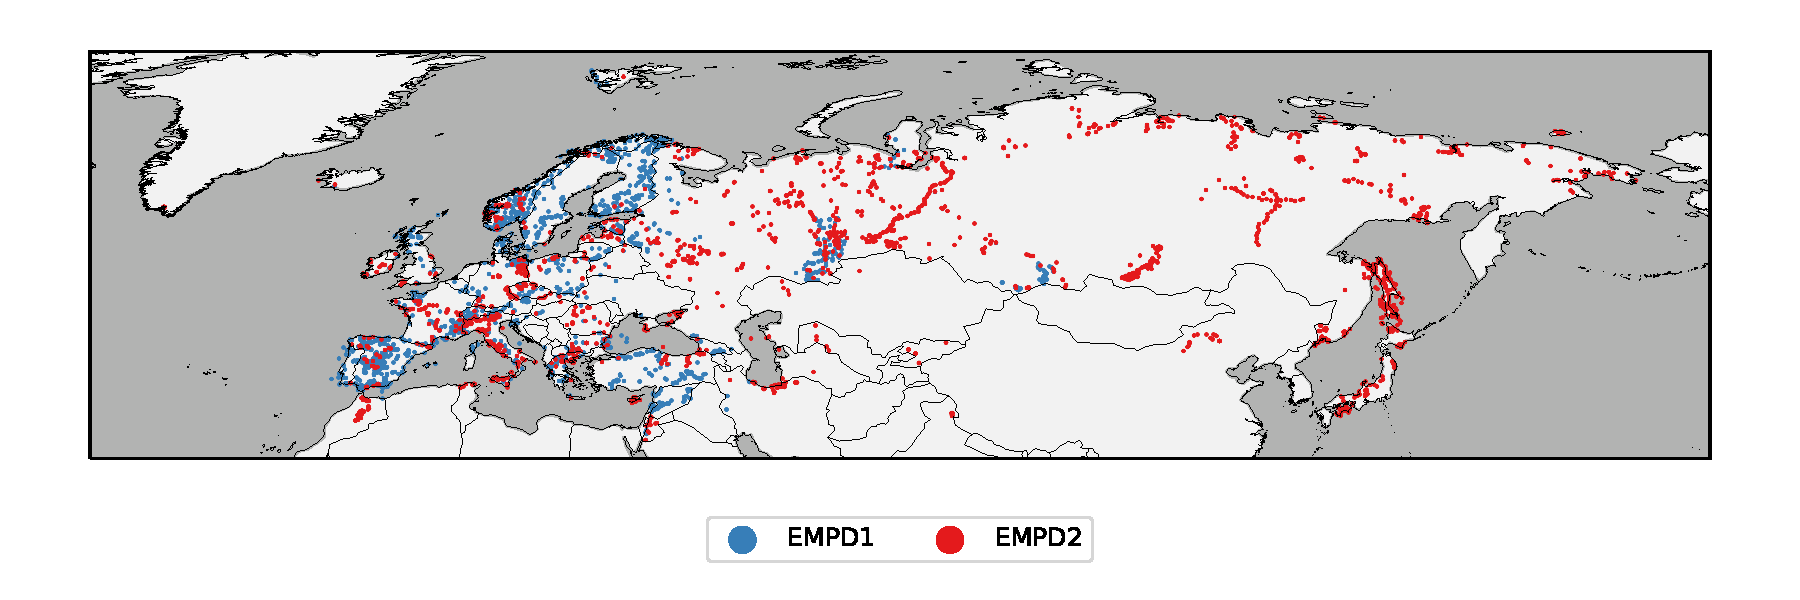
\includegraphics[width=\linewidth]{empd-figures/empd-sites.pdf}
	\caption[Modern calibration samples in the EMPD]{Modern calibration samples in the \gls{empd}.\todo[inline]{needs to be formatted (see printed version)}}
	\label{fig:empd-sites}
\end{figure}

The \glslink{empd}{Eurasian (née European) Modern Pollen Database (EMPD)} was established in 2013 as a public database of quality controlled and standardized modern pollen surface sample data to compliment the European Pollen Database (EPD) for fossil pollen \citep{DavisZanonCollinsEtAl2013}. The first version of the \gls{empd} (referenced herein as the \gls{empd}1) contained almost 5000 samples, submitted by over 40 individuals and research groups from all over Europe. Over the last 6 years more data has continued to be submitted, and more efforts have been made to incorporate more data held in open data repositories such as PANGAEA, and as supplementary information in published studies. This data is now released as the Eurasian Modern Pollen Database, version 2 \citep{DavisChevalierSommerEtAlinprep} with an increase of 80 percent to 8663 samples (see figure \ref{fig:empd-sites}).

The \gls{empd} remains the only public and open access database of modern pollen samples covering the Eurasian continent and is entirely driven by the community of its data contributors. This effort of creating an open and accessible database led to the development of new open source data management tools that we present in this chapter. The \gls{empd}2 is now hosted on the version control platform Github, with a dedicated web viewer at \href{https://EMPD2.github.io}{EMPD2.github.io} and an automated administration app, the \gls{empd}-admin (see table \ref{tab:empd-links} for a list of the web resources). The new web-viewer provides an intuitive interface into the database and displays the essential meta information for every sample, as well as the pollen and climate data in a comprehensive bar plot. The integration with the \gls{empd}-admin provides a simplified and transparent administration of multiple contributions from different sources and people to the database. All web components are hosted without any additional costs. The integration for the \gls{empd}, that we present here, is only one example of a regional database. This framework can be extended to make other community-based (regional) pollen databases accessible, for instance the \glsfirst{lapd} \citep{FlantuaHooghiemstraGrimmEtAl2015} or \glsfirst{apd} \citep{VincensLezineBuchetEtAl2007}. Especially the light-weight \gls{empd}-viewer web interface can be ported to other database (as shown in section \ref{sec:polnet-viewer}) to make heterogeneous data accessible to the broad public.

\begin{table}
	\caption{EMPD Web resources}
	\label{tab:empd-links}
	\begin{tabular}{|l|p{0.25\linewidth}|c|}
		\hline 
		& Description & Online Access \\ 
		\hline
		EMPD2 & Github Organization & \href{https://github.com/EMPD2}{github.com/EMPD2} \\
		\hline 
		\multirow{3}{*}{EMPD-Viewer} & \multirow{3}{\linewidth}{Map-based web interface to the EMPD database} & \href{https://github.com/EMPD2/EMPD-viewer}{github.com/EMPD2/EMPD-Viewer} \\
		& & \href{https://empd2.github.io/}{empd2.github.io} \\
		& & \\
		\hline 
		\multirow{3}{*}{EMPD-Data} & \multirow{3}{\linewidth}{Version controlled data repository of the EMPD} & \href{https://github.com/EMPD2/EMPD-data}{github.com/EMPD2/EMPD-data}  \\ 
		& & \\
		& & \\
		\hline 
		\multirow{3}{*}{EMPD-Admin} &  \multirow{3}{\linewidth}{Automated administration web app for the EMPD} & \href{https://github.com/EMPD2/EMPD-admin}{github.com/EMPD2/EMPD-admin} \\ 
		& & \href{https://empd-admin.herokuapp.com/}{empd-admin.herokuapp.com} \\ 
		& & \href{https://EMPD2.github.io/EMPD-admin}{EMPD2.github.io/EMPD-admin} \\ 
		\hline 
	\end{tabular} 
\end{table}

\section{The EMPD web framework}\label{sec:empd-web-framework}

The EMPD web framework is built on very common open source software development tools that have been adopted for a transparent data management, in favor of open science. The \gls{empd} is now hosted on the web platform Github at \href{https://github.com/EMPD2}{github.com/EMPD2}. This web platform, free of charge, hosts the source code for many popular open source software packages but can also be used to host a diverse, but small database (in terms of megabytes), such as the \gls{empd}. Github builts upon the version control system \textit{git} that transparently manages changes to documents by providing a full history of their revisions. The web platform is intrinsically designed for community-based projects that focus on collaboration and contains many features for a transparent communication between users, maintainers and contributors of a project. Besides others, the platform provides repository (i.e. project) specific discussion pages, so-called issues, where users can provide feedback, report bugs, or discuss any other aspect of the project. These issues are often linked to so-called pull requests, where each pull request is a proposal for a change in the source files of the project. This is then discussed between project maintainer and contributor in a dedicated discussion/review page.

Another common feature for Github repositories are integrations with so-called \glsfirst{ci} services, e.g. for automated testing and/or packaging the software. These services run predefined scripts (for example test scripts) every time someone contributes to the repository, or creates a pull request.

The following sections describe how these software development tools are implemented in the three components of the \gls{empd} web framework, the \gls{empd}-viewer (section \ref{sec:empd-viewer}), the \gls{empd} data repository (section \ref{sec:empd-data}) and the \gls{empd}-admin (section \ref{sec:empd-admin}).

\subsection{The EMPD viewer}\label{sec:empd-viewer}

\begin{figure}[h]
	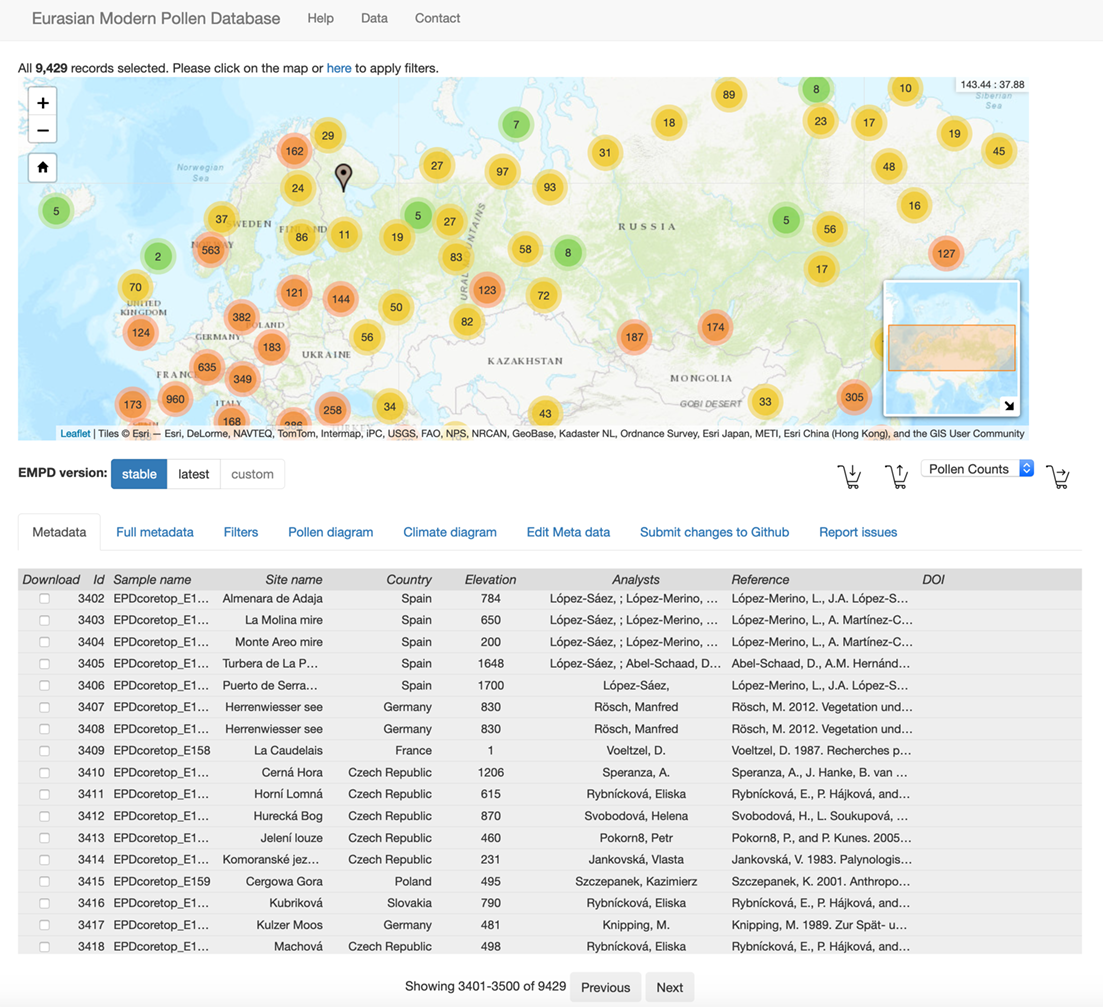
\includegraphics[width=\linewidth]{empd-figures/screenshot-compr.png}
	\caption{Screenshot of the EMPD viewer}
	\label{fig:empd-viewer}
\end{figure}

The main public interface into the \gls{empd} is an interactive web viewer accessible
from \href{https://EMPD2.github.io}{EMPD2.github.io}. This JavaScript-based application (see figure \ref{fig:empd-viewer} for a screenshot) provides an intuitive interface into the database without requiring any particular computer expertise. It enables the user to view the data on a map and to select and download subsets of the database. The webpage involves no server-side processing and such it can be hosted for free using the service provided by Github Pages (\href{https://pages.github.com/}{pages.github.com}). This provides a stable access to the database, independent of funding availabilities.

\subsubsection{The Web Interface}

The EMPD-Viewer has been initially based on the climate proxies finder \citep{BollietBrockmannMassonDelmotteEtAl2016, Brockmann2016} which can still be seen in it the layout and design of its graphical interface (i.e. its front-end). The code base, however, has been changed entirely, updated to the latest available versions of the underlying JavaScript dependencies and extended with multiple additional tools, shown in table \ref{tab:empd-viewer-tools}. The central element of the viewer is a map to show the sample locations. It also allows to intuitive access to the essential meta data of every sample through the popup of the corresponding marker on the map. The detailed meta data can also be seen in the meta data table, together with all the other samples. Another key element of the viewer are the meta data filters, that subset the data using efficient and intuitive filtering tools. This allows to search the database\todo{needs implementation}, or to select specific countries, climatic regimes, sample types, samples of a specific data contributor/analyst, and more.

Additional information on the sample is revealed through a bar diagram of the associated pollen data, which is dynamically created when the user clicks on the sample. The viewer also displays monthly, seasonal and annual precipitation and temperature values at the side, based on the WorldClim dataset, version 2 \citep{FickHijmans2017}.

Finally, the viewer contains elements that allow scientists to contribute to the database, even without dedicated knowledge about the Github framework. The meta data editor allows to edit a sample and then submit it via the data submission form. The request is handled by the \gls{empd}-admin webapp (see section \ref{sec:empd-admin}) that pushes the data to the corresponding pull request on Github that is then reviewed by the core database maintainers. Another implemented element is an issue report form that allows the user to highlight erroneous sample information which is then, again through the \gls{empd}-admin, submitted as a Github issue to the data repository.

The web app is fully integrated into the Github framework of the \gls{empd} and loads the displayed data from the online repository. As such, it also provides a further quality control check and allows the data contributors/maintainers to review and edit new contributions before they are merged into the database.

\afterpage{
	\begin{longtable}{c}
		\caption[Tools in the EMPD viewer]{Tools in the \gls{empd} viewer} \label{tab:empd-viewer-tools} \\
		\endfirsthead
		\caption{Tools in the EMPD viewer (continued)}
		\endhead
		\hline
		\tabularnewline
		Map interface \\
		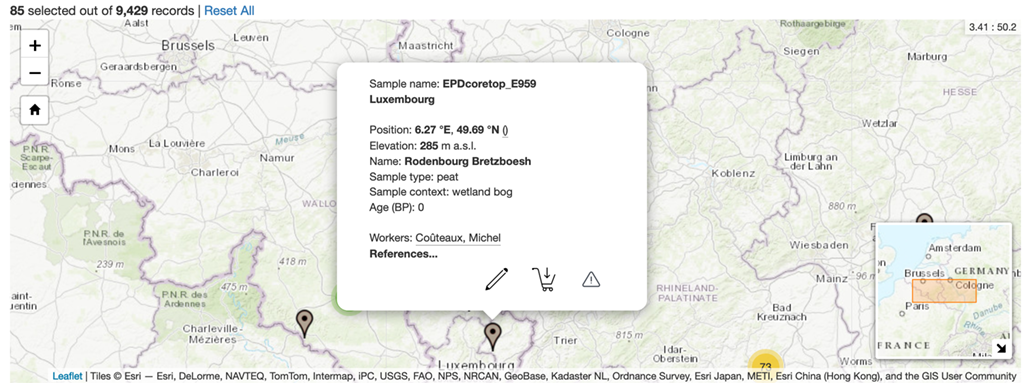
\includegraphics[width=\linewidth]{empd-figures/map-compr.png} \\
		\todo[inline]{may need a higher resolution} \\
		\hline\hline
		\tabularnewline
		Meta data table \\
		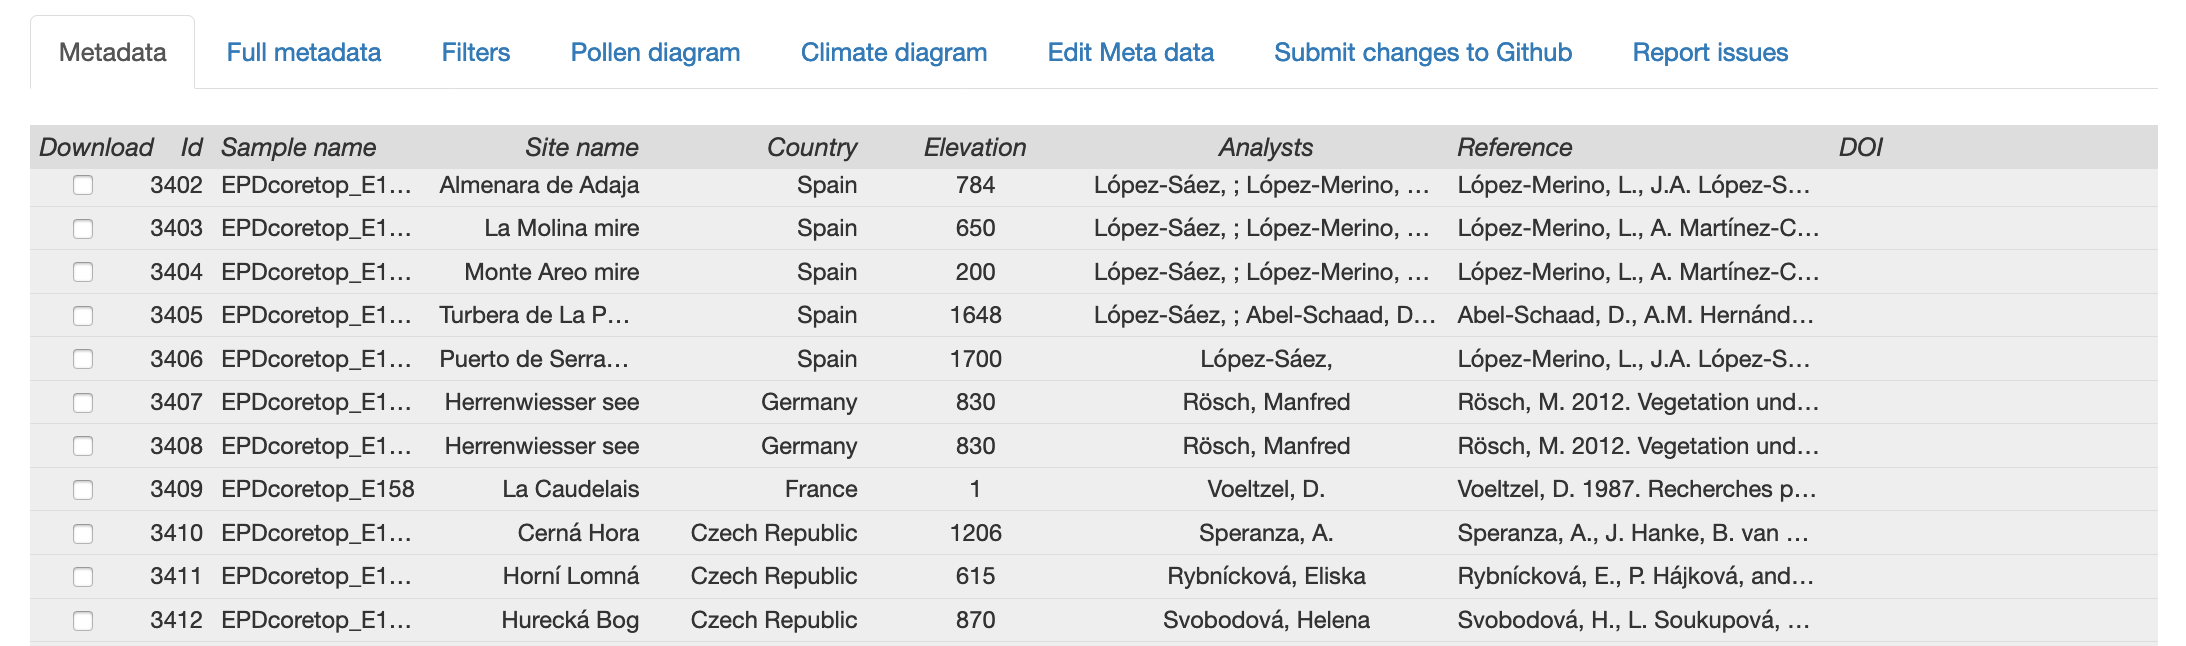
\includegraphics[width=\linewidth]{empd-figures/meta-data-table.png} \\
		\hline\hline
		\tabularnewline
		Pollen Data \\
		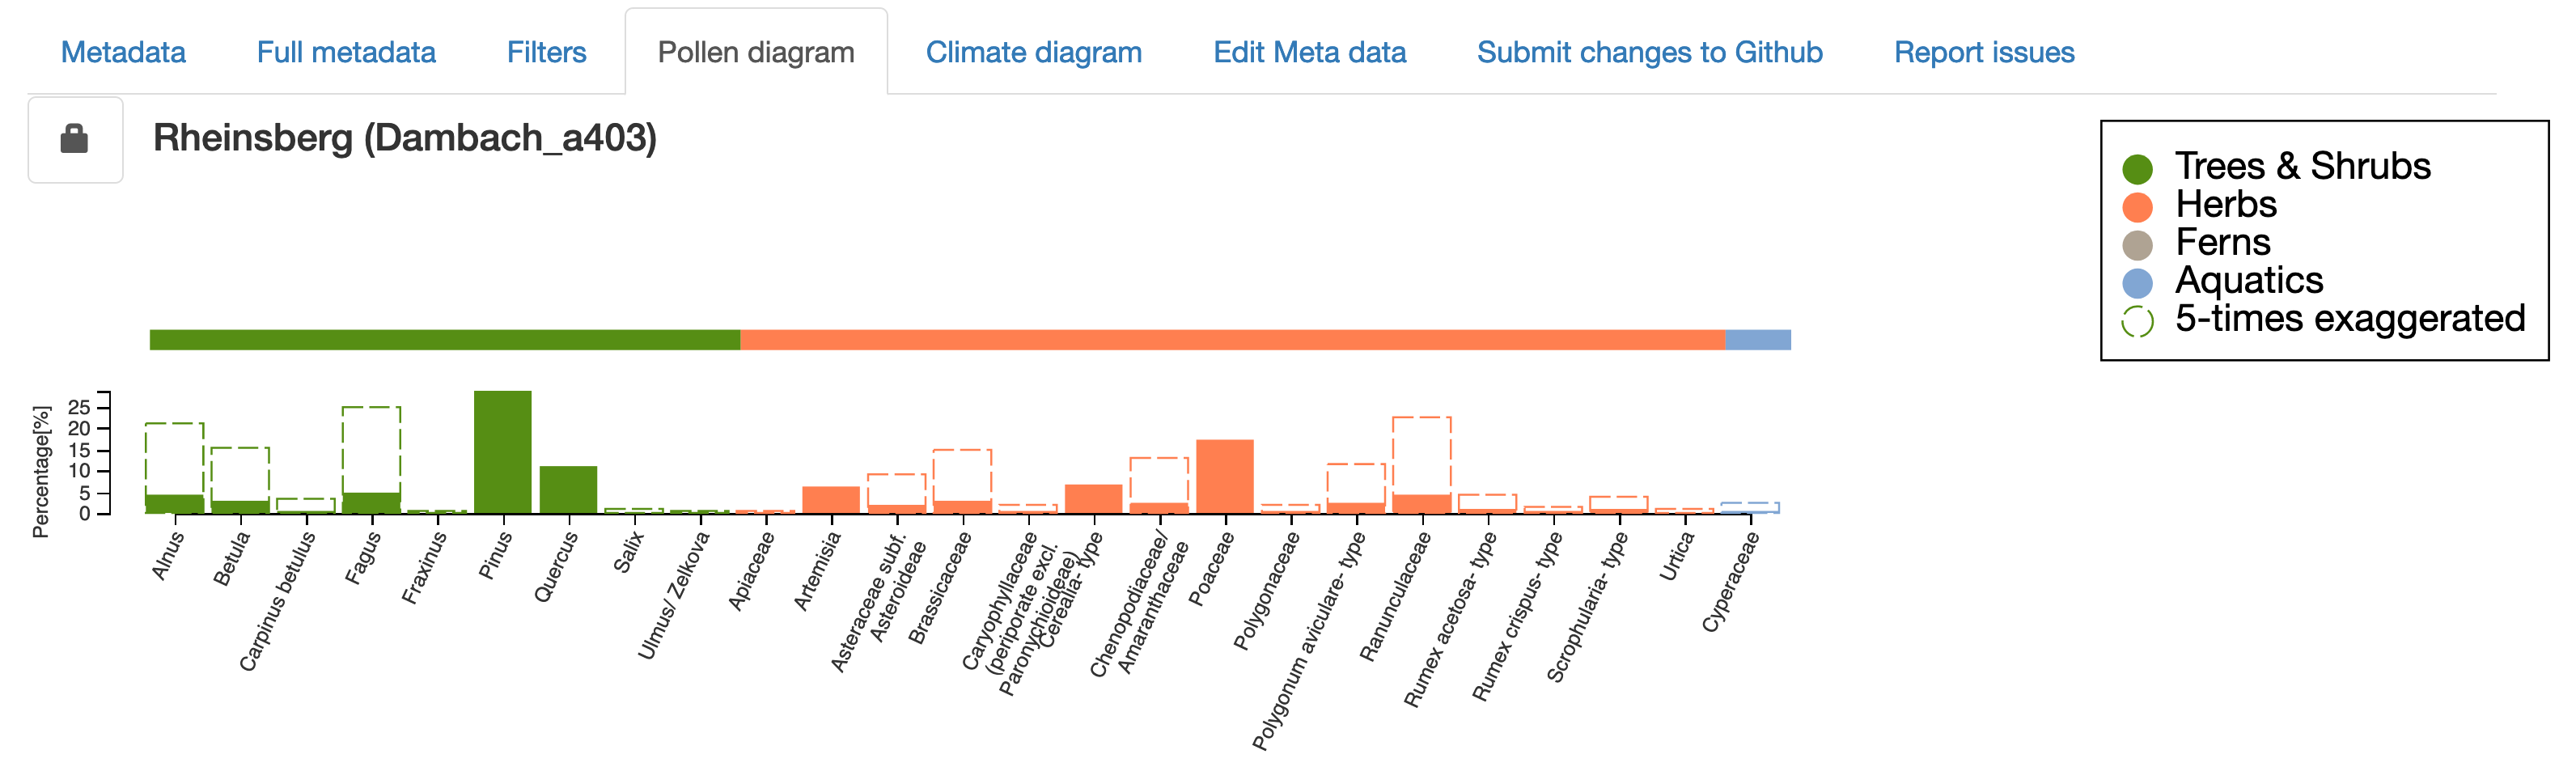
\includegraphics[width=\linewidth]{empd-figures/pollen-bar-diagram.png} \\
		\hline\hline
		\tabularnewline
		Climate Data \\
		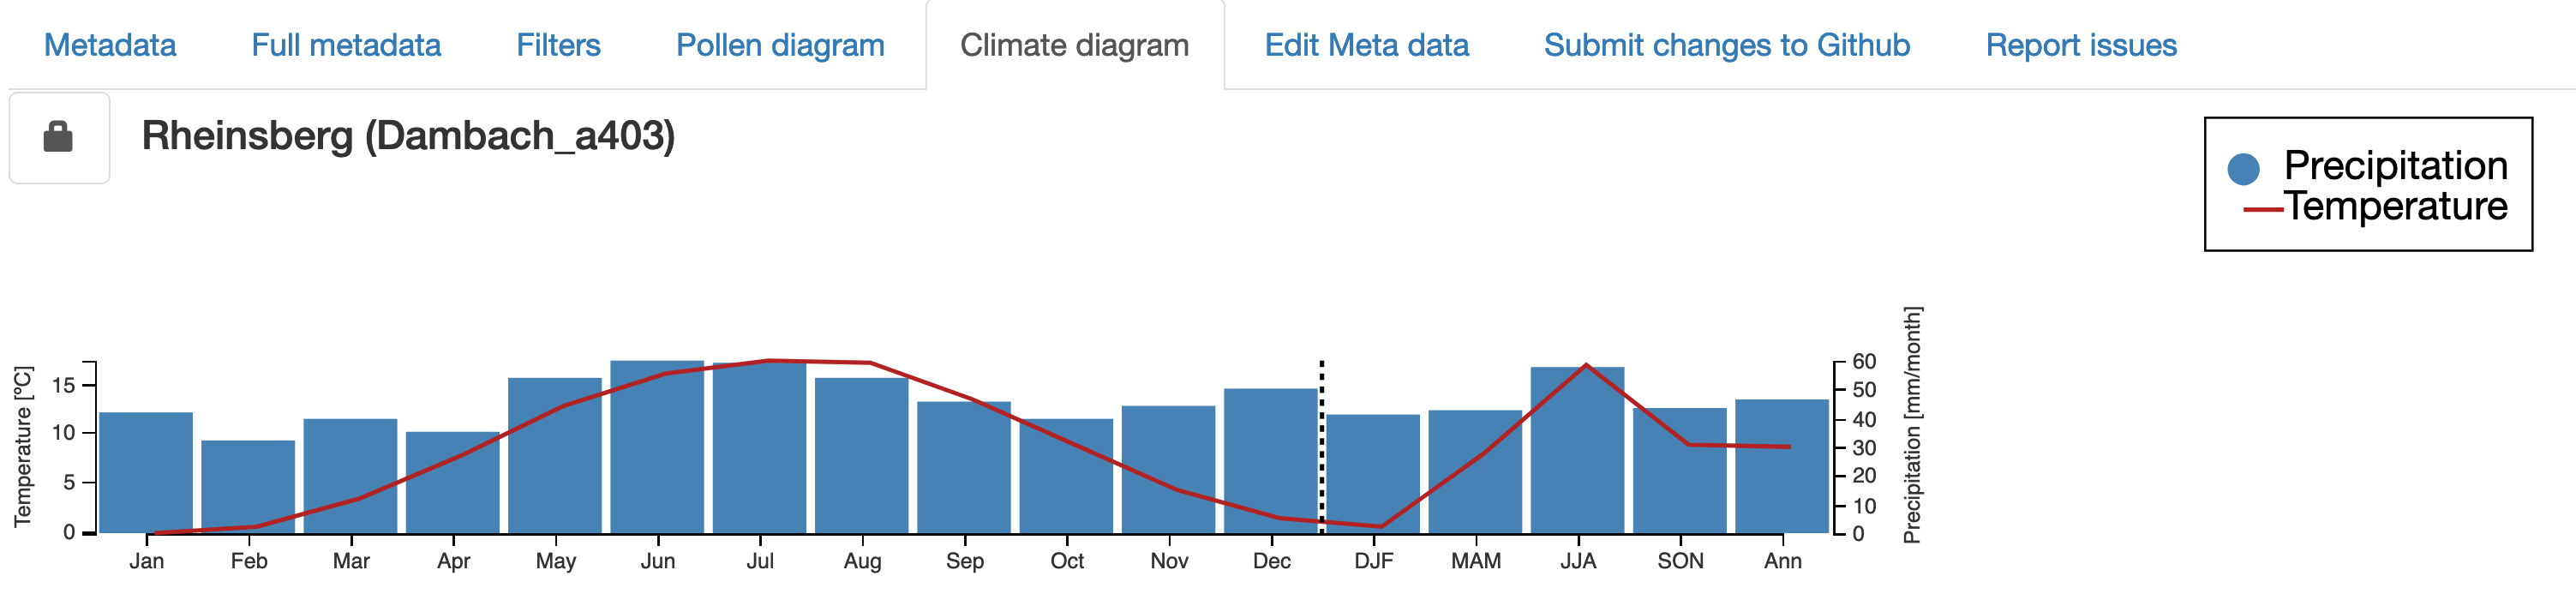
\includegraphics[width=\linewidth]{empd-figures/climate-diagram.png} \\
		\newpage \\
		\hline
		\tabularnewline
		Meta data filter \\
		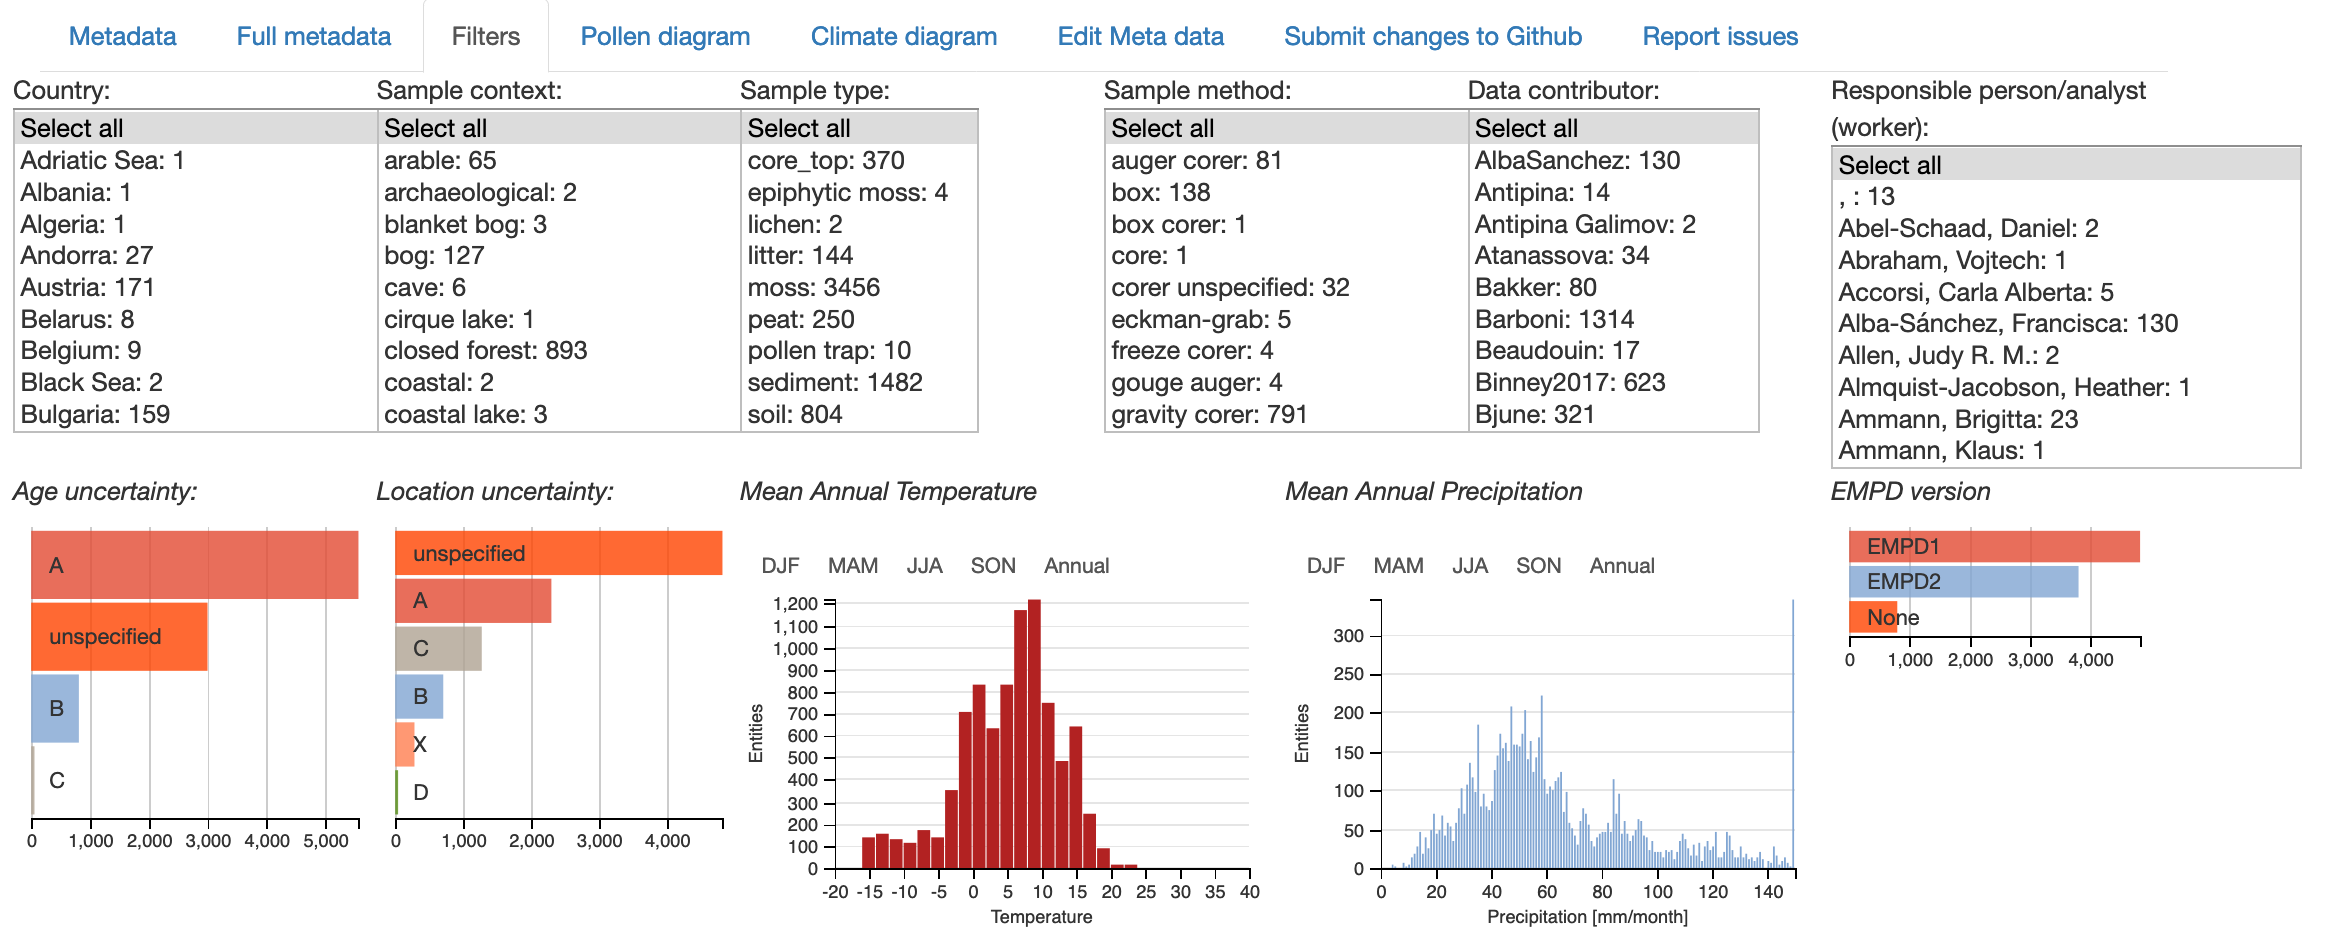
\includegraphics[width=\linewidth]{empd-figures/filter.png} \\
		\hline
		\tabularnewline
		Meta Data Editor \\
		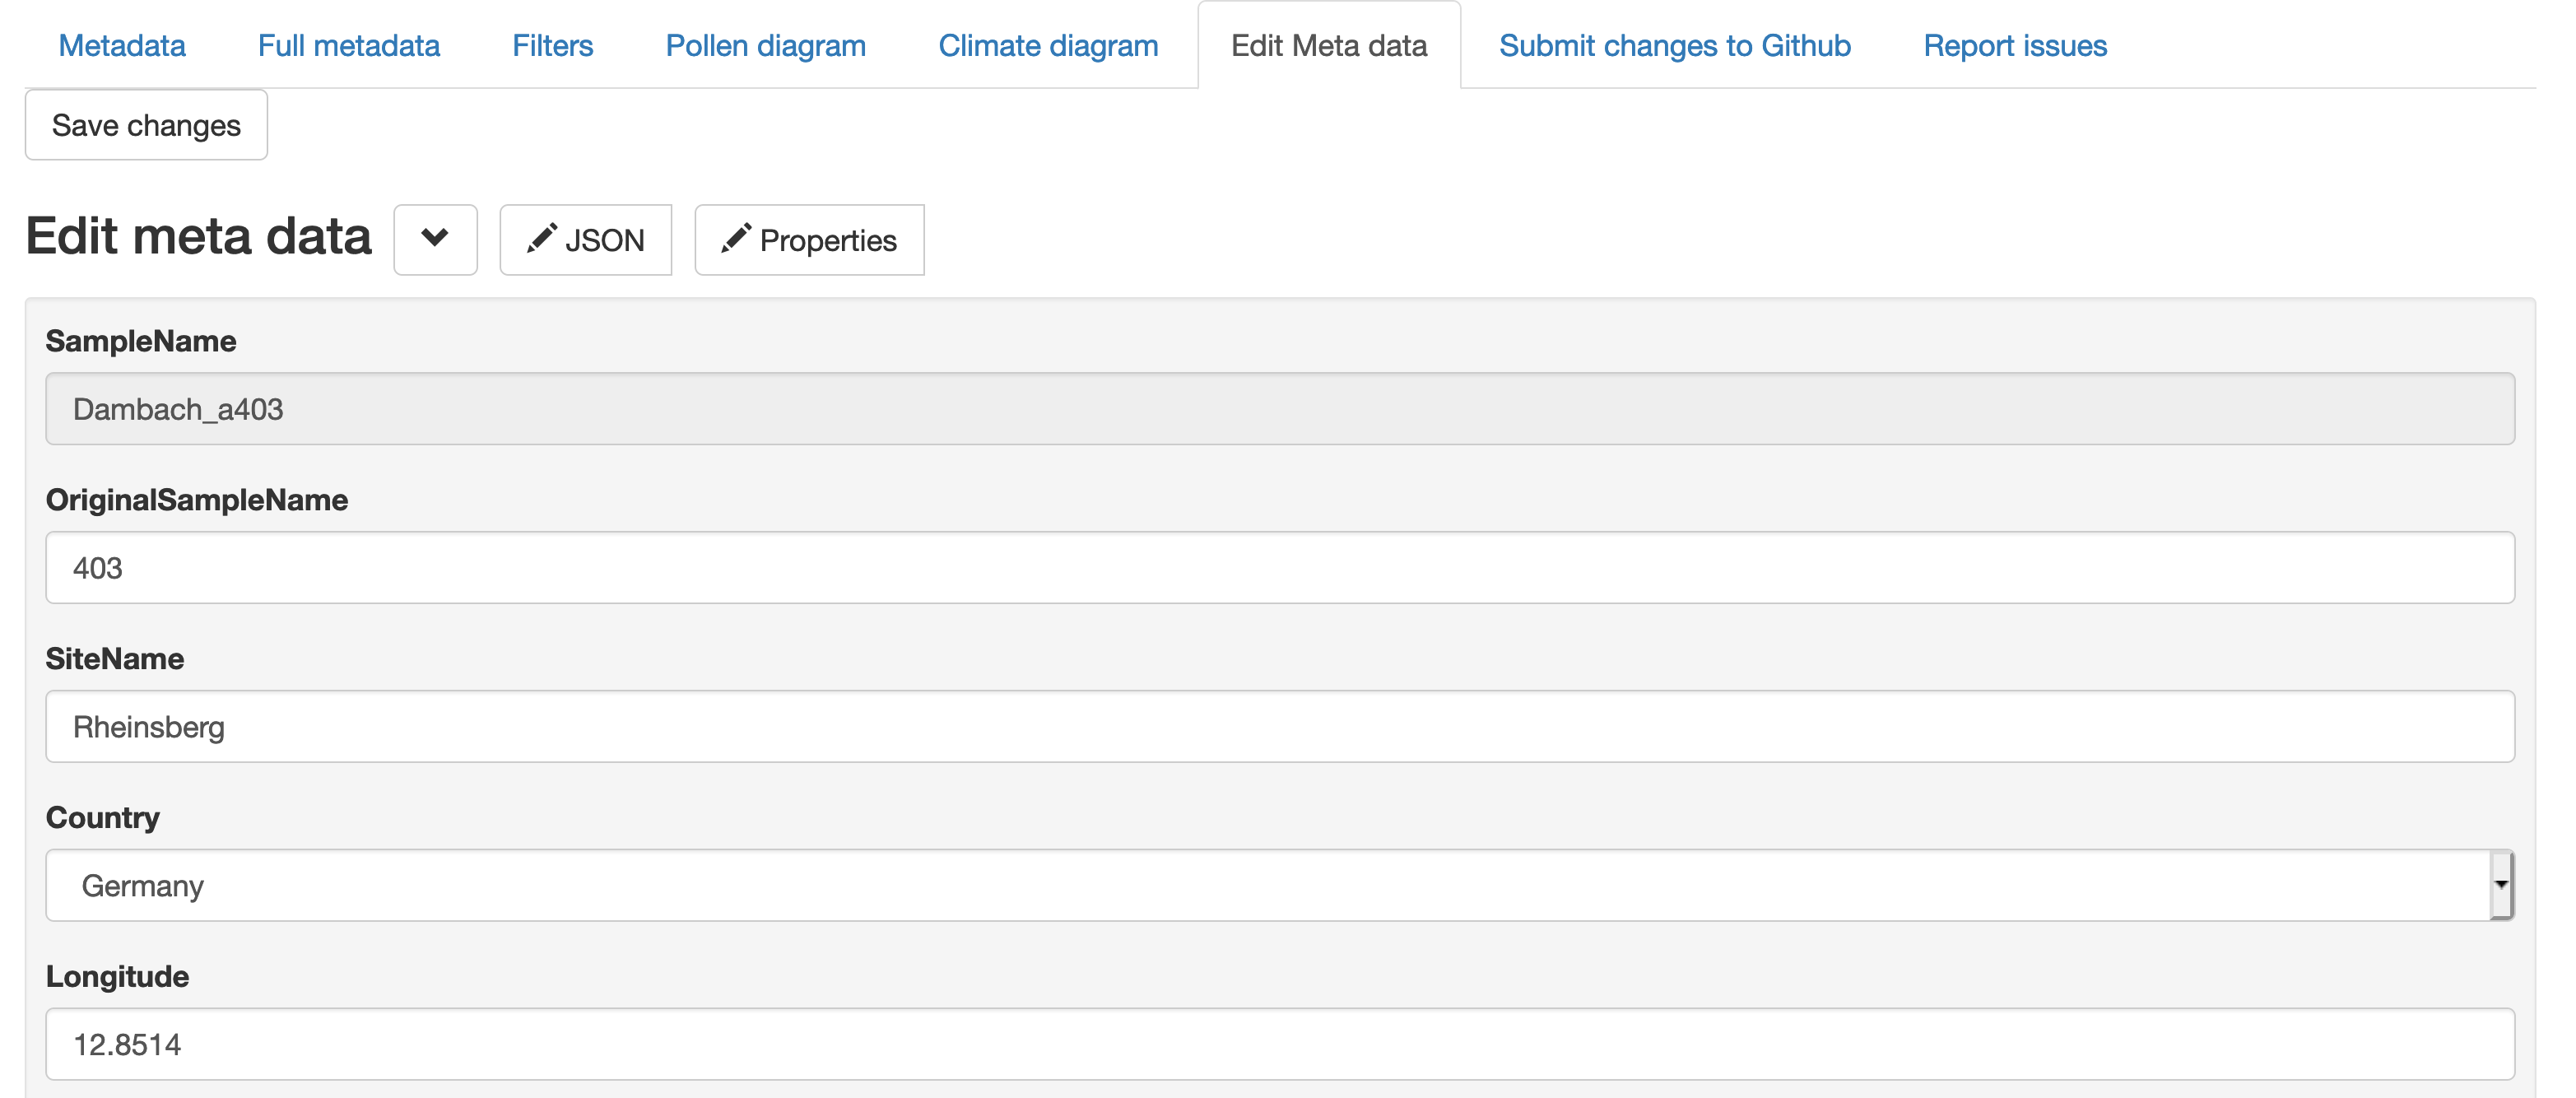
\includegraphics[width=\linewidth]{empd-figures/meta-data-editor.png} \\
		\hline
		\tabularnewline
		Issue submission form \\
		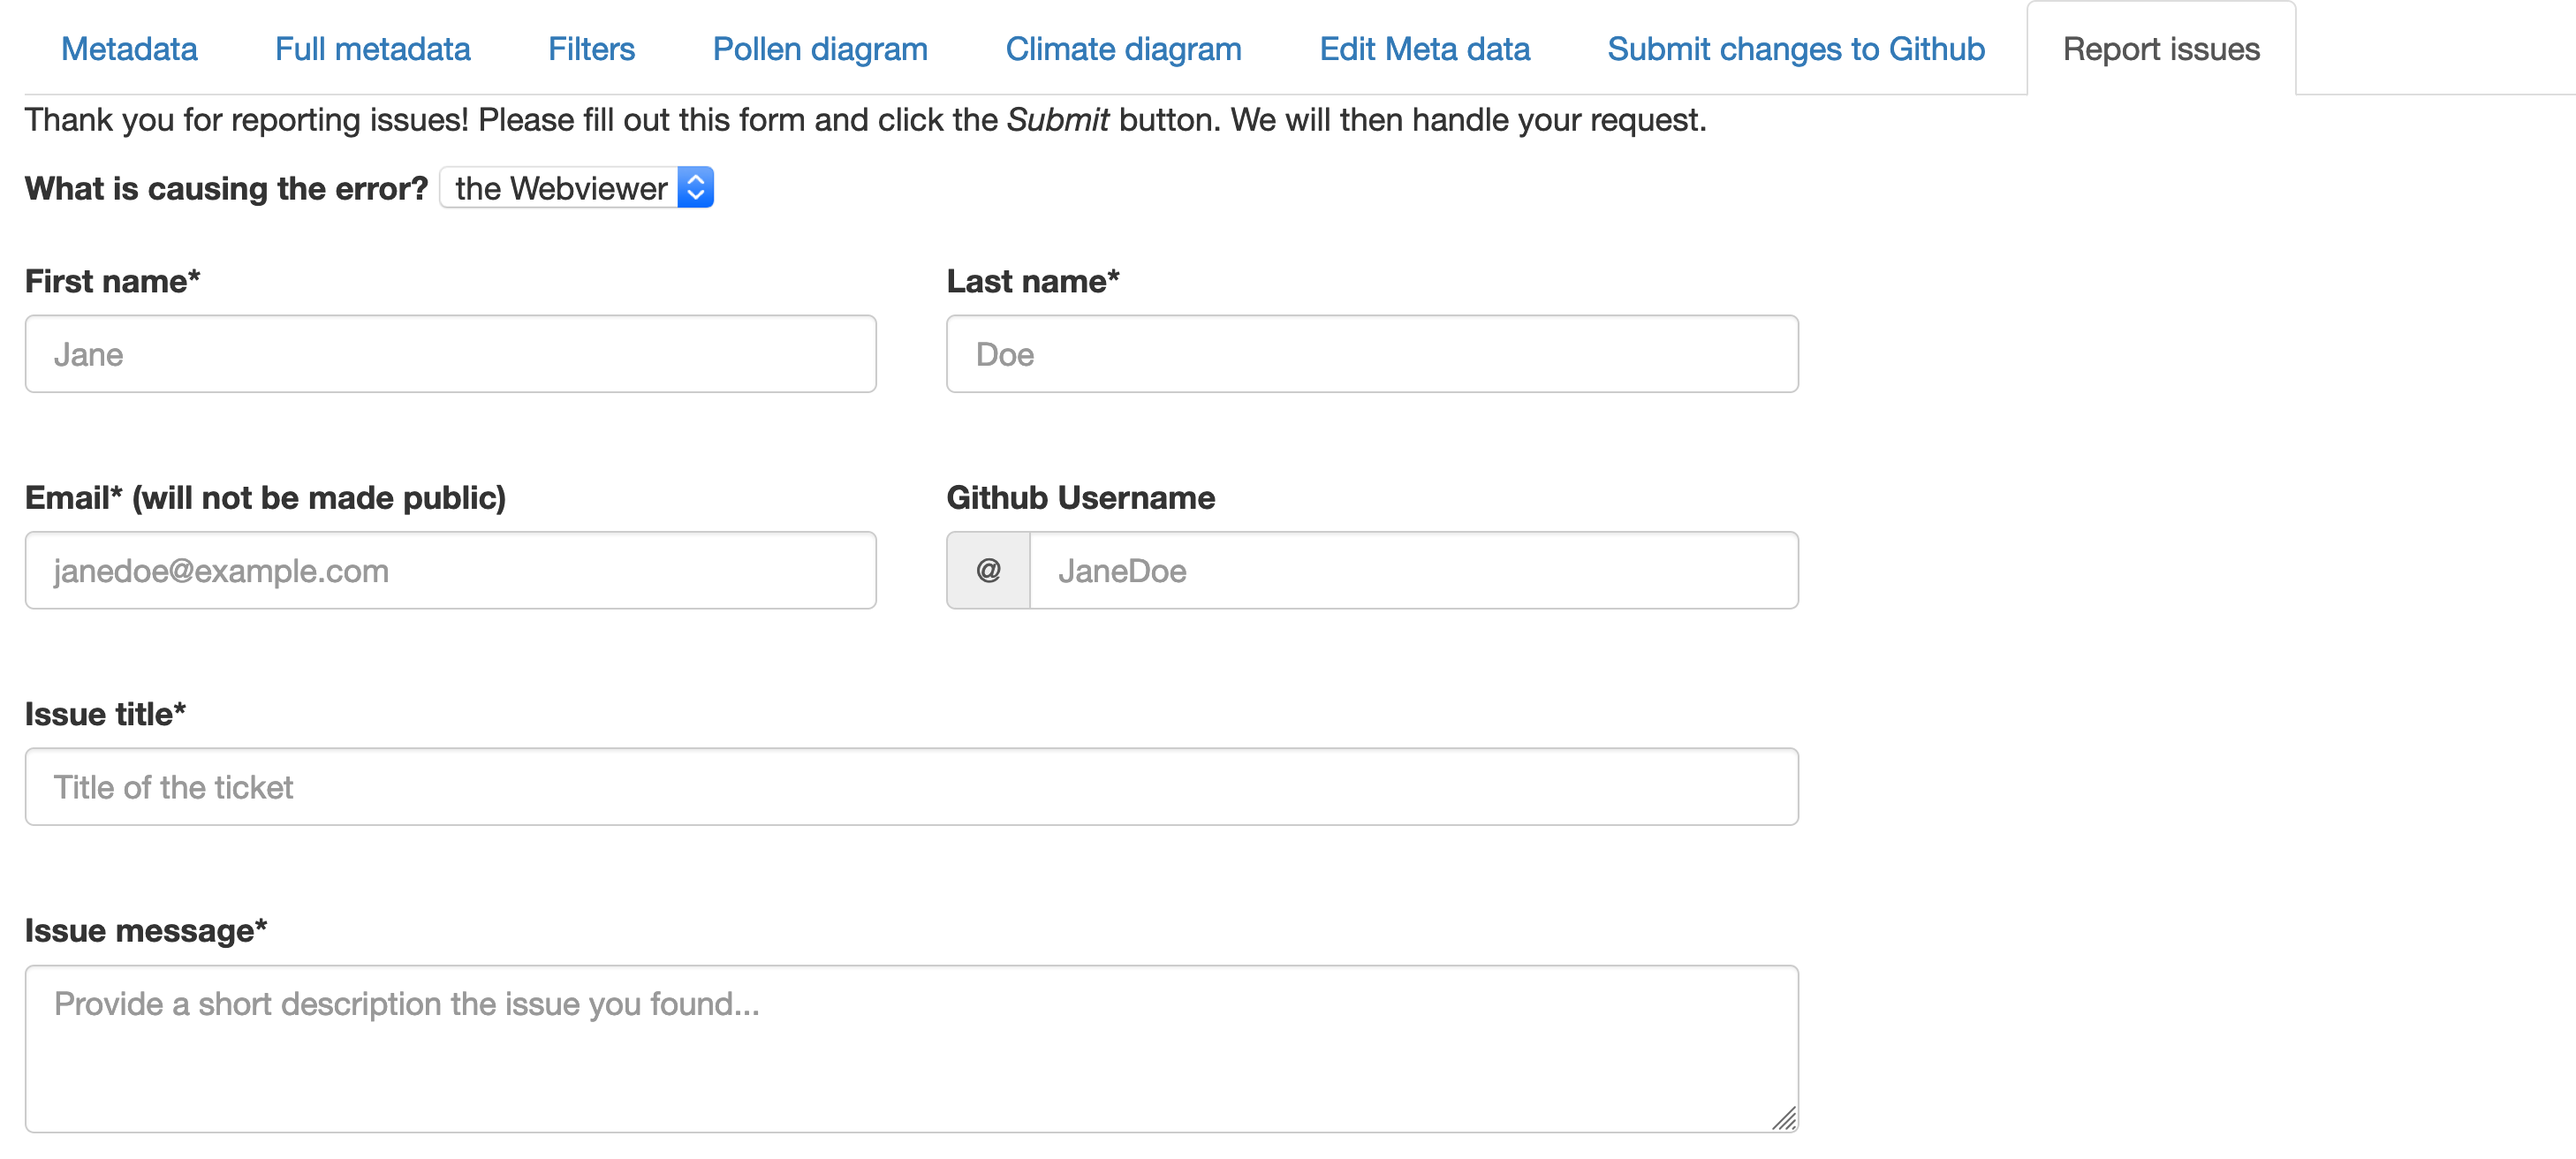
\includegraphics[width=\linewidth]{empd-figures/issue-report.png} \\
		\hline\hline
	\end{longtable}
}

\subsubsection{Implementation details}

The viewer itself is very light-weight and can be flexibly adapted to other database systems (see for example section \ref{sec:polnet-viewer}). As the climate proxies finder \citep{BollietBrockmannMassonDelmotteEtAl2016, Brockmann2016}, the \gls{empd}-viewers main viewing/filtering functionality it is built upon the \textit{dc} \citep{ZhuDevelopers2019}, \textit{crossfilter} \citep{Squarecrossfiltercontributors2019} and \textit{leaflet} \citep{Agafonkin2019} open source JavaScript libraries. We ported the app to the \textit{npm} package manager (\href{https://www.npmjs.com/}{npmjs.com}) which enables a better and more secure monitoring of the app dependencies. This package manager is also used for an automated testing of the viewer on a \gls{ci} service, prior to deployment on the official web page. Due to time constrains, the viewer is not yet fully adapted to mobile devices. 

\subsection{The EMPD2 data repository}\label{sec:empd-data}

The raw data of the EMPD2 is accessible as plain text files in the \textit{EMPD-data} Github repository (see table \ref{tab:empd-links}). The software development framework of Github (see introductory part of section \ref{sec:empd-web-framework}) is adopted such that issues in the data repository can highlight errors in the database, or provide room for the discussion of potential new efforts that should be considered within the community-database. Pull requests into the repository are new data contributions that can be reviewed by the maintainers before being merged into the official database.

This \DIFdelbegin \DIFdel{methodology }\DIFdelend \DIFaddbegin \DIFadd{method }\DIFaddend allows a fully transparent traceback of changes made to the EMPD through version control. The online access to the raw data files through Github also allows the EMPD viewer to interface with different versions of the database (see previous section). 

The EMPD-data repository additionally uses the \gls{ci} services from Travis CI (\href{https://travis-ci.org/}{travis-ci.org}) for automated tests of the meta data in each sample. 


\subsection{The EMPD-admin}\label{sec:empd-admin}

In addition to the standard \gls{ci} services, we developed the \gls{empd}-admin webapp. Inspired by the web management tools of the conda-forge community\DIFdelbegin \DIFdel{(}%DIFDELCMD < \href{https://conda-forge.org}{conda-forge.org}%%%
\DIFdel{)}\DIFdelend \DIFaddbegin \footnote{\href{https://conda-forge.org}{conda-forge.org}}\DIFaddend , this tool provides an automated handling of data contributions from within Github Pull Requests. It behaves like a standard \gls{ci} service and runs tests on the data contribution, every time changes have been made to the pull request. 

But the main purpose of the EMPD-admin is to provide a web tool for an automated administration of the database, which is helpful for a community-project with changing maintainers. Hence, the \gls{empd}-admin web app acts like a bot that reacts on comments from within a pull request (i.e. a data contribution). Maintainers and contributors can use this functionality and directly contact the bot, for instance, to subset the data, run specific tests on subsets of the data, or automatically fix certain meta data issues, such as wrong countries or missing elevation. 

The bot is also integrated in the \gls{empd}-viewer (see previous section \ref{sec:empd-viewer}). Bug reports or edited data are processed by the \gls{empd}-admin and put online as an issue in the github repository, or it updates the corresponding data contribution.

As such, the administration of the database can be done entirely remotely, without having to install dedicated software on a local computer.

\subsubsection{Implementation details}
The EMPD-admin webapp is hosted for free at Heroku (https://www.heroku.com) at \href{https://empd-admin.herokuapp.com/}{empd-admin.herokuapp.com} with a software package documentation hosted at \href{https://EMPD2.github.io/EMPD-admin}{{EMPD2.github.io/EMPD-admin}}. This, again, allows stability independent on the availability of funding. The package can, also be installed locally and used from the command-line, independent of Github and Heroku, which is sometimes helpful for very large data contributions..

The Python library is based on the tornado web framework\DIFdelbegin %DIFDELCMD < \href{https://www.tornadoweb.org/en/stable/}{www.tornadoweb.org}%%%
\DIFdelend \DIFaddbegin \footnote{\href{https://www.tornadoweb.org/en/stable/}{www.tornadoweb.org}}\DIFaddend , as well as pandas \citep{McKinney2010}, a tabular data analysis library for Python, and sqlalchemy \citep{Bayer2012}, a Python SQL toolkit.

\subsection{Distribution of the tools}\label{sec:empd-accessibility}

The \gls{empd} is hosted within the \gls{empd}2 Github organization (\href{https://github.com/EMPD2}{github.com/EMPD2}) \DIFdelbegin \DIFdel{at }%DIFDELCMD < \href{https://github.com/EMPD2/EMPD-data}{{github.com/EMPD2/EMPD-data}}%%%
\DIFdelend \DIFaddbegin \DIFadd{in the }\href{https://github.com/EMPD2/EMPD-data}{{EMPD-data}} \DIFadd{repository}\DIFaddend . The source files of the viewer are accessible \DIFdelbegin \DIFdel{at
}%DIFDELCMD < \href{https://github.com/EMPD2/EMPD-viewer}{{github.com/EMPD2/EMPD-viewer}}%%%
\DIFdelend \DIFaddbegin \DIFadd{in the
}\href{https://github.com/EMPD2/EMPD-viewer}{{EMPD-viewer}}\DIFaddend , and for the \gls{empd}-admin in the {\DIFdelbegin %DIFDELCMD < \href{https://github.com/EMPD2/EMPD-admin}{{EMPD2/EMPD-admin}}%%%
\DIFdelend \DIFaddbegin \href{https://github.com/EMPD2/EMPD-admin}{{EMPD-admin}}\DIFaddend } repository (see also table \ref{tab:empd-links}).

The \gls{empd}-data and the \gls{empd}-admin are additionally both available as so-called Docker container image at \url{https://hub.docker.com/u/empd2}. These containers are lightweight, standalone, executable packages of software that include everything needed to run an application: code, runtime, system tools, system libraries and settings. As such, they extend standard software packaging systems by providing an entire operating system that contains the target application. This makes it especially useful for web applications (such as the \gls{empd}-admin) that can, as such, operate in a well-defined and portable environment.

The EMPD-admin can, however, also be installed through the standard python package manager \texttt{pip}.

\section{The POLNET viewer} \label{sec:polnet-viewer}

\begin{figure}
	\centering
	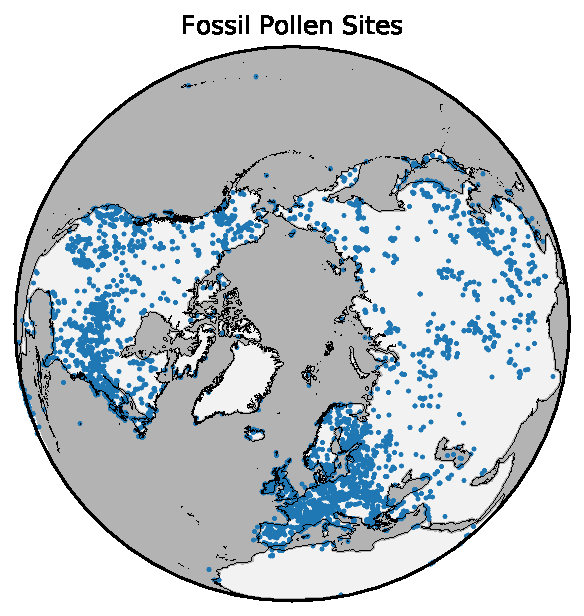
\includegraphics[width=0.45\linewidth]{empd-figures/fossil-sites.pdf}
	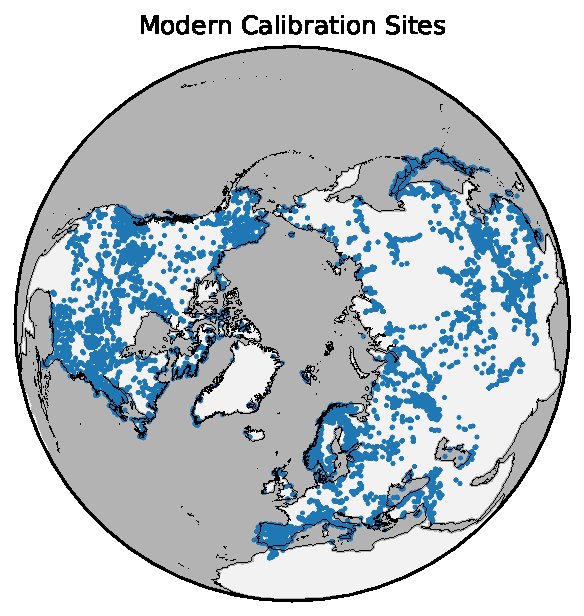
\includegraphics[width=0.45\linewidth]{empd-figures/modern-sites.pdf}
	\caption[Map of sites in the POLNET database]{Maps of (left) fossil and (right) modern pollen sites in the POLNET database.\todo[inline]{obscure grey part in printed version}}
	\label{fig:polnet-sites}
\end{figure}

\begin{figure}[h]
	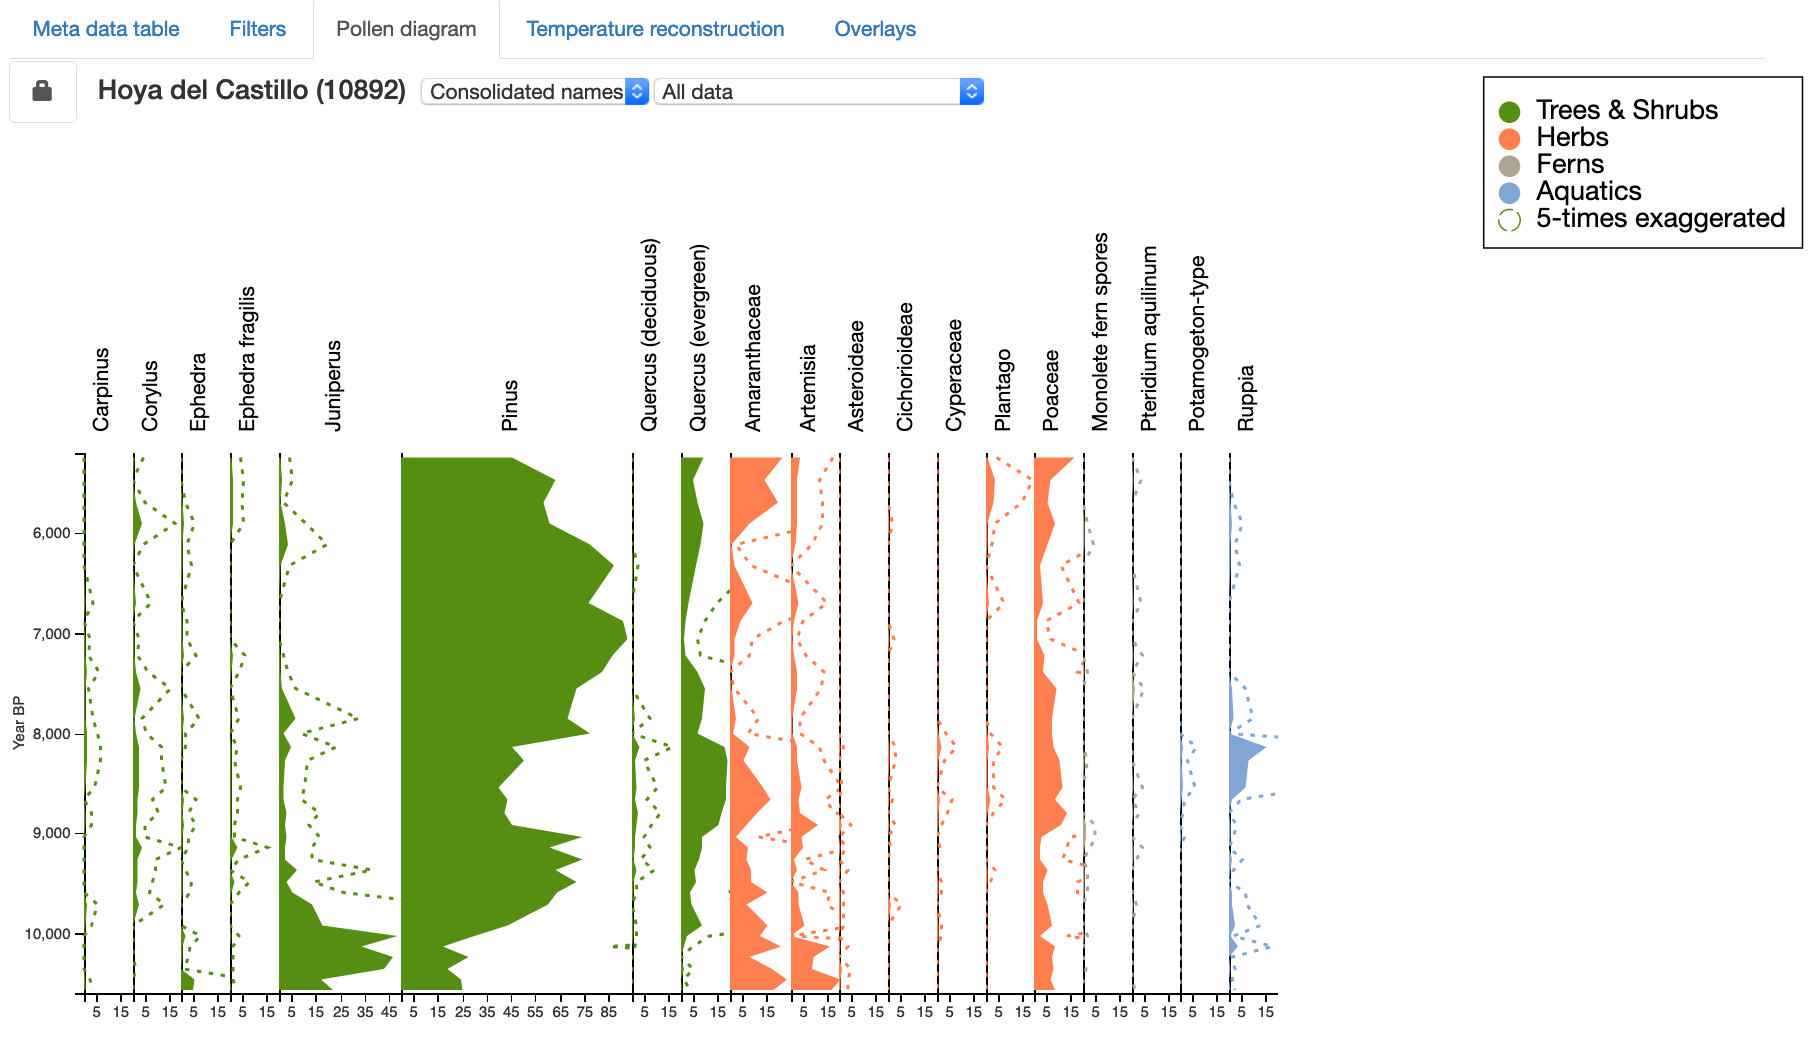
\includegraphics[width=\linewidth]{empd-figures/polnet-diagram.png}
	\caption{Screenshot of an automatically generated pollen diagram in the POLNET database viewer. The left dropdown menu above the pollen diagram allows to select the different naming schemes (here consolidated names that were used for the pollen-climate reconstruction). The right dropdown menu selects either the entire data or specific samples that are then displayed as a bar diagram (see the pollen data in table \ref{tab:empd-viewer-tools}).}
	\label{fig:polnet-pollen-diagram}
\end{figure}

\begin{figure}[h]
	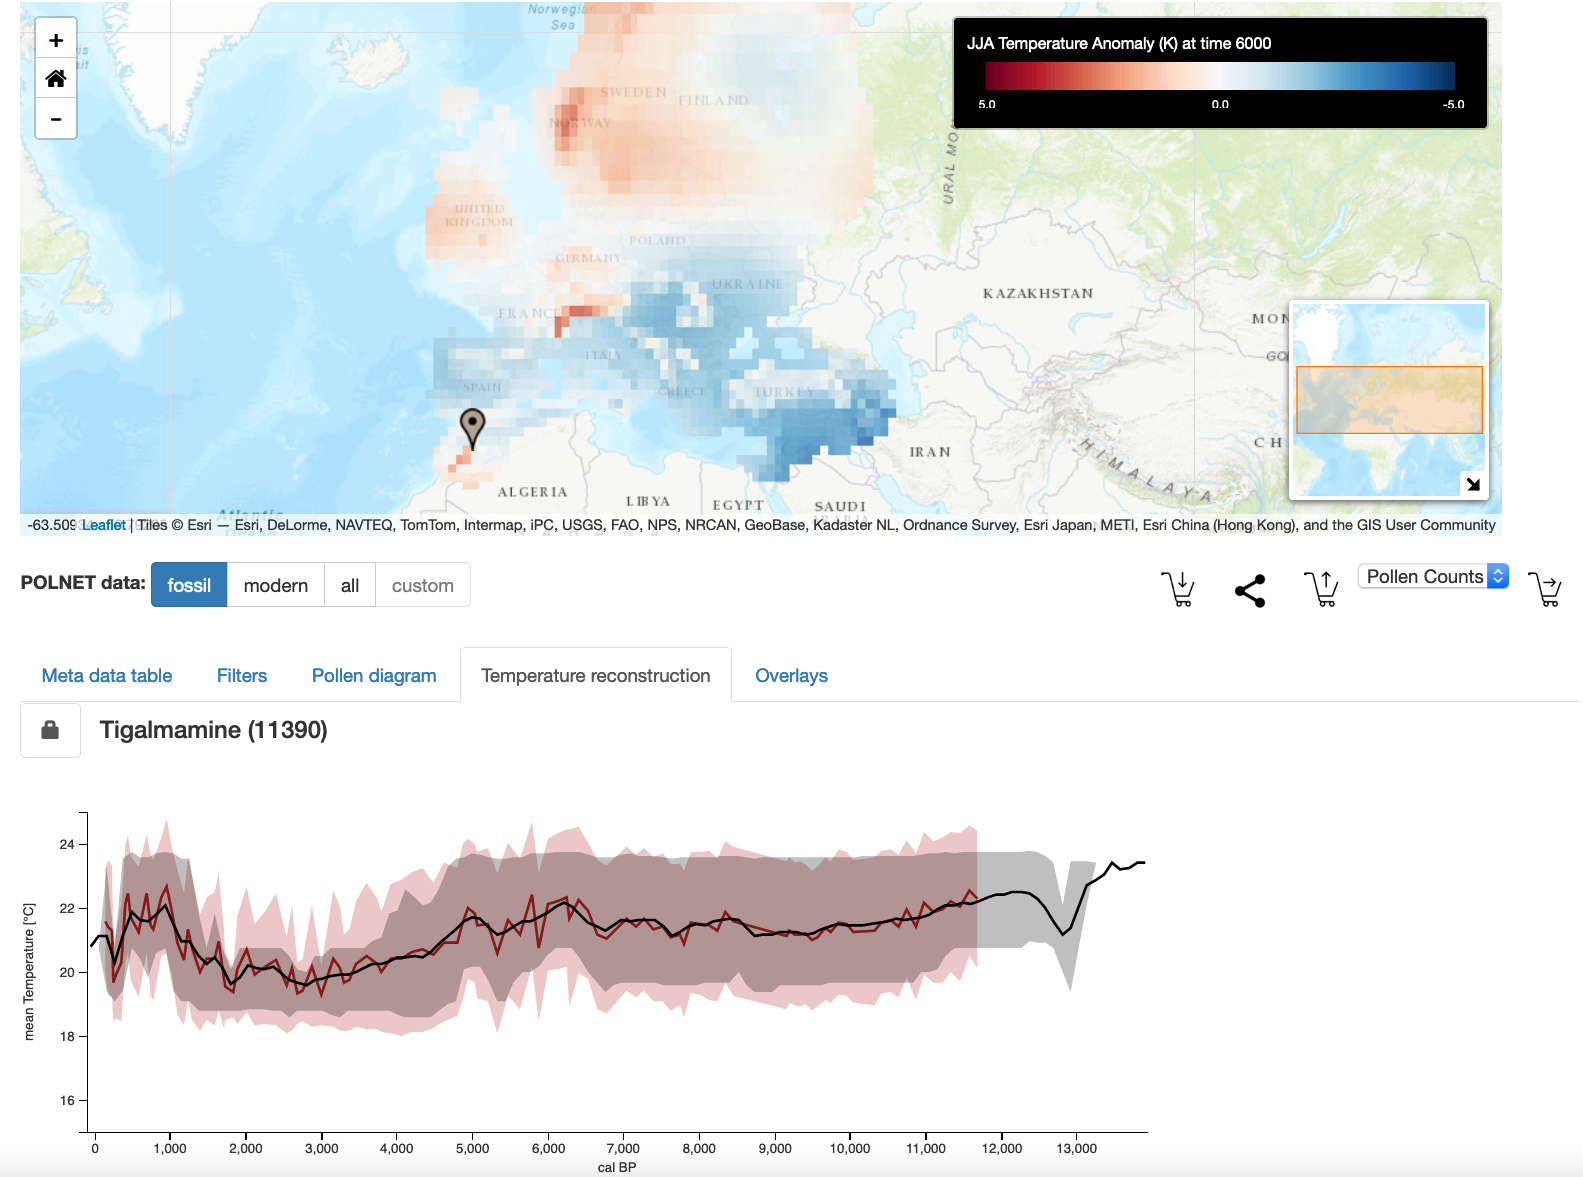
\includegraphics[width=\linewidth]{empd-figures/polnet-climate-plots.png}
	\caption[Climate reconstructions visualized in the POLNET viewer]{Exemplary screenshot how the climate reconstruction is visualized in the POLNET viewer. The map at the top figure shows the gridded temperature reconstruction (here 6k BP after \cite{MauriDavisCollinsEtAl2015}). The lower plot shows the single site-based reconstruction (here Tigalmamine \citep{CheddadiLambGuiotEtAl1998}) for different reconstruction methods.}
	\label{fig:polnet-climate}
\end{figure}

The adaptability of the \gls{empd}-viewer gave the motivation for an application with the POLNET database. This database, currently in development status, is a northern hemispheric, extra-tropical collection of modern and fossil pollen assemblages \citep{DavisKaplan2017, SommerDavisChevalierEtAl2019}. The purpose of this database is to generate the source for large-scale climate reconstruction during the Holocene (past 12'000 years) that can be used for model-data comparisons. It contains about 3'300 fossil pollen sites and about 13'200 modern surface samples (see figure \ref{fig:polnet-sites}) and is at present the largest existing collection of fossil and modern pollen samples. The database will soon be made publicly available through a dedicated web interface, the POLNET viewer. We present it here as a sample application of the EMPD-viewer to demonstrate how this web interface can be extended and applied to other datasets, in order to make them more accessible.

Like its core application, the \gls{empd}-viewer, the POLNET-viewer is a map-based interface with implemented meta data filters. As it is a data exploration and distribution tool only, we did not include the functionalities to edit the meta data or to submit issues. Instead we implemented new features to visualize the essential aspects of this database: fossil pollen data and climate reconstructions.

The fossil pollen data is loaded upon request from the dedicated Github repository. It is afterwards visualized in form of a stratigraphic pollen diagram, with the age of the samples on the vertical y-axis, and the pollen taxa organized as vertically aligned diagram columns (see figure \ref{fig:polnet-pollen-diagram}).

Climate reconstructions are displayed in two different manners: The site-based reconstructions are visualized as line plots in a separate diagram, together with their associated uncertainties. The gridded temperature reconstruction, i.e. the final product of the database (see also chapter \ref{chp:gridding}) is visualized as an overlay on the map of the web application. This results in a combined visualizations of site-based and gridded reconstructions (see figure \ref{fig:polnet-climate}) which enables an intuitive regional analysis of the reconstruction method.

\clearpage

\printbibliography[heading=subbibintoc]

\end{refsection}
% straditize chapter

\Chapter{Straditize}{A digitization software for pollen diagrams}

\label{chp:straditize}

\newcommand{\samplediagram}[1][false]{
	\ref{fig:sample-diagram}\hyperref[fig:sample-diagram]{
		\ifthenelse{\equal{#1}{false}}{}{#1)}}}

%----------------------------------------------------------------------------------------
%	SECTION 1
%----------------------------------------------------------------------------------------

\begin{refsection}

	\blockquote{
		\textit{\emph{Straditize} is published in the Journal of Open Source Software:}
		\bibforkey{SommerRechChevalierEtAl2019}
	}

\setcounter{secnumdepth}{3}

\begin{abstract}
	The conversion of printed diagrams or figures into numerical data has become extremely important in ensuring that scientific work, especially from the pre or early digital age, is not lost to science. One of the most common figures used in the paleo-sciences is the stratigraphic diagram, where the results of the analysis of samples are plotted against a common y-axis, usually representing age or depth. Currently this type of diagram is laborious and error prone to digitize using current software designed for simple x/y graphs. Here we present a new open source software written in python that is specifically designed to quickly and accurately digitize stratigraphic diagrams based on a user controlled semi-automatic process. The software is optimized for use with pollen diagrams, but will work well with many other types of similar diagram. The software is fully documented and includes integrated help and tutorials. 
\end{abstract}

\section{Introduction}   \label{sec:straditize-intro}

As with almost all areas of science, the digital capture, storage, manipulation and sharing of data has almost completely transformed the way that paleo-science is now undertaken compared to just 20-30 years ago. This digital transformation has created entirely new types of datasets, analysis, collaborations and visualizations, but it has also created a profound divide between the science that is available in digitized form, and that which is only available in analogue or paper form. This is a particular problem for science that was undertaken and published before this digital revolution, or where the original digital version of a dataset is unavailable, perhaps through retirement or other personnel changes, accidental damage to data storage devices, incompatible or out of date hardware storage or data file formats. 

This data however may still be available as a published or printed diagram, which can be turned into numerical data by digitization, either manually or often using graph digitizing software such as \emph{Graphclick}, \emph{Engage Digitizer}, \emph{Plot Digitizer}, \emph{g3data}, \emph{Digitizelt} and \emph{WebPlotDigitizer} \citep{Rohatgi2019}. While this approach may be optimal for simple graphs with a single x and y axis, it can rapidly become extremely time-consuming and error prone for stratigraphic diagrams with a shared y-axis and multiple x-axis. In a stratigraphic diagram the y-axis commonly takes the form of a depth or age scale (or both) reflecting sampling down a sediment core or open sediment section, which is then accompanied by a series of x-axis that plot the results of the analysis on each of these samples. Each sample may have been analyzed for a variety biotic or abiotic paleo-environmental indicators, and plotted on a variety of x-axis scales. 

Here we present an open-source software \emph{straditize} \citep{SommerRechChevalierEtAl2019} that has been specifically developed for digitizing stratigraphic diagrams. The software assumes that the figure follows the standard format associated with stratigraphic figures with a depth or age scale on the y-axis, and then a series of columns that represent the results of the analysis on common samples at specific depths or ages. The design is optimized for pollen diagrams (figure \samplediagram), but can be used without modification with any similar diagram design irrespective of the type of data being presented. The software first interprets the structure of the stratigraphic diagram and then reconstructs the data associated with each sample. This is done using a semi-automated process whereby many aspects of the software are automated but still editable by the user. The software allows the user to make continual visual checks on the digitization process, and provides the functionality to export the entire project in a data format that is independent of the platform and software\footnote{\emph{straditize} projects are exported as NetCDF file \citep{RewDavisEmmersonEtAl1989} that allows a platform and programming language independent access and sharing of the data}. The software is open-source and written in the programming language python \citep{PerezGrangerHunter2011} which makes it very flexible and easy to adapt. It is also equipped with an extensively documented graphical user interface, interactive visualizations and tutorials that allow the user to discover and to use the semi-automated methodologies. Additionally, \emph{straditize} comes with an extensive test suite for a sustainable workflow with automated checks that also ensure the basic functionality of the various features in the software.

\section{Methods: Treatment of stratigraphic diagram features}  \label{sec:straditize-methods}

\begin{figure}
	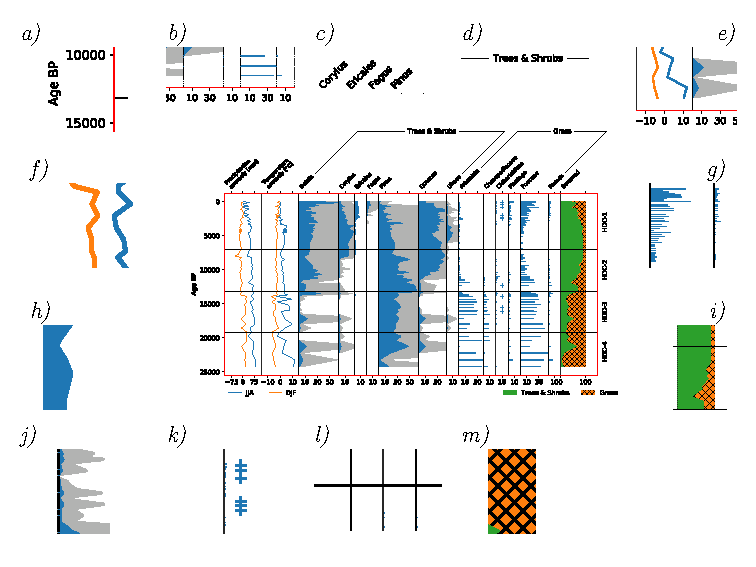
\includegraphics[width=\linewidth]{straditize-figures/sample-diagram-explained.pdf}
	\caption[Common features in a pollen diagram]{Common features in a pollen diagram. The center of the image is a pollen diagram with the data part being highlighted in red, the surrounding subfigures show some of it’s special aspects.
		Subfigures a) – e) show common features in the diagram structure, subfigures f) – i) the different plotting styles and j) – m) some of the special features. \\
		Each variable shares the same vertical axis a), is plotted as one column (sub diagram) marked by a separate vertical line b) and has a rotated title with the name of the variable c). The variables are grouped together d) and potentially have differing units on the horizontal axis  e). Common plotting styles are line diagrams f), bar diagrams g), stacked diagrams h), or  most commonly for pollen, as filled area diagram i). They may also be enhanced through exaggerations j), the visualization of taxon occurences k), horizontal lines as subdivisions of the core and vertical lines as y-axes for the columns l)  and with hatches on the area plots     for visual distinction m).
	}
	\label{fig:sample-diagram}
\end{figure}

In this section we describe the common features of a stratigraphic pollen diagram and their handling within \emph{straditize}. The emphasis is on pollen diagrams
A pollen diagram highlighting the features in a stratigraphic diagram is provided in figure
\ref{fig:sample-diagram}.

\subsection{Structure of a stratigraphic diagram}  \label{sec:straditize-structure}

\subsubsection{Stratigraphic columns}  \label{sec:straditize-strati-columns}
A stratigraphic diagram consists of multiple sub diagrams, each visualizing one or more different variables, for example the percentages of different pollen taxa, the concentration of different chemical elements, or the various percentages of different grain sizes. These sub diagrams share one common axis which is usually the age or depth of the core (see fig.\DIFaddbegin \DIFadd{~}\DIFaddend \samplediagram[a]). 
The diagram is then divided into multiple sub diagrams which we refer to as the columns of the stratigraphic diagram (fig. \samplediagram[b]). Each column visualizes the data of one variable, such as a pollen taxon, or multiple variables where these are plotted within the same column (same x-axis), such as winter and summer precipitation shown in the left most column of figure \samplediagram. The current version of \emph{straditize} requires that the columns do not overlap and that multiple variables plotted in the same column do not overlap either. The software can process multiple variables in a column so long as these are stacked or additive, and therefore they never overlap. An example in a pollen diagram could be where multiple species of, for instance Betula, are plotted as a stacked diagram in a single column so that the sum of the species also shows the total Betula.  

At the top of each column it is usual to find the name of the variable plotted in the column. This may be shown at a variety of angles, but usually either vertically, or at an angle or rotated to make it easier to read and fit within the diagram (fig. \samplediagram[c]). This label can be automatically read by \emph{straditize} and the name assigned to the respective column data, although care should be taken as the label is sometimes offset from the column it represents.  

Variables are also often grouped together and the group labelled, for instance in pollen diagrams into \emph{trees \& shrubs}, and \emph{herbs} (fig.\samplediagram[d]). For pollen data these groups usually share the same x-axis units/scaling (as in fig.\samplediagram[b]). In \emph{straditize} the units/scaling can be set and applied to a whole group of columns/variables, or set and assigned for each individual column/variable (see fig.\samplediagram[e]).

\subsubsection{Diagram types}  \label{sec:straditize-types}
A number of different diagram types are shown in figure \samplediagram\DIFaddbegin \DIFadd{\, }\DIFaddend that are commonly used in pollen diagrams, as well as other stratigraphic diagrams. These can all be identified and read by \emph{straditize}. One of the most commonly found diagrams in pollen diagrams are line diagrams (fig.\samplediagram[f]), or line diagrams where the area underneath of the line is filled to make an area diagram (fig.\samplediagram[h]). Data is also often commonly presented as bar diagrams that make it clearer where the individual samples are located (fig.\samplediagram[g]). Both bar and line/area diagrams may also be stacked, where (as we have already mentioned) columns may contain multiple variables stacked one upon the other (fig.\samplediagram[i]). These various diagram types require different digitization strategies, which we discuss in the digitization section below (see section \ref{sec:straditize-digitization}).

\subsubsection{Informative features}  \label{sec:straditize-features}
Other more specialized features can also be found in pollen diagrams that provide additional information for the reader, but are more difficult to interpret for the software. For instance the taxa or variables in a pollen diagram are usually all plotted on the same scale even if they are in different columns, so that direct visual comparison can be made between them. However, whilst this works well for large percentage values, it can often be difficult to see changes in low percentage values, which may still be ecologically important. To help the reader see these changes in low percentages, pollen diagrams often include a vertical exaggeration. This means that the percentages for a pollen taxa in a column will be plotted with two lines, one showing the percentage value shown on the scale, and the other showing the percentage value multiplied or exaggerated by a certain factor (usually 5 or 10) (fig. \samplediagram[j]). A different approach to the same problem is to mark the low percentages with a symbol or marker. For instance, a common method is to mark all samples with less than 0.5\% or 1.0\% with a \enquote{+} symbol (fig. \samplediagram[k]).

Other features that are often added to pollen diagrams and other stratigraphic diagrams are vertical and horizontal lines. Vertical lines often denote the start of a column, representing the baseline of the y-axes. These are often a continuous or discontinuous dashed line, and when it is quite a thick line it can be difficult to define its position relative to the x-axis. Horizontal lines usually run across columns and are often used to denote different sections of the diagram. For instance, in pollen diagrams they are often used to denote zones or sections of the diagram that have a similar ecological assemblage. These horizontal lines do not usually provide useful numerical data and their intersection with column lines can make reading the column lines more difficult for the software. Another difficulty are hatch patterns which are especially common in old monochrome diagrams that predate the use of shading (fig. \samplediagram[m]). 


\subsection{Digitization procedure}  \label{sec:straditize-digitization}
\emph{Straditize} digitizes the multiple columns or curves within a diagram in a single but editable action. This is different from other digitization software that usually requires the user to digitize each curve individually. This makes the digitization of a diagram with many columns much faster, and at the same time it enables the software to use all of the information in all of the different columns to help infer knowledge common to all columns, such as sample depths and percentage values (see section \ref{sec:straditize-samples}). This all-in-one digitization strategy however requires that \emph{straditize} is able to understand and capture the structure of the diagram without encountering too many interpretation problems. Hence, instead of selecting the features that should be digitized, \emph{straditize} first requires the user to remove all of the features that should not be digitized.

In summary, the digitization procedure for a stratigraphic diagram using \emph{straditize} follows the following steps:

\begin{enumerate}
	\item Define the data part of the diagram
	\item Identify the columns representing the different variables
	\item Clean-up the diagram by removing any unnecessary informative features (see section \ref{sec:straditize-cleaning}) 
	\item Decide how to handling exaggerations and rare occurrences
	\item Digitize the diagram
	\item Identify the samples
	\item Translate the data into the correct x- and y-units
	\item Read in the variable names
\end{enumerate}

All of these steps are semi-automated and the results can (and should) be checked and edited by the user. Each step is fully reversible and the digitization process can be interrupted, saved and reopened at any time. In the following subsections we describe the algorithms of the different steps.

\begingroup
% change the title format of subsubsections to get just the number
\titleformat{\subsubsection}
{\normalfont\normalsize\bfseries}{(\arabic{subsubsection})}{1em}{}

\subsubsection{Defining the data part of the diagram}  \label{sec:straditize-data-part}
The data part (see the red rectangle in fig. \samplediagram), displays the data of the diagram.  Defining this part properly in the diagram image helps \emph{straditize} to identify the part of the diagram from which data is to be extracted. Ideally it should not contain any labels for the horizontal or vertical axes, or any column headers or titles. If this cannot be avoided, these parts will have to be removed afterwards (see section \ref{sec:straditize-cleaning}).

\emph{Straditize} uses a simple procedure to automatically detect the data part of the diagram. It looks for the two outer most pixel rows/columns that cover a certain fraction of the entire image (by default 70\%). This algorithm works if the data part of the diagram is enclosed by a rectangle, as is shown in figure \samplediagram. If there is no rectangle enclosing the data then the user has to define the rectangle.

The data part is then transformed into a binary (black-and-white) version of the diagram image, and all of the informative features need to be removed. In the end, only data pixels, i.e. meaningful pixels that represent the numerical data behind the diagram, should be left (see the following section \ref{sec:straditize-cleaning} and figure \ref{fig:cleaned-sample}).

\subsubsection{Separating the columns}  \label{sec:straditize-columns}

The next important aspect of the diagram structure that needs to be defined are the start of each of the columns (see section \ref{sec:straditize-strati-columns}). This information is particularly important because a small error in each column can quickly sum up when digitizing a diagram with multiple columns. For instance, an error of one pixel in defining the start of every column in a pollen diagram that is about 1400 pixels wide and has 27 taxa is equivalent to an error of about 0.5 percent per taxon. In total this can easily introduce a summed error of up to 12\% per sample. 
\emph{Straditize} uses several criteria to detect the various columns. The start of each column is detected using the following procedure. Let $D(i)$ be the number of data pixels in a pixel column $i$ (see black areas in \ref{fig:cleaned-sample}. Then we assume a column start at pixel column $i$ if

\begin{enumerate}
	\item the previous pixel column $i-1$ did not contain any data ($D(i-1) = 0$)
	\item the amount of data points doubled compared to $i-1$ ($D(i) \geq 2\cdot D(i-1)$)
	\item the amount of data points steadily increases within the next few columns to a value twice as large as the previous column ($D(i+n) \geq 2\cdot D(i-1)$ with $n>0$ and $D(i+j) \geq D(i)$ for all $0 < j \geq n$)
\end{enumerate}

Additionally, the start of each potential column has to contain a user defined number of data pixels, which is by default ten percent of the height of the area containing the data within the diagram (the red rectangle in figure \samplediagram).

\subsubsection{Cleaning up the diagram}  \label{sec:straditize-cleaning}

\begin{figure}
	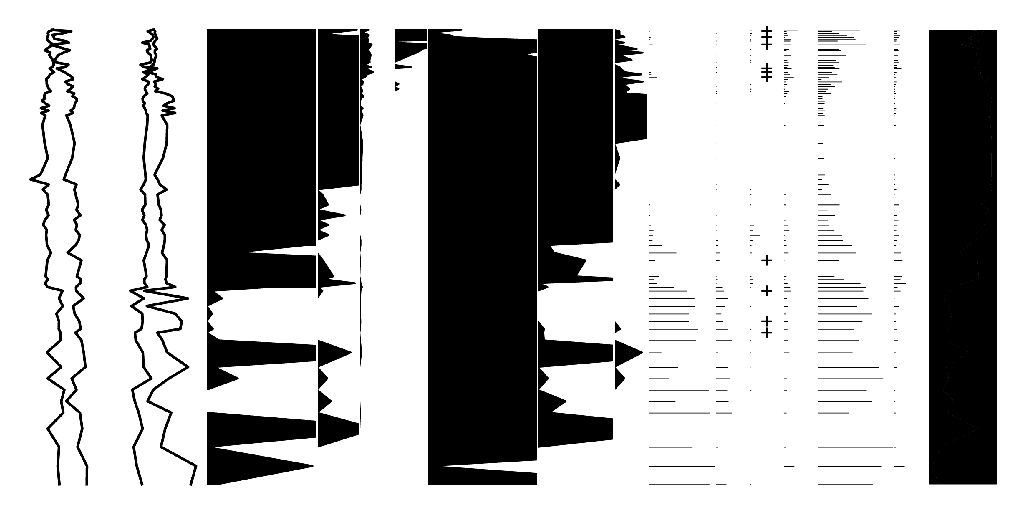
\includegraphics[width=\linewidth]{straditize-figures/sample-diagram-data.pdf}
	\caption[Cleaned binary image of the data part]{Cleaned binary image of the data part of figure \ref{fig:sample-diagram}. Informative features (Y-axes and horizontal lines) have been removed. Exaggerations and occurrences are still in the binary image and are considered separately in section \ref{sec:occurences}.}
	\label{fig:cleaned-sample}
\end{figure}

In order for the automated digitization algorithms to work effectively, \emph{straditize} has to know which pixels contain data (i.e. is part of a line, or a bar), and which pixels are purely informative (such as y-axes or horizontal lines, see fig. \samplediagram[l]). It is necessary for the user to remove informative features from the data part of the diagram to get a clean version that will not confuse the algorithm. Figure \ref{fig:cleaned-sample} shows what this looks like for the sample diagram in figure \samplediagram. \emph{Straditize} has multiple tools to facilitate the removing of informative features, documented in the software and manual, but their applicability depends on the diagram that is subject to digitization.

The most important step of cleaning the diagram is the recognition of the vertical axes (y- axes) that are usually at the start of every column. This is important because it defines the start of the x-axis, and therefore the value assigned to each of the data points, but also because in some cases the line can obscure part of the data itself. For instance, it is possible that the lowest values on the x-axis (see section \ref{sec:straditize-occurences}) are obscured by the vertical line marking the y-axis, making accurate digitization difficult.

\emph{Straditize} therefore has an automatic algorithm to detect vertical axes that tries to minimize the removing of real data pixels. This detection is described by the following algorithm:

Let $C(i)$ be the most frequent color in the pixels of a pixel column $i$, and $D(i)$ the amount of data pixels in this column. A pixel column that is covered by data with more than a user-defined threshold (by default 30 percent of the data part height, see section \ref{sec:straditize-data-part}) is considered as part of a y-axis if 
\begin{itemize}
	\item it is either the first pixel column in the subdiagram with data (i.e. $D(j) = 0$ for $j < i$ and $j$ being larger or equal than the column start of the diagram),
	\item or the dominant color of the pixel column is the same as for the previous pixel column (i.e. $C(i) = C(i-1)$) and the number of data points is approximately the same (i.e. $D(i) \approx  D(i-1)$).
\end{itemize}

This procedure results in one vertical line per column and works independent of whether it is a dotted, dashed or solid line. However, the line width is critical and may vary a lot. If a diagram column contains a filled line (fig. \samplediagram[h]) that merges with the vertical line defining the y-axis, then the algorithm could potentially overestimate the width of the y-axis line. Therefore, we use the median of all of the estimated lines from the various columns as the width of the y-axis line, and reduce the width of each of the lines to this amount.
The algorithm then looks for informative features or other features that appear to be part of the data columns but are not part of the data behind the image. These include small features such as axis tick marks for example, and lighter pixels (i.e. close to white) that are usually a result from the rasterization of the diagram image.
\emph{straditize} then moves the start of the column because it assumes that the starting point for the x-axis (for pollen taxa it would be the 0\% line) is in the middle of the vertical line marking the y-axis.


\subsubsection{Handling low taxon values}  \label{sec:straditize-occurences}

One particular feature often associated with pollen diagrams is the use of vertical exaggeration to help visualize changes in low percentages. Ordinarily, low percentages could be viewed better by changing the x-axis scale for the taxa with low percentages, but with pollen data it is also important to be able to make a visual comparison across all of the taxa listed, including those with high pollen percentages. Therefore, a common scale for all taxa is important. The exaggeration (fig. \samplediagram[j]) usually takes the form of a second line outside of the first, usually representing x5 or x10 exaggeration of the scale presented on the x-axis. This line could be expected to have greater precision than the first for any given pixel resolution, but problems emerge when the value of the exaggerated value exceeds the width of the scale on the x-axis, so that the line marking the exaggerated values is truncated at high values above a certain threshold. 
Another common way to help the reader identify low percentages in pollen diagrams is to use a marker (often a \enquote{+} symbol, fig. \samplediagram[k]) for values below a certain threshold. This can be particularly useful for very low counts where the author wants the reader to be aware that pollen of a certain taxa was found, even if the pollen counted was very low. This is often used for instance with \enquote{important} taxa such as Cereals that can indicate human agricultural activity, and taxa like Larix (Larch) that have notoriously low pollen productivity and where <1.0\% in a pollen diagram may actually represent 20\% of Larix trees in the surrounding landscape. 
For the purpose of digitization, the \emph{straditize} user can either remove these exaggerations, or use some of the functions available in \emph{straditize} to consider both the non-exaggerated and the exaggerated information in the diagram. In the case of the use of symbols to represent values below a threshold, it needs to be decided what value the symbol will represent once it is digitized and turned into numerical data.  In any case, exaggerations and occurences are automatically removed from the image before the diagram is digitized (see next step \ref{sec:straditize-digitize}).

\subsubsection{Digitizing the diagram}  \label{sec:straditize-digitize}

\begin{figure}
	\centering
	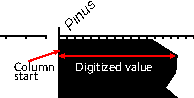
\includegraphics[width=0.5\linewidth]{straditize-figures/sample_diagram_digitize-explanation.pdf}
	\caption[Illustration of the basic digitization strategy of \emph{straditize}]{Illustration of the basic digitization strategy of \emph{straditize}. For each diagram column in the binary image (fig. \ref{fig:cleaned-sample}), we use the pixel that is located furthest to the right on the curve and take the distance to the column start as the digitized value. This is then transformed from the pixel scale into the data units based on the user input.}
	\label{fig:digitize-explanation}
\end{figure}

After removing the informative features (see section \ref{sec:straditize-cleaning}) and exaggerations (see section \ref{sec:straditize-occurences}), \emph{straditize} can automatically digitize the various columns on a pixel basis. In general \emph{straditize} treats every column of the diagram separately and uses different algorithms for the various plotting types:

\begin{description}
	\item[Area and line diagrams] such as those shown in the fig. \samplediagram[f] and fig. \samplediagram[h]  are  digitized  based  on  the  pixel located furthest to the right on the curve in any particular column (illustrated in figure \ref{fig:digitize-explanation}).
	\item[Bar diagrams] as in figure \samplediagram[g] are also digitized based on the the pixel located furthest to the right on the bar in any particular column. Additionally, \emph{straditize} distinguishes between two adjacent bars by using a user defined threshold (by default two pixels). Additionally, it identifies bars that are significantly wider than the others (which would indicate two or more overlapping bars) and then the user can split them manually.
	\item[Stacked diagrams] as in figure \samplediagram[i] have to be digitized manually. The user has to manually distinguish the different areas using the selection tools in \emph{straditize}.
\end{description}

These procedures each result in one value per pixel row in each variable column in the data part. The next step is then to extract only the rows that are necessary to regenerate the diagram, that is, the pixel rows that correspond to the samples.

\subsubsection{Finding the samples}  \label{sec:straditize-samples}
A key function of \emph{straditize} is its ability to identify sample levels in the data, so that measurements of x-axis values in each column for each variable are assigned to the appropriate y-axis sample depth or age across all columns and variables. The search and assignment of sample levels can be done either automatically or manually, and if done automatically, this can also be later edited following manual checking.  

The algorithm is thereby split into two steps:

\begin{enumerate}
	\item For each column: Identify the intervals that contain exactly one sample (the rough locations, i.e. certain consecutive pixel rows in every column where we know that there is a sample, but we do not know where exactly) \label{enum:sample-1}
	\item Align the overlapping intervals between the columns to estimate the exact location \label{enum:sample-2}
\end{enumerate}

The implementation of step \ref{enum:sample-1} necessarily differs between 
bar and area/stacked/line diagrams. With bar diagrams \emph{straditize} uses the bars identified in the
previous digitization step (section \ref{sec:straditize-digitize}) to define these rough sample locations, while for the other diagram types the algorithm looks for local extrema in the graph line, i.e. intervals that are lower or higher than the surrounding areas. This implies that each sample is associated with a local minimum or maximum in at least one of the diagram columns. This holds well for pollen diagrams that usually sum up to 100\% across all of the columns or variables in the diagram, but it is however not generally true for all stratigraphic diagrams.

Step \ref{enum:sample-2} then aligns these rough intervals and uses the overlapping information from the different columns to estimate the exact location of the sample. This is described by the following procedure, where we focus on a simple case of only two diagram columns. Assume that the two columns $i$ and $j$ have a sample in the corresponding overlapping intervals $I_i$ and $I_j$ (i.e. $I_i = \left\{r_{i,1}, r_{i,2}, \ldots\right\}$, and $I_j = \left\{r_{j,1}, r_{j,2}, \ldots\right\}$ with $I_i \cap I_j \neq \emptyset$). To find the exact location, \emph{straditize} distinguishes the following cases:

\begin{description}
	\item[If one of the intervals contains only one pixel row] (i.e. $\left| I_i \right| = 1$ or $\left| I_j \right| = 1$), \emph{straditize} sets the sample at exactly this location
	\item[If each of the intervals contains multiple rows,] \emph{straditize} uses the mean of all the row indices in each of the intervals (i.e. $y = \overline{I_i \cup I_j}$). This then weighs overlapping areas in the intervals above non-overlapping areas.
\end{description}

Finally, samples that are close to each other (by default, closer than 5 pixel rows) are merged together. This is necessary because it may happen that, due to the quality of the diagram image, two rough locations do not exactly overlap although they belong to the same sample.


\setcounter{secnumdepth}{2}
\endgroup

\section{Discussion}  \label{sec:straditize-discussion}

\begin{figure}
	\centering
	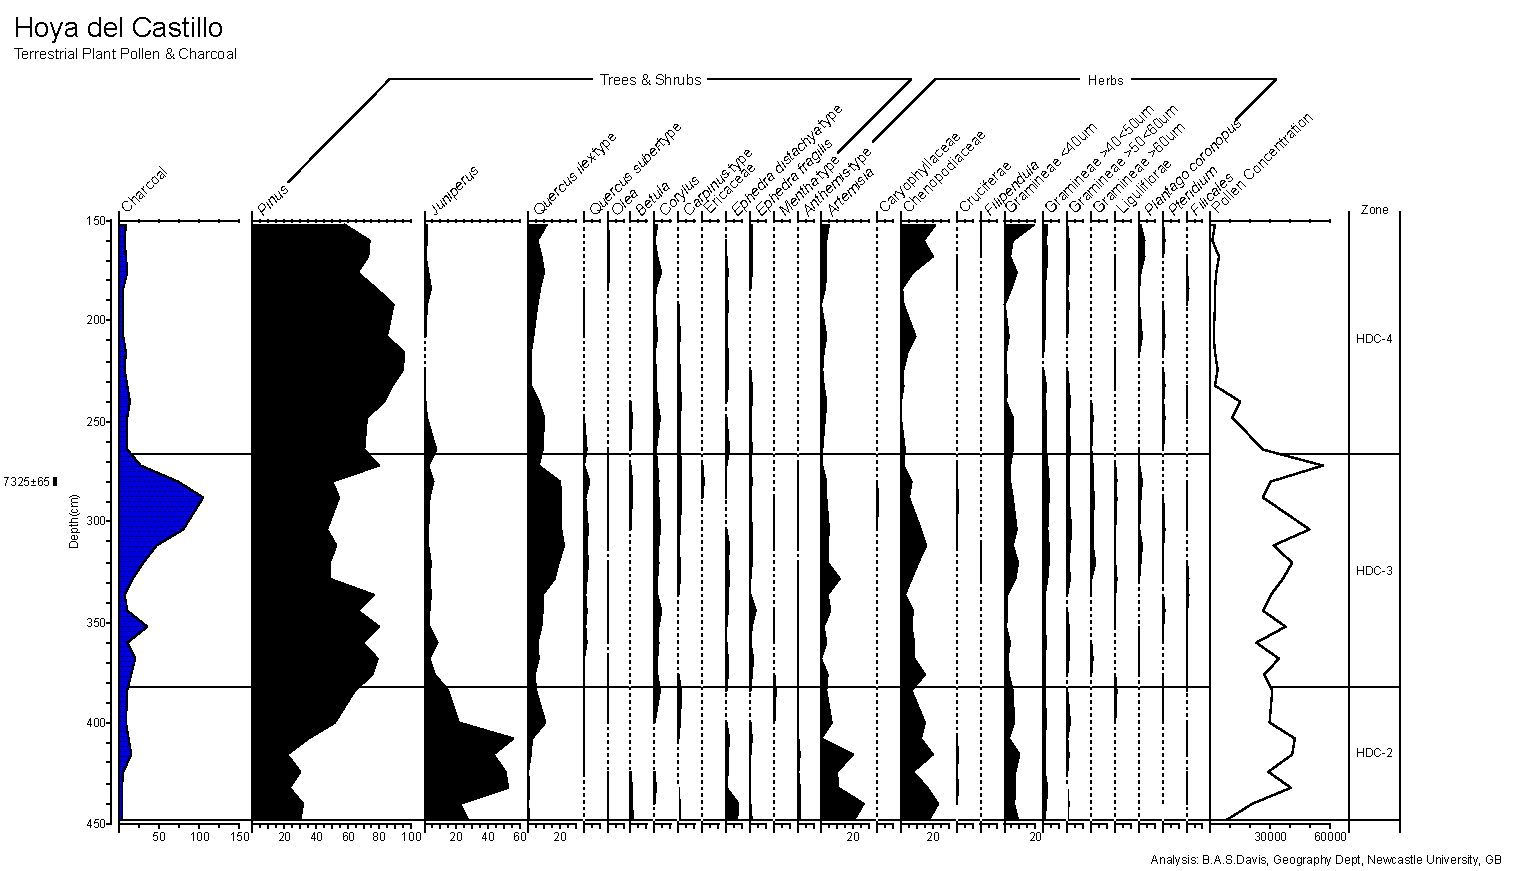
\includegraphics[width=0.45\linewidth]{straditize-figures/hoya-del-castillo.pdf}
	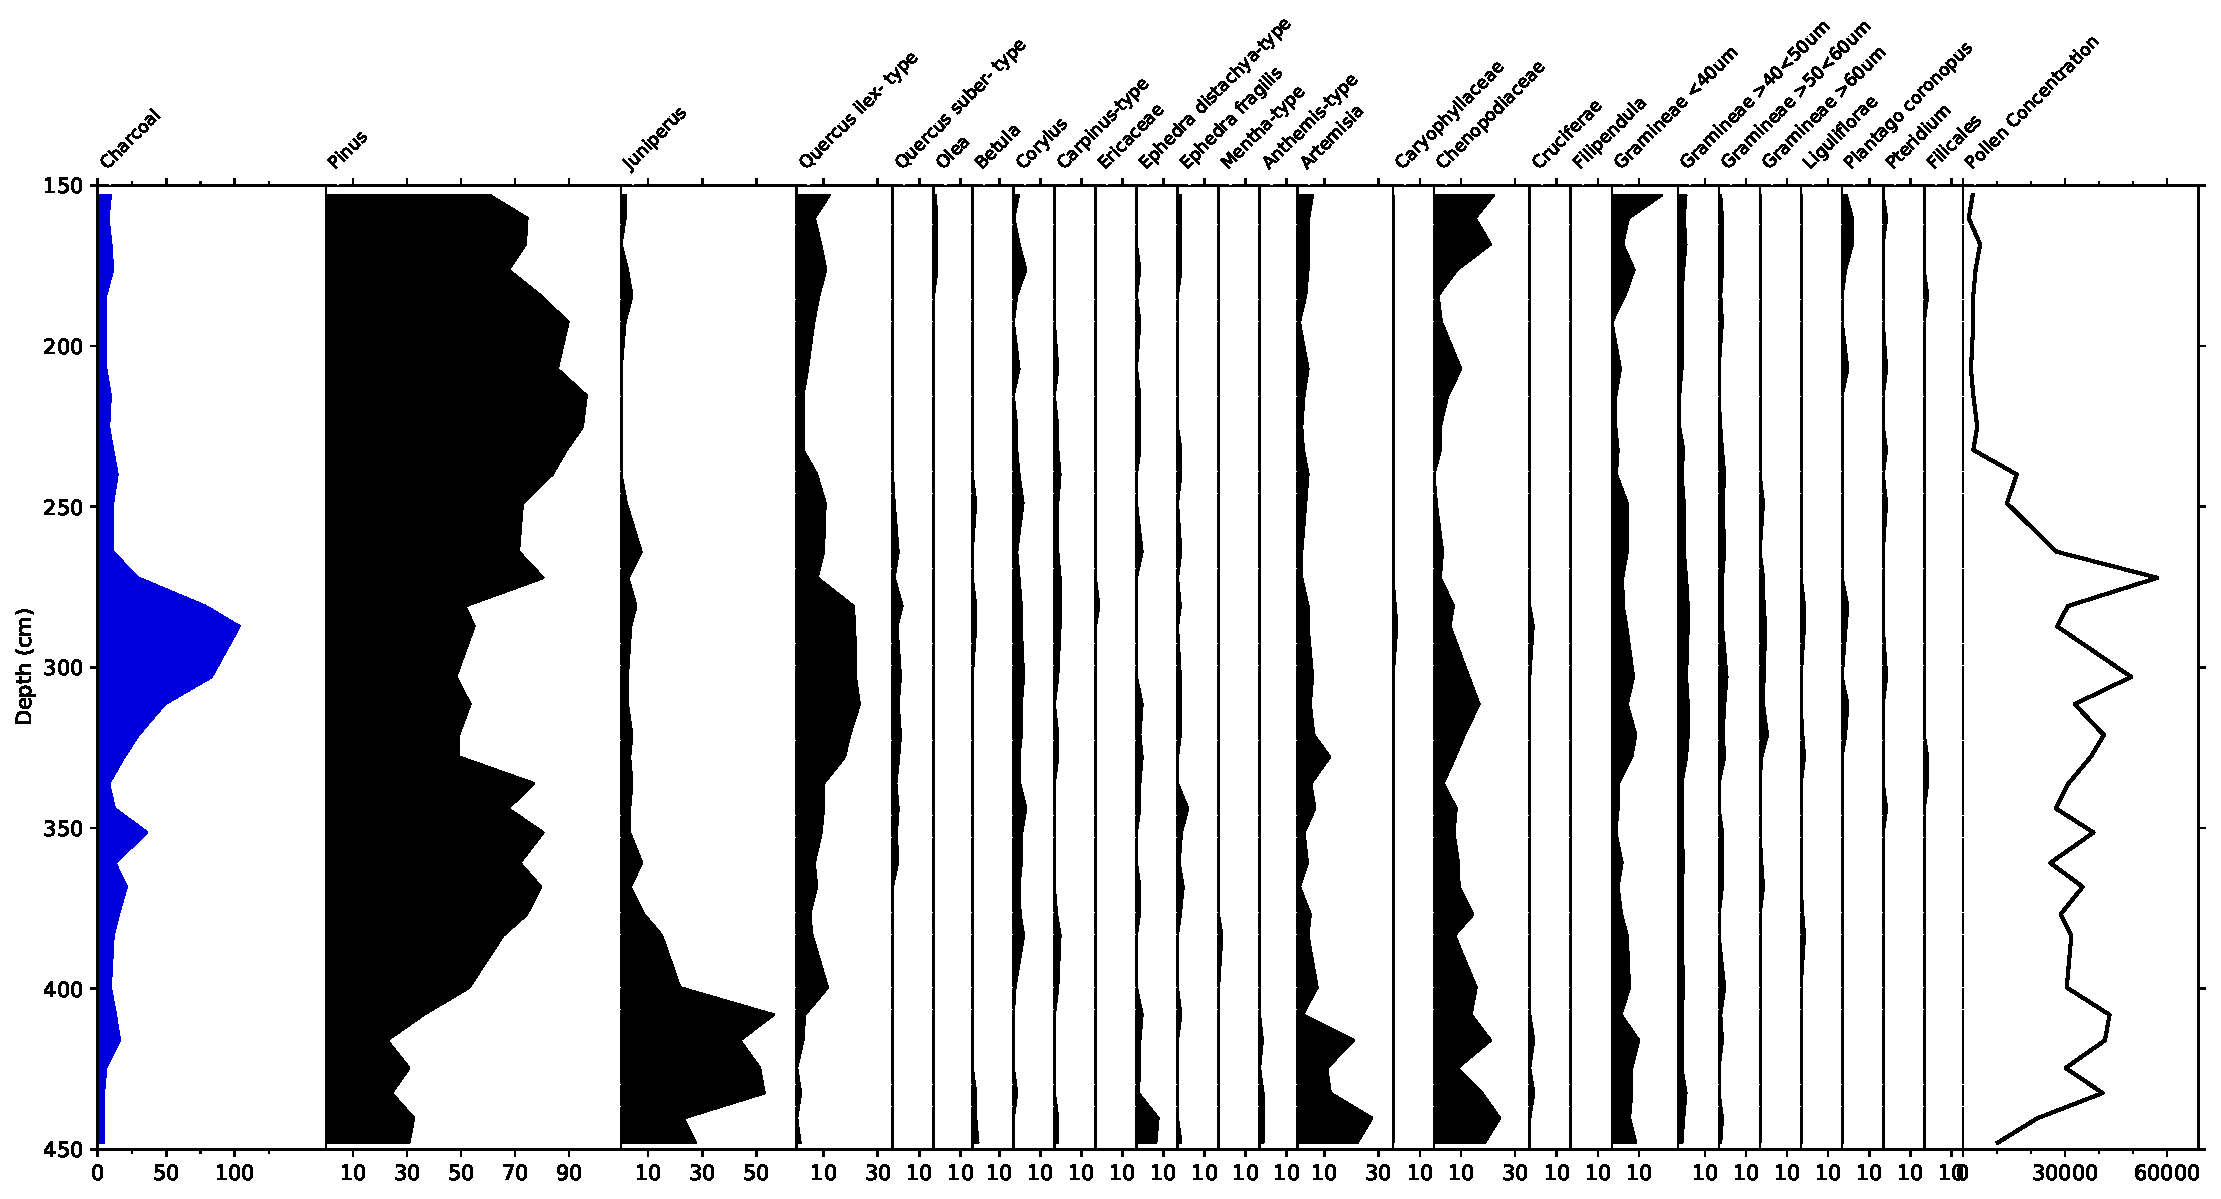
\includegraphics[width=0.45\linewidth]{straditize-figures/hoya-del-castillo-digitized.pdf}
	\caption[Pollen diagram for Hoya del Castillo]{Pollen diagram for Hoya del Castillo after \cite{DavisStevenson2007}. Left,  the original diagram, right, the digitized version obtained (and plotted) using \emph{straditize}.}
	\label{fig:hoya-del-castillo}
\end{figure}

\begin{figure}
	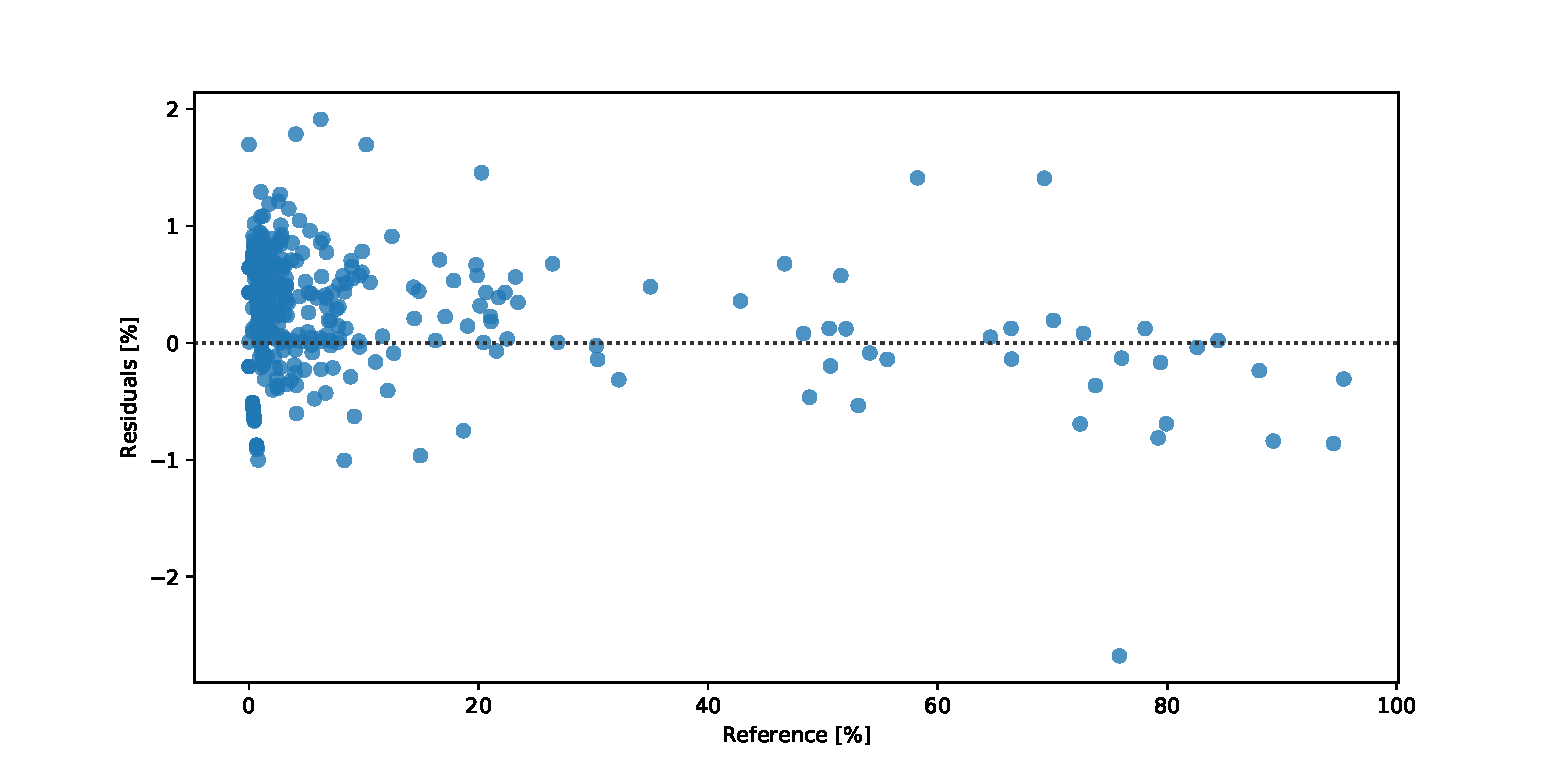
\includegraphics[width=\linewidth]{straditize-figures/resid-plot-hoya-del-castillo.pdf}
	\caption[Residuals plot of the digitized Hoya del Castillo diagram]{A plot of the residuals based on a comparison between the digitized Hoya del Castillo pollen diagram, and the original reference data that was used to generate the diagram (see fig. \ref{fig:hoya-del-castillo}). The y-axis shows the residuals (digitized data percentage minus original reference data percentage) and the x-axis shows the original reference data percentage for Hoya del Castillo. Each dot represents a single pollen sample. The dotted line denotes the one-to-one line where digitization result and reference are the same.}
	\label{fig:hoya-resid}
\end{figure}

As an example of the application of \emph{straditize}, we digitized the Holocene pollen diagram for Hoya del Castillo (Spain) a site in Los Monegros, NE Spain, published by \cite{DavisStevenson2007} (see figure \ref{fig:hoya-del-castillo}). The diagram was generated using the popular pollen diagram plotting software package Tilia\footnote{\url{https://www.tiliait.com/}} \citep{Grimm1988, Grimm1991} and exported as an image with a resolution of 450 dots per inch (dpi). We then followed the strategy described in section \ref{sec:straditize-digitization} to digitize the diagram. First, we selected the data part, then the columns and cleaned the image by removing the y-axes and horizontal lines. Then we digitized the diagram and used the \emph{straditize} sample finding algorithm to extract the sample locations.  

Comparing the digitized data with the original data, we find that \emph{straditize} was able to successfully identify all 34 samples in the diagram. The root mean square error (RMSE) for the depth of each sample digitized from the y-axis and normalized by the range of the vertical axes, is very low and corresponds to an error of 0.2\%. Additionally \emph{straditize} gives a good measure of the individual taxon percentage with the RMSE being only 0.5\%. Nevertheless, \emph{straditize} shows a tendency to overestimate the real percentage. About 43\% of the samples have percentages that are higher than the orginal percentages, whereas only about 10\% have lower percentages (fig. \ref{fig:hoya-resid}), the remainder are exact (and most of the time zero percentage). This is probably due to a systematic bias in the positioning of the exact column start, i.e. 0 start point of the x-axis relative to y-axis baseline, and is something that could be systematically corrected. Overall this error is in the range of less than one percent per sample/taxon.

Irrespective of the performance of the software, other factors will also influence the accuracy of the digitization process. The quality and type of diagram image is very important, especially if the diagram is not of a high pixel resolution, or has poorly aligned and marked axis, or has many closely located samples. But also the skill and experience of the user will have some impact, especially if they are also unfamiliar with the type of data being analyzed and the way that it is commonly presented in a diagram. To help the user evaluate how accurate the digitization process has been, \emph{straditize} also allows the user to plot the digitized data in a way that allows a direct visual comparison with the source diagram (fig. \ref{fig:hoya-del-castillo}) using the stratigraphic visualization features of \textit{psy-strat} \citep{Sommer2019}.

Keeping in mind these many caveats, we generally estimate that \emph{straditize} will allow an experienced user to reliably obtain a numerical estimate through diagram digitization in the order of 1\% of the original data for each sample/variable. In the case of pollen diagrams, this uncertainty should be viewed from the perspective of the inherent uncertainty associated with the counting of each pollen sample. Any pollen count is an estimate of the pollen sample that is displayed on a pollen slide. Although pollen samples are usually displayed as percentages, the reason for this is that the size of the pollen count varies from sample to sample, and percentages allow different samples to be directly compared on a common scale. Each count is a sample of the total pollen assemblage on a slide, and therefore each count represents an estimate of the composition of the total pollen assemblage represented on the slide. The more of that pollen assemblage that is counted, the closer that estimate will be to the actual pollen assemblage. This mean that each pollen sample plotted on a pollen diagram has an inherent uncertainty that is related to the total number of pollen grains counted. The bigger the count, the lower the uncertainty. Typical 0.95 confidence intervals for individual taxa based on a typical pollen count of around 300-500 pollen grains are easily in the order of 2-5\% \citep{Maher1972}.

\section{Conclusions}  \label{sec:straditize-conclusions}
In this paper we present a new open-source software that is capable of greatly reducing the time required to accurately digitize stratigraphic diagrams. These diagrams are characterized by a series of horizontally or vertically aligned diagrams that plot various variables representing the results of the analysis of a series of common samples that are aligned on the same y-axis representing age or depth. The software is currently optimized for use with pollen diagrams, but should work well with any similar type of data plotted in a similar style. The x-axis values can be percentages or absolute values of any kind, and the y-axis could also represent distance down a river of any other linear scale. The program is freely available, well documented with integrated help and training, is written in python, and is also open for adaptation for other uses. 

\printbibliography[heading=subbibintoc]

\end{refsection}
% psyplot chapter

\Chapter{Psyplot}{A flexible framework for interactive data analysis}

\label{chp:psyplot}

\begin{refsection}

%----------------------------------------------------------------------------------------
%	SECTION 1
%----------------------------------------------------------------------------------------

\section{Summary}  \label{sec:psyplot-joss}

\blockquote{
	\textit{From}
	\bibforkey{Sommer2017}
}

\noindent psyplot \citep{Sommer2017} is a cross-platform open source python project that mainly combines the plotting utilities of matplotlib \citep{Hunter2007} and the data management of the xarray \citep{HoyerHamman2017} package and integrates them into a software that can be used via command-line and via a \glsfirst{gui}.

The main purpose is to have a framework that allows a fast, attractive, flexible, easily applicable, easily reproducible and especially an interactive visualization of data.

The ultimate goal is to help scientists in their daily work by providing a flexible visualization tool that can be enhanced by their own visualization scripts.

The framework is extended by multiple plugins: psy-simple \citep{Sommer2017b} for simple visualization tasks, psy-maps \citep{Sommer2017c} for georeferenced data visualization and psy-reg \citep{Sommer2017d} for the visualization of fits. It is furthermore extended by the optional graphical user interface psyplot-gui \citep{Sommer2017e}.


\section{Introduction}  \label{sec:psyplot-review}

The mathematical and statistical processing of climate data is closely related to its visualization and analysis. But in traditional visual analytics literature, these two aspects are commonly treated in separate manners. \cite{KeimAndrienkoFeketeEtAl2008} for instance, (following \cite{Wijk2005}) distinguish two steps of visual analytics, the initial data processing with statistical or mathematical techniques, and a \textit{sense-making loop} of visualization, exploration and the gain of new knowledge. \cite{BoettingerRoeber2019} distinguish the \textit{filtering} step (data processing), and \textit{mapping}/\textit{rendering} step that describes the visualization. Also in the literature there is a clear division between the climate visualization (or visual analytic) papers and the standard statistical or climate literature that describes new methods for data processing. Visualization research focuses mainly on advanced visualization tools such as ParaView \citep{Ayachit2015}, VAPOR \citep{ClyneMininniNortonEtAl2007} or Avizo\footnote{\url{https://www.fei.com/
software/avizo3d/}} \citep[e.g.][]{RautenhausBoettingerSiemenEtAl2018, NockeBuschmannDongesEtAl2015, WongShenLeungEtAl2014, BoettingerRoeber2019} whereas statistical or climate literature commonly uses R \citep{RCT2019}, Python \citep{Oliphant2006, PerezGrangerHunter2011}, \glspl{cdo} \citep{Schulzweida2019} or other command-line tools.

This separation, however, devalues the interplay between the new knowledge from the visualization step, that commonly raises the need for more statistical and mathematical processing of the initial data. This calls for integrated and flexible tools that tackle both steps: the data processing and the visualization, a requirement that is currently not fulfilled by the visualization tools described above. An example software that integrates data processing and data visualization is provided with the Earth System Model Evaluation Tool (ESMValTool) \citep{EyringRighiLauerEtAl2016}. This framework provides common diagnostics for \glspl{esm} to enable model intercomparisons. The tool, however, has limited interactivity and a slow learning curve for the implementation of new diagnostics.

This lack leads to large efforts of climate scientists to develop scripts for the data processing and visualization. They usually do not follow a systematic framework and as such need to be adapted every time a new project starts which also make them difficult to share with other researchers. The new \textit{psyplot} framework wants to generalize this data processing and visualization by providing a framework that is highly flexible, interoperates with standard computational data processing tools and enables flexible visualizations and adaptations. The software is written in the programming language Python \citep{PerezGrangerHunter2011} and builds upon the visualization package \textit{matplotlib} \citep{Hunter2007} and the N-dimensional array processing package \textit{xarray} \citep{HoyerHamman2017}, that closely interoperates with the numeric packages numpy and scipy \citep{JonesOliphantPetersonEtAl2001, Oliphant2006} and the parallel computing library dask \citep{DDT2016}. Due to the flexibility of Python, it can be used from the command-line, a \gls{gui} (section \ref{sec:psyplot-gui}) or jupyter notebooks\footnote{\url{https://jupyter.org/}} \citep{KluyverRaganKelleyPerezEtAl2016}. As such, it supports out-of-core computation (i.e. the processing of data too large to fit into memory), a rich set of visualization methods from matplotlib, and can be extended to other visualization packages, such as the 3D-visualization framework VTK \citep{Sommer2019a}.

The next section \ref{sec:psyplot-framework} provide an overview of the framework with \DIFdelbegin \DIFdel{it's }\DIFdelend \DIFaddbegin \DIFadd{its }\DIFaddend data model, plugins and \gls{gui}. Sections \ref{sec:psyplot-conclusions} and \ref{sec:psyplot-outlook} finally discuss further usage and extensions to the software. For more information, usage and implementation examples I also refer to the online documentation \url{https://psyplot.readthedocs.io}.

\section{The psyplot framework}  \label{sec:psyplot-framework}

The psyplot framework consists of three parts: The core structure that is built upon \textit{xarray} and provides the general infrastructure (section \ref{sec:psyplot-model}), the plugins that use the plotting functionalities of \textit{matplotlib} (section \ref{sec:psyplot-plugins}), and the \gls{gui} (section \ref{sec:psyplot-gui}).


\subsection{Data model}  \label{sec:psyplot-model}

\subsubsection{Psyplot and xarray}  \label{sec:psyplot-dependencies}

psyplot acts as a high-level interface into the packages \textit{xarray} and \textit{matplotlib}. The first one is a recent package for N-dimensional labeled arrays that adopts Unidata’s self-describing Common Data Model on which the network Common Data Form (netCDF) is built \citep{RewDavis1990, BrownFolkGoucherEtAl1993, HoyerHamman2017}. The package integrates with standard python from the python environment, such as the computing and analysis packages numpy \citep{Oliphant2006}, scipy \citep{JonesOliphantPetersonEtAl2001, Oliphant2007}, pandas \citep{McKinney2010} and statsmodels \citep{SeaboldPerktold2010}, but also offers intuitive interfaces for other packages, such as a package for empirical orthogonal functions \citep[EOFs, ][]{Dawson2016}, \glspl{cdo} \citep{Mueller2019}, fourier transforms \citep{UchidaRokemNicholasEtAl2019} \DIFdelbegin \DIFdel{any }\DIFdelend \DIFaddbegin \DIFadd{and }\DIFaddend many more\footnote{\label{foot:xraccessors} several packages related to xarray are listed in the docs at \url{http://xarray.pydata.org/en/stable/related-projects.html} and psyplots integration (accessors) in particular is shown at \url{https://psyplot.readthedocs.io/en/latest/accessors.html}.}. This large \DIFdelbegin \DIFdel{range of extensibility }\DIFdelend \DIFaddbegin \DIFadd{potential for extension }\DIFaddend distinguishes psyplot from other high-level visualization software, such as ParaView or Vapor, \DIFdelbegin \DIFdel{and they can all }\DIFdelend \DIFaddbegin \DIFadd{as such python packages can }\DIFaddend be implemented as a \DIFdelbegin \DIFdel{formatoption (}\DIFdelend \DIFaddbegin \DIFadd{so-called }\textit{\DIFadd{formatoption}} \DIFadd{(without hyphen, }\DIFaddend see below) or used in a pre-processing step.

\subsubsection{Psyplot core structure}  \label{sec:psyplot-core}  

\begin{figure}
	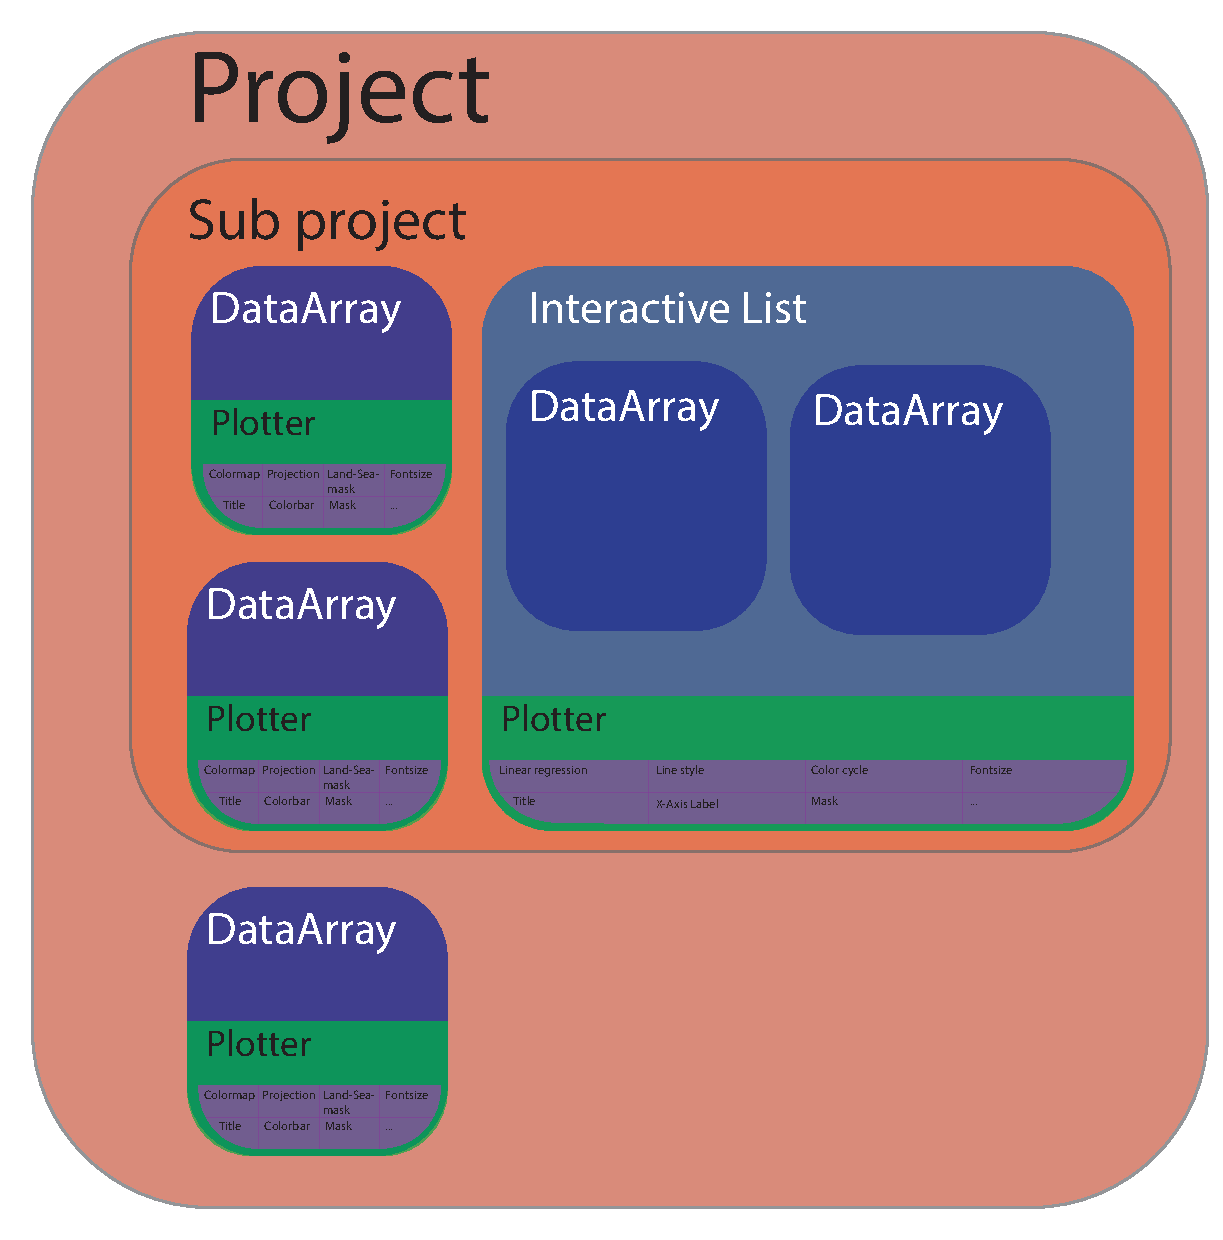
\includegraphics[width=\linewidth]{psyplot-figures/psyplot_framework.pdf}
	\caption[The psyplot core framework]{The psyplot core framework. A (sub) project consists of n-dimensional data arrays or a list of these that are each visualized by a plotter. Each plotter consists of a set of formatoptions that control the appearance of the plot or performs data manipulation.}
	\label{fig:psyplot-core}
\end{figure}

The core structure of psyplot consists of five base classes that interact with each other, the visualization objects \textit{Plotter} and its \textit{Formatoptions}, the data objects \textit{DataArray}, an \textit{InteractiveList} of them, and a collection of all of them, the psyplot \textit{Project}. It is schematically visualized in figure \ref{fig:psyplot-core}.

The most high-level \gls{api} object is the psyplot project that consists of multiple data objects that are (or are not) visualized. The main purpose is a parallel handling of multiple plots/arrays that may also interact with each other (e.g. through the sharing of formatoptions). It mainly spreads update commands to \DIFdelbegin \DIFdel{it's }\DIFdelend \DIFaddbegin \DIFadd{its }\DIFaddend contained objects, but also serves as a filter for the data objects. Furthermore, one project may be split up into sub projects which then only control a specific part of the main project, e.g. for a specific formatting of only a small part of the data.

The next level is the \textit{DataArray} from the xarray package (or more explicitly, \DIFdelbegin \DIFdel{it's }\DIFdelend \DIFaddbegin \DIFadd{its }\DIFaddend accessor, the \textit{InteractiveArray}$^{\ref{foot:xraccessors}}$), that holds the data of one (or more) variables (e.g. temperature) and its corresponding coordinates (e.g. time, latitude, longitude, etc.). It may be one or multidimensional depending on the chosen visualization method. psyplot offers several methods to provide the coordinates for the plotting of different grids to make the visualization easier. The software can \DIFdelbegin \DIFdel{interprete }\DIFdelend \DIFaddbegin \DIFadd{interpret }\DIFaddend CF Conventions\footnote{\url{http://cfconventions.org}} and UGRID conventions for unstructured grids \citep{JagersStuebeGrossEtAl2018}.

Multiple of these arrays can also be grouped together into an \textit{InteractiveList} that shall be visualized by the same plot method (e.g. multiple lines or a scalar field with overlying vector field).

The visualization part in the framework is managed by the \textit{Plotter} class, a collection of multiple \textit{Formatoptions}. Each plotter subclass is designed to visualize the data in a specific manner (e.g. via line plots, violin plots, or map plots) and is completely defined through it’s formatoptions.

\textit{Formatoptions} are the core of the psyplot structure. The standard functionality of a formatoption is to control the visual appearance of one aspect of the plot (e.g. through the colormap, figure title, etc.). It is, however, completely unlimited and can also do data manipulations or calculations. The psy-reg plugin for example (see section \ref{sec:psyplot-plugins}) implements a formatoption that performs a regression through the data that is then visualized. As mentioned earlier, each plotter is set up through \DIFdelbegin \DIFdel{it’s }\DIFdelend \DIFaddbegin \DIFadd{its }\DIFaddend formatoptions where each formatoption has a unique formatoption key inside the plotter. This formatoption key (e.g. \textit{title} or \textit{cmap}) is what is used for updating the plot, manipulating the data, etc.. Formatoptions might also interact with other formatoptions inside the plotter or from other plotters. This concept of formatoptions allows to use the same formatoption with all different kinds of plotters and the interaction of multiple plots with each other. Common plot features, such as the figure title, colormap, etc., therefore \DIFdelbegin \DIFdel{don't }\DIFdelend \DIFaddbegin \DIFadd{do not }\DIFaddend have to be implemented explicitly for every plotter but can be used from existing implementations. This framework also allows a very easy integration and development of own formatoptions with a low or high level of complexity.

\subsection{Psyplot plugins}  \label{sec:psyplot-plugins}

The psyplot package provides the core of the data management described in the previous section \ref{sec:psyplot-model}. The real visualization is implemented in external plugins. The advantage of this approach is an increased flexibility of the entire framework (collaborations can evolve through dedicated plugins) and of managing the various dependencies of the packages. As such, the dependencies of psyplot are rather week (only xarray is needed), but the dependencies of the plugins can be more extensive (e.g. for geo-referencing or advanced statistics). 

Each plugin defines new \textit{Plotters} and \textit{Formatoptions} that are specific to the purpose of the visualization/analysis task. The plotters can also be implemented as a plot method (see supplements \ref{sec:psy-simple-plotmethods} to \ref{sec:psy-strat-plotmethods}) and accessed through the psyplot core \gls{api} (see supplements \ref{sec:psyplot-example} for an example).

The current lists of plugins include \textit{psy-simple} for rather simple and standard visualization tasks, \textit{psy-maps} for geo-referenced plots, \textit{psy-reg} for statistical analysis visualization, and \textit{psy-strat} for stratigraphic diagrams.

\subsubsection{psy-simple: The psyplot plugin for simple visualizations}

Much of the functionality that is used by other plugins is developed in the psy-simple plugin. This package targets simple visualizations and currently includes plot methods for one-dimensional data: line plots, bar plots and violin plots; for two-dimensional data: scalar plots, vector plots and combined scalar and vector plots; and plots that do not require complex data manipulation: a density plot and a plot of the weighted geographic mean. A full list of examples is provided in the supplementary material, section \ref{sec:psy-simple-plotmethods}.

This package also implements most of the functionality to handle unstructured grids in 2D visualizations and defines most of the commonly used formatoptions. The latter include text manipulation (such as plot title, figure title, x- and y-axis labels, etc.), data masking, x- and y-axis tick labeling and positioning, as well as color coding for 2D plots (colormap, colormap sections, etc.).

\subsubsection{psy-maps: The psyplot plugin for visualizations on a map}

psy-maps builds on top of the psy-simple plugin and extends \DIFdelbegin \DIFdel{it's }\DIFdelend \DIFaddbegin \DIFadd{its }\DIFaddend functionality for visualizations on a map using the functionalities of the cartopy package \citep{Cartopy} (see supplements \ref{sec:psy-maps-plotmethods} for examples). It simplifies as such the automated generation of maps for climate model data through the flexibility of the psyplot framework.

psy-maps currently implements additional formatoptions for choosing the projection of the map, selecting the geographic region, drawing the contintens or shaded reliefs of land and ocean, and more. One feature that distinguishes psy-maps from other visualization software, even from pure cartopy, is the ability to visualize unstructured geo-referenced grids on the map. For this purpose, triangles are projected in a pre-processing step to the target projection, prior to the visualization with matplotlib. This drastically increases the performance and makes it possible to visualize even very large data sets. As such, psy-maps visualizes a global scalar field on a hexagonal grid of roughly 4.4 million grid cells ($\approx 13$ km resolution) in roughly 3.5 minutes. The interactive usage of such a large dataset is however limited by the functionalities of matplotlib to handle such an immense amount of data.

\subsubsection{psy-reg: The psyplot plugin for visualizing and calculating regression plots}

psy-reg performs regression analysis on 1D variables using the methods of the statsmodels \citep{SeaboldPerktold2010} and scipy \citep{JonesOliphantPetersonEtAl2001, Oliphant2007} packages, and visualizes the results with the functionalities of the psy-simple plugin. As such, it implements formatoptions for univariate regressions, confidence intervals via bootstrapping, and combined plots of the data density and the fitted model (see also supplements \ref{sec:psy-reg-plotmethods}). The necessity for this package arose from the need to visualize a regression model, compare it (visually) with the original data and to use it afterwards. Other python packages either focus only on the generation of the regressions (such as statsmodels or scipy), or on their visualization (such as seaborn \citep{WaskomBotvinnikOKaneEtAl2018}). The psyplot plugin makes it possible to generate the visualization and to access the underlying regression model parameters and uncertainties.

psy-reg has been heavily used for the parameterization of the weather generator in chapter \ref{chp:gwgen} which also gave the initial motivation for the package. 

\subsubsection{psy-strat: A psyplot plugin for stratigraphic plots}

psy-strat \citep{Sommer2019} is the latest plugin for psyplot that has been developed for stratigraphic diagram visualization. It is particularly designed for the straditize software \citep[chapter \ref{chp:straditize}]{SommerRechChevalierEtAl2019} and was motivated by the need for an automated creation of pollen diagrams. One example of such a diagram is provided in the supplementary material, section \ref{sec:psy-strat-plotmethods}.

As the psy-reg and psy-maps plugins, psy-strat uses the functionalities of the psy-simple plugin for a visualization of multiple variables in separate diagrams that share one common vertical axis (usually age or depth)\footnote{See \href{https://psy-strat.readthedocs.io}{psy-strat.readthedocs.io} for an example of psy-strat.}. Additionally, besides the integration that is common for every psyplot plugin (see next section \ref{sec:psyplot-gui}), psy-strat contains additional functionalities for the psyplot \gls{gui}. This implementation allows the user to select and reorder the variables (pollen taxa) that are shown in the stratigraphic diagram.


\subsection{The psyplot Graphical User Interface}  \label{sec:psyplot-gui}

\begin{figure}
	\begin{tikzpicture}
		\node[anchor=south west,  inner sep=0] (image) at (0,0,0) {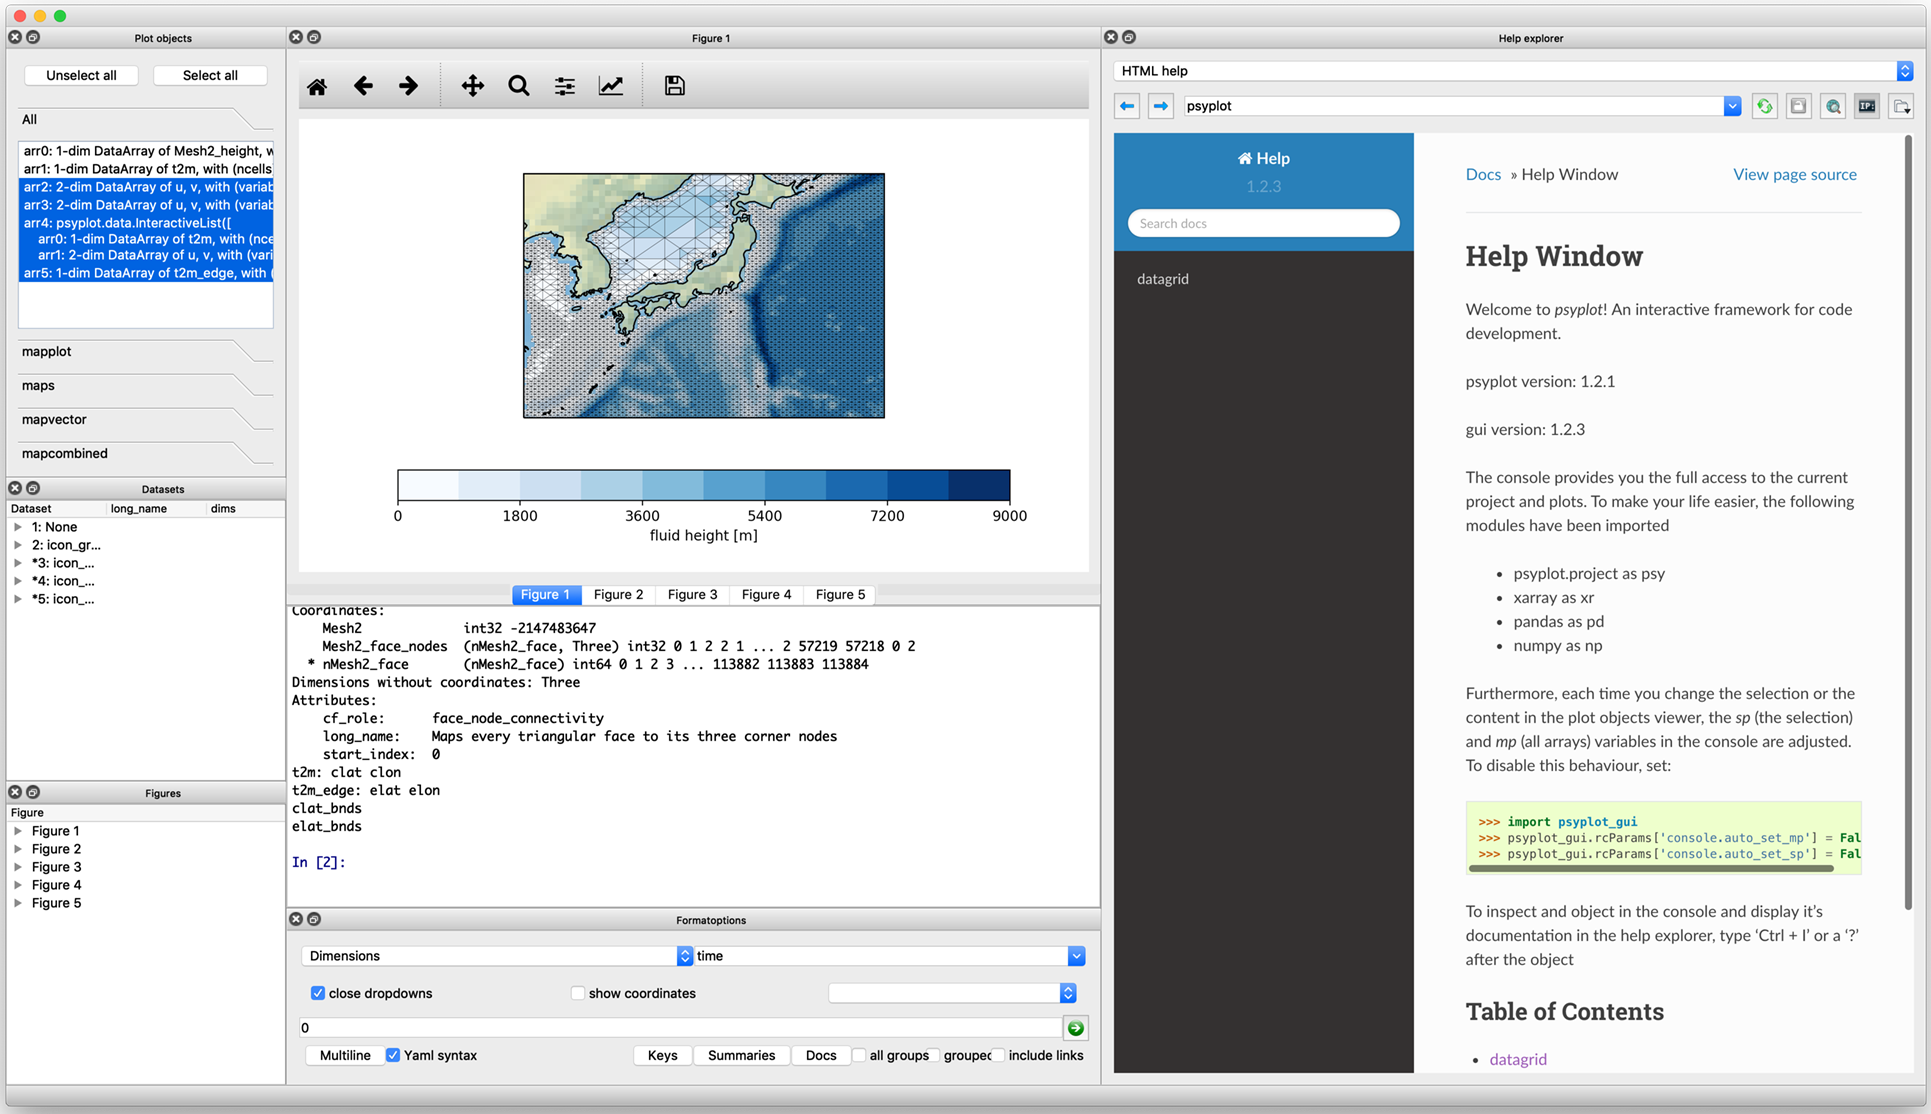
\includegraphics[width=\linewidth]{psyplot-figures/psyplot-gui.png}};
		\node[] (figures) [above=of image, xshift=-0.1\linewidth, yshift=-0.5cm, fill=red!50] {Figures};
		\node (project) [left=of figures, xshift=-0.1\linewidth, fill=red!50] {Project content};
		\node (help) [right=of figures, xshift=0.2\linewidth, fill=red!50] {Help explorer};
		\node (formatoptions) [below=of image, xshift=-0.1\linewidth, yshift=0.5cm, fill=red!50] {Formatoptions};
		\node (console) [above=of formatoptions, yshift=1.5cm, fill=red!50] {Console};
	\end{tikzpicture}
%	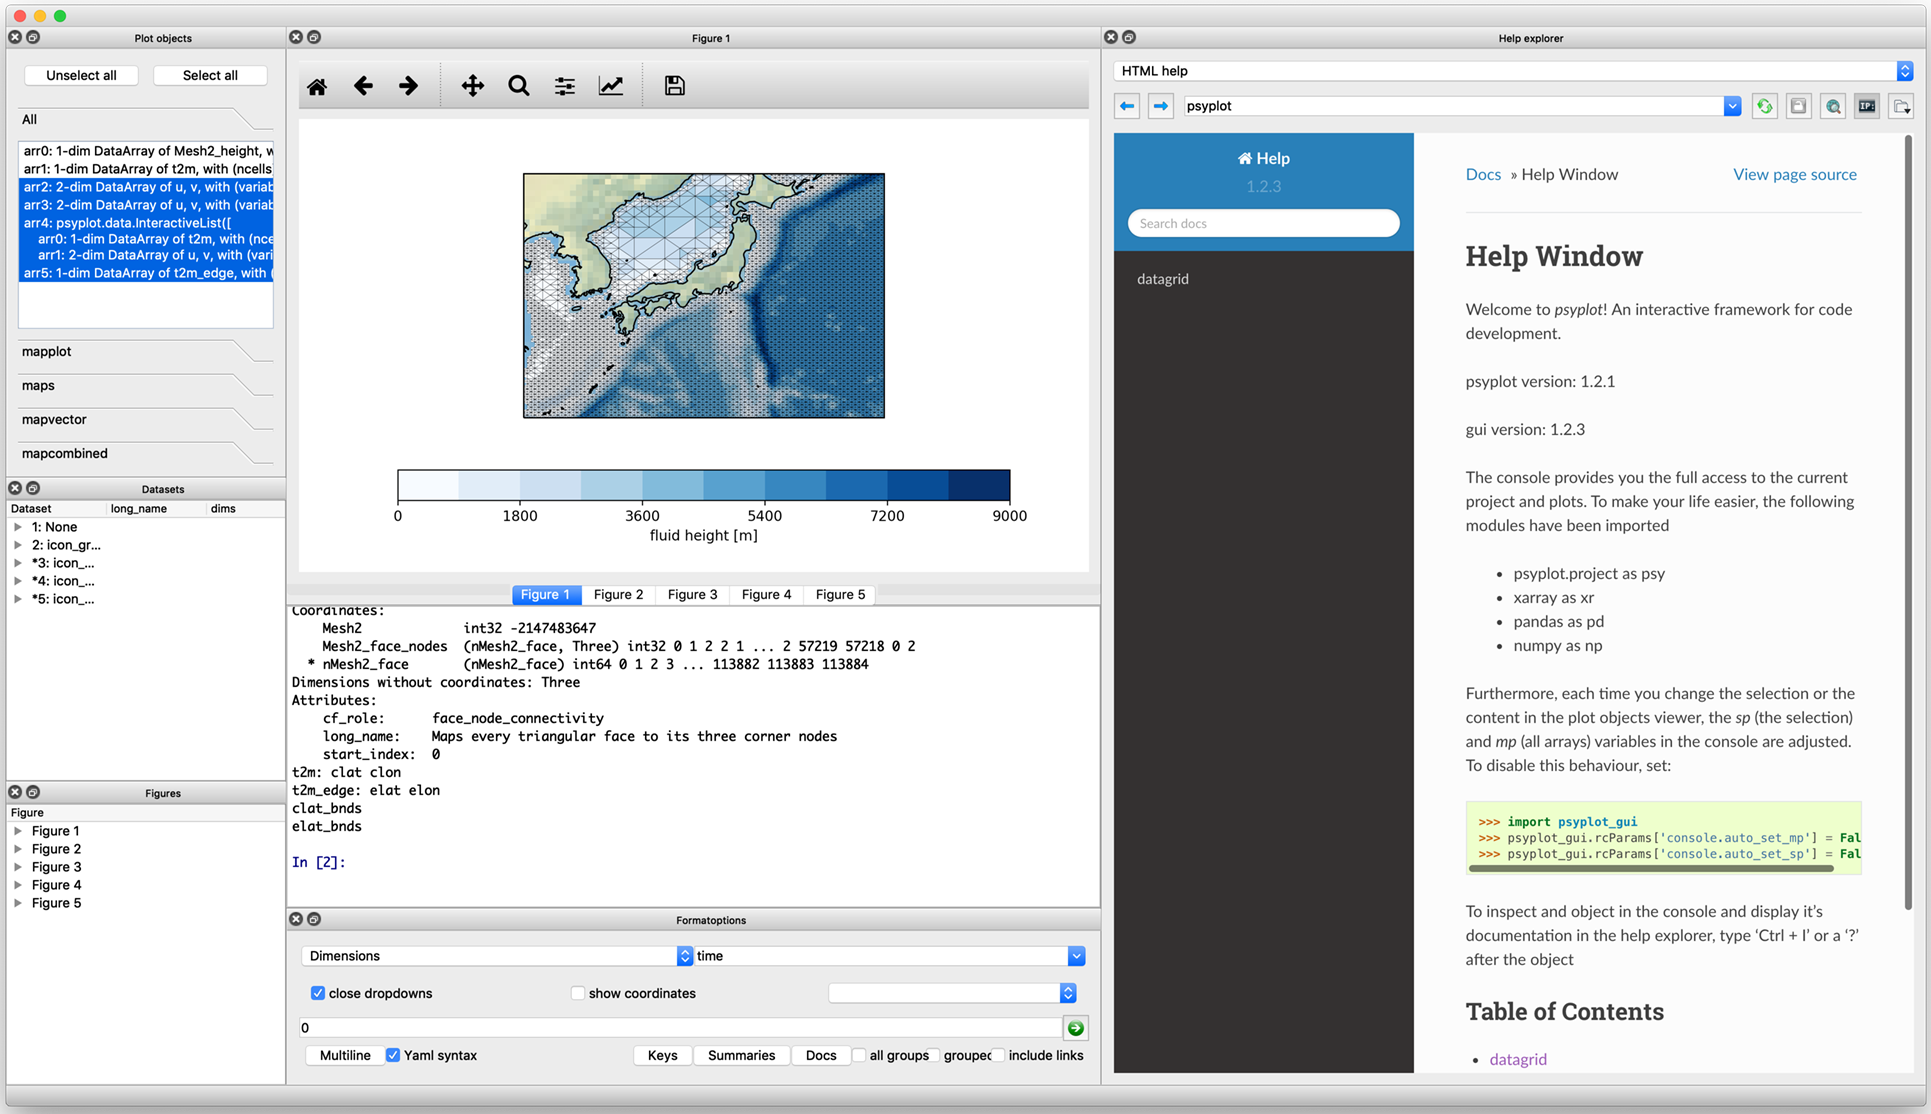
\includegraphics[width=\linewidth]{psyplot-figures/psyplot-gui.png}
	\caption[Screenshot of the psyplot GUI]{Screenshot of the psyplot \gls{gui}. The left part shows the content of the psyplot project, the upper center the plots, and the right part contains the help explorer. Below the plots, there is also the IPython console for the usage from the command line and a widget to update the formatoptions of the current project.}
	\label{fig:psyplot-gui}
\end{figure}

\begin{figure}
	\centering
	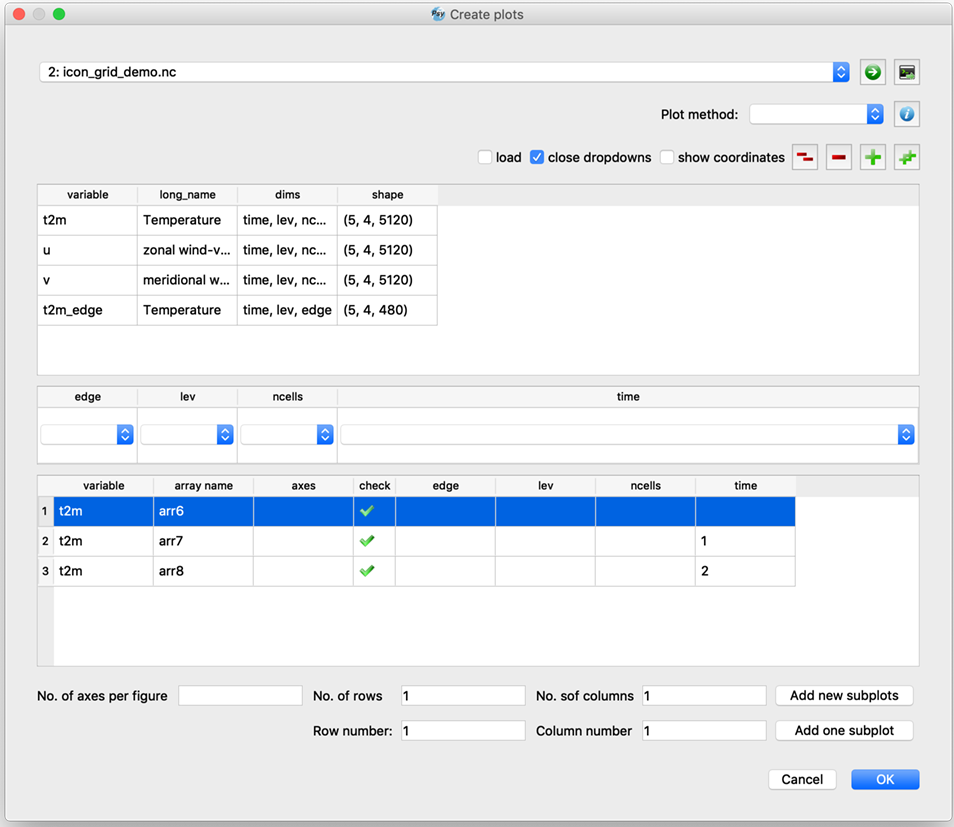
\includegraphics[width=0.7\linewidth]{psyplot-figures/plot-creator.png}
	\caption[psyplot Gui plot creation dialog]{Plot creation dialog to generate new figures from an xarray dataset.}
	\label{fig:psyplot-gui-plot-creator}
\end{figure}

Psyplots objective of providing a platform for flexible and convenient data analysis is further approached with the \textit{psyplot-gui} package. This extension to the framwork provides a \gls{gui} for simplified access to the plotting features in psyplot.

A strong focus of this interface is, again, the flexibility. psyplot-gui is based on the cross-platform PyQt5 library\footnote{PyQt5 can be accessed via \url{https://riverbankcomputing.com/software/pyqt/intro}.}, a very flexible and frequently used package for \acrlongpl{gui}. This enables other software to develop additional features for the package (see psy-strat in the previous section \ref{sec:psyplot-plugins}, for instance, or straditize in chapter \ref{chp:straditize}) and to flexibly change the layout of the application. The \gls{gui} is complemented with an interactive console to provide a fully integrated python environment for data analysis.

The next paragraphs provide an overview on the various widgets, that are also displayed in figure \ref{fig:psyplot-gui} and \ref{fig:psyplot-gui-plot-creator}. 

\subsubsection{Console}
The central aspects to guarantee flexibility of the application is an in-process IPython console, based on the qtconsole package\footnote{\url{https://github.com/jupyter/qtconsole}} that provides the possibility to communicate with the psyplot package via the command line and to load any other module or to run any other script or notebook, or even to run commands in different programming languages, such as R \citep{RCT2019} or Julia \citep{BezansonEdelmanKarpinskiEtAl2017}. The console is fully integrated both ways into the \gls{gui}. The documentation of every python object in the terminal, for instance, can be viewed in the help explorer of the GUI. And vice versa: a change of the current project through the project content widgets, also changes the corresponding python variable in the shell. 

\subsubsection{Help explorer}
As a complement to the console, the \gls{gui} contains a help explorer to provide immediate and dynamic access to the documentation of python objects in the console, rendered as an HTML webpage\footnote{The help explorer widget has been originally motivated by the \textit{Help} widget of the Scientific PYthon Development EnviRonment, Spyder (\url{https://www.spyder-ide.org/}) and uses the sphinx package \citep{Hasecke2019} to convert restructured Text into HTML.}. Furthermore, the help explorer is connected to multiple other widgets of the \gls{gui} in order to provide a dynamically generated documentation. The documentation of available formatoptions in the psyplot project, for instance, are rendered as HTML upon request, in order to make the various plot methods more accessible. The same principle works for the plot methods that are accessible in the plot creator.

\subsubsection{Plot creator}
The plot creator (figure \ref{fig:psyplot-gui-plot-creator}) is the starting point of the \gls{gui} into the psyplot framework (at least, if one does not use the console or a script to generate the plots). It loads data from the disk or the in-process console, and essentially provides a wrapper around the psyplot plotting call (see suppl. section \ref{sec:psyplot-example}). It additionally displays the documentation of the method and its associated formatoptions. This widget creates new plots, that are appended to the psyplot project and are accessible through the console and the project content widgets.

\subsubsection{Project content}
The psyplot project is the most high-level \gls{api} element in the psyplot framework (see section \ref{sec:psyplot-core}) and is displayed in the project content widgets of the \gls{gui}. All other elements, such as the formatoptions widget or the plot creator, are interfering with the project, and it is accessible as a variable in the console. The project content widget can be used to see the various items in the project, but it is also used to select the specific items for the so-called \textit{current} sub-project. The latter is dynamically set in the console through the \texttt{sp} variable and it is used by the formatoptions widget to update the plotting parameters of the selected items.

\subsubsection{Formatoptions}
As mentioned in section \ref{sec:psyplot-core}, formatoptions are the core elements in psyplot that control the figure aesthetics of the plots and/or perform data manipulations. The generic formatoptions widget provides access to these parameters, in order to update them for the selected items in the current project. The formatoption itself (i.e. the python object) can in turn generate a widget that is implemented in the formatoptions widget, to make the available options more accessible. The \textit{title} formatoption, for instance, generates a drop-down menu to select variable attributes (e.g. variable name, variable units, etc.) which is then embedded in the formatoptions widget. The modifications of the formatoptions via this widgets, updates the figures of the selected items.

\subsubsection{Figures and plots}
The plots generated by the plotting methods are displayed in dedicated widgets inside the \gls{gui} and can be dynamically adjusted using the formatoptions widget or the console. The underlying library of the current implemented psyplot plugins, matplotlib, implements multiple backends to display the data interactively, or to export them as PDF, PNG, etc. The psyplot \gls{gui} has implemented a backend on top of the PyQt5 backend of matplotlib, which embeds the figures in the \gls{gui}. psyplot can, however, work with any backend of matplotlib and does not depend on the specific implementation.

\section{Conclusions}  \label{sec:psyplot-conclusions}
psyplot \citep{Sommer2017} is a new data visualization framework that integrates rich computational and mathematical software into a flexible framework for visualization. It differs from most of the visual analytic software such that it focuses on extensibility in order to flexibly tackle the different types of analysis questions that arise in pioneering research. The design of the high-level API of the framework enables a simple and standardized usage from the command-line, python scripts or jupyter notebooks. A modular plugin framework enables a flexible development of the framework that can potentially go into many different directions. The additional enhancement with a flexible \gls{gui} makes it the only visualization framework that can be handled from the conveniently command-line, and via point-click handling. It also allows to build further desktop applications on top of the existing framework.

The plugins of psyplot currently provide visualization methods that range from simple line plots, to density plots, regression analysis and geo-referenced visualization in two dimensions. The software is currently entirely based on the visualization methods of matplotlib \citep{Hunter2007}, the most established visualization package in the scientific python community. However, the framework itself is agnostic to the underlying visualization method and can, as such, leverage a variety of existing analytical software.

\section{Outlook}  \label{sec:psyplot-outlook}

The possibilities for further development of the psyplot framework are numerous, due to \DIFdelbegin \DIFdel{it's }\DIFdelend \DIFaddbegin \DIFadd{its }\DIFaddend intrinsic generality. The core of the psyplot framework will, in the future, be extended with a standardized algorithm  for the generation of animations. Psyplot projects already have the functionality of being saved to a file and reloaded, but they will also be exportable as python scripts for a more flexible reusability and adaptability. The update process within a psyplot project (currently every item in the project is updated in parallel) also has potential for improvement by using a single-threaded scheduler approach that better reflects if one formatoption depends on the formatoptions of another plotter.

The \gls{gui} has especially high potential for further development, as it still lacks widgets to quickly and intuitively modify the visual appearance of the plots. The only possibility inside the \gls{gui} (besides the console) is to use the formatoptions widget whose main focus however is on flexibility, rather than usability and has, as such, limited possibilities for adaptation to specific use cases.

Another focus will be the development of new plot methods inside the psyplot framework. The major aspect will be on the development of 3D visualization methods of geo-referenced data, using recently published software that builds on top of the visualization toolkit VTK \citep{SullivanKaszynski2019, SullivanTrainorGuitton2019}, see \cite{Sommer2019a}. psyplot has the unique potential to generate 3D visualizations conveniently from the command line, a distinguishing feature, compared to other visualization software packages, such as ParaView or Vapor. Further potential enhancements for visualizations can involve standard interactive visual analytic tools, e.g. such that the interactive selection of features in one plot affects the visualization in another plot (so-called brushing and linking).

\clearpage

\begin{subappendices}
	\section*{Supplementary material}
	\section{Example call of a plot method}  \label{sec:psyplot-example}

	\begin{Verbatim}[commandchars=\\\{\}]
\PY{c+c1}{\PYZsh{} example call for generating a map}
\PY{k+kn}{import} \PY{n+nn}{psyplot.project} \PY{k+kn}{as} \PY{n+nn}{psy}

\PY{n}{maps} \PY{o}{=} \PY{n}{psy}\PY{o}{.}\PY{n}{plot}\PY{o}{.}\PY{n}{mapplot}\PY{p}{(}
    \PY{l+s+s1}{\PYZsq{}}\PY{l+s+s1}{psy\PYZhy{}maps\PYZhy{}demo.nc}\PY{l+s+s1}{\PYZsq{}}\PY{p}{,}  \PY{c+c1}{\PYZsh{} input file name, can also be data in memory}
    \PY{n}{name}\PY{o}{=}\PY{l+s+s1}{\PYZsq{}}\PY{l+s+s1}{t2m}\PY{l+s+s1}{\PYZsq{}}\PY{p}{,}          \PY{c+c1}{\PYZsh{} variable to plot (can also be multiples}
    \PY{c+c1}{\PYZsh{}\PYZsh{}\PYZsh{} formatoptions}
    \PY{c+c1}{\PYZsh{} colorbar label uses meta attributes of netCDF variable}
    \PY{n}{clabel}\PY{o}{=}\PY{l+s+s1}{\PYZsq{}}\PY{l+s+si}{\PYZpc{}(long\PYZus{}name)s}\PY{l+s+s1}{ [}\PY{l+s+si}{\PYZpc{}(units)s}\PY{l+s+s1}{]}\PY{l+s+s1}{\PYZsq{}}\PY{p}{,}
    \PY{c+c1}{\PYZsh{} select colormap}
    \PY{n}{cmap}\PY{o}{=}\PY{l+s+s1}{\PYZsq{}}\PY{l+s+s1}{RdBu\PYZus{}r}\PY{l+s+s1}{\PYZsq{}}\PY{p}{,}
    \PY{c+c1}{\PYZsh{} focus on a specific lonlatbox given by [lonmin, lonmax, latmin, latmax]}
    \PY{n}{lonlatbox}\PY{o}{=}\PY{p}{[}\PY{l+s+s1}{\PYZsq{}}\PY{l+s+s1}{Europe}\PY{l+s+s1}{\PYZsq{}}\PY{p}{,} \PY{l+s+s1}{\PYZsq{}}\PY{l+s+s1}{Europe}\PY{l+s+s1}{\PYZsq{}}\PY{p}{,} \PY{l+m+mi}{0}\PY{p}{,} \PY{l+s+s1}{\PYZsq{}}\PY{l+s+s1}{Europe}\PY{l+s+s1}{\PYZsq{}}\PY{p}{]}\PY{p}{)}

\PY{n}{maps}\PY{o}{.}\PY{n}{show}\PY{p}{(}\PY{p}{)}
\end{Verbatim}
  % generated with pygmentize -o example_call.text example_call.py
	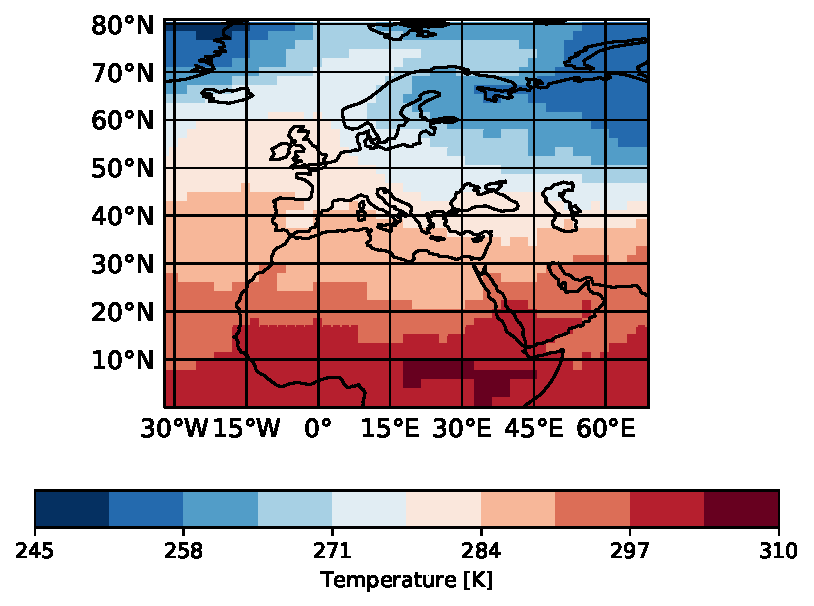
\includegraphics[width=0.45\linewidth]{psyplot-figures/example-call.pdf}

	\begin{Verbatim}[commandchars=\\\{\}]
\PY{c+c1}{\PYZsh{} Update the plot, e.g. change projection, plot global}

\PY{n}{maps}\PY{o}{.}\PY{n}{update}\PY{p}{(}\PY{n}{projection}\PY{o}{=}\PY{l+s+s1}{\PYZsq{}}\PY{l+s+s1}{robin}\PY{l+s+s1}{\PYZsq{}}\PY{p}{,} \PY{n}{lonlatbox}\PY{o}{=}\PY{n+nb+bp}{None}\PY{p}{)}
\end{Verbatim}

	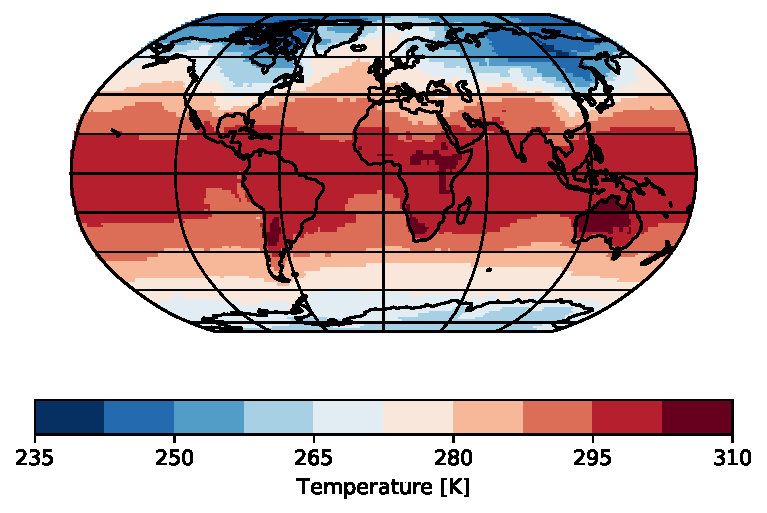
\includegraphics[width=0.6\linewidth]{psyplot-figures/example-update.pdf}

	\section{psy-simple plot methods}  \label{sec:psy-simple-plotmethods}

		\begin{tabular}[c]{l|p{0.25\linewidth}|p{0.25\linewidth}|p{0.25\linewidth}|}
			\toprule
			\textbf{Plot method} & lineplot & barplot & violinplot \\
			\hline
			\textbf{Example} & 
				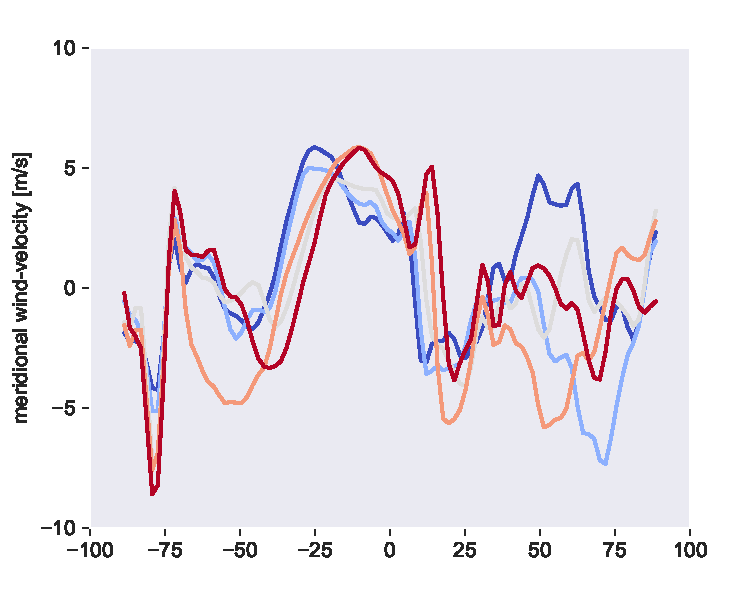
\includegraphics[width=\linewidth, page=1]{psyplot-figures/psy-simple-demo.pdf} &
				\includegraphics[width=\linewidth, page=2]{psyplot-figures/psy-simple-demo.pdf} &
				\includegraphics[width=\linewidth, page=3]{psyplot-figures/psy-simple-demo.pdf} \\
			\midrule
			\midrule
			\textbf{Plot method} & \multicolumn{3}{c}{plot2d} \\
			\hline
			\textbf{Grid type} & rectilinear & \multicolumn{2}{c}{unstructured} \\
			\hline
			\textbf{Example} & 
				\includegraphics[width=\linewidth, page=4]{psyplot-figures/psy-simple-demo.pdf} &
				\includegraphics[width=\linewidth, page=5]{psyplot-figures/psy-simple-demo.pdf} &
				\includegraphics[width=\linewidth, page=6]{psyplot-figures/psy-simple-demo.pdf} \\
			\midrule
			\midrule
			\textbf{Plot method} & \multicolumn{2}{c|}{vector} & combined \\
			\hline
			\textbf{Example} &
				\includegraphics[width=\linewidth, page=7]{psyplot-figures/psy-simple-demo.pdf} &
				\includegraphics[width=\linewidth, page=8]{psyplot-figures/psy-simple-demo.pdf} &
				\includegraphics[width=\linewidth, page=9]{psyplot-figures/psy-simple-demo.pdf} \\
			\midrule
			\midrule
			\textbf{Plot method} & \multicolumn{2}{c|}{density} & {\centering fldmean}  \\
			\hline
			\textbf{Example} & 
				\includegraphics[width=\linewidth, page=10]{psyplot-figures/psy-simple-demo.pdf} & \includegraphics[width=\linewidth, page=11]{psyplot-figures/psy-simple-demo.pdf} & \includegraphics[width=\linewidth, page=12]{psyplot-figures/psy-simple-demo.pdf} \\
			\bottomrule
		\end{tabular}


	\section{psy-maps plot methods}  \label{sec:psy-maps-plotmethods}

		\begin{tabular}{l|p{0.25\linewidth}|p{0.25\linewidth}|p{0.25\linewidth}|}
			\toprule
			\textbf{Plot method} & \multicolumn{3}{c}{mapplot} \\
			\hline
			\textbf{Grid type} & rectilinear & \multicolumn{2}{c}{unstructured} \\
			\hline
			\textbf{Example} & 
				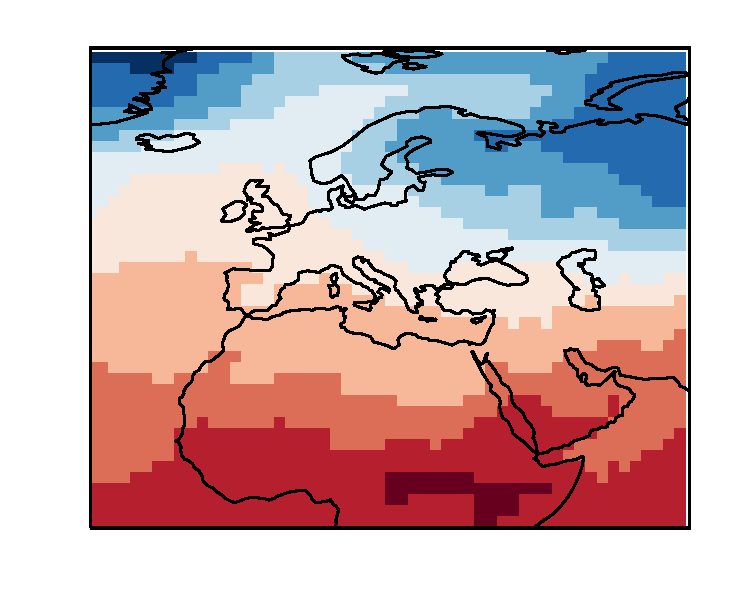
\includegraphics[width=\linewidth, page=1]{psyplot-figures/psy-maps-demo.pdf} &
				\includegraphics[width=\linewidth, page=2]{psyplot-figures/psy-maps-demo.pdf} &
				\includegraphics[width=\linewidth, page=3]{psyplot-figures/psy-maps-demo.pdf} \\
			\midrule
			\midrule
			\textbf{Plot method} & \multicolumn{2}{c|}{mapvector} & combined \\
			\hline
			\textbf{Example} & 
				\includegraphics[width=\linewidth, page=4]{psyplot-figures/psy-maps-demo.pdf} &
				\includegraphics[width=\linewidth, page=5]{psyplot-figures/psy-maps-demo.pdf} &
				\includegraphics[width=\linewidth, page=6]{psyplot-figures/psy-maps-demo.pdf} \\
			\bottomrule
		\end{tabular}

	\section{psy-reg plot methods}  \label{sec:psy-reg-plotmethods}

		\begin{tabular}{l|p{0.25\linewidth}|p{0.25\linewidth}|}
			\toprule
			\textbf{Plot method} & \multicolumn{2}{c}{linreg} \\
			\hline
			\textbf{Example} & 
				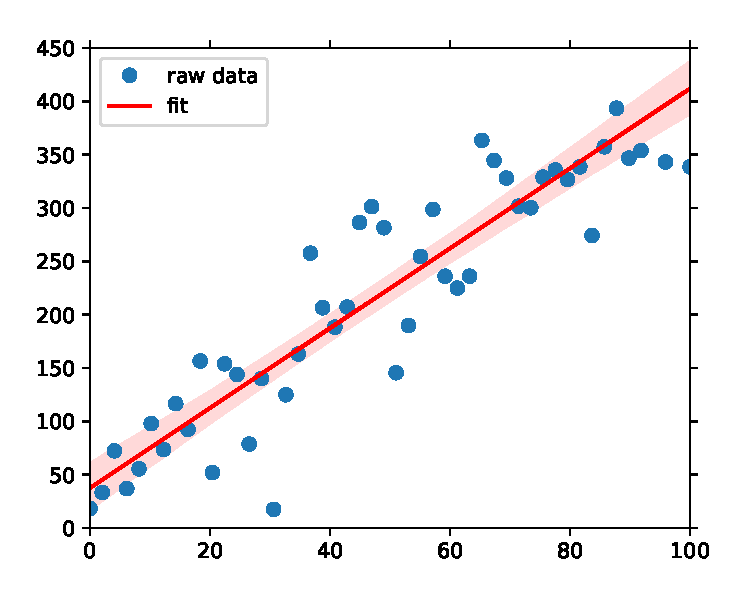
\includegraphics[width=\linewidth, page=1]{psyplot-figures/psy-reg-demo.pdf} &
				\includegraphics[width=\linewidth, page=2]{psyplot-figures/psy-reg-demo.pdf} \\
			\midrule
			\midrule
			\textbf{Plot method} & \multicolumn{2}{c|}{densityreg} \\
			\hline
			\textbf{Example} & 
				\includegraphics[width=\linewidth, page=3]{psyplot-figures/psy-reg-demo.pdf} &
				\includegraphics[width=\linewidth, page=4]{psyplot-figures/psy-reg-demo.pdf} \\
			\bottomrule
		\end{tabular}

	\section{psy-strat plot methods}  \label{sec:psy-strat-plotmethods}

		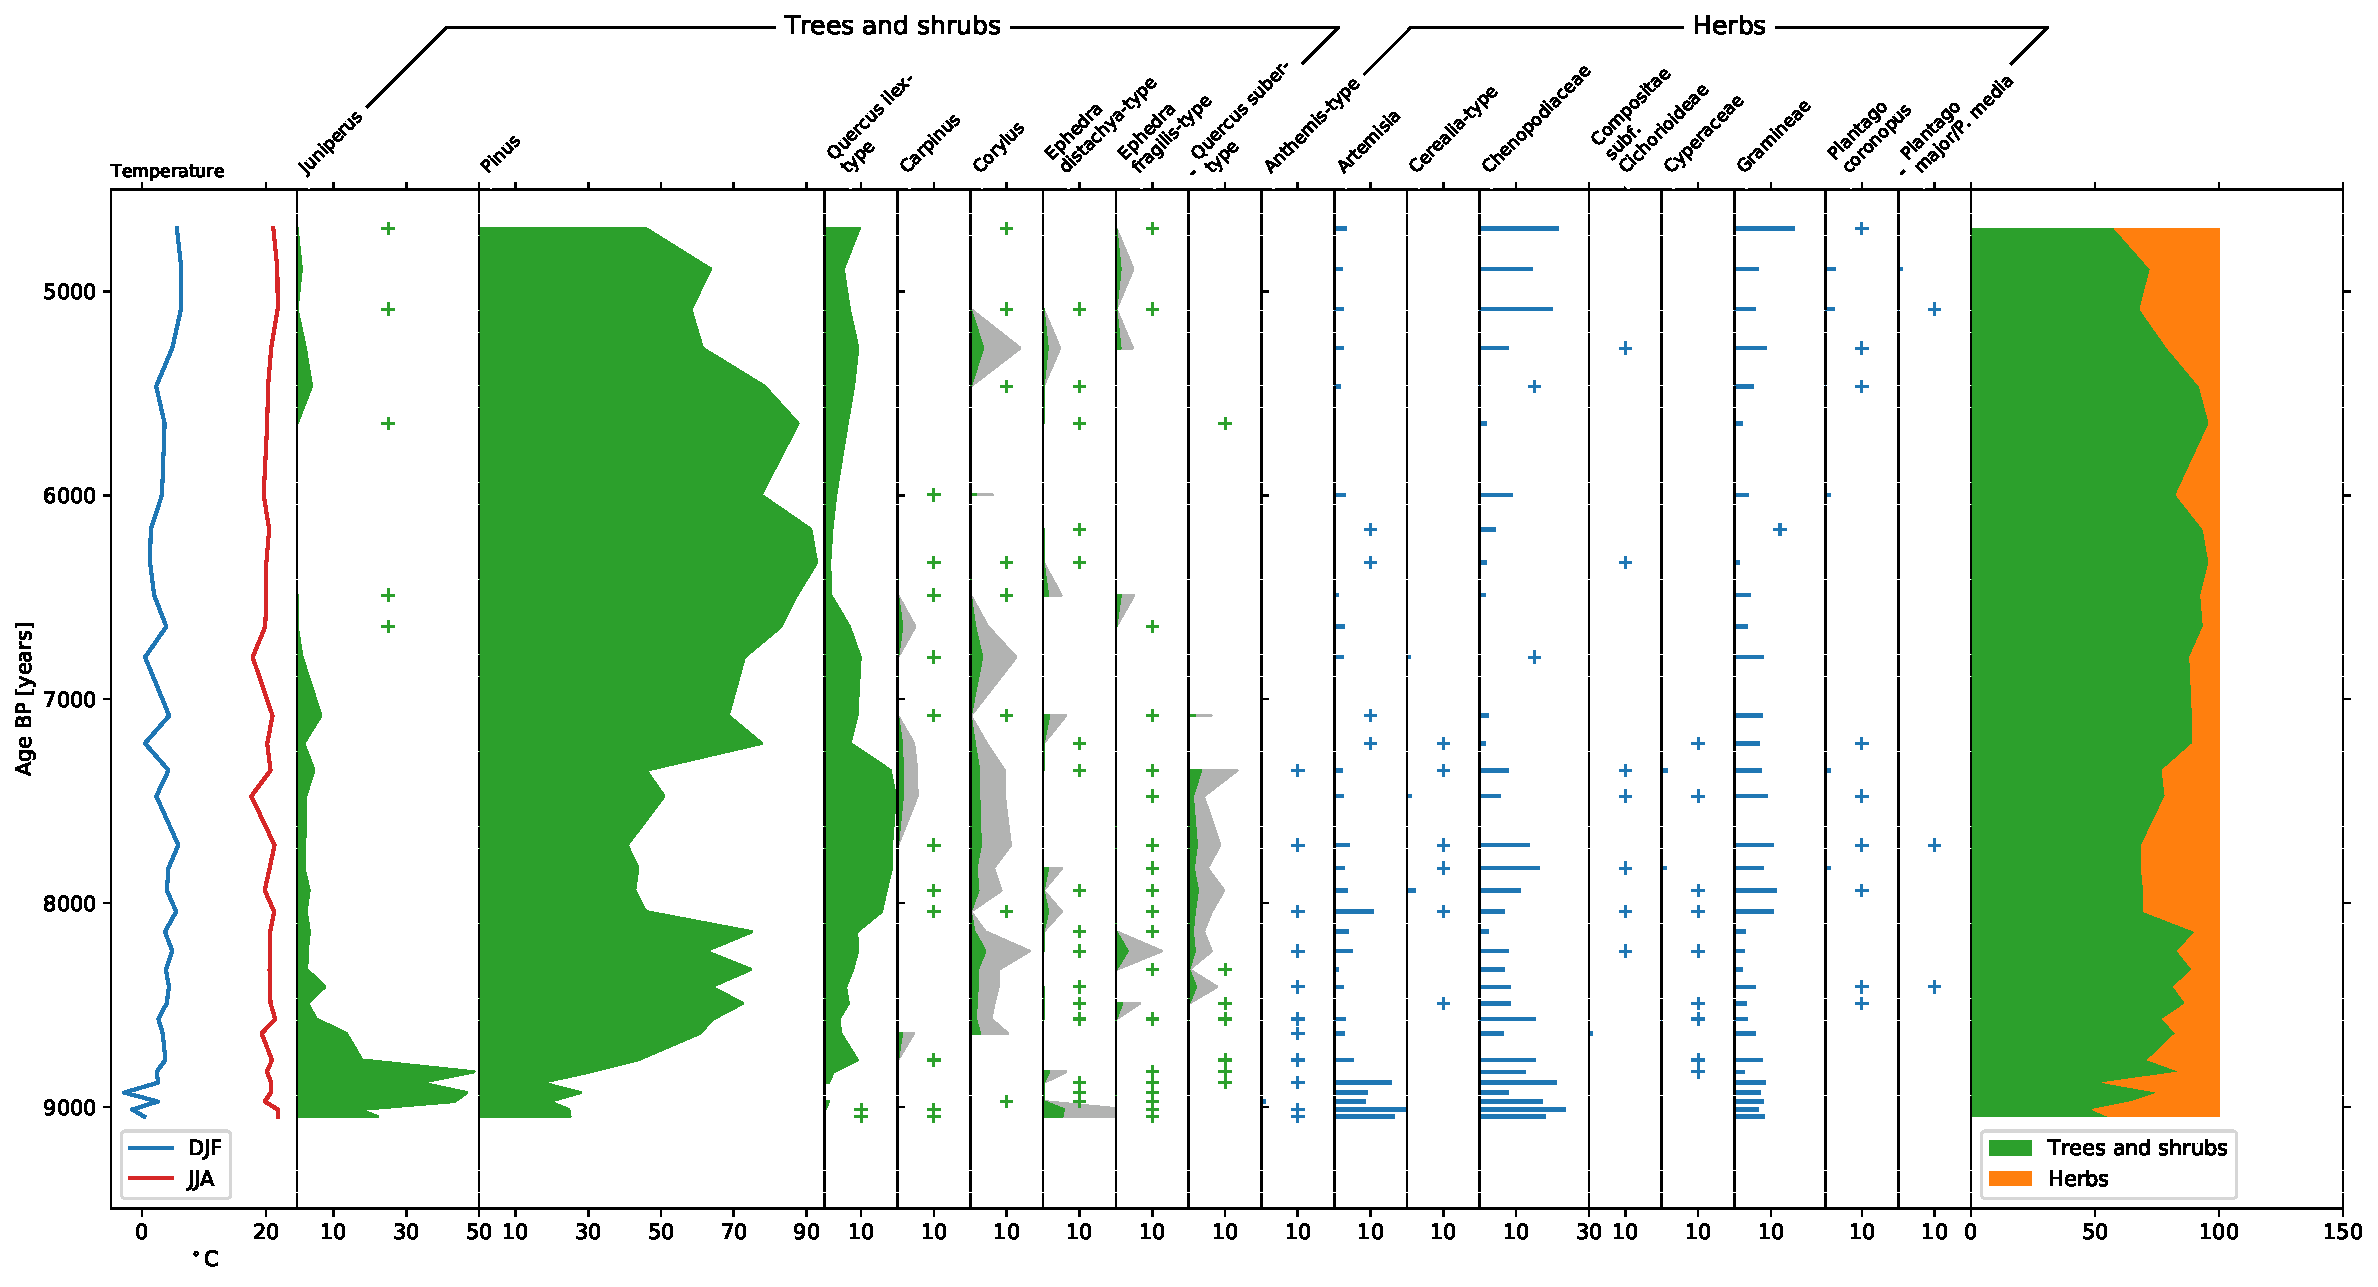
\includegraphics[width=\linewidth]{psyplot-figures/psy-strat-demo.pdf}

\end{subappendices}\

\printbibliography[heading=subbibintoc]

\end{refsection}

\part{Computational Models}  \label{part:models}

% teleconnections chapter

\Chapter{pyleogrid}{A Probabilistic Approach for Gridding Paleo Climate Data}

\label{chp:gridding}

\begin{refsection}

%----------------------------------------------------------------------------------------
%	SECTION 1
%----------------------------------------------------------------------------------------

\section{Introduction}  \label{sec:gridding-intro}

Paleo-climate reconstructions are most often undertaken on a site by site basis to provide a record of climate change at a specific place through time. The integration of data obtained from multiple sites however provides the basis for investigating spatially explicit reconstructions of climate through time. This spatio-temporal perspective can provide powerful insights into the climate system that are not easily discernible from the typical 1-dimensional approach associated with single site records. Spatially explicit data allows us to see how spatial patterns in climate variables change through time, providing a way of identifying the underlying causes of climate change. It also allows us to match the spatial scale of Earth-system models, which are based on grid-boxes that often reflect climatic changes at a very different spatial resolution than that experienced at the scale of a single site.

Here\DIFaddbegin \DIFadd{, }\DIFaddend we describe a computationally efficient methodology for integrating multiple paleo-climate records from different sites into a single spatio-temporal record that simultaneously takes into account the associated uncertainties. This method also involves projecting the data onto a uniform spatial grid and regular time-step. This approach is different from the conventional approach to gridding, often called \textit{pseudo-gridding}, in which records that fall within a grid box are simply combined in some way to represent the grid box value \citep[e.g.][]{BartleinHarrisonBrewerEtAl2010, MarsicekShumanBartleinEtAl2018, MarcottShakunClarkEtAl2013, WaelbroeckPaulKuceraEtAl2009}. Similarly, samples from the records within a grid box are also combined or binned into time-windows to create a regular time-step. \DIFdelbegin \DIFdel{Instead, our methodology leaves the data where it is in time and space and interpolates it through onto }\DIFdelend \DIFaddbegin \DIFadd{Our method instead does not aggregate the reconstruction spatially or temporally but rather interpolates the data to }\DIFaddend a user-defined 3-dimensional spatial grid and regular time-step. This approach has been used in previous studies \citep{DavisBrewerStevensonEtAl2003, MauriDavisCollinsEtAl2014, MauriDavisCollinsEtAl2015}, but here we integrate chronological and reconstruction uncertainties into the gridding process, allowing us to propagate these uncertainties through time and space onto our grid network. 

Gridding has many advantages over other simple mapping approaches, including \textit{pseudo-gridding}. It allows us to calculate more accurately area-averages and energy balances, as well as to make direct comparisons with Earth system models at a comparable grid box size and regular time-step. Gridding also allows a changing paleo-climate site/sample network through time to be stabilized, making it easier to compare one time period with another. We are also able to create a more complete record of climate in time and space, using the entire sampling network to infer climate in places and at times where we may not have a site/sample.

Our new method applies a probability approach to data integration, whereby the full uncertainty of each sample is considered in the gridding process, rather than just the sample mean used in previous \DIFdelbegin \DIFdel{methodologies }\DIFdelend \DIFaddbegin \DIFadd{methods }\DIFaddend \citep{MauriDavisCollinsEtAl2015}. From this\DIFaddbegin \DIFadd{, }\DIFaddend we can calculate the uncertainties associated with the temporal and spatial distances between our reconstruction samples/sites and the points on the grid network. We do this through an ensemble bootstrapping approach in which we repeatedly grid the data, each time using a different set of samples that are randomly generated to reflect the reconstruction and chronological uncertainties of the site network. In this study, we use pollen-data, which provides the most accessible and spatially distributed paleo-climate data available for the late-Quaternary period. 

The strength of this new \DIFdelbegin \DIFdel{methodology }\DIFdelend \DIFaddbegin \DIFadd{method }\DIFaddend is that it treats all of the paleo-climate samples and sites as a single integrated paleo-climate record from which it is possible to extract a single regionally coherent climatic reconstruction, complete with uncertainties. Pollen-based reconstructions often have high sample to sample uncertainties, and the vegetation at individual sites can be influenced by non-climatic factors such as soils, disease, fire, migration lag and human impact. Our \DIFdelbegin \DIFdel{methodology }\DIFdelend \DIFaddbegin \DIFadd{method }\DIFaddend allows us to fully utilize the large quantity of pollen-data that is available, to extract the regional background climate signal from what may be locally quite noisy data. It also has a significant advantage over other methods that integrate records using Bayesian approaches \citep[e.g.][]{HolmstroemIlvonenSeppaeEtAl2015}, in that it is much more computationally efficient, making it possible to undertake analysis at continental scales with hundreds and thousands of sites and samples. 


\section{Data}  \label{sec:gridding-data}

The ensemble based gridding method is adapted to paleo-climates. In this study, we describe the method using a large set of western Eurasian fossil pollen assemblages that have been transformed to \gls{jja} temperatures. We focus on pollen data because it is the spatially most widely available proxy during the Holocene, but it is important to mention that the reconstruction method is agnostic to the climate proxy, because it does not explicitly use the pollen assemblages but rather alters the standard climate reconstruction method under the aspect of \DIFdelbegin \DIFdel{it's }\DIFdelend \DIFaddbegin \DIFadd{its }\DIFaddend methodological uncertainties. As such, the following sections describe the fossil and modern pollen database for this use case (section \ref{sec:gridding-polnet}) and the associated uncertainties of the temperature reconstruction method (section \ref{sec:gridding-mat}) and the dating of the fossil pollen samples (section \ref{sec:gridding-ageunc}).

\subsection{Pollen database}  \label{sec:gridding-polnet}

\begin{figure}
	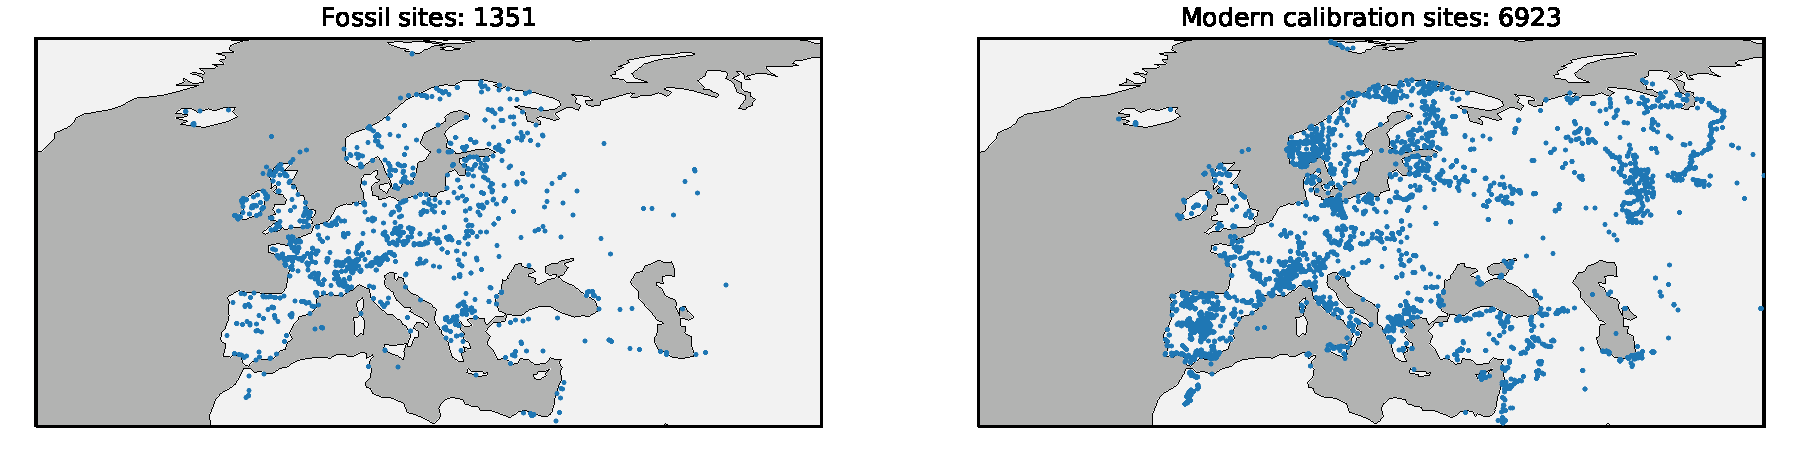
\includegraphics[width=\linewidth]{gridding-figures/sitelocs.pdf}
	\caption[Pollen Database]{Site locations of the (left) fossil and (right) modern pollen database.\todo[inline]{grey box in print}}
	\label{fig:gridding-fossil}
\end{figure}

The source data for this study is a subset of the latest development version of the POLNET database, a northern hemispheric, extra-tropical collection of pollen assemblages \citep{DavisKaplan2017, SommerDavisChevalierEtAl2019}. The purpose of this database is to generate the source for large-scale climate reconstruction during the Holocene (past 12'000 years) that can be used for model-data comparisons. The subset that we use in this study to describe and develop the gridding method contains fossil and modern pollen assemblages of western Eurasia, a region that has already been under investigation in the previous study by \cite{MauriDavisCollinsEtAl2015}. 

The fossil database contains raw pollen counts with in total about 1350 datasets that consists of 80500 fossil samples. The majority of the fossil pollen data (left part of figure \ref{fig:gridding-fossil}) comes from the \gls{epd} \citep[ca. 94\%]{FyfeBeaulieuBinneyEtAl2009} and other publicly available databases. The presented dataset extends the database used by \cite{MauriDavisCollinsEtAl2015} especially with a few sites towards the eastern part of the map.

The modern calibration dataset (6900 sames, see right map in figure \ref{fig:gridding-fossil}) is mainly based on the version 2 of the \gls{empd} \citep[ca. 87\%, see also chapter \ref{chp:empd}]{DavisZanonCollinsEtAl2013} and core tops of EPD (10\%) that were younger than 250 years cal BP.


\subsection{Sample site: Tigalmamine} \label{sec:gridding-sample-site}

\begin{figure}
	\captionsetup{width=1.2\linewidth}
	\DIFdelbeginFL %DIFDELCMD < \includegraphics[width=\linewidth]{gridding-figures/tigalmamine-analogue-map.pdf} %%%
\DIFdelendFL \DIFaddbeginFL \includegraphics[width=0.95\linewidth]{gridding-figures/tigalmamine-analogue-map.pdf} \DIFaddendFL \\
	\DIFdelbeginFL %DIFDELCMD < \includegraphics[width=\linewidth]{gridding-figures/tigalmamine-analogue-climates.pdf}
%DIFDELCMD < 	%%%
\DIFdelendFL \DIFaddbeginFL \includegraphics[width=0.95\linewidth]{gridding-figures/tigalmamine-analogue-climates.pdf}
	\DIFaddendFL \caption[Climate analogues of the Tigalmamine site]{Climate analogues of the Tigalmamine site (red cross). Every circle corresponds to one modern analogue that was one of the fifties closest analogues in at least one sample within the Tigalmamine dataset. The color-coding of each circle is based \DIFdelbeginFL \DIFdelFL{it's }\DIFdelendFL \DIFaddbeginFL \DIFaddFL{its }\DIFaddendFL corresponding country (see legend at the top). The marker size in the top plot depends on the usage of the sample as modern analogue. The larger the marker, the more samples in the Tigalmamine dataset use it as modern analogue. Tiny crosses in the map show the locations of the rest of the modern calibration data. The lower plot shows the summer temperature for the analogue (y-axis) at the age of the Tigalmamine sample (x-axis). The marker size in this plot corresponds to the chord distance between modern and fossil pollen assemblage. I.e., the larger the dot, the closer (and more important) the analogue. The dashed line shows the weighted average of all the climate analogues per sample. The age of each Tigalmamine sample is shown with the vertical lines at the bottom of the plot. Red crosses in the lower plot show the Tigalmamine core top sample that has been used as an analogue in 58 out of the 110 samples.\todo[inline]{grey box in print}}
	\label{fig:gridding-site-analogues}
\end{figure}

We chose the pollen record of Tigalmamine in Morocco (32.9N, 5.34W, 1626m) to evaluate our method. The site was first studied by \cite{LambKaars1995}, and the pollen data was downloaded from the European Pollen Database. The chronology and choice of control points used here is that from Giesecke et al \citep{GieseckeDavisBrewerEtAl2013}. The site is well dated with 11 radiocarbon dates, and spans the entire Holocene with 110 samples. The data has been used for a previously published pollen reconstruction based on the modern analogue method \citep{CheddadiLambGuiotEtAl1998}, although this study used a calibration dataset that included modern pollen samples from Morocco that have subsequently been found to have geolocation errors \citep{DavisZanonCollinsEtAl2013}. None of these problematic modern samples have been used in our analysis. 

The site (red cross in figure \ref{fig:gridding-site-analogues}) is located on the southern edge of our study region in an area with a montane Mediterranean vegetation and climate. The Mediterranean has traditionally been considered to be a particularly challenging environment for pollen-based reconstructions because of the effects of long term human impact, and the interplay of precipitation and temperature on vegetation distribution. The fossil pollen record of Tigalmamine shows a mainly forested montane Mediterranean assemblage throughout the Holocene, dominated by evergreen oak, but with an important transition between the early Holocene and late Holocene marked by a change from deciduous Oak to Cedrus (see the pollen diagram in \cite{CheddadiLambGuiotEtAl1998}). The occurrence of Cedrus represents an interesting challenge for any pollen climate transfer function, since this particular taxa is limited in its distribution (and in our calibration dataset) to Morocco and the Lebanon region, while all of the other taxa in the assemblage are widely distributed across the Mediterranean. The strong presence of evergreen Oak also makes the site interesting, because although this taxa is mainly associated with the Mediterranean region, its distribution extends all the way up the west coast of France to Brittany.

Figure \ref{fig:gridding-site-analogues} illustrates these challenges for the particular site. The climate analogues (see next section \ref{sec:gridding-mat}) span a large summer temperature regime of about 10 degrees, from 15 to 25 °C. The upper temperature range is dominated by analogue climates from Spain (orange) which in general shows the highest number analogue matches. The early Holocene (12k to 8k BP) is dominated by modern samples from Spain, with a wider and more uniform temperature regime, when compared to the later periods. During the transition in the mid-Holocene (8k to 4k BP), analogues from across the Mediterranean Sea play a more important role, in particular from Greece, Italy and Turkey. The lower temperature regime is then dominated by Moroccan samples (green) that are of particular importance during the late Holocene (4k BP to present) due to the above mentioned presence of Cedrus. 

The weighted average of the analogues (black dashed line in figure \ref{fig:gridding-site-analogues}) is in general about one to two degrees lower than the one in \cite{CheddadiLambGuiotEtAl1998} (very likely due to the above-mentioned erroneous calibration data they used). The trends are however similar: Higher temperatures in early Holocene  (the \textit{spanish analogues} dominate) with a drop around 6k BP (Moroccan climates). Our weighted average however also shows a clear increase during the past 2000 years, again driven by spanish analogues.

The climatic and geographic space that is covered by the analogues is further discussed in section \ref{sec:gridding-temperature-sampling}.

\subsection{Site-based holocene temperature estimates}  \label{sec:gridding-mat}
A standard approach for site-based climate reconstruction from fossil pollen assemblages is the \glsfirst{mat} (also called $k$-nearest neighbors). This technique estimates the climate of the fossil sample as the (weighted) climate average of the most similar modern samples (i.e. the closest modern analogues). It has the major advantage that it requires little parameterization efforts and can be applied over a large spatial area that covers many different climate regimes \citep{MauriDavisCollinsEtAl2015}. 

For this purpose, we follow the standard approach and assign \DIFdelbegin \DIFdel{a }\DIFdelend \gls{jja} temperature values \DIFdelbegin \DIFdel{to }\DIFdelend \DIFaddbegin \DIFadd{for }\DIFaddend each modern calibration sample (figure \DIFdelbegin \DIFdel{\ref{fig:gridding-modern}}\DIFdelend \DIFaddbegin \DIFadd{\ref{fig:gridding-fossil}}\DIFaddend ), taken from the corresponding grid cell in the WorldClim dataset, version 2 at 30 seconds \citep{FickHijmans2017}.

Every pollen assemblage is then transformed from raw counts to percentages, based on the total sum of terrestrial pollen counts per sample that we deem useful for the reconstruction. This excludes low samples with low counts and taxa with low occurrences. We use squared-chord distance from the R package \textit{rioja} \citep{Juggins2017} as a measure of similarity. For a given transformed fossil pollen assemblage $\left\lbrace f_{t}\right\rbrace$ and a modern pollen assemblage $\left\lbrace m_{t}\right\rbrace$, where $t=\left\lbrace1,\ldots,N\right\rbrace$ denotes one of the $N$ individual taxa in the assemblages, this distance measure is defined as

\begin{equation*}
d = \sum_{t=1,\ldots,N}\left(\sqrt{f_{t}} - \sqrt{m_{t}}\right)^2
\end{equation*}

This distance is calculated between every modern and every fossil sample in the entire database (section \ref{sec:gridding-polnet}). The standard, non-probabilistic setup would now compute the climate of the fossil sample as the mean climate of the $k$ closest analogues (e.g. $k = 6$), eventually weighted by their corresponding distance $d$. There are many variations of this technique (see for example \cite{BirksHeiriSeppaeEtAl2010}, including various measures of similarity, choices about $k$, the maximum allowed distance $d$ between modern and fossil assemblage, subsampling of the calibration dataset to avoid spatial autocorrelation \citep{GuiotVernal2011, TelfordBirks2009, TelfordBirks2005}, and by grouping pollen taxa into so-called plant-functional types (PFTs) \citep[e.g.]{DavisBrewerStevensonEtAl2003, MauriDavisCollinsEtAl2015}. They all, however, have in common that the categorical, multi-modal distribution of the climate of the modern analogues is simplified into a unimodal distribution, represented by the mean of the analogue climates. Therefore, in our ensemble approach, we do not take the mean but sample the climate of the analogues directly. This is further discussed in the methods section \ref{sec:gridding-temperature-sampling} and \ref{sec:gridding-site}.


\subsection{Age uncertainties}  \label{sec:gridding-ageunc}
In addition to the methodological uncertainties of the climate reconstruction method (previous section \ref{sec:gridding-mat}), we provide a framework to handle dating uncertainties. During the gridding step (see next section \ref{sec:gridding-gridding}), every sample is weighted by the age difference to the target reconstruction age. The previous studies by \cite{DavisBrewerStevensonEtAl2003} and \cite{MauriDavisCollinsEtAl2015} do not take this uncertainty, that can be as high as multiple centuries, into account although they influence the gridded temperature reconstruction.

The reason is a systematic problem of pollen samples that we overcome here with the recent developments in the pollen community. In palynology, each sample in a sediment core is is dated using a so-called age-depth model, a function that maps each depth of the sediment core to an age. This function is based on a few chronological control points where the age has been determined instrumentally (for lake sediments in the Northern Hemisphere, these are commonly radiocarbon ($^{14}$C dates) and interpolates/extrapolates to the depths of the sample locations. Various methodologies exist to define these age-depth models, ranging from simple linear interpolation methods \citep{Bennett1994} to the more recently developed bayesian techniques of the Bchron \citep{HaslettParnell2008} and BACON \citep{BlaauwChristen2011} models.

The early approaches have been proven to provide unreliable uncertainty estimates \citep{TelfordHeegaardBirks2004} and there has been no standardized way to report the uncertainties, if they are reported at all. For this reason we (and previous studies) cannot rely on the age uncertainties reported in the pollen database. An alternative approach is to recalculate the chronology for every dataset in the database \citep[see][for instance]{Goring2019}, but this also requires parameterization for reliable uncertainties and goes beyond the scope of this study.

Instead, we follow an approach that is based on two aspects: age uncertainties are higher for older samples, and samples that are farther away from the radiocarbon dates (i.e. chronological control points). Additionally, samples behave differently if the sample is surrounded by two chronological points (i.e. the sampe age is interpolated) or not (sample age is extrapolated). To quantify these relationship, we perform a study based on all datasets (ca. 30'000 samples) from the Neotoma paleoecology database \citep{WilliamsGrimmBloisEtAl2018} that have age-depth models estimated with BACON, a model that has been proven to provide more reliable age uncertainty estimates \citep{TrachselTelford2016}. For the sake of implementation (the age sampling in section \ref{sec:gridding-age-sampling} assumes a normal distribution), we apply several assumptions and proximations to the Neotoma samples, in particular:
%
\begin{enumerate}
	\item We assume that every dataset with a BACON chronology in Neotoma keeps the defaults and reports the limits of the 95\% confidence interval (CI)
	\item We keep only the maximal distance of the CI limits from the reported age (i.e. we assume a symmetric distribution)
	\item We assume that the distribution is normal (i.e. the 95\% CI corresponds to the $2\sigma$ interval, where $\sigma^2$ denotes the scale parameter) and a division in half of the maximal distance (see previous assumption) gives the standard deviation $\sigma$ (which is what we call the age uncertainty)
\end{enumerate}
%
The resulting data is illustrated in figure \ref{fig:gridding-univariate-age-unc}. The grayscale density plots in the background shows the high dispersal of the data and the number of samples decreases strongly with higher distance to the control point or older samples (red lines). Nonetheless, the mean of the data (blue lines) reveals the increasing nature of both relationships, as mentioned before.

Figure \ref{fig:gridding-univariate-age-unc} also shows two models that have been fitted to the data. The first one is a standard simple univariate linear model $y = a + b\cdot x$ (orange line). This model simulates the increasing trend of both variables although it does not capture the non-linear relationship between age and age-uncertainty. A reason for this non-linearity arises from the time-dependency of the radiocarbon calibration curve and \DIFdelbegin \DIFdel{it's }\DIFdelend \DIFaddbegin \DIFadd{its }\DIFaddend associated errors. This non-linear behavior gives the motivation to use a constrained linear \gls{gam}, a smooth semi-parametric model of the form
%
\begin{equation*}
	\mathbb{E}[y|X] = \beta_0+f_1(X_1)
\end{equation*}
%
in the univariate case, or
%
\begin{equation*}
\mathbb{E}[y|X] = \beta_0+f_1(X_1)+f_2(X_2)
\end{equation*}
%
in the bivariate case. The feature functions $f_1$ and $f_2$ are based on penalized B splines with a constraint for monotonic increasing, the expected value $\mathbb{E}[y|X]$ is based on a normal distribution. The \gls{gam} model has been fitted with the \textit{pyGAM} software package \citep{ServenBrummittAbedi2018}. This model enables to better simulate the non-linear features as can be seen with the green lines in figure \ref{fig:gridding-univariate-age-unc}.

These results approve the initial hypotheses and justify the choice of a bivariate \gls{gam} for predicting age uncertainties based on the distance to the chronological control point, and the age of the sample. The two models, together with a bivariate simple linear regression model, and again for interpolated and extrapolated samples, are shown in the central column of figure \ref{fig:gridding-bivariate-age-unc}. Both model classes (simple linear and \gls{gam}) are able to reproduce the general shape of the observed data, although the \gls{gam} better resolves the non-linear relationship between the three variables.

The final uncertainties, predicted for the data set presented in the previous section \ref{sec:gridding-polnet}, are shown in the supplementary figure \ref{fig:gridding-age-uncertainties}.

\begin{figure}
	\captionsetup{width=\linewidth}
	\includegraphics[width=\linewidth]{gridding-figures/univariate-models.pdf}
	\caption[Univariate age uncertainty models]{Univariate regression plots of (first and third) distance to chronological points, and (second and fourth) age to the one sigma dating uncertainty of the sample. The upper two plots contain only interpolated samples (i.e. samples that lie between two chronological control points), the lower extrapolated samples. Blue lines show the mean age uncertainty for the given distance (age). Orange and green lines show the linear and \gls{gam} fits of distance (age) to age uncertainty, and red lines show the number of samples for a given distance (age). The grayscale plot in the background shows a two-dimensional histogram (density plot) to illustrate the underlying data of the fits. For the purpose of a better visualization, each vertical bin of this histogram has been normalized to one. Means, counts and histogram are all based on 100 year bins in distance (age). The fits are estimated based on the unbinned data, the source data are all Neotoma datasets with BACON-based age-depth models. Note the logarithmic scale of the right count axis on the first and third plot.}
	\label{fig:gridding-univariate-age-unc}
\end{figure}

\begin{figure}
	\includegraphics[width=\linewidth]{gridding-figures/bivariate-models.pdf}
	\caption[Univariate age uncertainty models]{Bivariate models of age uncertainty. Shown are the mean $1\sigma$ age uncertainties of ca. 30'000 samples from the Neotoma database sites with BACON-based age-depth models. Each sample has an age uncertainty that depends on the age of the sample (x-axis) and the distance to the closest chronological control point (y-axis). For the purpose of visualization, we grouped the samples into categories of 100 years in x- (age) and 100 years in y- (control point distance) direction, and calculated the average age uncertainty of the groups. These averages are shown with the color coding in the plots, and the gray area represents the space without any observation. The top row shows interpolated samples (i.e. samples that lie between two chronological control points), the bottom row extrapolated samples. Plots in the left column show the observed mean age uncertainties, central and right columns show the means of the predicted age uncertainties from the bivariate linear \glspl{gam} and bivariate linear regression models respectively. }
	\label{fig:gridding-bivariate-age-unc}
\end{figure}

\section{Method}  \label{sec:gridding-method}
With the intrinsic methodological uncertainties of climate and dating in mind, we present a new ensemble-based approach on gridding the reconstructions from the individual sites. Each ensemble member is generated with randomized sample ages and climate, derived from the corresponding uncertainty measures (see previous sections \ref{sec:gridding-mat} and \ref{sec:gridding-ageunc}), with additional constraints arising from the integrity of the individual dataset (sediment core). We explain these in more details in sections \ref{sec:gridding-age-sampling} and \ref{sec:gridding-temperature-sampling}. The final gridding step for each ensemble member is based on a modified setup of \cite{MauriDavisCollinsEtAl2015}, but can also be extended with other interpolation algorithms, as described in section \ref{sec:gridding-gridding}). We implemented the method as the python package \textit{pyleogrid} that efficiently scales to large datasets and ensemble sizes, and shortly describe it in section \ref{sec:gridding-package}.

\subsection{Constrained age sampling}  \label{sec:gridding-age-sampling}

\begin{figure}
	\includegraphics[width=\linewidth]{gridding-figures/age-sampling-methods-realized.pdf}
	\caption[Scaled histograms of age sampling methods]{Histograms of age sampling methods for the site in section \ref{sec:gridding-sample-site} with an ensemble size of 10'000. Every sampled age has been centered at the reported age of the corresponding sample and scaled by its age uncertainty. The black line shows the unconstrained distribution (a standard normal with a standard deviation of 1), the other histograms show the realized distributions for each of the age sampling methods (section \ref{sec:gridding-age-sampling}). Note that \textit{random sort} and \textit{Gibbs} histograms highly overlap.}
	\label{fig:gridding-age-sampling-methods}
\end{figure}

Every dataset has an intrinsic monotonicity constraint that the sample deeper down the core has an older age. An inversion of this constraint is very rare and is usually visible in the stratigraphy of the core, such that affected samples are ruled-out before. As such, a classic unconstrained sampling of ages\footnote{\label{foot:unconstrained-note}We call it the unconstrained distribution for convenience, but keeping in mind that every sampled age has to be older than -70 yr cal BP.} using a normal distribution centered at reported sample age and a scale corresponding to the estimated age uncertainty (section \ref{sec:gridding-ageunc}) violates this constraint. Samples are inverted in such a case when their uncertainty intervals overlap and as such the individual ensemble member would not maintain the integrity of the individual core. We illustrate an example for such a core in section \ref{sec:gridding-site}.

\textit{pyleogrid} therefore implements different variants of this constraint with the Gibbs sampling being the one that is finally used.

\subsubsection{The intuitive approach}
The most intuitive approach is to randomly draw a sample age and \DIFdelbegin \DIFdel{constraint }\DIFdelend \DIFaddbegin \DIFadd{constrain }\DIFaddend the age of the neighboring sample with it. This can be done in a \textit{forward} manner, such that every older sample has to be older than the previous younger sample, or in a backward manner, i.e. the younger sample has to be younger than the neighboring older sample. We will show in the paragraphs below that this method is biased, nevertheless we mention it here because of the intuitivity of the approach and because the reason for the failure is non-trivial.

As such, we demonstrate three different algorithms:

\begin{description}
	\item[forward] Starting with an unconstrained age distribution for the youngest sample in the core, every consecutive sample has to be older than the previous (i.e. the method works forward in age, but backward in time
	\item[backward] Starting with an unconstrained age distribution for the oldest sample in the core, every consecutive sample has to be younger than the previous (i.e. the method works backward in age, but forward in time)
	\item[random start] Starting with an unconstrained age distribution of a random sample in the core, we apply the \textit{backward} algorithm for younger and \textit{forward} algorithm for younger samples.
\end{description}

As such, \textit{forward} and \textit{backward} algorithms always start with an unconstrained age distribution of the youngest (oldest) sample for every ensemble member. Within the \textit{random start} algorithm, every sample gets the chance to start with an unconstrained age distribution, because the starting point is random for every ensemble member. The constrained age distributions for the consecutive samples are implemented as truncated normal distributions.

The resulting age distributions from the three algorithms are shown in figure \ref{fig:gridding-age-sampling-methods}, together with another method, that is described later in this section. The figure shows the sampled age distributions by the various above-mentioned sampling methods for the site described in section \ref{sec:gridding-sample-site}. To make these age distributions comparable, we transformed them to a standard normal distribution (visualized as the unconstrained distribution in figure \ref{fig:gridding-age-sampling-methods}) prior to visualization, by subtracting the reported age and dividing by the estimated age uncertainty of the corresponding sample. It is obvious from this figure that all of the above-mentioned algorithms produce an artificial bias to the age distribution. The \textit{forward} approach pushes the samples to the upper tail of the distribution, the \textit{backward} approach pushes everything to the lower tail. The \textit{random start} method produces a bimodal distribution with peaks at the upper and lower tail.

This is also shown with three exemplary samples from the site in the supplementary figure \ref{fig:gridding-age-example-distributions}. The forward method works well for the young sample but pushes all older samples to the upper tail of their distribution, The backward method does the opposite and the random sort method creates a bimodal distribution for the sample in the center of the core, and backward behaves like the forward (backward) algorithm at the older (younger) part of the core.

We explain this initially unexpected results with the overlapping age uncertainties in the core. The site that we describe here has 110 samples. As such, the probability that one sample draws a random age at the lower or upper tail of the distribution is very high. Now, most of the dating uncertainty intervals overlap and this forces all the consecutive samples to the tail of their age distributions. Another problem, that is not shown here, arises from the differing sizes of the age uncertainties which highly depends on the distance to the chronological control point (see section \ref{sec:gridding-ageunc}). This can also lead to unsatisfiable requirements, if one sample is close to a control point (and as such has a lower age uncertainty) and the previous sample has been pushed far outside of the 95\% confidence interval.


\subsubsection{The random sorting approach}

These strong biases of the intuitive approach led to another method, that we also show in red in figure \ref{fig:gridding-age-sampling-methods} and supplementary figure \ref{fig:gridding-age-example-distributions}, the \textit{random sort} method. This method consists of two steps: in the first step we draw random age for each sample based on its unconstrained distribution\textsuperscript{\ref{foot:unconstrained-note}}. In the second step, we order these random ages while maintaining the order of samples in each dataset. As such, we assign an age to each sample that is not necessarily drawn from its own distribution, but rather from the one of a neighboring sample. When samples overlap, this then truncates the tails of realized distribution and effectively decreases the reported age uncertainty, as can be seen in the figures \ref{fig:gridding-age-sampling-methods}, \ref{fig:gridding-age-example-distributions}. This approach is mathematically difficult to justify because it violates the common methodology that each sample has a unique confidence interval that it needs to explore. Therefore the method might introduce some hidden biases in the sampled distributions that are difficult to quantify. Nevertheless, the algorithm is very fast and much closer to the desired joint distribution, than the previous \textit{intuitive} approach. But in order to avoid any biases and to guarantee a mathematically correct result, we chose to implement a Gibbs sampling algorithm to sample from the desired constrained distribution.


\subsubsection{The Gibbs sampling approach}

\begin{figure}
	\includegraphics[width=\linewidth]{gridding-figures/full-realized-age-distribution.pdf}
	\caption[Realized age distribution for the entire dataset]{Realized age distribution for the entire dataset (section \ref{sec:gridding-polnet}) with the \textit{random} method (section \ref{sec:gridding-age-sampling}). The individual sample distributions have been centered and scaled as in figure \ref{fig:gridding-age-sampling-methods}.}
	\label{fig:gridding-full-age-distribution}
\end{figure}

\begin{algorithm}[h]
\renewcommand{\algorithmicensure}{\textbf{Output:}}
\caption[Accept/Reject algorithm]{Accept/Reject algorithm. $\mathcal{N}(\mu, \sigma)$ denotes the normal distribution with location parameter $\mu$ and shape parameter $\sigma$.}
\label{a:gridding-mcmc}
\begin{algorithmic}[1]
	\STATE Set $i = 0$
	\STATE Set $\boldsymbol{\mu}$ as vector of the reported ages in $dataset$
	\STATE Set $\boldsymbol{\sigma}$ as vector of estimated age uncertainties		
	\STATE Set $\mathbf{a}$ (the target age vector) to be of length $\boldsymbol{\mu}$
	\WHILE{$i < 1$ \OR \NOT $is\_monotonic(\mathbf{a})$}
	\STATE $\mathbf{a} = \mathcal{N}(\boldsymbol{\mu}, \boldsymbol{\sigma}^2)$
	\STATE Set $i = i + 1$
	\ENDWHILE
\end{algorithmic}
\end{algorithm}

The biases of the above-mentioned algorithms led to the development of a \gls{mcmc} sampling algorithm. An accept/reject algorithm\DIFaddbegin \DIFadd{, }\DIFaddend which draws a set of random ages for all unconstrained sample distributions in a core at once and accepts the draw if the monotonicity condition\DIFaddbegin \DIFadd{, }\DIFaddend is satisfied and rejects the sample if the monotonicity condition was initially explored. For one realization of the ages $\mathbf{a}$ in a given dataset, this is described with the pseudo-code in algorithm \ref{a:gridding-mcmc}. This standard approach however did not find a monotonic solution within ten million iterations for a high-resolution site such as it has been used in the previous section. 

Therefore we decided to implement a Gibbs sampler, an algorithm that is commonly used in Bayesian inference to obtain a sequence of samples from conditional probability distributions, which generate samples from a multivariate joint distribution when this distribution is unknown and/or cannot be sampled directly. In our case, this distribution if the distribution of all sample ages in one dataset, where each sample age is conditioned by \DIFdelbegin \DIFdel{it's }\DIFdelend \DIFaddbegin \DIFadd{its }\DIFaddend younger and older neighbor. Let $\boldsymbol{\mu} = \left(\mu_1, \mu_2, \ldots \mu_N \right)$ be the reported ages of the $N$ pollen samples in one individual dataset with estimated age uncertainties $\boldsymbol{\sigma} = \left(\sigma_1, \sigma_2, \ldots \sigma_N \right)$. The reported ages fulfill the monotonicity constrain, i.e. $\mu_j \leq \mu_k$ for all $j, k$ with $1 \leq j \leq k \leq N$. The objective of our sampling approach is to generate $M$ random realizations of $\boldsymbol{\mu}$, denoted by $\mathbf{X}^{(m)} = \left(X^{(m)}_1, X^{(m)}_2, \ldots X^{(m)}_N \right)$ with $m=1,\ldots,M$, that all fulfill the monotonicity constrain. In other words, the realizations $\mathbf{X}^{(m)}$ are constrained to fulfill

\begin{equation}
	X^{(m)}_j \leq X^{(m)}_k, \text{ for all } j, k \text{ with } 1 \leq j \leq k \leq N \text{ and } 1\leq m \leq M.
\end{equation}

We set the intial value to the reported ages ($\mathbf{X}^{(1)} = \boldsymbol{\mu}$) where we know that the constrain is fullfilled. For the following realizations $\mathbf{X}^{(m+1)}$ with $1 < m \leq M$ we sample each component $X_j^{(m)}$ with $1 \leq j \leq N$ conditioned by its previous sample $X_{j-1}^{(m)}$ and, most importantly, conditioned by the next sample, but from the previous realization, i.e. $X_{j+1}^{(m-1)}$. As such, we define the sampled age of $X_j^{(m)}$ with

\begin{equation}
	X^{m}_j = \mathcal{N}(X_{j-1}^{(m)}; X_{j+1}^{(m-1)}; \mu_j, \sigma_j^2)
\end{equation}

where $\mathcal{N}(a; b; \cdot, \cdot)$ denotes a random variate of the truncated normal distribution with lower limit $a$ and upper limit $b$. Although this algorithm always starts with the youngest sample in the dataset for every realization, such as the \textit{forward} method, it does not push every sample to the lower tail of the distribution because every sampled age is conditioned by the age of the next pollen sample from the previous realization. It is mathematically proven that the combined realizations $\left\lbrace\mathbf{X}^{(1)}, \mathbf{X}^{(2)}, \ldots \mathbf{X}^{(M)}\right\rbrace$ of this algorithm approximates the joint distribution of the sample ages in the dataset under the given constraint, and that each marginal distribution of a the age of a particular pollen sample $1 \leq j \leq N$ is approximated by $\left\lbrace X_j^{(1)}, X_j^{(2)}, \ldots, X_j^{(M)} \right\rbrace$.

As it is common for a \gls{mcmc} algorithm, each realization is correlated with nearby realizations. The first samples are particularly correlated with the initial value $\boldsymbol{\mu}$ and it is therefore common practice to discard the first 1000 realizations, the so-called \textit{burn-in} period. 

To avoid an autocorrelation between the successive realizations, we \textit{thin} our set of sampled ages and keep only every tenth realization until we have the desired amount of $M$ realizations. The value of 10 has been shown to be sufficient using an autocorrelation analysis of the different samples in the Tigalmamine record.

As can be seen in figure \ref{fig:gridding-age-sampling-methods} and \ref{fig:gridding-age-example-distributions}, the outcomes are very close to the above mentioned \textit{random sort} approach. However, a look into the realized distribution of the last sample in figure \ref{fig:gridding-age-example-distributions} reveals a negative bias of the distribution sampled with the \textit{random sort} approach.

The realized (and standardized) distribution of the entire database presented in section \ref{sec:gridding-polnet} is finally shown in figure \ref{fig:gridding-full-age-distribution}. The comparison with the unconstrained distribution in this figure highlights the need for a constrained sampling because the latter significantly reduces the width of the distribution.

\subsection{Temperature sampling}  \label{sec:gridding-temperature-sampling}

\begin{figure}[h]
	\includegraphics[width=\linewidth]{gridding-figures/temp-sampling-methods-realized.pdf}
	\caption[Scaled histograms of temperature sampling methods]{Histograms of temperature sampling methods for the site in section \ref{sec:gridding-sample-site} with an ensemble size of 10'000 for a climatic constraint of (left) 2 °C, and (right) 5 °C. As in figure \ref{fig:gridding-age-sampling-methods}, every sampled temperature has been centered at the weighted average of the corresponding modern analogues and scaled by the corresponding weighted standard deviation. The black line shows the unconstrained distribution (a standard normal with a standard deviation of 1), the other histograms show the realized distributions for \textit{random start} and \textit{Gibbs} temperature sampling method (section \ref{sec:gridding-age-sampling}).}
	\label{fig:gridding-temp-sampling-methods}
\end{figure}

\begin{figure}[!t]
	\includegraphics[width=\linewidth]{gridding-figures/tigal-sample-climate-violins.pdf}
	\caption[Realized temperature distributions for a few samples]{Violin plots for sampled temperature distributions of some samples in the Tigalmamine record with a climatic threshold of (top) 2 and (bottom) 5 °C. Blue (left) distributions are realized with the \textit{random start} method, ocher (right) areas with Gibbs sampling. The crosses to the left of each violin shows the locations of the climate analogues. Each cross is color coded by \DIFdelbeginFL \DIFdelFL{it's }\DIFdelendFL \DIFaddbeginFL \DIFaddFL{its }\DIFaddendFL chord distance relative to the chord distance of the closest analogue (i.e. the closest analogue has always a weight of 1).}
	\label{fig:gridding-temp-sampling-violins}
\end{figure}

As already mentioned in \ref{sec:gridding-mat}, our sampling approach does not use the temperature and uncertainty reported for every single variable. Instead, it samples the underlying distribution. As such, our method can be adapted to multiple site-specific reconstruction methods, such as weighted averaging (WA), weighted-averaging partial-least squares (WAPLS) \citep{BirksBraakLineEtAl1990, BraakJuggins1993} or other approaches \citep[e.g.][]{BirksHeiriSeppaeEtAl2010, BrewerGuiotBarboni2007, Juggins2013}. In this study, we use a \gls{mat} approach (see section \ref{sec:gridding-mat}) and sample the discrete set of climate analogues for each sample. The probability to select an analogue (i.e. \DIFdelbegin \DIFdel{it's }\DIFdelend \DIFaddbegin \DIFadd{its }\DIFaddend weight) is thereby determined by the chord distance between the fossil and modern pollen assemblages. The closer the assemblages (relative to the other potential analogues), the higher the weight.

This methodology is substantially different from the standard approach, such that \DIFdelbegin \DIFdel{is }\DIFdelend \DIFaddbegin \DIFadd{it }\DIFaddend takes the multimodality of the analogues into account, whereas the standard \DIFdelbegin \DIFdel{appraoch }\DIFdelend \DIFaddbegin \DIFadd{approach }\DIFaddend (weighted average of the $k$ closest analogues) estimates a unimodal distribution. It additionally better represents the discrete nature of the analogue approach whereas the standard method intrinsically assumes a continuity in the distribution. In fact, only a small part of the available climate space is actually represented by the modern analogues. The 5'500 modern analogues for Tigalmamine, for instance (110 samples with 50 analogues each), are represented by only 240 distinct modern pollen samples with only 131 distinct \gls{jja} temperatures and they eventually span a large climate space (see figure \ref{fig:gridding-site-analogues}).

The latter gives the motivation for a climatic constraint that ensures the integrity of the individual dataset. It is, for instance, impossible that two samples from the same dataset but 200 years apart experience a temperature difference of five degrees or more between each other. This is, however, a possible combination, considering the underlying set of analogues (see figure \ref{fig:gridding-site-analogues} for instance). We therefore perform a constrained sampling, as in section \ref{sec:gridding-age-sampling}, and implement a fixed temperature threshold $T$. Every sampled analogue in each dataset (i.e. every choice of the discrete distribution for each pollen sample) is constraint to not differ by more than $T$ \DIFdelbegin \DIFdel{degrees celsius }\DIFdelend \DIFaddbegin \DIFadd{degree Celsius }\DIFaddend from its temporally neighboring samples. The exact choice of $T$ is a critical assumption and has a major impact on the realized temperature distribution for each sample. We decided for a very conservative estimate of five \DIFdelbegin \DIFdel{degrees}\DIFdelend \DIFaddbegin \DIFadd{degree Celsius}\DIFaddend , which is only applied if the samples do not differ by more than 1000 years. These choices are further discussed in section \ref{sec:gridding-results}.

In the remainder of this section, we focus on the implementation of this conditional sampling, because of its substantial impact on the realized distribution, as already shown for the sampled ages in section \ref{sec:gridding-age-sampling}. We briefly discuss the same approaches as in section \ref{sec:gridding-age-sampling} (without the \textit{random sort} algorithm because we do not enforce monotonicity here). The core of the method is the same for all approaches: If a climate analogue differs by more than $T$ degrees from the temperature of the conditioning sample, its probability is set to zero. The choice about the \textit{conditioning sample} is dependent on sampling algorithm. Here, we discuss following methods:

\begin{description}
	\item[forward] The temperature of every older sample must not differ by more than $T$ from its younger sample
	\item[backward] The temperature of every younger sample must not differ by more than $T$ from its older sample
	\item[random start] Starting with a random sample in a data, we apply the forward method to older and the backward method to younger samples
	\item[Gibbs] The choice for each sample is constrained by the younger sample and the older sample from the previous realization of the dataset.
\end{description}

We described these algorithms already in detail in section \ref{sec:gridding-age-sampling} and therefore focus only on the comparison of results. The only difference is that now, without the monotonicity constraint, \textit{forward} and \textit{backward} methods give the same result as the \textit{random start} method. Therefore we will only focus on the last two methods.

Figure \ref{fig:gridding-temp-sampling-methods} shows the realized distributions for the two methods. As in the corresponding figure for the age sampling (figure \ref{fig:gridding-age-sampling-methods}), we subtracted the weighted average of the climate analogues of the corresponding pollen sample by each of the randomly sampled temperature values, and afterwards divided by the weighted standard deviation, in order to make the drawn temperature values at the different ages comparable. Both methods realize a bimodal distribution (a feature that is also visible in the spread of the climate analogues in figure \ref{fig:gridding-site-analogues}) and result in the similar distributions when considering a climate constraint of 5 °C. This does not hold for the stronger 2 °C constraint, where the Gibbs method gives more weight to samples below the weighted average. This is caused by the additional constraint of the Gibbs sampling approach where each sample is constrained by the sample of the previous realization. The algorithm always starts with the youngest sample which has a higher probability in the Moroccan regime (green area, figure \ref{fig:gridding-site-analogues}). Due to the constraint of the sample in the previous realization, it then is more likely that we stay in this regime. As such, the distribution tends to get more unimodal compared to the other method, where each realization is entirely independent of the other.

This difference between the two methods and the two climatic constraints is further illustrated in figure \ref{fig:gridding-temp-sampling-violins}, which shows the violin plots for a selection of samples in the Tigalmamine record, separated by method and climatic constraint. As already shown with the standardized temperatures in figure \ref{fig:gridding-temp-sampling-methods}, the two methods are approximately equal under the 5 °C constraint and significantly reduce the realized temperature regime with a more multimodal distribution under the 2 °C constraint. The Gibbs method tends to sharpen the distribution at the locations of the analogue climates stronger than the \textit{random start} method, which implies that the latter is again prone to (potentially) large and unknown biases. 

\subsection{Gridding}  \label{sec:gridding-gridding}

\begin{figure}
	\includegraphics[width=\linewidth]{gridding-figures/elevation-diff.pdf}
	\caption[Elevation difference and corrections]{Maximum change of elevation during the Holocene per grid cell (blue background), based on the data from the ICE-6G model. The dots show the applied (maximal) corrections to the samples in these locations.}
	\label{fig:gridding-elev-correction}
\end{figure}

\begin{figure}
\includegraphics[width=\linewidth]{gridding-figures/elevation-mask.pdf}
\caption[Ice sheet mask of the pollen samples]{Locations of samples (red dots) that have been removed from the input data because they are covered by ice (according to the ICE-6G model, blue background).}
\label{fig:gridding-elev-mask}
\end{figure}

The underlying gridding algorithm is the same as in \cite{MauriDavisCollinsEtAl2015}, the thin plate spline regression method (\textit{Tps}) of the \textit{fields} R-package \citep{NychkaFurrerPaigeEtAl2017, RCT2019}. This method interpolates the scalar variable (temperature) from the irregularly spaced four dimensional sample data onto a two dimensional surface (defined by latitude, longitude and elevation) in 3D space. The time component is considered by giving a higher weight to samples that are temporally closer to the target time of the interpolation.

The major difference compared to \cite{MauriDavisCollinsEtAl2015} is the ensemble approach, which can also be interpreted as a bootstrapping approach. We apply the gridding many times to different realizations of the input data. The major advantage of this ensemble approach is the sophisticated distribution of temperatures per grid cell. This allows a better estimate of the uncertainty of the gridded climate reconstruction, compared to \cite{MauriDavisCollinsEtAl2015}. But it should be noted that this ensemble approach is structurally independent of the underlying regression algorithm. Hence, it can potentially also be extended to other gridding methods.

Another difference between our study and \cite{MauriDavisCollinsEtAl2015} is the type of climatic variable. \cite{MauriDavisCollinsEtAl2015} calculated interpolated anomalies, whereas we interpolate the absolute climate climate variable as it is derived from the pollen-climate reconstruction method. The advantage is that we can directly interpolate to the elevation at a given timestep, whereas \cite{MauriDavisCollinsEtAl2015} applied an a posteriori isostatic correction. 

For the reconstruction presented in section \ref{sec:gridding-results}, we use the data of the ICE-6G-C model \citep{ArgusPeltierDrummondEtAl2014, PeltierArgusDrummond2015}, that is also used in the PMIP4 experiments \citep{IvanovicGregoireKageyamaEtAl2016, Otto-BliesnerBraconnotHarrisonEtAl2017, KageyamaBraconnotHarrisonEtAl2018}. To account for the change in elevation, \textit{pyleogrid} also implements a method to correct the elevation of the samples based on the elevation difference in the given input raster for the different time steps. The results of this correction can be seen in figure \ref{fig:gridding-elev-correction}. In addition to this elevation correction, we removed samples from the input data where the ICE-6G model reports an ice coverage of more than 50\% in the grid cell (figure \ref{fig:gridding-elev-mask}). Affected samples are all during the early Holocene in northern Europe.

\subsection{Implementation}  \label{sec:gridding-package}
The ensemble method presented in this thesis is available as the python package \textit{pyleogrid} from \href{https://github.com/Chilipp/pyleogrid}{github.com/Chilipp/pyleogrid} \todo{add DOI}. The documentation of the package is available at \href{https://pyleogrid.readthedocs.io}{pyleogrid.readthedocs.io}. This module also contains the models for predicting age uncertainties (section \ref{sec:gridding-ageunc}), that are based on the \textit{pyGAM} software \citep{ServenBrummittAbedi2018}. The github repository and the documentation contains the notebooks that are used to run the analysis of this study.

The sampling methods of \textit{pyleogrid} that generate entirely independent realizations of the input data (forward, backward, random start and random sort methods) are built using the functionalities of the numerical numpy and scipy packages \citep{Oliphant2006, JonesOliphantPetersonEtAl2001} to efficiently generate thousands of constrained realizations of the input data. The computationally more expensive Gibbs sampling algorithms (section \ref{sec:gridding-age-sampling} and \ref{sec:gridding-temperature-sampling}) were every realization is constrained by the previous realizations, is implemented in Cython \citep{BehnelBradshawCitroEtAl2011}, an optimising static compiler for Python, and uses the corresponding Cython \glspl{api} of numpy and scipy.

As already mentioned in section \ref{sec:gridding-gridding}, \textit{pyleogrid} uses the \textit{Tps} method of the \textit{fields} package \citep{NychkaFurrerPaigeEtAl2017} and as such interfaces into an R environment for the gridding.

\textit{pyleogrid} is designed to scale to large amounts of input data (e.g. for a global reconstruction or hemispheric reconstruction) on a local computer or a large parallelized cluster, using the xarray and dask packages for parallel computing and out-of-core computation \citep{HoyerHamman2017, DDT2016}.

\section{Results}  \label{sec:gridding-results}
In this section we briefly present the results of the final temperature reconstruction, both for the site-based reconstruction at Tigalmamine (section \ref{sec:gridding-site}), and the western Eurasian gridded temperature record for selected time slices (section \ref{sec:gridding-gridded-results}). The purpose of this section is present the results of the ensemble approach with a special focus on the choices that have been made in the methods section, particularly the number of analogues and the climatic constraint. We focus on the ensemble mean, but it is important to keep in mind that our method approximates the joint spatio-temporal distribution of the climate.

\subsection{Site-based realized climate reconstruction: a use-case} \label{sec:gridding-site}

\begin{figure}
	\includegraphics[width=\linewidth]{gridding-figures/realized-temperature-tigalmamine.pdf}
	\caption[Realized summer temperature reconstruction of Tigalmamine with different constraints]{Realized summer temperature reconstruction of Tigalmamine from the Gibbs sampling with a temperature constraint of (top) 2 °C and (bottom) 5 °C. The background shows a density plot of the sampled age-temperature pairs within the ensemble of 10'000 realizations. The purple line is the mean of all sampled temperatures within 100-year bins, i.e. it represents the mean of the marginal temperature distribution at a given age. The blue curve is the weighted average of the standard \gls{mat} approach (black dashed line in figure \ref{fig:gridding-site-analogues}). The shaded areas correspond to the standard deviations of the corresponding line.}
	\label{fig:gridding-tigal-recon}
\end{figure}

\begin{figure}
\includegraphics[width=\linewidth]{gridding-figures/realized-temperature-tigalmamine-kanalogues.pdf}
\caption[Realized summer temperature reconstruction of Tigalmamine with different analogues]{Realized summer temperature reconstruction of Tigalmamine from the Gibbs sampling with 5 °C constraint for (top) 6 analogues, (middle) 20 analogues and (bottom) the default 50 analogues. The weighted means (blue curves) have been calculated using only the 6, 20 or 50 analogues. See figure \ref{fig:gridding-tigal-recon} for a description of the elements in the plot.}
\label{fig:gridding-tigal-recon-k}
\end{figure}

The final reconstruction of the Tigalmamine site for an ensemble size of 10'000 realizations is displayed in figure \ref{fig:gridding-tigal-recon}. It shows a density plot of the realized temperature and age regime, as well as the weighted average of the \textit{standard approach}. For comparison we also show the mean of the marginal temperature distribution record from our method (we call this the \textit{realized mean} from now). The plot shows how our method realizes the site within the ensemble. It shows the \textit{Moroccan} regime during the late Holocene (lower left dark green area between 0 and 4'000 years cal BP, see also figure \ref{fig:gridding-site-analogues}) and the \textit{Spanish} regime during the early to mid Holocene (upper right dark green area in figure \ref{fig:gridding-tigal-recon}). The figure also displays the differences between the two temperature constraints. As already mentioned in section \ref{sec:gridding-temperature-sampling}, the 2 °C constraint results in a more multimodal distribution, especially towards the end of the record. The the realized mean is therefore significantly different from the weighted average of the standard approach. 

Figure \ref{fig:gridding-tigal-recon-k} shows the same figure but for a varying number of analogues. The trends of the three images behave the same and show all a decrease in temperature during the early holocene and a small plateau during the last millenium. Also the temperature regimes conform with a the above-mentioned dominance of the \textit{Moroccan regime} in the late Holocene the \textit{Spanish regime} during the early Holocene. With a lower number of analogues, however, (top plot) the temperature changes in the means are much smaller over a short period of time. The distribution for this scenario (green 2D histgram in the plot) shows a strong multimodality with a few temperature values that have a very high probability. The scenarios with higher analogues (20 or 50) result in a much smoother mean because the underlying distribution covers more of the available age-temperature space.

\subsection{Gridded summer temperature} \label{sec:gridding-gridded-results}

\subsubsection{Determinstic vs. ensemble approach}

\begin{figure}
	\captionsetup{width=\linewidth}
	\includegraphics[width=\linewidth]{gridding-figures/deterministic-vs-ensemble.pdf}
	\caption[Deterministic approach vs. Ensemble mean]{Deterministic approach vs. ensemble mean (10'000 realizations) at 3k, 6k, 9k and 12k BP (note the different color coding for 12k BP). Each map shows the anomaly with respect to the gridded reconstruction at 0k BP. The deterministic approach (left column) is the input data with temperatures as weighted averages of the 50 closest analogues and without age sampling. The gridded reconstruction has been masked when more than 500km away from the closest sample. The ensemble mean (right column) is overlayed by the corresponding ensemble standard deviation of the anomaly (suppl. figure \ref{fig:gridding-gridded-std}). This overlay is transparent for standard deviations smaller than 2.5 °C and afterwards gets more opaque until it reaches 5 °C. Grid cells in the maps that were covered by more than 50 percent with ice, according to the ICE-6G data, have been masked.}
	\label{fig:gridding-gridded-mean}
\end{figure}

The gridded reconstruction for the entire dataset is shown in figure \ref{fig:gridding-gridded-mean} for 3k, 6k, 9k and 12k BP. The figure shows the temperature anomaly to the modern time (0k BP), both for the ensemble method (10'000 realizations, 5 °C climate constraint) and the deterministic case, i.e. without climate and temperature sampling. For the deterministic case, we followed the approach by \cite{MauriDavisCollinsEtAl2015} and mask cells that are further away than 500km from any of the pollen sites. For the ensemble approach on the other hand we used the ensemble standard deviation as a gray overlay that is getting more opaque for higher standard deviations.

Both methods show similar patterns and span the same temperature range at the onset of the Holocene. The temperature ranges in the other maps, however, are different with the deterministic approach being more extreme in certain locations, particularly in Spain, eastern Russia and the western Mediterranean region. The method predicts absolute temperature anomalies of more than four degrees, whereas the anomalies of the ensemble approach commonly range between -2.5 and 2.5 °C are more coherent. The ensemble standard deviation of the anomaly (suppl. figure \ref{fig:gridding-gridded-std}) in Europe ranges between 0.5 and 1 °C for the mid- to late Holocene timesteps at 6k and 3k BP, and between 1 and 2 °C at 12k and 9k BP. The standard deviation is particularly high at the map boundaries of the 12k reconstruction, very likely due to the smaller availability of fossil samples in this period.


\subsubsection{Temperature sampling parameters}

\begin{figure}
	\includegraphics[width=\linewidth,page=3]{gridding-figures/temperature-means-per-thresh.pdf}
	\caption[Impact of climate constraint on gridded results]{Ensemble mean summer temperature anomaly at 9k BP (1'000 realizations) for different temperature constraints. The standard deviation is visualized on top of the mean with an increasing opaqueness (same as in figure \ref{fig:gridding-gridded-mean}).}
	\label{fig:gridding-gridded-climate-constraint}
\end{figure}

\begin{figure}
	\includegraphics[width=\linewidth,page=3]{gridding-figures/temperature-means-per-k.pdf}
	\caption[Impact of the number of analogues on the gridded results]{Ensemble mean summer temperature anomaly at 9k BP for numbers of analogues. The standard deviation is visualized on top of the mean with an increasing opaqueness (same as in figure \ref{fig:gridding-gridded-mean}).}
	\label{fig:gridding-gridded-k}
\end{figure}

Figure \ref{fig:gridding-gridded-climate-constraint} shows the influence of the choice for the climatic constraint (see section \ref{sec:gridding-temperature-sampling}) on the gridded reconstruction for a selected timestep at 9k BP. The comparison of the 5 °C and the very relaxed 10 °C constraint shows only minor differences. Stronger constraints (2 °C and 3 °C) result in a strengthening of the anomaly, particularly in Spain and towards the southern and south-eastern borders of the map. These impacts are coherent with a reduced number of analogues, as shown in figure \ref{fig:gridding-gridded-k}. Lower numbers of analogues, e.g. 6 or 10, result in a similar strengthening of the anomaly in these geographic regions.


\subsubsection{Uncertainties for spatial extrapolation}

\begin{figure}
	\includegraphics[width=\linewidth]{gridding-figures/distance-std-relation.pdf}
	\caption[Relationship between distance to proxy sites and ensemble standard deviation]{Relationship between distance to proxy sites and the ensemble standard deviation. Each line corresponds to a linear fit where the distance to the closest site in the database for a given grid cell is regressed against the ensemble standard deviation in this cell (figure \ref{fig:gridding-gridded-std}). The different lines represent the different time steps from figure \ref{fig:gridding-gridded-mean}, the value in brackets after each legend label shows the coefficient of determination ($R^2$) for the given regression fit.}
	\label{fig:gridding-dist-std}
\end{figure}

One important issue of gridding is the question about how far we can extrapolate spatially outside of the geographic domain of our proxy database. \cite{MauriDavisCollinsEtAl2015} for instance chose a fixed threshold of 500km to the closest pollen site (also shown in the deterministic plots of figure \ref{fig:gridding-gridded-mean}). Grid cells that are further away than this, are masked.

The ensemble method we present here does not require such a formal definition and should rather be interpreted with respect to the calculated uncertainties. Figure \ref{fig:gridding-dist-std} shows a clear linear relationship between this distance and the ensemble uncertainty. It also reveals the caveats of using fixed threshold because the relationship between standard deviation and distance to the closest site is time dependent, likely because of the smaller amount of available samples during the early Holocene.

\section{Discussion}  \label{sec:gridding-discussion}
In this section, we will discuss the methodological uncertainties of the method that are not necessarily easy to quantify. They arise from first, the underlying site-based proxy-climate reconstruction method (in this case \gls{mat}), second the constrained climate sampling to approximate the joint distribution, and third, the gridding algorithm (\textit{Tps}).

The results from the side-based reconstruction in section \ref{sec:gridding-site}, and the gridded reconstruction in section \ref{sec:gridding-gridded-results}, show that the first two aspects (site-based reconstruction method uncertainty and climate sampling) are closely linked, and potentially have a strong influence on the outcome. The effects of a reduced number of analogues (figures \ref{fig:gridding-tigal-recon-k} and \ref{fig:gridding-gridded-k}), as well as a stronger climatic constraint (figures \ref{fig:gridding-tigal-recon} and \ref{fig:gridding-gridded-climate-constraint}) resulted in more extreme temperature anomalies over the same geographic regions. This result is coherent with the sampled temperatures presented in the methods section (figure \ref{fig:gridding-temp-sampling-violins}) where we show that a higher climatic constraint particularly strengthens the closer climate analogues and as such effectively reduces the number of  analogues that is used in the reconstruction. There is no clear and definitive answer to the question how many analogues one should use and how strong the climatic constraint should be. Based on the results however, we favor a less strong climatic constraint of 5 °C and a high number of analogues (50). The philosophy behind is to let the method choose which analogue it uses. If there are inconsistencies within the set of modern analogues for a particular dataset, then this should be reflected by the ensemble standard deviation, and can eventually be compensated by the spatially neighboring samples in the gridding process.

These are all problems that arise from the underlying discrete distribution of modern analogues. An alternativity would be to use a PDF based method \citep[for instance]{ChevalierCheddadiChase2014, Chevalier2019} that can potentially overcome these weeknesses by providing a more continuous distribution for sampling the climate.

The third aspect of the uncertainty is related to the gridding algorithm itself which can be added on top of the uncertainty of our ensemble method. For the \textit{Tps} method, this uncertainty can be estimated conveniently using the \textit{predictSE} function of the \textit{fields} R-package that approximates the covariances of the prediction based on a linear combination of the observed data under the assumption of fixed covariance parameters (see \cite{NychkaFurrerPaigeEtAl2017} for details). A calculation of this standard error for 20 ensemble members revealed that it is rather independent of the individual realization. As such, we present the averaged standard error of these 20 members in the supplementary figure \ref{fig:gridding-tps-se}. We can see that this uncertainty estimate is high towards boundaries of the interpolation domain, but smaller than the ensemble standard deviations in between.


\section{Conclusions}  \label{sec:gridding-conclusions}
With \textit{pyleogrid} we \DIFdelbegin \DIFdel{are presenting }\DIFdelend \DIFaddbegin \DIFadd{present }\DIFaddend a new methodological framework that transforms multiple site-based proxy-climate reconstructions into a joint spatio-temporal probabilistic climate reconstruction. Our method exploits the climatic and temporal space that is spanned by the intrinsic uncertainties related to the proxy-climate reconstruction method and the dating of the samples, in order to approximate the distribution of potential climate states in the geographic area of interest. Our approach requires little parameterization, is computationally efficient and can be scaled to large hemispheric or even global areas. The generic ensemble approach we present is in principle agnostic to the underlying proxy-climate reconstruction method and to the gridding method and can therefore be extended to a wide range of potential applications.

Compared to previous approaches of a large-scale gridded reconstruction, our method therefore provides a more reliable uncertainty estimate based on our constrained sampling approaches, which is essential for the comparison with climate model output. 

The methodology comes with two side-products that are essential for the spatio-temporal ensemble approach. The first one is a methodology to estimate dating uncertainties based on a bivariate model of the age of the sample and its temporal distance to the closest chronological control point in the dataset. This model is based on all samples with BACON-based chronologies from the Neotoma database under the assumption that they all report the age uncertainties as the 95th percent confidence interval. This strong assumption can be relaxed for future improvements of this method by using the very recent peer-reviewed dataset by \cite{WangGoringMcGuire2019} which contains standardized chronologies for more than 500 datasets.

The other side-product, is a probabilistic variant of the site-based \glsfirst{mat} that uses a Gibbs sampling algorithm for the ages and analogue climates in order to approximate the joint distribution within a single dataset. This sampling algorithm is constrained for the individual dataset through first, the monotonicity of the sample ages, and second, a climatic threshold that must not be overcome between too temporally neighboring samples. We compare this sampling algorithm to computationally faster algorithms that involve a forward sampling (climate/age of a sample is constrained by \DIFdelbegin \DIFdel{it's }\DIFdelend \DIFaddbegin \DIFadd{its }\DIFaddend younger predecessor), its inversion, the backward sampling, as well as a combined approach that uses forward and backward sampling. For age sampling we also test an algorithm that starts with an unconstrained sampling of the ages and then applies an a posteriori sorting in order to maintain the correct distribution of samples in the core (sections \ref{sec:gridding-age-sampling} and \ref{sec:gridding-temperature-sampling}). All of these approaches, however reveal biases when compared to the computationally more demanding, but stationary correct distribution of the Gibbs sampler. The software package \textit{pyleogrid} therefore implements a computationally efficient version of this Gibbs sampling algorithm that efficiently scales from one single dataset to tenth of thousands of realizations of more than a thousand individual datasets, as it has been used in this study.

This sampling successfully reconstructs a probabilistic version of the individual dataset and provides reliable uncertainty estimates. An evaluation of this realization with respect to the number of modern analogues, and the climatic constraint of the sampling algorithm reveals a close linkage of the two parameters. Further developments might therefore explore the usage of other proxy-climate reconstruction methods that provide a more continuous distribution to sample from. 

\clearpage

\begin{subappendices}
	\section*{Supplementary material}

	\section{Estimated age uncertainties}  \label{sec:gridding-suppl-age-uncertainties}	
		\begin{figure}[!h]
			\includegraphics[width=\linewidth]{gridding-figures/realized-age-uncertainties.pdf}
			\caption[Estimated age uncertainties]{Estimated age uncertainties for the Eurasian dataset from section \ref{sec:gridding-polnet} with the same formatting as in figure \ref{fig:gridding-bivariate-age-unc}.}
			\label{fig:gridding-age-uncertainties}
		\end{figure}

	\section{Example of generated age distributions} \label{sec:gridding-suppl-age-example-distributions}
		\begin{figure}[!h]
			\includegraphics[width=\linewidth]{gridding-figures/age-sampling-methods-use-case.pdf}
			\caption[Example of sampled distribution]{Example of three samples from the site in section \ref{sec:gridding-site} and their realized distributions. Sampling algorithms are explained in section \ref{sec:gridding-age-sampling}. Top plots show the box plots of the realized distribution that are visualized with a kernel density estimate in the lower row.}
			\label{fig:gridding-age-example-distributions}
		\end{figure}

	\clearpage

	\section{Maps of uncertainties} \label{sec:gridding-suppl-maps}
		\begin{figure}[h]
			\includegraphics[width=\linewidth]{gridding-figures/ensemble-std.pdf}
			\caption[Ensemble standard deviation]{Standard deviation of the ensemble mean summer temperature anomaly (10'000 realizations) at 3k, 6k, 9k and 12k BP.}
			\label{fig:gridding-gridded-std}
		\end{figure}
		\begin{figure}[h]
			\includegraphics[width=\linewidth]{gridding-figures/ensemble-tps-se.pdf}
			\caption[Standard error of the Tps gridding method]{Standard error of the gridding algorithm, predicted with the \textit{predictSE} method of the \textit{fields} package \citep{NychkaFurrerPaigeEtAl2017} for the different timeslices. The standard errors are an average of 20 ensemble members, although there is only very little difference between the individual maps.}
			\label{fig:gridding-tps-se}
		\end{figure}

\end{subappendices}

\clearpage

\printbibliography[heading=subbibintoc]

\end{refsection}
% GWGEN chapter

\Chapter[GWGEN: \itshape{A global weather generator for daily meteorology}]{GWGEN v1.0}{A globally calibrated scheme for generating daily meteorology from monthly statistics}

\label{chp:gwgen}

\begin{refsection}

\blockquote{
	\textit{From}
	\bibforkey{SommerKaplan2017b}
}

\begin{abstract}
	While a wide range of earth system processes occur at daily and even sub-daily timescales, many global vegetation and other terrestrial dynamics models historically used monthly meteorological forcing, both to reduce computational demand and because global datasets were lacking. Recently, dynamic land surface modeling has moved towards resolving daily and subdaily processes, and global datasets containg daily and sub-daily meteorology have become available. These meteorological datasets, however, cover only the instrumental era of the last ca. 120 years at best, are subject to considerable uncertainty, and represent extremely large data files with associated computational costs of data input/output and file transfer. For periods before the recent past or into the future, global meteorological forcing can be provided by climate model output, but the quality of these data at high temporal resolution is low, particularly for daily precipitation frequency and amount. Here we present GWGEN, a globally applicable statistical weather generator for the temporal downscaling of monthly climatology to daily meteorology. Our weather generator is parameterized using a global meteorological database and simulates daily values of five common variables: minimum and maximum temperature, precipitation, cloud cover, and wind speed. GWGEN is lightweight, modular, and requires a minimal set of monthly mean variables as input. The weather generator may be used in a range of applications, for example, in global vegetation, crop, soil erosion, or hydrological models. While GWGEN does not currently perform spatially autocorrelated multi-point downscaling of daily weather, this additional functionality could be implemented in future versions. 
\end{abstract}

%----------------------------------------------------------------------------------------
%	SECTION 1
%----------------------------------------------------------------------------------------
\section{Introduction} \label{sec:gwgen-intro}

The development of the first global vegetation models in the 1970’s \citep[e.g.,][]{Lieth1975} brought about the demand for meteorological forcing datasets with global extent and relatively high spatial resolution, e.g., $1^{\circ}\times1^{\circ}$. While a global weather station-based monthly climate dataset was available at this time \citep{WalterLieth1967}, limitations in computers and storage allowed only the simplest treatment of these data. The first global simulations of the net primary productivity of the terrestrial biosphere \citep{Lieth1975}, thus used rasterized polygons of annual meteorological variables that had been crudely interpolated from the station-based climatology. A decade later saw the development of better computers and more sophisticated global vegetation models \citep{PrenticeCramerHarrisonEtAl1992, Prentice1989} that recognized the need for forcing at a sub-annual timestep and development of these models was done in parallel with the first global, gridded high resolution (0.5$^{\circ}$) monthly climatology \citep{LeemansCramer1991}. At the time, monthly meteorological data was the only feasible global data that could be produced, in terms of the raw station data available to feed the interpolation process, the processing time required to produce gridded maps, and the data storage and transfer capabilities of contemporary computer systems and networks. Global gridded monthly climate data thus became the standard for not only large-extent vegetation modeling \citep{HaxeltinePrentice1996a, HaxeltinePrenticeCreswell1996,KaplanBigelowPrenticeEtAl2003, KucharikFoleyDelireEtAl2000, WoodwardSmithEmanuel1995}, but also for a wide range of studies on biodiversity and species distribution \citep[e.g.,][]{ElithGrahamAndersonEtAl2006}, vegetation trace gas emissions \citep[e.g.,][]{GuentherHewittEricksonEtAl1995}, and even the geographic distribution of human diseases \citep[e.g.,][]{BhattGethingBradyEtAl2013}

Over subsequent years, the global gridded monthly climate datasets were improved \citep{NewHulmeJones1999,NewListerHulmeEtAl2002}, developed with very high spatial resolution \citep{HijmansCameronParraEtAl2005}, and expanded beyond \DIFdelbegin \DIFdel{climatological }\DIFdelend mean climate to cover continuous timeseries over decades \citep{HarrisJonesOsbornEtAl2014,MitchellJones2005,NewHulmeJones2000}. The latter was an essential requirement for forcing dynamic global vegetation models (DGVMs) \citep[e.g.,][]{SitchSmithPrenticeEtAl2003}. However, despite increasing quality, spatial resolution, and temporal extent in these datasets, the basic time step remained monthly, partly for legacy reasons --- models had been developed in an earlier era subject to computational limitations and therefore used a monthly timestep for efficiency even if this was no longer strictly a constraint --- and partly because of the challenge in developing a global, high-resolution climate dataset with a daily or shorter timestep still presented a major data management challenge.

On the other hand, there was increasing awareness that accurate simulation of many earth surface processes required representation of processes at a shorter-than-monthly timestep. Global simulation of surface hydrology \citep{GertenSchaphoffHaberlandtEtAl2004}, crop growth \citep{BondeauSmithZaehleEtAl2007}, or biogeophysical processes \citep{KrinnerViovyNoblet-DucoudreEtAl2005} needed sub-monthly forcing to produce reliable results. To address this need for better forcing data, two main approaches were taken: either monthly climate data were downscaled online using a stochastic weather generator \citep[e.g.,][]{PfeifferSpessaKaplan2013}, or a sub-daily, high-resolution, gridded climate timeseries was generated directly by merging high-temporal-resolution reanalysis data (e.g., NCEP, 6h, 2.5$^{\circ}$) with high-spatial-resolution monthly climate data (e.g., CRU, 0.5$^{\circ}$). The latter process resulted in the CRUNCEP dataset \citep{ViovyCiais2016,WeiLiuHuntzingerEtAl2014}, which, while global, is large even by modern standards (ca. 350 Gb), is not available at spatial resolution greater than 0.5$^{\circ}$, and covers only the period 1901-2014.

Forcing data for global vegetation and other models with shorter than monthly resolution at higher spatial resolutions than 0.5$^{\circ}$, or for any other period than the last ca. 120 years, e.g., for the future or the more distant past, may therefore only be available through downscaling techniques. One approach to overcome the limitations of currently available datasets could be to use GCM output directly, however, most GCM output currently available does not have greater than 0.5$^{\circ}$ spatial resolution, with the current generation of GCMs typically approaching ca. $1^{\circ}\times1^{\circ}$. Furthermore, there is a general observation that daily meteorology produced by GCMs is not realistic, particularly for precipitation \citep{Dai2006,StephensLEcuyerForbesEtAl2010,SunSolomonDaiEtAl2006}. An alternative approach is, therefore, to perform temporal downscaling on monthly meteorological data using a statistical weather generator.

Statistical weather generators were first developed primarily for crop and hydrological modeling at the field to catchment scale \citep{Richardson1981,WoolhiserPegram1979,WoolhiserRoldan1982}. The weather generator was parameterized using daily meteorological observations at one or more weather stations close to the area of interest, although some attempts were made to generalize the parameterization over larger, sub-continental regions \citep[e.g.,][]{Wilks1999a,Wilks1998,WoolhiserRoldan1986}. Locally parameterized weather generators have been applied to a very wide range of studies \citep{Wilks2010,WilksWilby1999}, and enhanced to include additional meteorological variables beyond the original precipitation, temperature, and solar radiation \citep[e.g.,][]{ParlangeKatz2000}. Applications of a weather generator at continental to global scales was still limited, however, because of the need to perform local parameterization.

The need to simulate daily meteorology in regions of the world with short, unreliable, or unavailable daily meteorological timeseries brought about the realization that certain features of weather generator parameterization might be generalized across a range of climates \citep{GengAuburn1987,GengDevriesSupit1986}. This ultimately led to the development of globally applicable weather generators \citep{Friend1998}, and their incorporation in DGVMs \citep{BondeauSmithZaehleEtAl2007,GertenSchaphoffHaberlandtEtAl2004,PfeifferSpessaKaplan2013}. The original global parameterization \citep{GengDevriesSupit1986} of these weather generators was, however, limited to seven weather stations, mostly in the temperate latitudes. \cite{Friend1998} does not publish the parameters used in his global weather generator, but we assume these were the same as the original \cite{GengAuburn1987} and \cite{GengDevriesSupit1986} models. Given the availability of 1) large datasets of daily meteorology, and 2) computers powerful enough to process these data, we therefore decided that it would be valuable to revisit these parameterizations, perform a systematic and quantitative evaluation of the resulting downscaled meteorology, and potentially improve our ability to perform monthly-to-daily downscaling of common meteorological variables with a single, globally applicable parameterization.

In the following sections we describe Global-WGEN (GWGEN, \cite{SommerKaplan2017b}), a weather generator parameterized using more than 50~million daily weather observations from all continents and latitudes. We demonstrate how updated schemes for simulating precipitation occurrence and amount, and for bias correcting wind speed, further improve the quality of the model simulations. We perform an extensive model evaluation and parameter uncertainty analysis in order to settle on a parameter set that provides the most accurate, globally applicable results. We comment on the limitations of the model and priorities for future research. GWGEN is an open-source, stand-alone model that may be incorporated into any number of models designed to work at global scale, including, e.g., vegetation, hydrology, climatology, and animal distribution models.


\section{Model description} \label{sec:model}
\begin{figure}
	\includegraphics[width=\linewidth]{gwgen-figures/f01.pdf}
	\caption[Schematic workflow of GWGEN]{Schematic workflow of GWGEN. After smoothing the monthly input, the Markov Chain is used to decide, whether it is a dry or a wet day. If it is a wet day, we draw a random number from the Gamma-GP distribution. Furthermore, the other means of the variables ($\bar{T}_\mathrm{min/max}, \bar{c}, \bar{w}$) are adjusted and their daily values are calculated using the estimated standard deviations and residuals. The wind speed furthermore undergoes a square root transformation before applying the cross correlation and in the end is corrected using the bias correction. A quality check in the end restricts our model to be within a $5\%$ range of the observed total precipitation and to replicate the number of wet days from the input.}
	\label{fig:schema}
\end{figure}
GWGEN requires the following six monthly summary values as input: 1) total monthly precipitation, 2) the number of days in the month with measurable precipitation (i.e., wet days), 3-4) monthly mean daily minimum and maximum temperature, 5) mean cloud fraction, and 6) wind speed. The model outputs are the same variables at daily resolution. This section summarizes the basic workflow in the model which is also shown schematically in Figure \ref{fig:schema} and Algorithm \autoref{a:gwgen}.

The first approximation of the daily variables comes from smoothing the monthly time series using a mean-preserving algorithm \citep{RymesMyers2001}.

For precipitation we then first use the Markov Chain approach (section \ref{sec:markov}) to decide the wet/dry state of the day. If it is a wet day, we calculate the gamma parameters using the equations \eqref{eq:gamma_scale} and \eqref{eq:gamma_shape}. The resulting distribution allows us to draw a random number, the precipitation amount of the currently simulated day. If we are above the threshold $\mu$, we draw a second random number from the GP distribution parameterized via equation \eqref{eq:gp_scale} and the chosen GP shape.

The next step modifies the means of temperature, wind speed and cloud fraction depending on the wet/dry state of the day (lines \ref{a:gwgen:adjust_wet} and \ref{a:gwgen:adjust_dry} in algorithm \ref{a:gwgen}). After that, we use the cross-correlation approach described in \cite{Richardson1981} (lines \ref{a:gwgen:cross} - \ref{a:gwgen:cross-end} and \autoref{sec:corr}) and calculate the daily values of these variables. Finally we use the quantile-based bias correction described in section \ref{sec:bias} to correct the simulated wind speed.

We restrict the weather generator to reproduce the exact number of wet days ($\pm1$) as the input and to be within a $5\%$ range of the total monthly precipitation (with a maximum allowed deviation of $0.5\,\unit{mm}$). If the program cannot produce these results, the procedure described above is repeated (see line \ref{a:gwgen:accuracy-criteria}).

\begin{algorithm}
	\renewcommand{\algorithmicensure}{\textbf{Output:}}
	\caption{Basic workflow of GWGEN}
	\label{a:gwgen}
	\begin{algorithmic}[1]
		\REQUIRE monthly precipitation $P_\mathrm{in}\, [\unit{mm}]$, cloud cover fraction $c_\mathrm{in}$, minimum ( $T_{\mathrm{min}, \mathrm{in}}\, [^\circ\unit{C}]$) and maximum ( $T_{\mathrm{max}, \mathrm{in}}\, [^\circ\unit{C}]$) temperature, wind speed $w_\mathrm{in}\, [\unit{m/s}]$, number of wet days $n_\mathrm{in}$
		\ENSURE daily $P_i\, [\unit{mm/d}], c_i, T_i\, [^\circ\unit{C}], w_i \, [\unit{m/s}]$ and the wet/dry state $s_i\in\{0, 1\}$
		\FOR{month $m$ in $input$}
		\STATE smooth the monthly data using \cite{RymesMyers2001}
		\STATE Set $j=0$, $\chi = 0$
		\WHILE{$j \equiv 0$ or $\left|\sum_{d_i \in m} P_i - P_\mathrm{in}\right| > \mathrm{min}\left(5\%\cdot P_\mathrm{in}, 0.5mm\right)$ or $\left|n_\mathrm{sim} - n_\mathrm{in}\right| > 1$} \label{a:gwgen:accuracy-criteria}
		\FOR{day $d_i$ in $m$}
		\STATE Calculate $p_{11}, p_{101}, p_{001}$ after equations \eqref{eq:p11} - \eqref{eq:p001} using $n$ 				\COMMENT{Precipitation occurence after \cite{Wilks1999}} \label{a:gwgen:markov}
		\STATE Use the Markov chain to determine whether $d_i$ is wet ($s_i = 1$) or dry ($s_i = 0$)
		%				\STATE Draw a random number $u\in[0, 1]$
		%				\IF{$P_{i-1} > 0$}
		%					\STATE $d_i$ is wet if and only if $u>p_{11}$
		%				\ELSIF{$P_{i-2} > 0$}
		%				   \STATE $d_i$ is wet if and only if $u>p_{101}$
		%				\ELSE
		%					\STATE $d_i$ is wet if and only if $u>p_{001}$
		%				\ENDIF
		\IF{$s_i = 1$}
		\STATE Calculate $\theta, \alpha$ and $\sigma$ via eq. \eqref{eq:gamma_scale}-\eqref{eq:gp_scale} \COMMENT{Precipitation amount after \cite{NeykovNeytchevZucchini2014}}
		\STATE Draw a random number $P_i$ from the Gamma-GP distribution, eq. \eqref{eq:GammaGP}
		\STATE Set $T_{\mathrm{min}, i} = T_{\mathrm{min}, \mathrm{wet}}, T_{\mathrm{max}, i} = T_{\mathrm{max}, \mathrm{wet}}, c_i = c_\mathrm{wet}, w_i = w_\mathrm{wet}$ from eq. \eqref{eq:linear} and \eqref{eq:cloud_mean} and tables \ref{tab:t-corr}, \ref{tab:cloud-corr} \label{a:gwgen:adjust_wet}
		\STATE Set $
		\sigma_{T_\mathrm{min},i} = \sigma_{T_\mathrm{min},\mathrm{wet}}, \sigma_{T_\mathrm{max},i} = \sigma_{T_\mathrm{max},\mathrm{wet}}, \sigma_{w,i} = \sigma_{w,\mathrm{wet}}, \sigma_{c,i} = \sigma_{c,\mathrm{wet}}$ from eq. \eqref{eq:temp_sd}, \eqref{eq:cloud_sd} and \eqref{eq:sd_wind} and tables \ref{tab:t-corr}, \ref{tab:t-sd-corr}, \ref{tab:cloud-corr}
		\ELSE
		\STATE Set $P_i = 0\,\unit{mm/d}$
		\STATE Set $T_{\mathrm{min}, i} = T_{\mathrm{min}, \mathrm{dry}}, T_{\mathrm{max}, i} = T_{\mathrm{max}, \mathrm{dry}}, c_i = c_\mathrm{dry}, w_i = w_\mathrm{dry}$ from eq. \eqref{eq:linear} and \eqref{eq:cloud_mean} and tables \ref{tab:t-corr}, \ref{tab:cloud-corr}
		\label{a:gwgen:adjust_dry}
		\STATE Set $
		\sigma_{T_\mathrm{min},i} = \sigma_{T_\mathrm{min},\mathrm{dry}}, \sigma_{T_\mathrm{max},i} = \sigma_{T_\mathrm{max},\mathrm{dry}}, \sigma_{w,i} = \sigma_{w,\mathrm{dry}}, \sigma_{c,i} = \sigma_{c,\mathrm{dry}}$ from eq. \eqref{eq:temp_sd}, \eqref{eq:cloud_sd} and \eqref{eq:sd_wind} and tables \ref{tab:t-corr}, \ref{tab:t-sd-corr}, \ref{tab:cloud-corr}
		\ENDIF
		\STATE Draw 4 normally distributed random numbers $\epsilon\in\mathbb{R}^4$ \COMMENT{Cross correlation after \cite{Richardson1981}} \label{a:gwgen:cross}
		\STATE Set the residuals 
		$\chi_i = 
		\begin{pmatrix} 
		\chi_{T_\mathrm{min}} & \chi_{T_\mathrm{max}} & \chi_c & \chi_w
		\end{pmatrix} = A\chi_{i-1} + B\epsilon \in \mathbb{R}^4$ with $A$ and $B$ from eq. \eqref{eq:AB}
		\STATE Calculate daily variables via \\
		$T_{\mathrm{min},i} = \chi_{T_\mathrm{min}} \cdot \sigma_{T_\mathrm{min},i} + T_{\mathrm{min}, i} \qquad c_{i} = \chi_{c} \cdot \sigma_{c,i} + c_{i}$ \\
		$T_{\mathrm{max},i} = \chi_{T_\mathrm{max}} \cdot \sigma_{T_\mathrm{max},i} + T_{\mathrm{max}, i} \qquad w_{i} = \left(\chi_{w} \cdot \sqrt{\sigma_{w,i}} + \sqrt{w_{i}}\right)^2$ \label{a:gwgen:cross-end}
		\STATE Apply bias correction $w$ (eq. \eqref{eq:bias-wind}) 
		\STATE $j = j + 1$
		\ENDFOR
		\ENDWHILE
		\ENDFOR
	\end{algorithmic}
\end{algorithm}


\section{Model development}

GWGEN is based on the WGEN weather generator \citep{Richardson1981}, using the method of defining the model parameters based on monthly summaries described by \cite{GengDevriesSupit1986} and \cite{GengAuburn1987}. GWGEN diverges from the original WGEN by using a hybrid-order Markov chain to simulate precipitation occurrence \citep{Wilks1999}, and a hybrid Gamma-GP distribution \citep{FurrerKatz2008,NeykovNeytchevZucchini2014} to estimate precipitation amount. Temperature, cloud cover, and wind speed are calculated following \citep{Richardson1981}, using cross correlation and depending on the wet/dry-state of the day. We further add a quantile-based bias correction for wind speed and minimum temperature, which improves the simulation results significantly.

In the following subsections, we first describe the global weather station database used to develop and evaluate the model, then describe  the underlying relationships that we use to define GWGEN's parameters.

\subsection{Development of a global weather station database}

\begin{figure}
	\includegraphics[width=\linewidth]{gwgen-figures/f02.pdf}
	\caption[Weather stations used for parameterization and evaluation of the weather generator.]{Weather stations used for parameterization and evaluation of the weather generator. The uppermost panel shows the locations of the stations used for parameterizing precipitation and temperature, the middle panel shows the stations for cloud fraction and wind speed, as well as for calculating the cross correlations between temperature, cloud fraction, and wind speed. The lower plot shows the location of the stations used to evaluate the model, which were excluded from the parameterization stations.}
	\label{fig:stations}
\end{figure}

To parameterize GWGEN, we assembled a global dataset of daily meteorological observations. Precipitation and minimum and maximum daily temperature come from the daily Global Historical Climatology Network (GHCN-Daily) database \citep{MenneDurreVoseEtAl2012,Menne2012}. The GHCN-Daily consists of observations collected at ca. 100'000 weather stations on all continents and many oceanic islands. As the GHCN-Daily stations are highly concentrated in some parts of the world, particularly in the conterminous United States, we selected stations for our study using a geographic anti-aliasing filter to avoid an especially strong geographic bias in the generation of the model parameters. Dividing the world up into a 0.5$^{\circ}$ grid, we selected the single station with the longest record in each cell, if one was present. While the GHCN-Daily units for precipitation have a nominal precision of 0.1 mm, several of the stations in the United States reported  precipitation in fractions of an inch, which were later converted to mm. To ensure uniform precision across all of our calibration stations --- this was particularly important when generating the probability density functions for precipitation amount --- we selected only those GHCN-Daily stations where all precipitation amounts between 0.1 and 1.0 mm d$^{-1}$ were reported in the record. This resulted in 9508 stations covering all continents, although the distribution is strongly heterogenous, with the majority of the stations in North America, despite our geographic filter (Figure \ref{fig:stations}, top panel). For cloud cover, windspeed, and to calculate cross-correlations between temperature, cloud cover, and windspeed, we used the Extended Edited Cloud Report Archive (EECRA) database \citep{HahnWarren1999}. The geographic distribution of the 6978 EECRA stations we selected is different than the GHCN-Daily, with more stations in Europe (Figure \ref{fig:stations}, middle panel), but overall a relatively similar number of stations were used from both datasets. For the observations from both GHCN-Daily and EECRA, we made one additional filtering step, selecting only complete months, i.e., months with no days having missing observations, for further processing. In total, our database of daily meteorological observations used in the model parameterization contains ca. 69~million individual records.

Finally, we reserved some weather station records for model evaluation that were not used for model parameterization. These were individual stations, or two stations separated by a maximum distance of 1 km, where all of the daily meteorological variables that GWGEN simulates ($P,\,T_\mathrm{min},\,T_\mathrm{max},\, c,\,w$) were recorded on the same dates in the EECRA database. This merged selection from EECRA and GHCN resulted in a set of 921 stations representing ca. 15~million daily records, with observations on all continents, although the geographic distribution is once again highly heterogenous, with a particularly high density of stations in Japan and Germany (Figure \ref{fig:stations}, bottom panel).


\subsection{Parameterization} \label{sec:param}

\subsubsection{Precipitation occurrence} \label{sec:markov}

\begin{figure}
	\includegraphics[width=\linewidth]{gwgen-figures/f03.pdf}
	\caption[Transition probabilities vs. wet fraction]{Transition probabilities vs. wet fraction. The red density plot in the background shows the density of the observations, and the blue lines are the linear regression line of the probability against the wet fraction. The fit for the $p_{11}$ transition probability was forced to the point $(1, 1)$, the others were forced to $(0, 0)$. The underlying data for the fits correspond to the means of the the multi-year series for each month for each station.}
	\label{fig:markov}
\end{figure}

Following \cite{GengDevriesSupit1986}, we expect to find a good relationship between the fraction of days in a month with measurable precipitation and the probability that any given day will be wet. Following \cite{Wilks1999} we use a hybrid-order model that retains first-order Markov dependence for wet spells but allows second-order dependence for dry sequences; this hybrid-order scheme has been shown to be a good compromise between performance and simplicity. To parameterize the precipitation occurrence part of the model, we thus calculated transition probabilities for a wet day being followed by a wet day ($p_{11}$), for a wet day being followed by a dry day being followed by a wet day ($p_{101}$) and for two dry days being followed by a wet day ($p_{001})$. We perform this analysis on a station and month-wise basis, i.e., we first extract each of the (complete) Januaries, Februaries, etc. for a given station, and then merge all of the Januaries (Februaries, Marches, etc...) for this station into a single series representing each month. Merging months over several years is particularly important for stations that have relatively little precipitation in a given month; for example, it could take several years of observations to observe a single ($p_{101}$) event. The final transition probabilities were then regressed against the fraction of days in the month with precipitation, which show the characteristic linear relationship described by \cite{GengDevriesSupit1986} (Figure \ref{fig:markov}).

Because the transition probabilities ($p_{001})$ and ($p_{101}$) must be zero by definition when the fraction of wet days ($f_\mathrm{wet}$) is zero, i.e., a completely dry month, we force the linear regression between these quantities to pass through the origin. Likewise, we require the regression line for ($p_{11}$) to equal 1 when $f_\mathrm{wet}$ is 1. One has to note, however, that this \DIFdelbegin \DIFdel{methodology }\DIFdelend \DIFaddbegin \DIFadd{method }\DIFaddend artificially increases the $R^2$ coefficient for the fit because we fix the intercept \citep[see for example][]{Gordon1981}. 

The analysis results in the the following relationships:

\begin{align}
p_{11} &= 0.2549 + 0.7451\cdot f_\mathrm{wet} \label{eq:p11}\\
p_{101} &= 0.8463 \cdot f_\mathrm{wet} \label{eq:p101}\\
p_{001} &= 0.7240 \cdot f_\mathrm{wet}. \label{eq:p001}
\end{align}

In the weather generator (see line \ref{a:gwgen:markov} in algorithm \ref{a:gwgen}) we determine if any given day will have precipitation by calculating the appropriate probability density function selected from  equations \eqref{eq:p11}-\eqref{eq:p001} on the basis of the precipitation state of the previous day (or two). Comparing the calculated probability from the selected equation with a random number $u\in[0, 1]$, a precipitation day is simulated if $u$ is greater than its corresponding probability.

\subsubsection{Precipitation amount} \label{sec:dist_params}

\begin{figure}
	\includegraphics[width=\linewidth]{gwgen-figures/f04.pdf}
	\caption[Mean precipitation - Gamma scale relationship]{Mean precipitation - Gamma scale relationship. The blue line represents the best fit line of the mean precipitation on wet days to the estimated gamma scale parameter of the corresponding distribution. Each data point corresponds to one multi-year series of one month for one station.}
	\label{fig:gscale_meanw}
\end{figure}

Following the original WGEN \citep{Richardson1981}, GWGEN disaggregates precipitation amount using a statistical distribution. A number of different probability density functions have been used to estimate precipitation amount in weather generators including, e.g., single exponential or mixed exponential, one or two parameter gamma, or Weibull distribution \citep{WilksWilby1999}. The strong relationship between the gamma scale parameter and the mean precipitation on wet days noted by \cite{GengDevriesSupit1986} makes generation of precipitation amounts with only monthly input data feasible. It is based upon the fact that the expected value of a gamma random variable equals the product of its two parameters. i.e $E(\Gamma) = \alpha\theta$. The gamma distribution, however, shows poor performance in simulating high-precipitation events consistent with observations. \cite{FurrerKatz2008} and \cite{NeykovNeytchevZucchini2014} suggest that a hybrid probability density function, based on both gamma and the generalized pareto (GP) distribution, has superior accuracy in simulating extreme precipitation events when compared to gamma alone. Because of its superior accuracy and ease of implementation, we therefore adopt the hybrid gamma-GP distribution for simulating precipitation amount in GWGEN.

The probability density function (pdf) of the gamma distribution is defined as
\begin{equation}
f(x) = \begin{cases}
\frac{x^{\alpha - 1}e^{-\frac{x}{\theta}}}{\theta^{\alpha} \Gamma(\alpha)} & \text{for } x > 0 \\
0 & \text{for } x = 0
\end{cases} \label{eq:gamma}
\end{equation}
where $\alpha > 0$ is the shape, and $\theta > 0$ the scale parameter.
The pdf of the generalized pareto (GP) distribution is defined via
\begin{equation}
g(x) = \begin{cases}
\frac{1}{\sigma}\, \left( 1 + \frac{\xi\,\left(x - \mu\right)}{\sigma}\right)^{-\frac{1}{\xi} - 1} \label{eq:GP} & \text{for } \xi \neq 0 \\
\frac{1}{\sigma}e^{-\frac{x-\mu}{\sigma}} & \text{for } \xi = 0
\end{cases}
\end{equation}
with $\sigma > 0$ being the scale parameter and $\xi \in \mathbb{R}$ the shape parameter. $\mu$ is the location parameter.

Following \cite{FurrerKatz2008}, we define the hybrid gamma-GP pdf as
\begin{equation}
h(x) = \begin{cases}
f(x) & \text{for } x \leq \mu \\
(1 - F(\mu))\,g(x) & \text{for }  x > \mu
\end{cases}, \label{eq:GammaGP}
\end{equation}
where $F(\mu)$ describes the cumulative gamma distribution function at the threshold $\mu$. In our weather generator however, we first draw a random number from the gamma distribution and, if we are above the threshold, we draw another random number from the GP distribution. Thus, the frequency of precipitation events larger than $\mu$ is determined by the gamma distribution, but the actual amount of precipitation simulated when above the threshold $\mu$ is determined by the GP distribution \citep{FurrerKatz2008}.

To determine the parameters of the hybrid distribution for precipitation, we started with the simple strategy by \cite{GengDevriesSupit1986}. As above when calculating the Markov chain parameters, we created multi-year series for each of the parameterization stations for each month and extracted the days with precipitation. If a series contained more than 100 entries, we fit a gamma distribution using maximum likelihood to it in order to estimated the $\alpha$ and $\theta$ parameters.

Following \cite{GengDevriesSupit1986}, we then fit a regression line of the gamma scale parameter against the mean precipitation on wet days $\bar{p}_d$ (see figure \ref{fig:gscale_meanw}) and found the relationship
\begin{equation}
\theta = 1.262\, \bar{p}_d. \label{eq:gamma_scale}
\end{equation}
As proposed by \cite{GengDevriesSupit1986}, we use this relationship in our model to estimate the scale parameter of the distribution. Using this approach, the gamma shape parameter $\alpha$ is a constant, given via
\begin{equation}
\alpha = \frac{\bar{p}_d}{\theta} = \frac{1}{1.262}. \label{eq:gamma_shape}
\end{equation}

The GP scale parameter $\sigma$ on the other hand is calculated during the simulation following \cite{NeykovNeytchevZucchini2014} via

\begin{equation}
\sigma = \frac{1 - F(\mu)}{f(\mu)}. \label{eq:gp_scale}
\end{equation}

The other parameters of the GP distribution are obtained through a sensitivity analysis described in section \ref{sec:sens}.

\subsubsection{Temperature}

\begin{figure}
	\includegraphics[width=\linewidth]{gwgen-figures/f05.pdf}
	\caption[Correlation of minimum temperature on wet and dry days to the monthly mean]{Correlation of minimum temperature on wet and dry days to the monthly mean. The y-axes show the mean minimum temperature on wet or dry days respectively, the blue line corresponds to the best fit line. Parameters of the fits are also shown in table \ref{tab:t-corr}.}
	\label{fig:tmin}
\end{figure}
\begin{figure}
	\includegraphics[width=\linewidth]{gwgen-figures/f06.pdf}
	\caption[Correlation of maximum temperature on wet and dry days to the monthly mean]{Correlation of maximum temperature on wet and dry days to the monthly mean. The y-axes show the mean maximum temperature on wet or dry days respectively, the blue line corresponds to the best fit line. Parameters of the fits are also shown in table \ref{tab:t-corr}.}
	\label{fig:tmax}
\end{figure}
\begin{figure}
	\includegraphics[width=12cm]{gwgen-figures/f07.pdf}
	\caption[Correlation of standard deviation of min. and max. temperature to the monthly mean]{Correlation of standard deviation of the minimum and maximum temperature on wet and dry days to the monthly mean. The y-axes show the standard deviation, the x-axes the mean on wet or dry days respectively. The bars have a width of $0.1^\circ C$ (the data accuracy) and indicate the mean standard deviation for a given mean minimum temperature in one month. The lines are fitted to these bars, where the green and red polynomials of order 5 are the use all the data below or above $0^\circ C$ respectively and the blue and violet lines are a linear extrapolation of the data below $-40^\circ C$ (or $-30^\circ C$ for $T_\mathrm{max}$) or above $25^\circ C$ (or $35^\circ C$)  respectively. The red density plot in the background indicates the spread of the data. The bars and the density plot are based on the single month for each station (i.e. not the multi-year monthly series as for, e.g. mean temperature (figure \ref{fig:tmin} and \ref{fig:tmax})). Parameters of the fits are also shown in table \ref{tab:t-corr}. \todo[inline]{The alpha channel looks weird in the printed version}}
	\label{fig:temp_sd}
\end{figure}
\begin{table}[t]
	\caption[Fit results of temperature correlation for wet and dry days.]{Fit results of temperature correlation for wet and dry days for figures \ref{fig:tmin}, \ref{fig:tmax}, \ref{fig:wind} and \ref{fig:wind_sd}. The coefficients $c_0$ to $c_3$ correspond to the coefficients used in equations \eqref{eq:linear} and \eqref{eq:sd_wind}.}
	\label{tab:t-corr}
	\begin{tabular}{llccccc}
		\tophline
		plot &                          variable &  $R^2$ &   $c_0$ &  $c_1$ &   $c_2$ &  $c_3$ \\
		\middlehline
		\ref{fig:tmax} &  $T_{\mathrm{max}, \mathrm{dry}}$ & 0.9969 & 0.0727 & 1.0211 & 0 & 0 \\
		\ref{fig:tmax} &  $T_{\mathrm{max}, \mathrm{wet}}$ & 0.9752 & -0.5204 & 0.9459 & 0 & 0 \\
		\ref{fig:tmin} &  $T_{\mathrm{min}, \mathrm{dry}}$ & 0.9972 & -0.5100 & 1.0188 & 0 & 0 \\
		\ref{fig:tmin} &  $T_{\mathrm{min}, \mathrm{wet}}$ & 0.9840 & 1.0411 & 0.9685 & 0 & 0 \\
		\ref{fig:wind_sd} &  $w_{\mathrm{sd}, \mathrm{dry}}$ & 0.4243 & 0 & 1.0860 & -0.2407 & 0.0222 \\
		\ref{fig:wind_sd} &  $w_{\mathrm{sd}, \mathrm{wet}}$ & 0.5003 & 0 & 0.8184 & -0.1263 & 0.0093 \\
		\ref{fig:wind} &  $w_{\mathrm{dry}}$ & 0.9930 & 0 & 0.9437 & 0 & 0 \\
		\ref{fig:wind} &  $w_{\mathrm{wet}}$ & 0.9723 & 0 & 1.0937 & 0 & 0 \\
		\bottomhline
	\end{tabular}
\end{table}
\begin{table}[t]
	\caption[Fit results of the correlation of temperature standard deviation with the mean.]{Fit results of the correlation of temperature standard deviation with the corresponding mean on wet/dry days for figure \ref{fig:temp_sd}. The underlying equations are shown in equation \eqref{eq:temp_sd}.}
	\label{tab:t-sd-corr}
	\begin{tabular}{llccccccc}
		\tophline
		&            &  $R^2$ &   $c_0$ &   $c_1$ &   $c_2$ &   $c_3$ &    $c_4$ &      $c_5$ \\
		variable & interval &        &         &         &         &         &          &            \\
		\middlehline
		$T_{\mathrm{max}, \mathrm{sd}, \mathrm{dry}}$ & (-$\infty$, -30] & 0.0125 & 7.3746 & 0.0154 & 0 & 0 & 0 & 0 \\
		& (-30, 0.0] & 0.6721 & 4.6170 & -0.3387 & -0.0188 & -0.0003 & 0.000003 & 0.0000001 \\
		& (0.0, 35] & 0.9744 & 4.7455 & -0.0761 & 0.0189 & -0.0013 & 0.00003 & -0.0000002 \\
		& (35, $\infty$) & 0.0390 & 3.2554 & -0.0218 & 0 & 0 & 0 & 0 \\
		$T_{\mathrm{max}, \mathrm{sd}, \mathrm{wet}}$ & (-$\infty$, -30] & 0.0366 & 6.6720 & 0.0364 & 0 & 0 & 0 & 0 \\
		& (-30, 0.0] & 0.7362 & 3.8601 & -0.2186 & 0.0039 & 0.0015 & 0.00006 & 0.0000007 \\
		& (0.0, 35] & 0.9508 & 3.7919 & -0.0313 & 0.0161 & -0.0012 & 0.00003 & -0.0000002 \\
		& (35, $\infty$) & 0.2530 & 5.5529 & -0.0973 & 0 & 0 & 0 & 0 \\
		$T_{\mathrm{min}, \mathrm{sd}, \mathrm{dry}}$ & (-$\infty$, -40] & 0.6006 & 10.8990 & 0.1271 & 0 & 0 & 0 & 0 \\
		& (-40, 0.0] & 0.9509 & 3.5676 & -0.1154 & 0.0282 & 0.0020 & 0.00004 & 0.0000003 \\
		& (0.0, 25] & 0.9825 & 3.7941 & 0.0330 & -0.0150 & 0.0019 & -0.0001 & 0.000002 \\
		& (25, $\infty$) & 0.7784 & -4.6194 & 0.2261 & 0 & 0 & 0 & 0 \\
		$T_{\mathrm{min}, \mathrm{sd}, \mathrm{wet}}$ & (-$\infty$, -40] & 0.1661 & 9.7272 & 0.1011 & 0 & 0 & 0 & 0 \\
		& (-40, 0.0] & 0.9285 & 3.0550 & -0.2116 & 0.0137 & 0.0014 & 0.00004 & 0.0000003 \\
		& (0.0, 25] & 0.9633 & 3.2187 & -0.0451 & 0.0209 & -0.0026 & 0.00010 & -0.000001 \\
		& (25, $\infty$) & 0.0089 & 0.5571 & 0.0244 & 0 & 0 & 0 & 0 \\
		\bottomhline
	\end{tabular}
\end{table}

Following the standard WGEN methodology \citep{Richardson1981} and \cite{GengDevriesSupit1986}, daily temperature is determined through 2 processes: First, the wet/dry state of the day, and second the cross correlation (\DIFdelbegin %DIFDELCMD < \autoref{sec:corr}%%%
\DIFdelend \DIFaddbegin \DIFadd{section \ref{sec:corr}}\DIFaddend ).

In the weather generator, we know from the Markov chain (\autoref{sec:markov}), whether the current simulated day is a wet or dry day. Based upon the simple linear relationships

\begin{align}
\bar{x}_\mathrm{wet} &= c_{0, x, \mathrm{wet}} + c_{1, x, \mathrm{wet}} \cdot \bar{x} \nonumber \\
\bar{x}_\mathrm{dry} &= c_{0, x, \mathrm{dry}} + c_{1, x, \mathrm{dry}} \cdot \bar{x} \label{eq:linear}
\end{align}

we adjust the monthly mean $\bar{x}$ of the variable $x\in\{T_\mathrm{min}, T_\mathrm{max}\}$. 

To estimate the values of the parameters $c_0$ and $c_1$ in the above equations, we follow the same procedure as for the parameters of the Markov chain (\autoref{sec:markov}). We extracted the complete months for $T_\mathrm{min}$ and $T_\mathrm{max}$ from the GHCN-Daily dataset and created a multi-year series for each month and station. We then regressed the mean on wet and dry days separated against the overall mean of each month (Figures \ref{fig:tmin} and \ref{fig:tmax}). Through this procedure, we estimate the parameters necessary for equations \eqref{eq:linear} (see table \ref{tab:t-corr}).

To estimate residual noise, we also need an estimate of the standard deviation of the variable (see \autoref{sec:corr}). Figure \ref{fig:temp_sd} shows the correlation between standard deviation on wet and dry days and the corresponding mean. The means of the standard deviations (black bars in figure \ref{fig:temp_sd}) indicate a strong but non-linear relationship between the standard deviation and the corresponding mean. The correlation changes particularly at $0^\circ\, C$. We therefore use two different polynomials of order 5 for the values below and above the freezing point. Furthermore, to account for the sparse data below $-40^\circ\, C$  and above $25^\circ\, C$ for minimum temperature (or $-30^\circ\, C$ and $35^\circ\, C$ for maximum temperature), we use an extrapolation for the extremes as indicated by the blue and violet lines in figure \ref{fig:temp_sd}. The formulae for the standard deviations $\sigma$ of minimum and maximum temperature are therefore a combination of 4 polynomials:

\begin{align}
\sigma_{T_\mathrm{min},\mathrm{wet/dry}} &= \begin{cases}
p_1(\bar{T}_{\mathrm{min}, \mathrm{wet/dry}}), & \text{for } \bar{T}_{\mathrm{min}, \mathrm{wet/dry}} \leq -40^\circ\, C \\
p_5(\bar{T}_{\mathrm{min}, \mathrm{wet/dry}}), & \text{for } -40^\circ\, C < \bar{T}_{\mathrm{min}, \mathrm{wet/dry}} \leq 0^\circ\, C \\
p_5(\bar{T}_{\mathrm{min}, \mathrm{wet/dry}}), & \text{for } 0^\circ\, C < \bar{T}_{\mathrm{min}, \mathrm{wet/dry}} \leq 25^\circ\, C \\
p_1(\bar{T}_{\mathrm{min}, \mathrm{wet/dry}}), & \text{for } 25^\circ\, C < \bar{T}_{\mathrm{min}, \mathrm{wet/dry}}
\end{cases} \nonumber \\
\sigma_{T_\mathrm{max},\mathrm{wet/dry}} &= \begin{cases}
p_1(\bar{T}_{\mathrm{max}, \mathrm{wet/dry}}), & \text{for } \bar{T}_{\mathrm{max}, \mathrm{wet/dry}} \leq -30^\circ\, C \\
p_5(\bar{T}_{\mathrm{max}, \mathrm{wet/dry}}), & \text{for } -30^\circ\, C < \bar{T}_{\mathrm{max}, \mathrm{wet/dry}} \leq 0^\circ\, C \\
p_5(\bar{T}_{\mathrm{max}, \mathrm{wet/dry}}), & \text{for } 0^\circ\, C < \bar{T}_{\mathrm{max}, \mathrm{wet/dry}} \leq 35^\circ\, C \\
p_1(\bar{T}_{\mathrm{max}, \mathrm{wet/dry}}), & \text{for } 35^\circ\, C < \bar{T}_{\mathrm{max}, \mathrm{wet/dry}}
\end{cases}. \label{eq:temp_sd}
\end{align}

$p_1$ in eq. \eqref{eq:temp_sd} denotes a polynomial of order 1, $p_5$ a polynomial of order 5. The coefficients of the different polynomials are shown in table \ref{tab:t-sd-corr}.

These coefficients are based on the means of the standard deviation (black bars in figure \ref{fig:temp_sd}). We chose this procedure to give the same weight to all temperatures. Otherwise the fit would be dominated by the temperature values around the freezing points.

\subsubsection{Cloud fraction}
\begin{figure}
	\includegraphics[width=\linewidth]{gwgen-figures/f08.pdf}
	\caption[Correlation of cloud fraction on wet and dry days to the monthly mean]{Correlation of cloud fraction on wet and dry days to the monthly mean.The y-axes show the mean cloud fraction on wet or dry days respectively, the blue line corresponds to the best fit line. Parameters of the fits are also shown in table \ref{tab:cloud-corr}.}
	\label{fig:cloud}
\end{figure}
\begin{figure}
	\includegraphics[width=\linewidth]{gwgen-figures/f09.pdf}
	\caption[Correlation of standard deviation of cloud fraction to the monthly mean]{Correlation of standard deviation of the cloud fraction on wet and dry days to the corresponding monthly mean. The y-axes show the standard deviation, the x-axes the mean on wet or dry days respectively. The blue line corresponds to the best fit line. Parameters of the fits are also shown in table \ref{tab:cloud-corr}.}
	\label{fig:cloud_sd}
\end{figure}
\begin{table}[t]
	\caption[Fit results of cloud correlation for wet and dry days.]{Fit results of cloud correlation for wet and dry days for figure \ref{fig:cloud}}
	\label{tab:cloud-corr}
	\begin{tabular}{llccc}
		\tophline
		plot &                         variable &     $a$ & std. err. of $a$ &  $R^2$ \\
		\middlehline
		\ref{fig:cloud} &  $c_{\mathrm{dry}}$ & 0.4302 & 0.0013 & 0.8745 \\
		\ref{fig:cloud} &  $c_{\mathrm{wet}}$ & -0.7376 & 0.0006 & 0.3881 \\
		\ref{fig:cloud_sd} &  $c_{\mathrm{sd}, \mathrm{dry}}$ & 1.0448 & 0.0004 & 0.2803 \\
		\ref{fig:cloud_sd} &  $c_{\mathrm{sd}, \mathrm{wet}}$ & 0.9881 & 0.0006 & 0.0802 \\
		\bottomhline
	\end{tabular}
\end{table}

Monthly mean cloud fraction is disaggregated, as for temperature, using the standard WGEN procedure of adding statistical noise to a wet- or dry-day mean and accounting for cross-correlation among the different weather variables. For the parameterization of the cloud fraction equations, we used the EECRA dataset. The original dataset contains eight measurements per day of the total cloud cover in units of octas, i.e., values ranging from 0 (clear sky) to 8 (overcast). Hence, to calculate the daily cloud fraction, those values were averaged and divided by 8 to produce a daily mean.

To adjust the monthly mean depending on the wet/dry state of the day, we could not use a simple linear relationship as we used for temperature because cloud fraction is bounded by a lower limit 0 and an upper limit of 1. Furthermore, we observed that cloud cover on wet days is usually greater or equal to the monthly mean cloud cover, whereas the cloud cover on dry days is usually less or equal to the monthly mean cloud cover. This results in a concave curve for the wet case and a convex curve for dry days. We used a qualitative graphical analysis to develop "best guess" equations that had the desired shape and propose the following formulae for the regression linking cloud cover on wet or dry days to the overall mean:

\begin{align}
\bar{\mathrm{c}}_\mathrm{wet} &= \frac{-a_{\mathrm{c}, \mathrm{wet}} - 1}{a_{\mathrm{c}, \mathrm{wet}}^2 \cdot \bar{c} - a_{\mathrm{c}, \mathrm{wet}}^2 - a_{\mathrm{c}, \mathrm{wet}}}  - \frac{1}{a_{\mathrm{c}, \mathrm{wet}}} \nonumber \\
\bar{\mathrm{c}}_\mathrm{dry} &= \frac{-a_{\mathrm{c}, \mathrm{dry}} - 1}{a_{\mathrm{c}, \mathrm{dry}}^2 \cdot \bar{c} - a_{\mathrm{c}, \mathrm{dry}}^2 - a_{\mathrm{c}, \mathrm{dry}}}  - \frac{1}{a_{\mathrm{c}, \mathrm{dry}}}
\label{eq:cloud_mean}
\end{align}

with $a_{\mathrm{c}, \mathrm{wet}} < 0$ and $a_{\mathrm{c}, \mathrm{dry}} > 0$.

The standard deviation of cloud cover fraction becomes 0 when the mean monthly cloud fraction reaches both the minimum or maximum limits of 0 and 1. Hence, for $c_\mathrm{sd,dry}$ and $c_\mathrm{sd,wet}$ we have an concave parabola with the formula

\begin{align}
\sigma_{\mathrm{c}, \mathrm{wet}} &= a_{\mathrm{c}, \mathrm{wet}}^2 \cdot \bar{\mathrm{c}}_\mathrm{wet} \cdot (1 - \bar{\mathrm{c}}_\mathrm{wet}) \nonumber \\
\sigma_{\mathrm{c}, \mathrm{dry}} &= a_{\mathrm{c}, \mathrm{dry}}^2 \cdot \bar{\mathrm{c}}_\mathrm{dry} \cdot (1 - \bar{\mathrm{c}}_\mathrm{dry}) \label{eq:cloud_sd}
\end{align}

with $a_{\mathrm{c}, \mathrm{wet}}, a_{\mathrm{c}, \mathrm{dry}} \geq 0$. Results of the fits can be seen in figure \ref{fig:cloud}, \ref{fig:cloud_sd} and the parameters in table \ref{tab:cloud-corr}.


\subsubsection{Wind speed}
\begin{figure}
	\includegraphics[width=\linewidth]{gwgen-figures/f10.pdf}
	\caption[Correlation of wind speed on wet and dry days to the monthly mean]{Correlation of wind speed on wet and dry days to the monthly mean.The y-axes show the mean cloud fraction on wet or dry days respectively, the blue line corresponds to the best fit line. Parameters of the fits are also shown in table \ref{tab:t-corr}.}
	\label{fig:wind}
\end{figure}
\begin{figure}
	\includegraphics[width=\linewidth]{gwgen-figures/f11.pdf}
	\caption[Correlation of standard deviation of wind speed to the monthly mean]{Correlation of standard deviation of wind speed on wet and dry days to the corresponding monthly mean. The y-axes show the standard deviation, the x-axes the mean on wet or dry days respectively. The blue line corresponds to the best fit line, a third order polynomial to the underlying red density plot. The black bars have a width of $0.1\, \unit{m}\, \unit{s}^{-1}$, the accuracy of the input data, and indicate the mean standard deviations for the given interval range. Parameters of the fits are also shown in table \ref{tab:t-corr}.}
	\label{fig:wind_sd}
\end{figure}

The parameterization of the mean wind speed is based upon the same linear equation \eqref{eq:linear} as temperature. For the standard deviation however, we use a third-order polynomial given that is forced through the origin, given via
\begin{align}
\sigma_{w, \mathrm{wet}}(\bar{w}_{\mathrm{wet}}) &= c_{1, w, \mathrm{wet}}\, \bar{w}_{\mathrm{wet}} + c_{2, w, \mathrm{wet}}\, \bar{w}_{\mathrm{wet}}^2 + c_{3, w, \mathrm{wet}}\, \bar{w}_{\mathrm{wet}}^3 \nonumber \\
\sigma_{w, \mathrm{dry}}(\bar{w}_{\mathrm{dry}}) &= c_{1, w, \mathrm{dry}}\, \bar{w}_{\mathrm{dry}} + c_{2, w, \mathrm{dry}}\, \bar{w}_{\mathrm{dry}}^2 + c_{3, w, \mathrm{dry}}\, \bar{w}_{\mathrm{dry}}^3 \label{eq:sd_wind}.
\end{align}

This better resolves the complex behavior close to $0\,\unit{m}\,\unit{s}^{-1}$ compared to a linear fit. The plots are shown in the figures \ref{fig:wind} and \ref{fig:wind_sd} and the parameters for the fits are shown in table \ref{tab:t-corr}.

\subsubsection{Cross correlation} \label{sec:corr}
Following \cite{Richardson1981} we use cross correlation to add additional residual noise to the simulated meteorological variables, which provides more realism in the daily weather result. This \DIFdelbegin \DIFdel{methodology}\DIFdelend \DIFaddbegin \DIFadd{method}\DIFaddend , based on \cite{Matalas1967} preserves the serial and the cross correlation between the simulated variables. It implies that the serial correlation of each
variable may be described by a first-order linear autoregressive model

Given the cross correlation matrix $M_0\in\mathbb{R}^4\times\mathbb{R}^4$ and the lag-1 correlation matrix $M_1 \in\mathbb{R}^4\times\mathbb{R}^4$, we calculate 
\begin{equation}
A = M_1M_0^{-1} \qquad BB^T = M_0 - M_1M_0^{-1}M_1^T.
\end{equation}

The matrices $A, B, M_0$ and $M_1$ are calculated using the stations from the EECRA database in figure \ref{fig:stations}. The results are

\DIFdelbegin \begin{displaymath}
\DIFdel{M_0 = \left( \begin{matrix}
1. & 0.565 & 0.041 & 0.035\\
0.565 & 1. & -0.089 & -0.043\\
0.041 & -0.089 & 1. & 0.114\\
0.035 & -0.043 & 0.114 & 1.\\
\end{matrix} \right)
\qquad
M_1 = \left( \begin{matrix}
0.933 & 0.55 & 0.016 & 0.03\\
0.557 & 0.417 & -0.066 & -0.043\\
0.004 & -0.095 & 0.599 & 0.093\\
0.011 & -0.063 & 0.061 & 0.672\\
\end{matrix} \right).
}\end{displaymath}%DIFAUXCMD
\DIFdelend \DIFaddbegin \begin{align}
\DIFadd{M_0 }&\DIFadd{= \left( \begin{matrix}
1. & 0.565 & 0.041 & 0.035\\
0.565 & 1. & -0.089 & -0.043\\
0.041 & -0.089 & 1. & 0.114\\
0.035 & -0.043 & 0.114 & 1.\\
\end{matrix} \right) \nonumber }\\
\DIFadd{M_1 }&\DIFadd{= \left( \begin{matrix}
0.933 & 0.55 & 0.016 & 0.03\\
0.557 & 0.417 & -0.066 & -0.043\\
0.004 & -0.095 & 0.599 & 0.093\\
0.011 & -0.063 & 0.061 & 0.672\\
\end{matrix} \right).
}\end{align}\DIFaddend 

leading to

\begin{equation}
A = \left( \begin{matrix}
0.916 & 0.031 & -0.018 & 0.001\\
0.485 & 0.135 & -0.069 & -0.047\\
0.004 & -0.043 & 0.592 & 0.023\\
0.012 & -0.043 & -0.02 & 0.672\\
\end{matrix} \right)
\qquad
B = \left( \begin{matrix}
0.358 & 0. & 0. & 0.\\
0.112 & 0.809 & 0. & 0.\\
0.142 & -0.06 & 0.785 & 0.\\
0.077 & -0.016 & 0.061 & 0.733\\
\end{matrix} \right) \label{eq:AB}.
\end{equation}

The columns and rows in the two matrices correspond to min. and max. temperature, cloud fraction and square root of wind speed, respectively.

In the weather generator, the variables $T_\mathrm{min}, T_\mathrm{max}, c$ and $w$ are then calculated using a combination of residual noise $\chi_i$ (where $i$ denotes the current simulated day) and the mean of the variables. $\chi_i$ is determined by the other variables and the previous day using $A$ and $B$ from above \citep{Richardson1981,Matalas1967}. Hence, $\chi_i$ is given via
\begin{equation}
\chi_i = 
\begin{pmatrix} 
\chi_{T_\mathrm{min}} & \chi_{T_\mathrm{max}} & \chi_c & \chi_w
\end{pmatrix} = A\chi_{i-1} + B\epsilon \in \mathbb{R}^4.
\end{equation}
The daily values for the variables are then calculated via

\begin{align}
T_{\mathrm{min},i} &= \chi_{T_\mathrm{min}} \cdot \sigma_{T_\mathrm{min},\mathrm{wet/dry}} + \bar{T}_{\mathrm{min}, \mathrm{wet/dry}} \qquad c_{i} = \chi_{c} \cdot \sigma_{c,\mathrm{wet/dry}} + \bar{c}_{\mathrm{wet/dry}} \\
T_{\mathrm{max},i} &= \chi_{T_\mathrm{max}} \cdot \sigma_{T_\mathrm{max},\mathrm{wet/dry}} + \bar{T}_{\mathrm{max}, \mathrm{wet/dry}} \qquad w_{i} = \left(\chi_{w} \cdot \sqrt{\sigma_{w,\mathrm{wet/dry}}} + \sqrt{\bar{w}_\mathrm{wet/dry}}\right)^2
\end{align}

with $\sigma_{T_\mathrm{min},\mathrm{wet/dry}}, \sigma_{T_\mathrm{max},\mathrm{wet/dry}}$ from eq. \eqref{eq:temp_sd}, $\sigma_{c,\mathrm{wet/dry}}$ from eq. \eqref{eq:cloud_sd}, $\sigma_{w,\mathrm{wet/dry}}$ from eq. \eqref{eq:sd_wind}, $\bar{T}_{\mathrm{min}, \mathrm{wet/dry}}, \bar{T}_{\mathrm{max}, \mathrm{wet/dry}}, \bar{w}_\mathrm{wet/dry}$ from eq. \eqref{eq:linear} and $\bar{c}_{\mathrm{wet/dry}}$ from eq. \eqref{eq:cloud_mean}.

Since this procedure always requires the residuals from the previous day, $\chi_{i-1}$, we initialize $\chi_0$ with 0, simulate the month and then simulate it again.

Note that, through the entire procedure, wind speed is subject to a square-root transformation (also when calculating $M_0$ and $M_1$) to account for the fact that it is not normally distributed.

\subsection{Model Evaluation} \label{sec:eval}
\begin{figure}
	\includegraphics[width=\linewidth]{gwgen-figures/f12.pdf}
	\caption[QQ-plots for all variables and all quantiles]{QQ-plots for all variables with all quantiles (1, 5, 10, 25, 50, 75, 90, 95 and 99) for ${\mu=5.0\,\unit{mm}\, \mathrm{mm}}$, $\xi=1.5$. The blue lines are linear regression from simulation to observation. The red line shows the ideal fit (the identity line). Blue shaded areas represent the $95\%$ confidence interval. The plots compares the simulated quantile from the list above of one year of one station to the corresponding observed quantile of the same year and station. The plot for wind speed underwent used the bias correction from \autoref{sec:bias}.}
	\label{fig:all_quants}
\end{figure}
\begin{figure}
	\includegraphics[width=\linewidth]{gwgen-figures/f13.pdf}
	\caption[QQ-plots for different quantiles for precipitation]{QQ-plot for different quantiles for precipitation for ${\mu=5.0\unit{mm}}$, $\xi=1.5$. The blue lines are linear regression from simulation to observation. The red line shows the ideal fit (the identity line). Blue shaded areas represent the $95\%$ confidence interval. The plots compare the simulated quantile of one year of one station to the corresponding observed quantile of the same year and station. }
	\label{fig:precip_quants}
\end{figure}

To evaluate GWGEN, we started with the daily meteorology at the evaluation stations described above and calculated monthly summaries. We used this monthly data to drive the model and simulate daily meteorology. The resulting daily series now has the same length as the observed meteorology from the GHCN and EECRA database. Because we cannot expect the weather generator to reproduce the weather exactly as observed, for example the number of rainy days in a month may be the same as observed but they may not occur in precisely the same order, our evaluation is restricted to comparing the statistical properties of the input observed versus the output simulated daily meteorology.

Figure \ref{fig:all_quants} shows the comparison of simulated versus observed values for each of the five meteorological variables handled by GWGEN. For temperature, wind, and cloud fraction, the model does an excellent job of downscaling monthly input to daily resolution\footnote{Note that the plot for wind speed has been bias corrected using the approach in \autoref{sec:bias}.}. The comparison between precipitation amounts looks good when considering all of the data, however a closer look into the results (Fig. \ref{fig:precip_quants}) shows that while the higher precipitation percentiles are well captured using the hybrid Gamma-GP distribution, the lower percentiles show somewhat worse results. This observation of poor performance for very low values also holds true for wind speed (not shown here). The lower values of the two variables, however, are very close to the precision of the observation ($0.1\, \unit{mm}$ for precipitation and  $0.1\, \unit{m}\, \unit{s}^{-1}$ for wind speed). Very small precipitation amounts and low wind speeds are also less biophysically and ecologically important compared to the higher percentiles. We therefore consider the results of the evaluation largely acceptable.

In table \ref{tab:freq} we also compare the simulated versus the observed frequencies. For very light rain (<=1mm), light rain (1-10mm), heavy rain (10-20mm) and very heavy rain (>20mm). As we can see, our model underestimates the occurrence of very light rain events ($28.6\%$ instead of $36.4\%$) and overestimates the light rain events ($58.3\%$ instead of $48.6\%$) but generally performs much better than GCMs \citep{Dai2006,SunSolomonDaiEtAl2006}, especially when it comes to the heavy rain events.

\begin{table}
	\caption[Simulated and observed precipitation frequencies.]{Simulated and observed precipitation frequencies for certain ranges. The frequency is defined as the number of precipitation occurences in the specified range, divided by the total number of precipitation occurences.}
	\label{tab:freq}
	\begin{tabular}{lcc}
		\tophline
		{} &  Simulated &  Observed \\
		Precip. range [mm] &             &           \\
		\middlehline
		(0, 1]             &    0.285688 &  0.364014 \\
		(1, 10]            &    0.583330 &  0.486415 \\
		(10, 20]           &    0.074063 &  0.090178 \\
		(20, $\infty$]          &    0.056920 &  0.059392 \\
		\bottomhline
	\end{tabular}
\end{table}

\subsection{Bias correction} \label{sec:bias}
\begin{figure}
	\includegraphics[width=\linewidth]{gwgen-figures/f14.pdf}
	\caption[wind bias correction]{Basis for the wind bias correction. For the left plot, each data point corresponds to the difference of a simulated percentile to the observed percentile. For the right plot (wind speed), each data point corresponds to the fraction of simulated to the observed wind speed for a given percentile. The random number on the x-axis represents the residual value from a normal distribution centered at 0 with standard deviation of unity, as it is used in the cross correlation approach \citep{Richardson1981}.}
	\label{fig:bias}
\end{figure}

After evaluating the results of GWGEN for wind speed for the different quantiles (see previous \autoref{sec:eval}) we found a strong, systematic bias between the simulated and the observed values. This observation led us to adopt a further measure to improve the quality of the model output by implementing a quantile-based bias correction.

We use an empirical distribution correction approach (quantile-mapping) \citep{LafonDadsonBuysEtAl2012} to a posteriori correct the simulated data. In the quantile evaluation (previous \autoref{sec:eval}) we saw that the simulated wind speed is a linear function of the observed wind speed, i.e. $w_{sim} = \text{intercept} + \text{slope} \cdot w_{obs}$ (best fit line in figure \ref{fig:all_quants}). Therefore, we use two steps here, one is for the difference between simulation and observation (ideally 0), the other one is the fraction of observation and simulation (ideally 1). The first one corresponds to the intercept with the y-axis in figure \ref{fig:all_quants}, the second one to the slope of the best fit line. The analysis is based on every second percentile between 1 and 100 (i.e. $1, 3, 5, \ldots$) and mapped to \DIFdelbegin \DIFdel{it's }\DIFdelend \DIFaddbegin \DIFadd{its }\DIFaddend corresponding random number $u\in\mathbb{R}$ from a normal distribution as it is used for the cross correlation in the weather generator (section \ref{sec:corr}, x-axis in figure \ref{fig:bias} and \cite{Richardson1981}). 

Regarding the intercept (fig. \ref{fig:bias}, left) we see that it strongly follows an exponential function given through
\begin{equation}
f_{exp}(u) = \mathrm{e}^{a\, u + b}, \qquad a, b, u \in \mathbb{R} \label{eq:wind_intercept}.
\end{equation}
The slope (fig. \ref{fig:bias}, right) on the other hand can be described by a simple third-order polynomial given by
\begin{equation}
p3(u) = c_0 + c_1\, u + c_2\, u^2 + c_3\, u^3, \qquad c_0, c_1, c_2, c3, u \in\mathbb{R} \label{eq:wind_slope}
\end{equation}
Hence, given the best fit lines in figure \ref{fig:bias}, the simulated wind speed is corrected via
\begin{equation}
w'_{sim} = \frac{w_{sim} - f_{exp}(u)}{p3(u)} \label{eq:bias-wind}
\end{equation}
with $a =1.1582, b = -1.3359, c_0 = 0.9954, c_1 = 0.8508, c_2 = 0.0278, c_3 = -0.0671$.


\subsection{Sensitivity analysis} \label{sec:sens}
The Generalized-Pareto part of the hybrid Gamma-GP distribution, which we used to simulate precipitation amount, has two parameters: the GP shape, and the threshold parameter. Unlike the gamma parameters, we were unable to relate these GP parameters to any of the monthly summary data we use as input to GWGEN. Hence, we decided to set fixed values for these parameters, and determine them through a sensitivity analysis.

To select the "best" values of the GP parameters, we compared simulated with observed precipitation amounts, running GWGEN with a wide range of realistic parameter values. To quantitatively assess the model performance, we used two metrics: 1) direct comparison of the quantiles (see previous section), and 2) a \DIFdelbegin \DIFdel{Kolmogorov-Smirnov }\DIFdelend \DIFaddbegin \DIFadd{Kolmogo-rov-Smirnov }\DIFaddend (KS) test that evaluates whether two data samples come from significantly different distributions. Our criteria were

\begin{enumerate}
	\item The $R^2$  correlation coefficient between simulated and observed quantiles \label{item:sens_rsquared}
	\item The fraction $\frac{\text{simulated precipitation}}{{\text{observed precipitation}}}$ from the slopes in figure \ref{fig:precip_quants} and \DIFdelbegin \DIFdel{it's }\DIFdelend \DIFaddbegin \DIFadd{its }\DIFaddend deviation from unity \label{item:sens_slope}
	\item the fraction of simulated (station specific) years that are significantly different (KS test) from the observation \label{item:sens_ks}
	\item The mean of the above values \label{item:sens_mean}
\end{enumerate}

We tried two different approaches to select the gamma-GP crossover threshold: first we tried a fixed crossover point, second we used a quantile-based crossover point. For the latter, the model chooses to use the GP distribution if the quantile of the random number drawn from the gamma distribution is above a certain quantile threshold. This introduces a flexible crossover point in our hybrid distribution which, however, did not improve the results significantly. We therefore show here only the results using the fixed crossover point.

The values of the crossover point for  our sensitivity analysis were 2, 2.5, 3, 4 and from 5 to 20 in steps of 2.5 and 20 to 100 in steps of 5. Furthermore we varied the GP shape parameter from 0.1 to 3 in steps of 0.1 (810 experiments in total). The results of this sensitivity analysis are shown in the supplementary material, figure \ref{fig:sens}.

In general we found that the three criteria \ref{item:sens_rsquared}, \ref{item:sens_slope} and \ref{item:sens_ks} could not be optimized all together at the same time. The $R^2$ is best for high thresholds and low GP shape parameters, the slope is best for low to intermediate thresholds and a low GP shape and the KS statistic is best for low threshold and intermediate GP shape parameters.

However, $R^2$ did not vary that much (from 0.68 to 0.74) and from a visual evaluation of the corresponding quantile plots we saw that the higher quantiles (>90) were much better represented for a better KS result. Hence\DIFaddbegin \DIFadd{, }\DIFaddend we chose to follow the KS test criteria, which is also the strictest of our evaluation methods but again compared the different quantile plots to get good results for the higher quantiles.  Finally, we chose a threshold of $5\,\unit{mm}$ and a GP shape parameter of $1.5$. For this setting, $81.7\%$ of the simulated years do not show a significant difference compared to the observation, the mean $R^2$ of the plots in figure \ref{fig:precip_quants} is $0.81$ and the mean deviation of the slope from unity is $0.10$ and for the upper quantiles (90 to 100), $0.017$.

Nevertheless, in total the results seem to be fairly independent of the two parameters since even the amount of years without significant differences vary from $73\%$ to only $83\%$. It is however better than the gamma distribution alone which still has $78.6\%$ of station years not differing significantly but with a slope deviation from unity for the upper quantiles of $0.16$. Thus using the hybrid Gamma-GP distribution improves the simulation of high-amount precipitation events by roughly factor 10 compared to a standard Gamma approach.

\section{Limitations} \label{sec:limits}
As demonstrated above, GWGEN successfully downscales monthly to daily meteorology with good correlation and low bias when compared to observations. However, there are a few limitations of the model as currently described that should be noted. Importantly, this version of GWGEN neither downscales all conceivable meteorological variables, nor does it provide a mechanism for generating daily meteorological timeseries across multiple points that are spatially autocorrelated. Concerning the former point, while GWGEN simulates daily precipitation, temperature, cloud cover, and windspeed, it does not currently handle other variables that might be important in land surface modeling, such as humidity or wind direction. On the latter point, the lack of explicit simulation of spatial autocorrelation may make GWGEN unsuitable for certain applications, e.g., regional high-resolution hydrological modeling in small catchments (< ca. 2500 km$^2$), where having the capability to simulate flood and other extremes is important. This is because the the weather generator could, e.g., simulate rainfall on different days in different parts of the catchment, where in reality storm events would be highly autocorrelated in space and controlled by mesoscale meteorological conditions.

\section{Discussion and Outlook} \label{sec:discussion}
GWGEN successfully downscales monthly to daily meteorology, for any point on the globe, in any climate, in any season, and in any time in recent earth history and into the near future (e.g., next century). It extends the original Richardson-type weather generators to simulate wind speed along with precipitation, temperature, and cloud cover. The model requires only monthly values of the meteorological variables to be downscaled, and does not rely on any other spatial information, e.g., whether or not the location is in the tropics.

In general, the results of our downscaled meteorology are excellent, with all simulated variables showing both very high correlation and limited bias when compared to observations. We improved the simulation of daily precipitation amount by replacing the Gamma distribution used in the original Richardson-type weather generators with a hybrid Gamma-GP distribution, which results in the improved simulation of heavy precipitation events. The GP distribution is based upon a globally fixed shape and location parameter, which may be an oversimplification, but is still ten times more accurate than traditional methods that used Gamma alone. Our extensive sensitivity analysis to determine the best coefficients for the shape and location parameters of the GP distribution suggest that further improvements might come through correlating the GP parameters to geographic region and/or seasonality \citep{MaraunRustOsborn2009,RustMaraunOsborn2009} or by introducing a dynamical location parameter \citep{FrigessiHaugRue2002}. Finally, we introduced a step to correct for systematic bias in the downscaling of temperature and wind speed.

Despite the limitations noted above, GWGEN will be useful in a wide range of applications, from global vegetation and crop modeling, to large-scale hydrologic analyses, to understanding animal behavior, to forecasting of fire, insect outbreaks, and other ecosystem disturbances. GWGEN may even be envisaged as a potential replacement for very large and cumbersome gridded datasets of high-temporal resolution meteorology such as CRUNCEP \citep{ViovyCiais2016}, especially for models that use meteorological forcing at a daily timestep. The weather generator is particularly suited for the incorporation into models that run on a spatial grid, for example, GWGEN can readily be incorporated into existing DGVMs such as LPJ-LMfire \citep{PfeifferSpessaKaplan2013} or LPJ-ML \citep{BondeauSmithZaehleEtAl2007} that already rely on a weather generator to provide daily meteorology for certain processes. 

While GWGEN does not handle spatial autocorrelation, in most DGVMs there is no lateral connection between gridcells, and therefore an explicit representation of spatial autocorrelation in the driving daily meteorological data would have no effect on the model output. We further note that if the monthly data used to drive the model are spatially autocorrelated --– this would be the case when using gridded climatology for example --– then the result of the weather generator will also preserve this autocorrelation, at least when the model results are analyzed on monthly or longer timescales.

The limitations present in this version of GWGEN could be addressed in future versions. Methods for simultaneous multisite weather generation exist \citep{Wilks1998,Wilks1999a,Wilks1999b} and could be adapted to GWGEN. However, even simpler methods to approximate spatial autocorrelation could be possible. Running GWGEN with gridded monthly meteorology --- this is the primary application we foresee for the current version of the model --- means that the input variables are already highly correlated in space, i.e., the monthly climate in one gridcell generally closely resembles neighboring cells, outside of complex terrain containing sharp, monotonic climate gradients, e.g., rain shadows. Thus, one simple way of achieving a measure of spatial autocorrelation in GWGEN would be to impose a spatial autocorrelation field on the sequence of random numbers used to impose stochastic noise in the downscaling functions. If the random number sequence is similar between gridcells, then, e.g., rain is likely to fall on the same day, given that the transition probabilities will likely also be similar. Over moderate distances, e.g., <50's of km, it might even be sufficient to use the same random seed across all gridcells in a neighborhood. This would have the effect of producing strongly autocorrelated daily meteorology in space, with the only variations being imposed by the underlying input monthly climatology.

Furthermore, it would be straightforward to include additional meteorological variables in the model framework, handling, e.g., humidity in the same way that temperatures, cloud cover, and wind speed are disaggregated. Other variables, such as pressure and wind direction, might be more difficult using the basic GWGEN structure because of the importance of autocorrelation, particularly at high spatial resolution, and might benefit from a different approach towards weather generation. Finally, GWGEN only downscales meteorology from monthly to daily values; for models that require an even shorter timestep, e.g., 6-hourly, some extension of the model functionality would be required. For certain variables, e.g., temperatures, sub-daily downscaling could be easily implemented \citep{CesaraccioSpanoDuceEtAl2001}, for other variables, such as precipitation, a large literature on downscaling methods exists \citep[e.g.][]{BennettRobertsonWardEtAl2016}, and global datasets of hourly meteorology for model calibration are available \citep[e.g., the Integrated Surface Database,][]{SmithLottVose2011}.


\section{Conclusions}
Compiling a global database of daily precipitation, temperature, cloud cover, and wind speed measurements, we explored the relationship between daily meteorology and monthly summaries first described in the context of weather downscaling by \cite{GengAuburn1987}. Our analysis of more than 50 million individual records showed that daily-to-monthly relationships are relatively stable in space and time, and constant across a very wide range of stations from all latitudes and climate zones. With the resulting relationships, we parameterized a WGEN/SIMMETEO-type weather generator, with the intention of creating a generic scheme that could be applied anywhere over the earth's land surface for the past, present, and (near) future. 

\section{Code availability} \label{sec:code}
GWGEN, is open source software, and the code, utility programs for parameterization, evaluation and manipulating the raw weather station data, and complete documentation are available at \citep{SommerKaplan2017a}. The original weather station database can be made available upon request to the authors or downloaded from \cite{HahnWarren1999} and \cite{MenneDurreVoseEtAl2012}. The weather generator module is programmed in FORTRAN, the parameterization, evaluation and other supplementary tools are written in Python mainly using the numerical python libraries numpy and scipy \citep{JonesOliphantPetersonEtAl2001}, statsmodels \citep{SeaboldPerktold2010}, as well as matplotlib \citep{Hunter2007} and psyplot \citep{Sommer2017} for the visualization. Detailed installation instructions can be found in the user manual: \url{https://arve-research.github.io/gwgen/}.

\clearpage

\begin{subappendices}
\section{Supplementary material}    %% Appendix A

\subsection{Sensitivity analysis}                               %% Appendix A1, A2, etc.
\begin{figure}[!h]
	\includegraphics[width=\linewidth]{gwgen-figures/f15.pdf}
	\caption[Results of the sensitivity analysis]{Results of the sensitivity analysis for the (a) correlation coefficient $R^2$, (b) deviation from a slope of unity, (c) the fraction of significant different station years, (d) the mean of (a) - (c). For the plots in (a) and (b) we used the means of the 25th, 50th, 75th, 90th, 95th and 99th percentiles. In general, 1 (dark green) is best, 0 (white) is worst. The dark red fields indicate experiments that failed because of a too low threshold and too high GP shape parameter. Note the logarithmic scale on the y-axis.}
	\label{fig:sens}
\end{figure}


\authorcontribution{JOK conceived the model and analyses, wrote the prototype code and performed preliminary analyses, PS developed and documented the final version of the code (including parameterization and evaluation), performed all of the final analyses, and created the graphical output. Both authors contributed to the writing of the manuscript}

\begin{subacknowledgements}
	This work was supported by the European Research Council (COEVOLVE, 313797) and the Swiss National Science Foundation (ACACIA, CR10I2\_146314). We thank Shawn Koppenhoefer for assistance compiling and querying the weather databases and Alexis Berne and Grégoire Mariéthoz for helpful suggestions on the analyses. We are grateful to NOAA NCDC and the University of Washington for providing free of charge the GHCN-Daily and EECRA databases, respectively.
\end{subacknowledgements}

\end{subappendices}

\printbibliography[heading=subbibintoc]

\end{refsection}


% Conclusions chapter

\chapter{Conclusions} 

\label{chp:conclusions}

\begin{refsection}

Paleoclimatological large-scale reconstructions allow an independent evaluation of global climate models \DIFdelbegin \DIFdel{and their skill }\DIFdelend \DIFaddbegin \DIFadd{skills to }\DIFaddend simulate climates outside the range of modern climate variability. In the previous chapters of this thesis I described several new open-source tools that can be used to leverage the single site-based proxy-climate reconstruction onto a continental, or even global scale, by using a combination of thousands of different records. 

For the \gls{empd} \citep{DavisChevalierSommerEtAlinprep} I developed a web-framework to communicate and manage community-driven database in a transparent and sustainable way (chapter \ref{chp:empd}). The framework consists of an interactive web-based interface into the data and an automated administration webapp. The entire framework is based on the free webservices that are provided by the version control platform Github and as such allow to trace back every change to the database and provides a variety of tools to manage new contributions and/or changes to the database. This \DIFdelbegin \DIFdel{methodology }\DIFdelend \DIFaddbegin \DIFadd{method }\DIFaddend assures stable and intuitive access to the database, independent of the available funding and contributors or maintainers. One can think of many further potential applications for this framework that can be applied to any regional pollen (or in general, proxy) database. The \gls{empd} is only one example, other potential use cases are the \gls{lapd} \citep{FlantuaHooghiemstraGrimmEtAl2015}, or the \gls{apd} \citep{VincensLezineBuchetEtAl2007}. The method can also be applied to communicate a study-specific collection of proxy sites and use already implemented analysis and visualization tools for the data, or add new methods specific to the scope of the study. The future plans with this project therefore include a further generalization of the methods, particularly the visualization methods of the \gls{empd}- and POLNET-viewer (section \ref{sec:polnet-viewer}), to make it widely applicable. The integration with Github allows an easy way to share the source and to host the interactive interface on the same platform without any costs.

The next tool I presented is the stratigraphic digitization software straditize in chapter \ref{chp:straditize} \citep{SommerRechChevalierEtAl2019}. This package transform stratigraphic diagrams, where the analysis of samples are plotted against a common y-axis, usually representing age or depth. The potential applications for this software are numerous because of the existence of hundreds of pollen datasets (and more) that are only available as pollen diagrams in the publications. This software provides the unique possibility to make this data from the pre-digital era accessible in a reasonable amount of time. Further extensions to this package will involve the support of new diagram types (e.g. multiple lines in a single diagram column). A strong focus will lie on the documentation of the software in order to make it easier and accessible. This will involve video tutorials, more tutorials for the various diagrams directly embedded into the software, and there are still some parts of the software that are not yet sufficiently document.

In chapter \ref{chp:psyplot} I further described the interactive visualization framework psyplot \citep{Sommer2017}, a cross-platform open source python project that combines plotting and data management into a single framework that can be used conveniently via command-line and a \gls{gui}. The software differs from most of the visual analytic software such that it focuses on extensibility and flexibility that can be used in a variety of research questions. It particularly provides the basis for the straditize software (chapter \ref{chp:straditize}) and for multiple of the analysis in the chapters \ref{chp:gridding} and \ref{chp:gwgen}. psyplot currently provide visualization methods that range from simple line plots, to density plots, regression analysis and geo-referenced visualization in two dimensions. In the future, this will be enhanced with 3D visualization methods to provide the first visualization tool in climate research that can be used conveniently from the command line \citep{Sommer2019a}. 

In the second part of my thesis I described two new computational models that leverage site-based information into models for large-scale prediction of paleo environments. The first one is the pyleogrid package, a new method for a spatio-temporal gridded climate estimate from a database of proxy-climate reconstruction. It is a probabilistic extension of the method by \cite{MauriDavisCollinsEtAl2015} and \cite{DavisBrewerStevensonEtAl2003} that provides reliable uncertainties by incorporating the intrinsic dating and proxy-climate reconstruction uncertainties of the individual sites, in order to generate a product that can be conveniently used for data-model intercomparison. In addition, this framework contains two novel methods, (1) a model to predict dating uncertainties based on the age of the pollen sample and the time-difference to the closest chronological control point, and (2) a new probabilistic version of the \gls{mat}, based on constrained Gibbs sampling algorithms for the age of the samples and the climate reconstructions. The ensemble method is very scalable, both in terms of the size of the spatio-temporal domain, and the computational resources that are used for the prediction. This method will be used in the near future to generate a climate reconstruction for the entire northern hemisphere that is based on the POLNET database as described in \cite{DavisKaplan2017}. Further developments will also concentrate on a revision of the age uncertainty estimate using the recent database by \cite{WangGoringMcGuire2019} which contains standardized chronologies for more than 500 datasets.

Finally, the second model in chapter \ref{chp:gwgen} describes the new global weather generature GWGEN \citep{SommerKaplan2017b}, a statistical model for a temporal downscaling of monthly to daily climatology. This model can be applied on the entire globe whilst being parameterized based on a large dataset of weather stations with more than 50~million records. The aim is to provide a tool that can be implemented in a global vegetational model for paleo environments. These models require daily meteorology as input which poses a considerable challenge considering the long simulation period they have.

I additionally developed another model in collaboration, that is not related to paleo and therefore not included in the main part of this thesis. This model, the Integrated Urban Complexity Model (IUCM) \citep{CremadesSommer2019}, presents a new method that simulates the transformation of urban areas while focusing on a low energy consumption from urban mobility. I mention this model here because it also incorporates the infrastructural methodologies that I developed for psyplot and GWGEN. This additional use-case highlights one of the important aspects of open-source software development, that is a flexible, extensible and sustainable modular framework, where the packages related to a specific product can be used in multiple other products. Other examples for it are the \textit{docrep} and \textit{sphinx-nbexamples} packages \citep{Sommer2018a, Sommer2018c} that I primarily developed for psyplot but are used in a variety of recently developed packages now \citep[e.g.][]{AbernatheyUchidaBuseckeEtAl2017, BanihirweLongAltuntasEtAl2019, Uchida2018}.

\printbibliography[heading=subbibintoc]

\end{refsection}

%----------------------------------------------------------------------------------------
%	THESIS CONTENT - APPENDICES
%----------------------------------------------------------------------------------------

\cleardoublepage

\appendix % Cue to tell LaTeX that the following "chapters" are Appendices
\hypertarget{appendix}{\appendixpage}
\addappheadtotoc

%----------------------------------------------------------------------------------------
%	TODO notes
%----------------------------------------------------------------------------------------

\todototoc
\listoftodos

%\addcontentsline{toc}{chapter}{\listfigurename}
%\listoffigures % Prints the list of figures
%
%\addcontentsline{toc}{chapter}{\listtablename}
%\listoftables % Prints the list of tables

%----------------------------------------------------------------------------------------
%	ABBREVIATIONS
%----------------------------------------------------------------------------------------

\printnoidxglossary[type=acronym]
\printacronyms[title={List of Abbreviations}]

%----------------------------------------------------------------------------------------
%	SYMBOLS
%----------------------------------------------------------------------------------------

%\begin{symbols}{lll} % Include a list of Symbols (a three column table)
%
%	$a$ & distance & \si{\meter} \\
%	$P$ & power & \si{\watt} (\si{\joule\per\second}) \\
%	%Symbol & Name & Unit \\
%
%	\addlinespace % Gap to separate the Roman symbols from the Greek
%
%	$\omega$ & angular frequency & \si{\radian} \\
%
%\end{symbols}

% Include the appendices of the thesis as separate files from the Appendices folder
% Uncomment the lines as you write the Appendices

% List of publications

\chapter{Publications and Conference contributions} % Main appendix title

\label{chp:publications}
\subsection{Peer-reviewed}

\begin{refsection}[papers.bib]
	\begin{refcontext}[sorting=ydnt]
		\nocite{*}
		\printbibliography[heading=none]
	\end{refcontext}
\end{refsection}


\subsection{Conference contributions}

\begin{refsection}[conferences.bib]
	\begin{refcontext}[sorting=ydnt]
		\nocite{*}
		\printbibliography[heading=none]
	\end{refcontext}
\end{refsection}
%% An overview on software packages developed during the PhD

\chapter{New Software Tools - An Overview}

\label{chp:software}

This section mainly contains the latest version of the package, a short
summary and an information table about where to find everything
(Documentation, source code, etc.)

\todo[inline]{Need to write chapter \ref{chp:software}}


\section{Main packages} \label{sec:software-main}

\begin{itemize}
	\item psyplot
	\begin{itemize}
		\item psy-simple
		\item psy-maps
		\item psy-reg
		\item psyplot-gui
		\item psy-strat
	\end{itemize}
	\item straditize
	\item gwgen
	\item iucm
	\item EMPD
	\begin{itemize}
		\item EMPD-admin
		\item EMPD-viewer
		\item EMPD-data
	\end{itemize}
	\item POLNET
	\begin{itemize}
		\item POLNET-viewer
		\item POLNET-data
	\end{itemize}	
\end{itemize}


\section{Other packages} \label{sec:software-others}

\begin{itemize}
	\item docrep
	\item sphinx-nbexamples
	\item model-organization
	\item funcargparse
	\item autodocsumm
\end{itemize}

%----------------------------------------------------------------------------------------

\end{NoHyper}
\end{document}
